%%%%%%%%%%%%%%%%%%%%%%%%%%%%%%%%%%%%%%%%%
% kaobook
% LaTeX Class
% Version 0.9.8 (2021/08/23)
%
% This template originates from:
% https://www.LaTeXTemplates.com
%
% For the latest template development version and to make contributions:
% https://github.com/fmarotta/kaobook
%
% Authors:
% Federico Marotta (federicomarotta@mail.com)
% Based on the doctoral thesis of Ken Arroyo Ohori (https://3d.bk.tudelft.nl/ken/en)
% and on the Tufte-LaTeX class.
% Modified for LaTeX Templates by Vel (vel@latextemplates.com)
%
% License:
% LPPL (see included MANIFEST.md file)
%
%%%%%%%%%%%%%%%%%%%%%%%%%%%%%%%%%%%%%%%%%

%----------------------------------------------------------------------------------------
%	EXAMPLE AND DOCUMENTATION OF THE KAOBOOK CLASS
%----------------------------------------------------------------------------------------

\documentclass[
    a4paper, % Page size
    fontsize=10pt, % Base font size
    twoside=true, % Use different layouts for even and odd pages (in particular, if twoside=true, the margin column will be always on the outside)
	%open=any, % If twoside=true, uncomment this to force new chapters to start on any page, not only on right (odd) pages
	%chapterentrydots=true, % Uncomment to output dots from the chapter name to the page number in the table of contents
	numbers=noenddot, % Comment to output dots after chapter numbers; the most common values for this option are: enddot, noenddot and auto (see the KOMAScript documentation for an in-depth explanation)
	fontmethod=tex, % Can also use "modern" with XeLaTeX or LuaTex; "tex" is the default for PdfLaTex, and "modern" is the default for those two.
]{kaobook}

% clean start

% Choose the language
\ifxetexorluatex
	\usepackage{polyglossia}
	\setmainlanguage{english}
\else
	\usepackage[ngerman, english]{babel} % Load characters and hyphenation
\fi
\usepackage[english=american]{csquotes}	% English quotes

\usepackage{enumitem}

\usepackage{longtable}
\usepackage{booktabs}
\usepackage{tabularx}
\usepackage{siunitx}
\sisetup{
   separate-uncertainty
}
\usepackage{physics}


% Load the bibliography package
\usepackage[giveninits=true]{kaobiblio}
\addbibresource{auxiliary/MyBibFile.bib} % Bibliography file

\ifdefined\rm
\renewcommand{\rm}{\mathrm}
\else
\newcommand{\rm}{\mathrm}
\fi

% Load mathematical packages for theorems and related environments
\usepackage[framed=true]{kaotheorems}
\usepackage{amsmath}

% Load the package for hyperreferences
\usepackage{kaorefs}

\usepackage{caption}
\usepackage{subcaption}

\graphicspath{{./}{figures/}} % Paths in which to look for images

\makeindex[columns=3, title=Alphabetical Index, intoc] % Make LaTeX produce the files required to compile the index

\ifdefined\rm
\renewcommand{\rm}{\mathrm}
\else
\newcommand{\rm}{\mathrm}
\fi






% % old stuff

% % Choose the language
% \ifxetexorluatex
% \usepackage{polyglossia}
% \setmainlanguage{english}
% \else
% \usepackage[ngerman,english]{babel}
% \fi
% \usepackage[english=american]{csquotes}


% \let\openbox\relax

% \usepackage{kaorefs}
% % \usepackage{aas_macros}
% \usepackage[giveninits=true]{kaobiblio}
% \addbibresource{MyBibFile.bib}

% % \usepackage{amssymb}
% \usepackage{amsmath}
% % \usepackage{amsfonts}

% % \usepackage{textcomp, gensymb}
% % \usepackage[T1]{fontenc}

% % \usepackage{graphicx}
% % \usepackage{graphbox}
% % \usepackage{tikz}

% % \usepackage{array}
% % \usepackage{multirow}
% \usepackage{longtable}
% \usepackage{booktabs}
% \usepackage{tabularx}
% \usepackage{siunitx}
% \sisetup{
%    separate-uncertainty
% }
% \usepackage{physics}

% % \usepackage{enumitem}
% % \usepackage{braket}

% % \usepackage{lmodern}
% % \usepackage[toc,page]{appendix}

% % \usepackage[font=small,labelfont=bf]{caption}

% % \usepackage{setspace}
% % \onehalfspacing


% \usepackage{todonotes}

% \usepackage{ccicons}

% % \usepackage[lofdepth=1,lotdepth]{subfig}
% % \usepackage{xcolor}

% % \usepackage{emptypage}

% % \usepackage{tocbibind}

% % \definecolor{darkgreen}{rgb}{0.0,0.4,0.0}
% % \definecolor{darkblue}{rgb}{0.0,0.0,0.5}

% % \usepackage{doi}


\begin{document} 

\frontmatter

\thispagestyle{plain}
\begin{center}
	\vspace*{1cm}

	\LARGE
	\textbf{Search for Heavy Neutral Leptons with IceCube DeepCore}
	\large

	\vspace{0.8cm}

	\textbf{Dissertation}\\
	zur Erlangung des akademischen Grades\\
	doctor rerum naturalium \\
	(Dr. rer. nat.) \\

	\vspace{0.5cm}

	im Fach: Physik \\
	Spezialisierung: Experimentalphysik\\

	\vspace{0.5cm}

	eingereicht an der \\
	Mathematisch-Naturwissenschaftlichen Fakultät\\
	der Humboldt-Universität zu Berlin\\

	\vspace{0.5cm}

	von\\
	\textbf{Leander Fischer M. Sc.}\\
	%	\vspace{0.8cm}
	geboren am 24. Oktober 1992\\
	in Heidelberg

	\vspace{0.5cm}

	Präsidentin der Humboldt-Universität zu Berlin \\
	Prof. Dr. Julia von Blumenthal \\

	\vspace{0.5cm}

	Dekanin der Mathematisch-Naturwissenschaftlichen Fakultät \\
	Prof. Dr. Caren Tischendorf \\
\end{center}

\newpage
\thispagestyle{plain}

\begin{flushleft}	
	\vspace*{8cm}
	
	\textbf{Copyright Notice} \\
	This book is released into the public domain using the CC-BY-4.0 code.

	To view a copy of the CC-BY-4.0 code, visit: \\\url{https://creativecommons.org/licenses/by/4.0/}

	\medskip
	
	\textbf{Colophon} \\
	This document was typeset with the help of \href{https://sourceforge.net/projects/koma-script/}{\KOMAScript} and \href{https://www.latex-project.org/}{\LaTeX} using the open-source \href{https://github.com/fmarotta/kaobook/}{kaobook} template class. \\
	
	\medskip
	
	The source code of this thesis is available  at: \\\url{https://github.com/LeanderFischer/phd_thesis}

	\medskip

	% \textbf{Publisher} \\
	% First printed in Nov 2022 by Humboldt Universität zu Berlin
	% \todo[inline, noinlinepar]{add when first printed and by whom}
\end{flushleft}
	

% \newpage
% \thispagestyle{plain}

% \vspace*{5.0cm}

% \large
% \noindent A neutrino is not a big thing to be hit by. In fact it's hard to think of anything much smaller by which one could reasonably hope to be hit. And it's not as if being hit by neutrinos was in itself a particularly unusual event for something the size of the Earth. Far from it. It would be an unusual nanosecond in which the Earth was not hit by several billion passing neutrinos.\\

% \flushright --\textit{The Hitchhiker's Guide to The Galaxy}

\cleardoublepage

\phantomsection
\addcontentsline{toc}{chapter}{Abstract}
% abstract page(s) are in two separate files to simplify word counting with e.g. ' wc abstract-ger.tex'

\thispagestyle{plain}
\begin{minipage}[c][0.4\textheight][b]{0.9\textwidth}
    \huge
    \textbf{Abstract}
    \normalsize
    \par
    \vspace{1.0cm}
    The observation of neutrino oscillations has established that neutrinos have non-zero masses. This phenomenon is not explained by the standard model of particle physics, but one viable explanation to this dilemma is the existence of heavy neutral leptons in the form of right-handed neutrinos. Depending on their mass and coupling to standard model neutrinos, these particles could also play an important role in solving additional unexplained observations such as dark matter and the baryon asymmetry of the universe. This work presents the first search for heavy neutral leptons with the IceCube Neutrino Observatory. The standard three flavor neutrino model is extended by adding a fourth GeV-scale mass state and allowing mixing with the tau neutrino through the parameter \ut4. Three heavy neutral lepton mass values, $m_4$, of \SI{0.3}{\gev}, \SI{0.6}{\gev}, and \SI{1.0}{\gev} are tested using ten years of data, collected between 2011 and 2021. No significant signal of heavy neutral leptons is observed for any of the tested masses. The resulting constraints for the mixing parameter are \ut4$ < 0.19\;(m_4 = \SI{0.3}{\gev})$, \ut4$ < 0.36\;(m_4 = \SI{0.6}{\gev})$, and \ut4$ < 0.40\;(m_4 = \SI{1.0}{\gev})$ at \SI{90}{\percent} confidence level. This first analysis lays the fundamental groundwork for future searches for heavy neutral leptons in IceCube.

\end{minipage}

% \newpage
% \thispagestyle{plain}

\begin{minipage}[c][0.4\textheight][b]{0.9\textwidth}
    \huge
    \textbf{Zusammenfassung}
    \normalsize
    \par
    \vspace{1.0cm}
    
Zusammenfassung \dots

\end{minipage}

\cleardoublepage

\listoftodos

\tableofcontents
\listoffigures
\listoftables

\mainmatter

% \setchapterstyle{kao}
\setchapterpreamble[u]{\margintoc}

\chapter{Introduction}

Introduction \dots + test reference \cite{IceCube:2011ucd}



\setchapterstyle{kao}
\setchapterpreamble[u]{\margintoc}

\chapter{Standard Model Neutrinos and Beyond}
\labch{sm_neutrinos_properties}


\section{The Standard Model}

The \textit{Standard Model (SM)} of particle physics is a Yang-Mills theory \sidecite[1.5cm]{yang_mills}\todo{adjust final vertical position of this reference} providing very accurate predictions of weak, strong, and \textit{electromagnetic (EM)} interactions. It is a relativistic quantum field theory that relies on gauge invariance, where all matter is made up of fermions, which are divided into quarks and leptons, and bosons describe the interactions between the fermions that have to fulfil the overall symmetry of the theory. Leptons are excitations of Dirac-type fermion fields.

The initial idea of the theory is associated with the works of Weinberg \sidecite{weinberg}, Glashow \sidecite{Glashow}, and Salam \cite{Salam}, that proposed a unified description of EM and weak interactions as a theory of a spontaneously broken SU(2) x U(1) symmetry for leptons, predicting a neutral massive vector boson $Z^0$, a massive charged vector boson $W^\pm$, and a massless photon $\gamma$ as the gauge bosons. The Higgs mechanism \sidecite{higgs}, describing the breaking of the symmetry, predicts the existence of an additional scalar particle, the Higgs boson, giving the $W^\pm$ and $Z^0$ bosons their mass. The Higgs boson was discovered in 2012 at the LHC\todo{Also cite this? Didn't find a good reference, only the press releases.}.

Gell-Mann and Zweig proposed the quark model in 1964 \sidecite{gellmann, zweig}, which was completed by the discovery of non-abelian gauge theories \cite{non_abel_gauge} to form the SU(3) symmetry of the strong interaction called \textit{quantum chromodynamics (QCD)}. QDC describes the interaction between quarks and gluons which completed the full picture of the SM in the mid-1970s. Together with the electroweak theory, the SM is a SU(3)$_C$ x SU(2)$_L$ x U(1)$_Y$ local gauge symmetry, with the conserved quantities $C$, \textit{color}, $L$, \textit{left-handed chirality}, and $Y$, \textit{weak hypercharge}

In the following, the basic properties of the SM are described, following the derivations of \sidecite{giunti, schwartz}.


\subsection{Fundamental Fields}

Fermions in the SM are Weyl fields with either \textit{left-handed (LH)} or \textit{right-handed (RH)} chirality, meaning they are eigenvectors of the chirality operator $\gamma_5$ with $\gamma_5 \psi_{R/L}=\pm \psi_{R/L}$. Only LH particles transform under SU(2)$_L$. The Higgs field is a complex scalar field, a doublet of SU(2)$_L$, which is responsible for the spontaneous symmetry breaking of SU(2)$_L$ x U(1)$_Y$ to U(1)$_\rm{EM}$. Local gauge transformations of the fields are given by
\begin{equation}
    \psi \rightarrow e^{i g \theta^a(x) T^a} \psi
    \;,
\end{equation}
where $g$ is the coupling constant, $\theta^a(x)$ are the parameters of the transformation, and $T^a$ are the generators of the group, with $a$ counting them. The number of bosons is dependent on the generators of the symmetry groups, while the strength is defined by the coupling constants. There are eight massless gluons corresponding to the generators of the SU(3)$_C$ group. These mediate the strong force which conserves color charge. The $W_1, W_2, W_3$, and $B$ boson fields of the SU(2)$_L$ x U(1)$_Y$ group are mixed into the massive bosons through spontaneous symmetry breaking as
\begin{equation}
    W^\pm = \frac{1}{\sqrt{2}} (W_1 \mp i W_2)
\end{equation}
and
\begin{equation}
    Z^0 = \cos \theta_W W_3 - \sin \theta_W B
    \;,
\end{equation}
with $\theta_W$ being the \textit{Weinberg angle}. The massless photon field is given by
\begin{equation}
    A = \sin \theta_W W_3 + \cos \theta_W B
\end{equation}
and its conserved quantity is the EM charge $Q$, which depends on the weak hypercharge, $Y$, and the third component of the weak isospin, $T_3$, as $Q = T_3 + Y/2$.

\begin{margintable}
    \footnotesize
    \begin{tabular}{ ccccc }
    \hline\hline    
     & \multicolumn{3}{c}{\textbf{Type}} & \textbf{Q} \\     
    \hline\hline    
    \multirow{2}{*}[-0.3em]{ quarks } & u & c & t & +2/3 \\
    & d & s & b & -1/3 \\
    \hline
    \multirow{2}{*}[-0.3em]{ leptons } & $\nu_e$ & $\nu_{\mu}$ & $\nu_{\tau}$ & 0 \\
     & $e$ & ${\mu}$ & ${\tau}$ & -1 \\
    \hline
    \end{tabular}
\caption[Standard model fermions]{Fermions in the Standard Model. Shown are all three generations of quarks and leptons with their electric charge $Q$.}
\labtab{fermions}
\end{margintable}

Fermions are divided into six quarks and six leptons. Weak, strong, and EM force act on the quarks, and they are always found in bound form as baryons or mesons. Leptons do not participate in the strong interaction and only the electrically charged leptons are massive and are effected by the EM force, while neutrinos are massless and only interact via the weak force. Each charged lepton has an associated neutrino, which it interacts with in \textit{charged-current (CC)} weak interactions, that will be explained in more detail in \refsec{weak_interactions}. The fermions are listed in \reftab{fermions}.


\subsection{Electroweak Symmetry Breaking}

To elaborate the process of spontaneous symmetry breaking through which the gauge bosons of the weak interaction acquire their masses, the Lagrangian of the Higgs field is considered as
\begin{equation}
    \mathcal{L}_\rm{Higgs} = (D_\mu \Phi^\dagger) (D^\mu \Phi) - \lambda \left( \Phi^\dagger \Phi - \frac{v^2}{2} \right) ^2
    \;,
    \labeq{higgs_lagrangian}
\end{equation}
with parameters $\lambda$ and $v$, where $\lambda$ is assumed to be positive. $\Phi$ is the Higgs doublet, which is defined as
\begin{equation}
    \Phi = \binom{\Phi^+}{\Phi^0}
    \;,
    \labeq{higgs_doublet}
\end{equation}
with the charged component $\Phi^+$ and the neutral component $\Phi^0$. The covariant derivative is given by
\begin{equation}
    D_\mu = \partial_\mu - i g_2 \frac{\sigma^i}{2} W^i_\mu - \frac{1}{2} i g_1 B_\mu
    \;,
    \labeq{covariant_derivative}
\end{equation}
with the Pauli matrices $\sigma^i$ and the gauge boson fields $W^i_\mu$ and $B_\mu$ of the SU(2)$_L$ and U(1)$_Y$ groups, respectively. The coupling constants $g_2$ and $g_1$ are the respective coupling constants which are related to the Weinberg angle as $\tan{\theta_W} = \frac{g_1}{g_2}$. The Higgs potential has a non-zero \textit{vacuum expectation value (vev)} at the minimum of the potential at $\Phi^\dagger \Phi = \frac{v^2}{2}$. Since the vacuum is electrically neutral, it can only come from a neutral component of the Higgs doublet as
\begin{equation}
    \Phi_\rm{vev} = \frac{1}{\sqrt{2}} \binom{0}{v}
    \;.
    \labeq{higgs_vev}
\end{equation}


\subsection{Fermion Masses} \labsec{fermion_masses}

The mass term for charged fermions with spin-1/2 is given by
\begin{equation}
    \mathcal{L}_\rm{Dirac} = m (\bar{\Psi}_R \Psi_L - \bar{\Psi}_L \Psi_R)
    \;,
    \labeq{dirac_lagrangian}
\end{equation}
composed of the product of left- and RH Weyl spinors $\Psi_{L/R}$. This term is not invariant under SU(2)$_L$ x U(1)$_Y$ gauge transformations, but adding a Yukawa term
\begin{equation}
    \mathcal{L}_\rm{Yukawa} = -y \bar{L}_L \Phi e_R + h.c.
    \;,
    \labeq{up_type_yukawa_lagrangian}
\end{equation}
coupling the fermion fields to the Higgs field, recovers the invariance and gives the fermions their masses. Here, $y$ is the Yukawa coupling constant and $\bar{L}_L$ is the SU(2)$_L$ doublet. With the vev, this results in the mass term for the charged leptons and down-type quarks of $-m_e(\bar{e}_L e_R + \bar{e}_R e_L)$ with $m_e = \frac{y v}{\sqrt{2}}$. With $\tilde{\Phi} = i \sigma_2 \Phi^*$, a similar Yukawa term can be written as $-y \bar{L}_L \tilde{\Phi} u_R + h.c.$, which leads to the masses of the up-type quarks.


\subsection{Weak Interactions after Symmetry-Breaking} \labsec{weak_interactions}


\todo{Introduce SM EW NC/CC Lagrangian to build upon in the next chapter}


\textbf{Stuff from my MSc thesis to re-write:}

\begin{marginfigure}
	\centering
    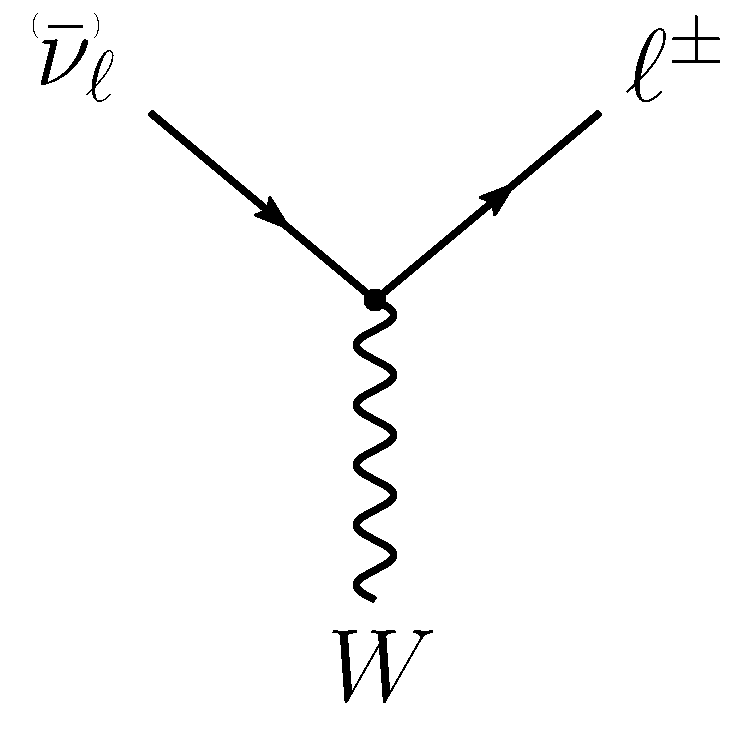
\includegraphics[width=0.49\linewidth]{figures/neutrinos_properties/feynman_CC_nu.pdf}
    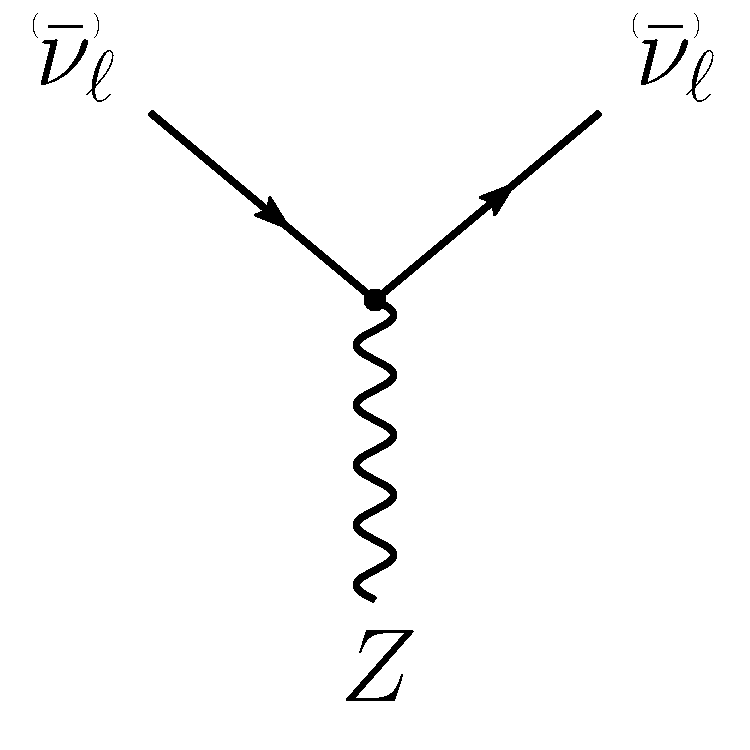
\includegraphics[width=0.49\linewidth]{figures/neutrinos_properties/feynman_NC_nu.pdf}
    \caption[Feynman diagrams of neutrino weak interactions]{Feynman diagrams of charged-current (left) and neutral-current (right) neutrino weak interactions, taken from \cite{ATerliuk}.}
    \labfig{weak_interactions}
\end{marginfigure}
\todo{Plot is missing + for W and 0 for Z boson.}

In the SM, weak interactions are mediated by the three massive bosons $\textbf{W}^+$, $\textbf{W}^-$, and $\textbf{Z}^0$ \sidecite{Thomson_Particle}.
The large boson masses ($m_{\textbf{W}}\sim\SI{80}{\gev}, m_{\textbf{Z}}\sim\SI{90}{\gev}$) result in a short range of the force of about \SI{10e-18}{\meter}.
Weak interactions carried by $\textbf{W}^\pm$ bosons are called CC interactions, because charge is transferred between the interacting particles.
In CC interactions, a neutrino is converted into its corresponding charged lepton or vice versa.
Neutral current (NC) interactions are those mediated by $\textbf{Z}^0$ bosons.
Here no charge is transferred.
The Feynman diagrams for CC and NC interactions are shown in \reffig{weak_interactions}.

The observed phenomenon of neutrino oscillations (see Section \refsec{neutrino_oscillations}) is based on the fact that there is a mass difference between the three neutrino mass eigenstates.


\section{Beyond the Standard Model}

\textbf{Open questions related to neutrinos:}
\begin{itemize}
    \item question of neutrino nature, e.g. dirac or majorana?
    \item absolute mass values? (mass ordering + absolute mass scale)
    \item is there leptonic cp violation and what is the precise delta\_cp value?
    \item what are the mixing angle values and is there a flavor principle
    \item is there additional effects like steriles, non-standard, lorentz violation
\end{itemize}


Are the fundamentals of the SM described above enough to explain \textit{all} observed phenomena? Gravity cannot be explained by the SM, as it is incompatible with general relativity. Neither can the SM explain some cosmological observations like dark matter, and the matter-antimatter asymmetry, and it does not predict neutrinos to have mass, which is experimentally proven by neutrino oscillations, so some extensions to the SM is needed in order to explain them.

Standard cosmology ($\Lambda$CDM\todo{Cite and/or sidenote this.}) assumes that equal amounts of matter and anti-matter were produced in the early universe. However, the universe today is dominantly made up of matter. This so-called \textit{baryon asymmetry} can be measured by the difference between the number densities of baryons and anti-baryons normalized to the number density of photons as
\begin{equation}
    \eta_B = \frac{n_B - n_{\bar{B}}}{n_\gamma}
    \;,
\end{equation}
where $n_B$, $n_{\bar{B}}$, and $n_\gamma$ are the number densities of baryons, anti-baryons, and photons, respectively. Baryons are the dominant component with  $\eta_B$ being observed to be around $6 \times 10^{-10}$\todo{cite this}. Leptogenesis and EW baryogenesis are scenarios that could explain this phenomenon, where the former could be realized by the existence of heavy RH neutrinos.

The observation of neutrino flavor conversions and neutrino oscillations in a multitude of experiments\sidecite{homestake, super_k_atm_osc, snolab_flavor_conv}\todo{cite neutrino oscillations/flavor conversions} is the strongest evidence for physics beyond the SM measured in laboratories. The observation that neutrinos change their flavor while they propagate through space can only be explained, if at least two neutrinos have a non-zero mass. From the measurements and cosmological observations, we know that the masses are very small as compared to the lepton masses. Neither their existence, nor their smallness is not predicted by the SM, but adding additional RH neutrinos states to the theory could explain the origin of the observed non-zero neutrino masses and could be tested for by searching for corresponding signatures in experiments. But the addition of RH neutrino fields is not the only possible explanation for neutrino masses. Radiative neutrino mass mechanisms could also explain their origin and their smallness, but those would need the introduction of additional symmetries to the theory.


Maybe also add this somehow: "From neutrino oscillation measurements the absolute mass scale cannot be determined, since they only depend on the mass differences, but there are upper limits on the sum of all neutrino masses from cosmological observations.
These upper limits are typically between $0.3$ and $1.3$\,eV \sidecite{PhysRevD.98.030001}."
"Actually \SI{0.8}{\electronvolt} \sidecite{katrin_nu_mass} from KATRIN and \SI{1.2}{\electronvolt} \sidecite{BOS_nu_masses, planck_nu_mass} from cosmological observations. 


\subsection{Mass Mechanisms}

\todo{namedrop RH=sterile=HNL and why they are called like this based on the SM EW Lagrangian introduced above}

There are no RH neutrinos in the SM and therefore the mass mechanism described in \refsec{fermion_masses}, which couples the Higgs field to LH and RH Weyl fields, predicts them to be massless. From experimental observations it is known that at least two of the three neutrino generations need to have a non-zero mass. Assuming the existence of RH neutrinos fields $\nu_{R}$, one way of producing the neutrino masses is by adding a Yukawa coupling term similar to the one for up-type quarks mentioned in \refsec{fermion_masses}, to write the full Yukawa Lagrangian as
\begin{equation}
    \mathcal{L}_\rm{Yukawa} = -Y^e_{ij} \bar{L}^i_L \Phi e^j_R - Y^\nu_{ij} \bar{L}^i_L \tilde{\Phi} \nu^j_R + h.c.
    \;,
    \labeq{dirac_yukawa_lagrangian}
\end{equation}
with $i,j$ running over the three generations of leptons $e$, $\mu$, and $\tau$, and $Y^e$ and $Y^\nu$ being the Yukawa coupling matrices. Diagonalizing the Yukawa coupling matrices through unitary transformations $U^e$ and $U^\nu$ leads to the \textbf{Dirac mass term} in the mass basis as
\begin{equation}
    \mathcal{L}^\rm{mass}_\rm{Dirac} = \frac{v}{\sqrt{2}} \left( \bar{e}_L M_e e_R - \bar{\nu}_L M_\nu \nu_R \right)
    \;,
    \labeq{dirac_mass_lagrangian}
\end{equation}
where $M_e$ and $M_\nu$ are the diagonal mass matrices of leptons and neutrinos, respectively. A purely Dirac mass term would not explain the smallness of the neutrino masses in a straightforward way. Only fine-tuning the Yukawa coupling constants to small values would lead to small neutrino masses.

An additional way of generating neutrino masses is by adding a Majorana mass term of the form
\begin{equation}
    \mathcal{L}_\rm{Majorana} = -\frac{1}{2} M_{ij} (\nu^i_R)^c \nu^j_R + h.c.
    \;,
    \labeq{majorana_mass_lagrangian}
\end{equation}
with $M_{ij}$ being the Majorana mass matrix and the indices $i, j$ running over all $N_R$ RH neutrino generations. The superscript $c$ denotes the charge conjugate field. Combining the charge conjugated RH neutrino fields with the LH neutrino fields as
\begin{equation}
    \boldsymbol{N} = \binom{\boldsymbol{\nu}_L}{\boldsymbol{\nu}_R^c}
    \;,
\end{equation}
with $\boldsymbol{\nu}_R$ containing the $N_R$ RH fields. The full neutrino mass Lagrangian is then given by the combined \textbf{Dirac and Majorana mass term} as
\begin{equation}
    \mathcal{L}^\rm{mass, \nu}_\rm{Dirac+Majorana} = \frac{1}{2} \boldsymbol{N}^T \hat{C} M^\rm{D+M} \boldsymbol{N} + h.c.
    \;,
    \labeq{dirac_and_Majorana_mass_lagrangian}
\end{equation}
and the mass matrix is given by
\begin{equation}
    M^\rm{D+M} = \begin{pmatrix}
    0 & (M^D)^T \\
    M^D & M^R
    \end{pmatrix}
    \;.
    \labeq{dirac_and_Majorana_mass_matrix}
\end{equation}
On top of explaining the origin of neutrino masses itself, a combined Dirac and Majorana mass term could also solve the question of their smallness. If the mass of the RH neutrinos is very large, the masses of the active neutrino flavors is suppressed, which is known as \textit{see-saw mechanism}.


\subsection{Neutrino Minimal Standard Model ($\nu$MSM)}



\subsection{Observational Avenues for Right-Handed Neutrinos}

\begin{itemize}
    \item oscillations searches for light steriles
    \item potential searches for heavy steriles
\end{itemize}


\subsection{Searching for Heavy Neutral Leptons} \labsec{HNL_mixing_constraints}


\subsubsection{Colliders}

\paragraph{Current Measurements}

LHC: proton-proton collider
sqrt(s): 7, 8, 13


ATLAS/CMS: nearly hermetic detectors around interaction, multiple searches for HNL scenarios
LHCB: forward detector, designed to search for new particles in decays of heavy hadrons

Type I Seesaw Results:

HNL production in GeV reange from : decays of heavy mesons, tau leptons, W bosons, H bosons, or top quarks
HNL decays: to lepton number conserving (dirac), or lepton number conserving and violating channels (majorana), depending on mass and mixing parameters, prompt and displaced decays are possible


Atlas results set constraints on mixing with e and mu:

Atlas in minimal extension: ~$10^-6$ with $U_mu4$ at 4-10 GeV
same for CMS: ~$10^-5$ with $U_mu4$ and $U_e4$ at 10-600 GeV

CMS: final state of 3 leptons (two opposite charged and nu) giving $U_mu4$ ~$4*10^-7$ at 8-14 GeV

the above mentioned (strong) constraints are mostly based on a model with one HNl coupling to one flavor
in type 1 seesaw at least 2 are needed to see the two SM nu masses, both coupling to several flavors
it was shown (cite) that re-interpreting these results with more than one HNL can lead to much weaker constraints and to compare results, the assumed model and couplings have to be considered
the strong reduction in constraints is due to the opening of new channels, to which the search may not be sensitive

more complex scenarios are possible and might produce various signatures, but are harder to measure: extended gauge symmetries, effective field theories

type III seesaw (HNL as SM EW triplets) can be observed as they are produced in pairs (no active-sterile mixing needed) and result in multi lepton states and high pt jets -> strong exclusion of masses below 790 GeV


LHCb: low mass and high mass results (above below mW), competitive in low mass

low mass channel: B+ -> mu+ N -> pi+ mu-, at order ~$10^-3$ for $U_mu4$ at 0.5-3.5 GeV

high mass channel: W+ -> mu+ mu+-jet, at order $10^-3$-$10^-2$ / $10^-4$-$10^-3$ for $U_mu4$ at 5-50 GeV for LNC/LNV


\paragraph{Future Colliders}

there is a shit ton of future colliders and/or experiments at the LHC planned, that have sensitivities to HNLs.. think about which/how to discuss them


\subsubsection{Nuclear Decay}

novel approach to search for HNLs through energy-momentum conservation measurements in nuclear reactions

mixing of HNL with electon nu/nubar would cause irregularities, interpretable as limits in \ue4 and m4


\paragraph{Beta Decay}

detect kinks in the energy spectra at $Q-m_4c^2$

m4 probable between energy detection threshold and Q value of the decay

tritium 3H: Q=18.6 keV

planned analysis in KATRIN and TRISTAN (1 to 18 keV mass) projected statistical upper limits (95) around $10^-7$ \ue4 (but will need detector upgrades)

in Project 8 measure the absolute neutrino mass using cyclotron radiation emission spectroscopy (CRES), may also be able to search for HNLs


atmospheric argon 39Ar: Q=565keV

DUNE: massive LArTPCs at long baseline (1300km) accelerator nu (1GeV), measure ionization charge of 39Ar beta decays: projected sensitivity in 20kev to 450keV mass range for \ue4 at $10^-7$ (requires substantial trigger development), without more like $10^-5$


\paragraph{Electron Capture}

requires total energy-momentum reconstruction of non nu final states in electron capture

e capture: pure 2-body decay of recoiling atom and electron neutrino (mono energetic)
measureing atom and associated de-excitation xray or auger electron, energy momentum conservation can be probed

separated non-zero missing mass peak would indicate HNL mixing with the electron neutrino/antineutrino

BeEST experiment: 100-850 keV mass, 7Be (Q=862keV), previous results at $10^-4$ \ue4, future sensitivity at $10^-7$ \ue4 after upgrades to the experiment

(proposed) HUNTER experiment: 20-300 keV mass (K-capture of 131Cs), "significantly improve current limits"


\paragraph{Reactor Searches}

MeV masses (up to 12) at short baseline reactor experiments (commercial or research reactors)

source of electron antineutrinos, therefore also HNL (if they mix)

visible channels: N to nu e+ e-, and N to nu gamma, nu gamma gamma, where the first dominates

pioneering analysis reports $10^-4$ \ue4 at 2-7 MeV mass range


many experiments exist at 5-25 meters from reactor core, at 100 MW research or 1 GW commercial reactors and 1-5 m3 volume detectors.. these are designed to adress reactor anomaly, but could most likely also proble decay in flight to electron positron


\subsubsection{Extracted Beamlines}


\subsubsection{Atmospheric and Solar}


\subsubsection{Cosmological and Astrophysical}



\begin{figure}
    \includegraphics{figures/hnl_simulation/decay_theory/hnl_decay_widths_up_to_1.0_GeV_log.png}
    \caption[HNL decay widths]{Decay widths of the HNL within the mass range considered, calculated based on the results from \cite{Coloma:2020lgy}. Given the existing constraints on $|U_{e4}|^{2}$ and $|U_{\mu4}|^{2}$, we consider that the corresponding decay modes are negligible.}
    \labfig{hnl_decay_modes_log_decay_width}
\end{figure}


\section{Atmospheric Neutrinos as Source of Heavy Neutral Leptons}

\todo{write some interlude to motivate atm. neutrinos as source for HNL searches/production etc.}


\subsection{Production of Neutrinos in the Atmosphere}

The analysis performed in this work is based on the sample of neutrinos observed in IceCube DeepCore at energies below \SI{100}{\gev}. At these energies, the flux exclusively originates in the Earth's atmosphere. Highly relativistic cosmic rays (protons and heavier nuclei \sidecite{PhysRevD.98.030001}) interact in the upper atmosphere, producing showers of secondary particles. Neutrinos are produced in decays of charged pions and kaons ($\pi$ and $K$ mesons) present in those showers, where the dominant contribution comes from the decay chain
\begin{equation}
    \begin{split}   
        \pi^\pm &\rightarrow \mu^\pm + \nu_\mu(\bar{\nu}_\mu)\;, \\
        \mu^\pm &\rightarrow e^\pm + \bar{\nu}_\mu(\nu_\mu) + \nu_e(\bar{\nu}_e)
        \;,
    \end{split}
    \labeq{pion_decay}
\end{equation}
where muon neutrinos $\nu_\mu$ and muons $\mu^\pm$ are produced in the first decay and both electron and muon neutrinos $\nu_{e/\mu}$ are produced in the second decay. Atmospheric muons, which are also produced in these decays, are the main background component for IceCube DeepCore analyses.

\begin{figure}
    \centering
    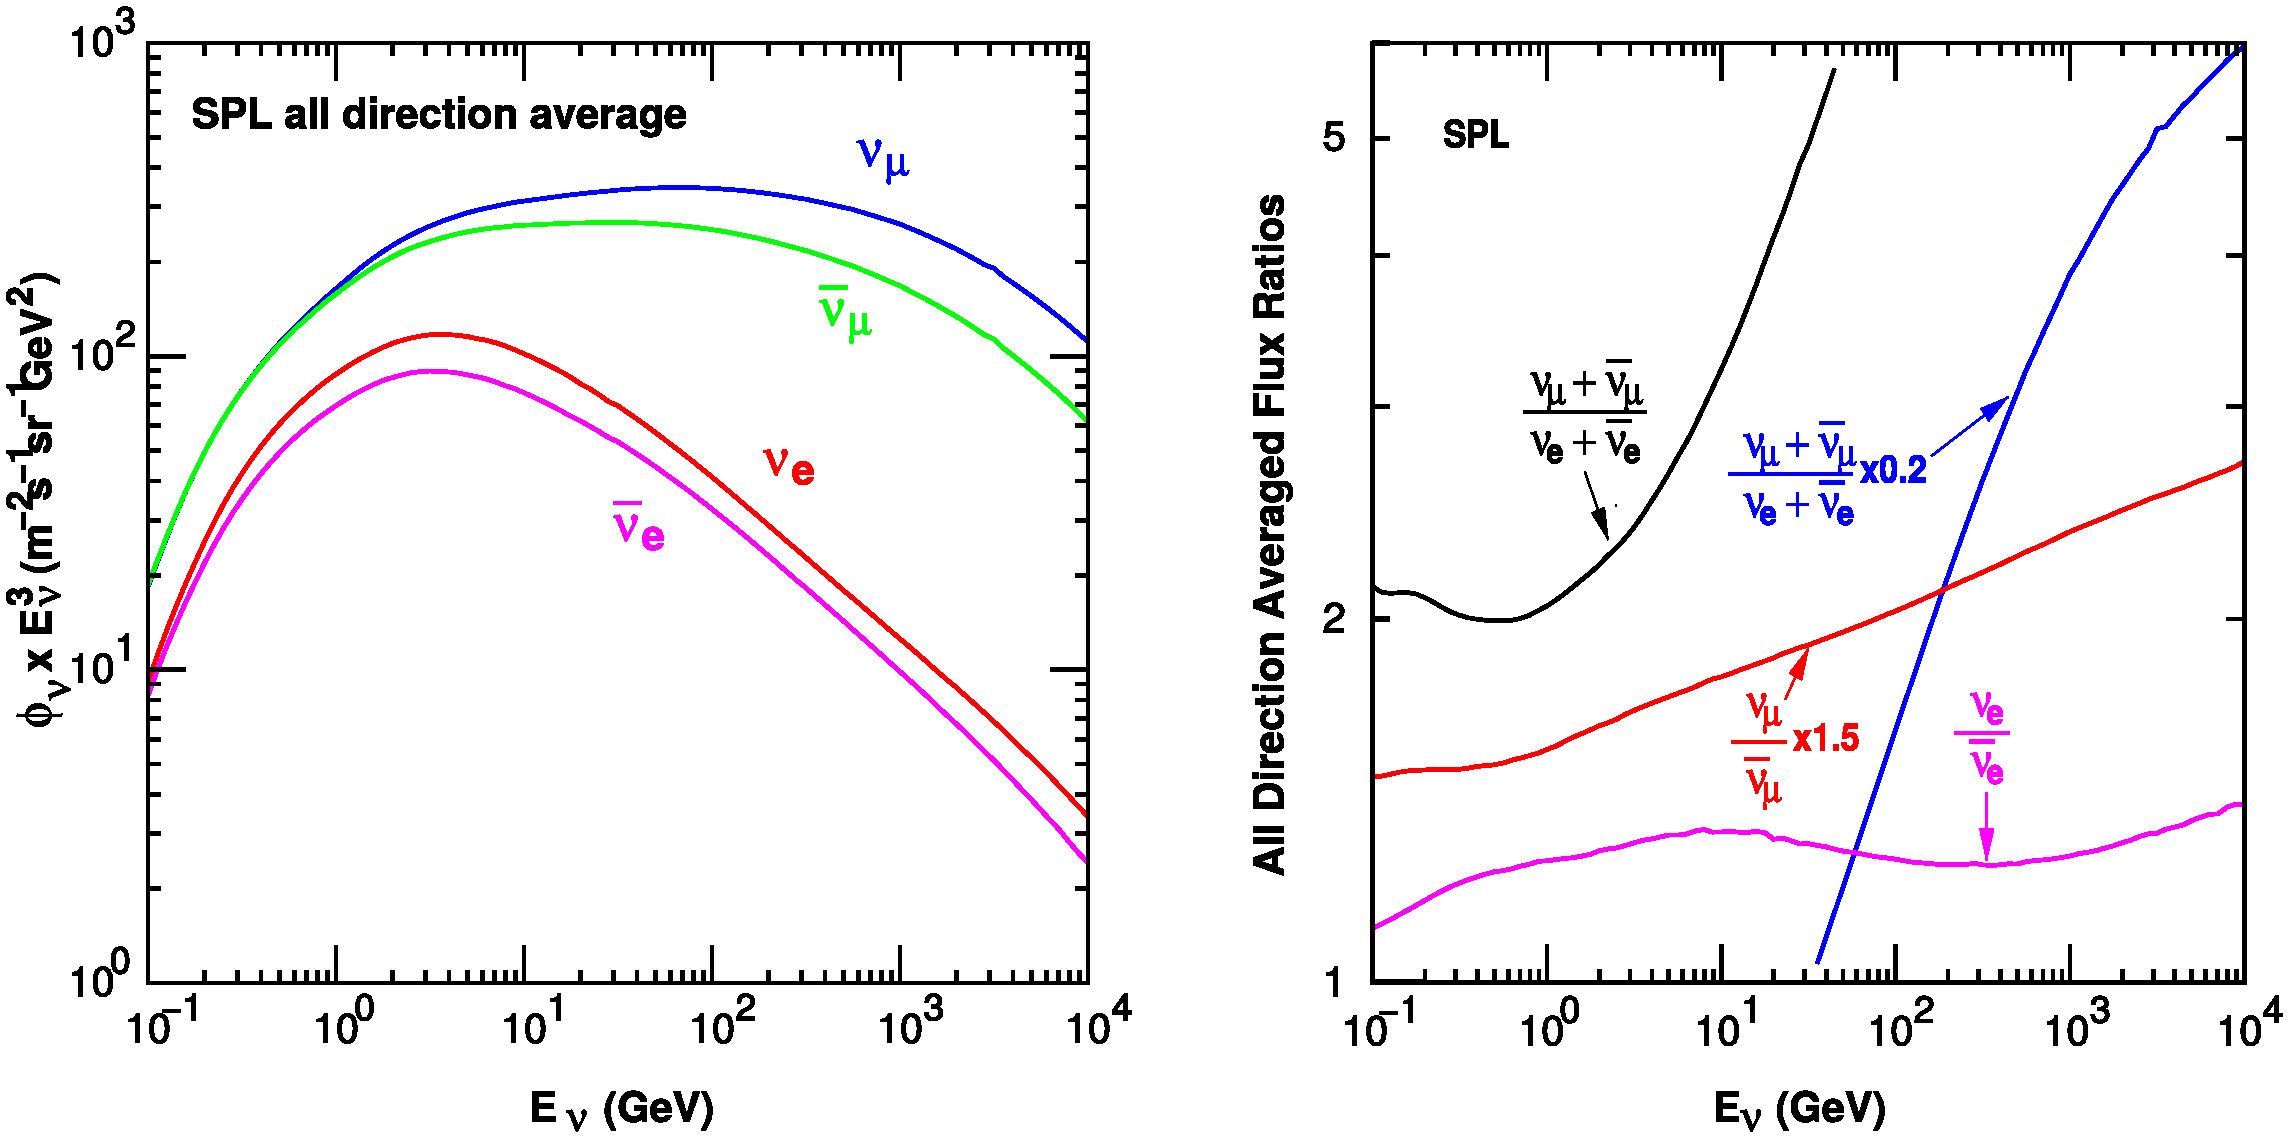
\includegraphics[width=1.0\textwidth]{figures/neutrinos_properties/Honda_alldir-spl_copy.pdf}
    \caption[Atmospheric neutrino fluxes]{The atmospheric fluxes of different neutrino flavors as a function of energy (left) and the ratios between muon neutrinos and electron neutrinos as well as the ratios between neutrinos and antineutrinos for both those flavors (right). Results from the calculations performed for the geographic South Pole, taken from \cite{PhysRevD.92.023004_Honda_Flux}.}
    \labfig{honda_flux}
\end{figure}

The different atmospheric flux components are shown in \reffig{honda_flux} (left), for a much broader energy range than relevant for this work. Both neutrinos and antineutrino fluxes are shown for electron  and muon neutrinos and all fluxes are the directionally averaged expectation calculated at the South Pole. Muon neutrinos are dominating the flux and from \refeq{pion_decay} the naive assumption would be that the ratio between muon and electron neutrinos is $(\nu_\mu+\bar{\nu}_\mu)/(\nu_e+\bar{\nu}_e)=2$. This is roughly true at energies below \SI{1}{\gev}, where all muons decay in flight, but at larger energies muons can reach the detector before decaying, which increases the ratio to approximately 10:1 at around \SI{100}{\gev}. Additionally, kaon decays start to contribute which also increases the number of muons and muon neutrinos. The increasing ratio can be seen in \reffig{honda_flux} (right), which also shows the ration between neutrinos and antineutrinos for both flavors.

Charged mesons or tau particles can also be produced in cosmic ray interactions. Their decays lead to the production of tau neutrinos. At the energies relevant for this work however, the resulting tau neutrino flux is negligible as compared to the muon neutrino flux \sidecite{2015EPJWC..9908001F_lepton_fluxes} and is not considered in the analysis. This is because both charged mesons and tau particles are much heavier than pions and kaons and therefore their production is suppressed at high energies.\todo{Say something about atmospheric neutrino flux uncertainties, based on recent JP/Anatoli papers.}
% It should be stated here that there is a rather large uncertainty on the normalization of the atmospheric neutrino flux on the order of 20-30\,\% \sidecite{PhysRevD.75.043006_neutino_flux_honda} in the energy region of interest.
% This is mainly due to uncertainties in the primary cosmic ray spectrum and modeling of the hadronic interactions.\todo{SB:
% I don't think this is true - the normalization is known to ~5\% if you trust Anatoli/Juan Pablo. Please have a look at more recent publications on this topic.}


\subsection{Interactions with Nuclei}

The neutrino detection principle of IceCube DeepCore is explained in \refch{icecube} and relies on the weak interaction processes between neutrinos and the nuclei of the Antarctic glacial ice. At neutrino energies above \SI{5}{\gev}, the cross-sections are dominated by \textbf{\textit{deep inelastic scattering (DIS)}}, where the neutrino is energetic enough to resolve the underlying structure of the nucleons and interact with one of the composing quarks individually. As a result the nucleon breaks and a shower of hadronic secondary particles is produced. Depending on the type of interaction, the neutrino either remains in the final state for NC interactions or is converted into its charged lepton counterpart for CC interactions. The CC DIS interactions have the form
\begin{equation}
    \begin{split}
        \nu_l + N \rightarrow l^- + X \;, \\
        \bar{\nu}_l + N \rightarrow l^+ + X \;, \\
    \end{split}
    \labeq{dis_cc}
\end{equation}
where $\nu_l$/$\bar{\nu}_l$ and $l^-$/$l^+$ are the neutrino/antineutrino and its corresponding lepton/antilepton, and $l$ can be either an electron, muon, or tau. $N$ is the nucleon and $X$ stands for any set of final state hadrons. The NC DIS interactions are
\begin{equation}
    \begin{split}
    \nu_l + N & \rightarrow \nu_l + X \; \rm{and} \\
    \bar{\nu_l} + N & \rightarrow \bar{\nu_l} + X \;.
    \end{split}
    \labeq{dis_nc}
\end{equation}
\reffig{dis_feynman} shows the Feynman diagrams for both processes
\begin{figure}[h]
    \centering
    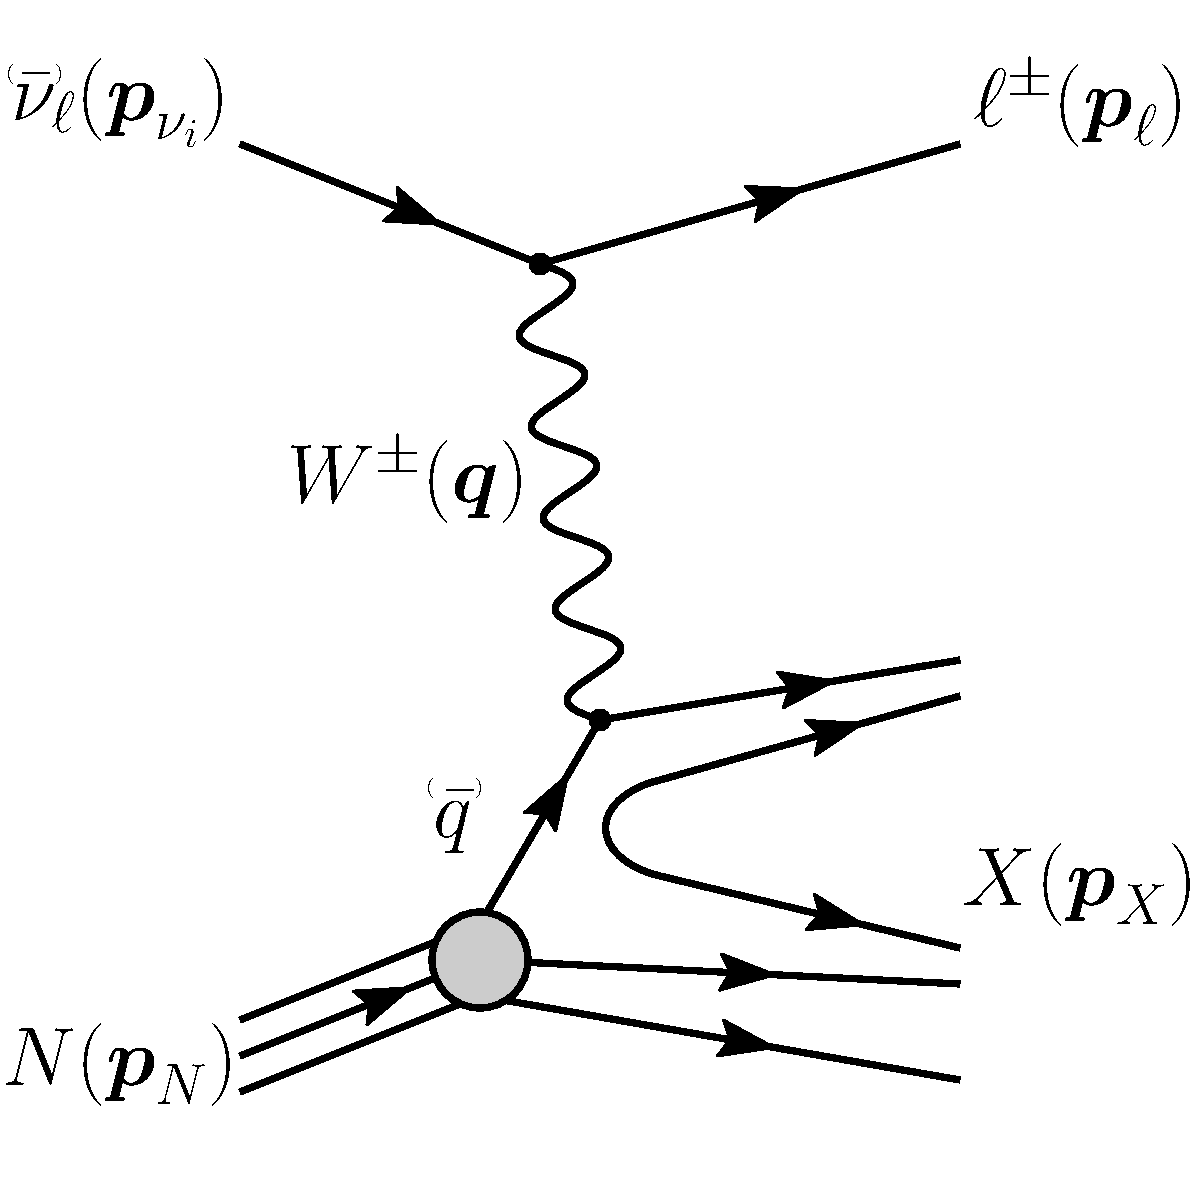
\includegraphics[width=0.4\linewidth]{figures/neutrinos_properties/feynman_DIS_CC_nu_new.pdf}
    \hspace{0.8cm}
    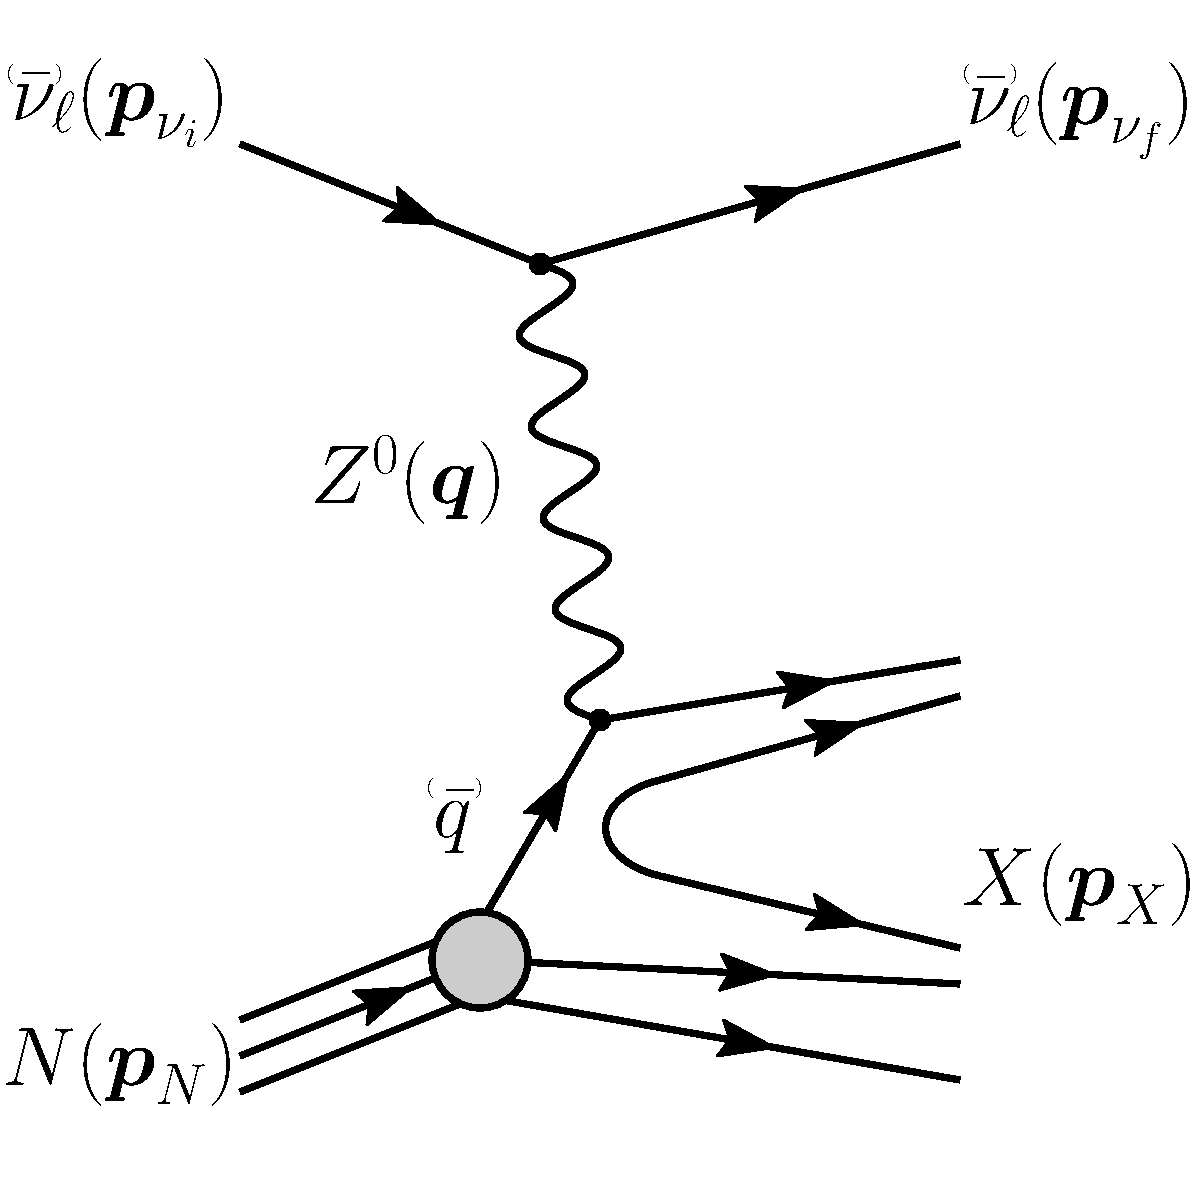
\includegraphics[width=0.4\linewidth]{figures/neutrinos_properties/feynman_DIS_NC_nu_new.pdf}
    \caption[Neutrino-nucleon deep inelastic scattering]{Feynman diagrams for deep inelastic scattering of a neutrino with a nucleon via charged-current (left) and neutral current (right) interactions. $\boldsymbol{p}_{\nu_i}$, $\boldsymbol{p}_{N}$ and $\boldsymbol{p}_{\nu_f}$, $\boldsymbol{p}_{l}$, $\boldsymbol{p}_{N}$ are the input and output four-momenta, while $\boldsymbol{q}$ is the momentum transfer. Taken from \cite{ATerliuk}.}
    \labfig{dis_feynman}
\end{figure}
DIS interactions have a roughly linear energy dependent cross-section above $\sim$\SI{20}{\gev} and are well measured and easy to theoretically calculate. They are the primary interaction channel for neutrinos detected with IceCube.

At energies below \SI{5}{\gev}, \textbf{\textit{quasi-elastic scattering (QE)}} and \textbf{\textit{resonant scattering (RES)}} become important. At these energies the neutrinos interact with the approximately point-like nucleons, without breaking them up in the process. RES describes the process of a neutrino scattering off a nucleon producing an excited state of the nucleon in addition to a charged lepton. It is the dominant process at \SIrange{1.5}{5}{\gev} for neutrinos and \SIrange{1.5}{8}{\gev} for antineutrinos. Below \SI{1.5}{\gev} QE is the main process, where protons are converted to neutrons in antineutrino interactions and vice-versa for neutrino interactions. Additionally, a charged lepton corresponding to the neutrino/antineutrino flavor is produced. The cross-sections of QE and RES scattering processes are not linear in energy and the transition region from QE/RES to DIS is poorly understood. The total cross-sections and their composition is shown in \reffig{neutrino_cross_sections}. It can be seen that the interaction cross-sections are very small at the order of $10^{-38}\mathrm{\,cm}^2$. This is the reason why very large volume detectors are required to measure atmospheric neutrinos with sufficient statistics to perform precision measurements of their properties. The interaction length of a neutrino with $E_\nu = \SI{10}{\gev}$ is of $\mathcal{O}(\SI{10e10}{\kilo\meter})$, for example.

\begin{figure*}[h]
	\centering
    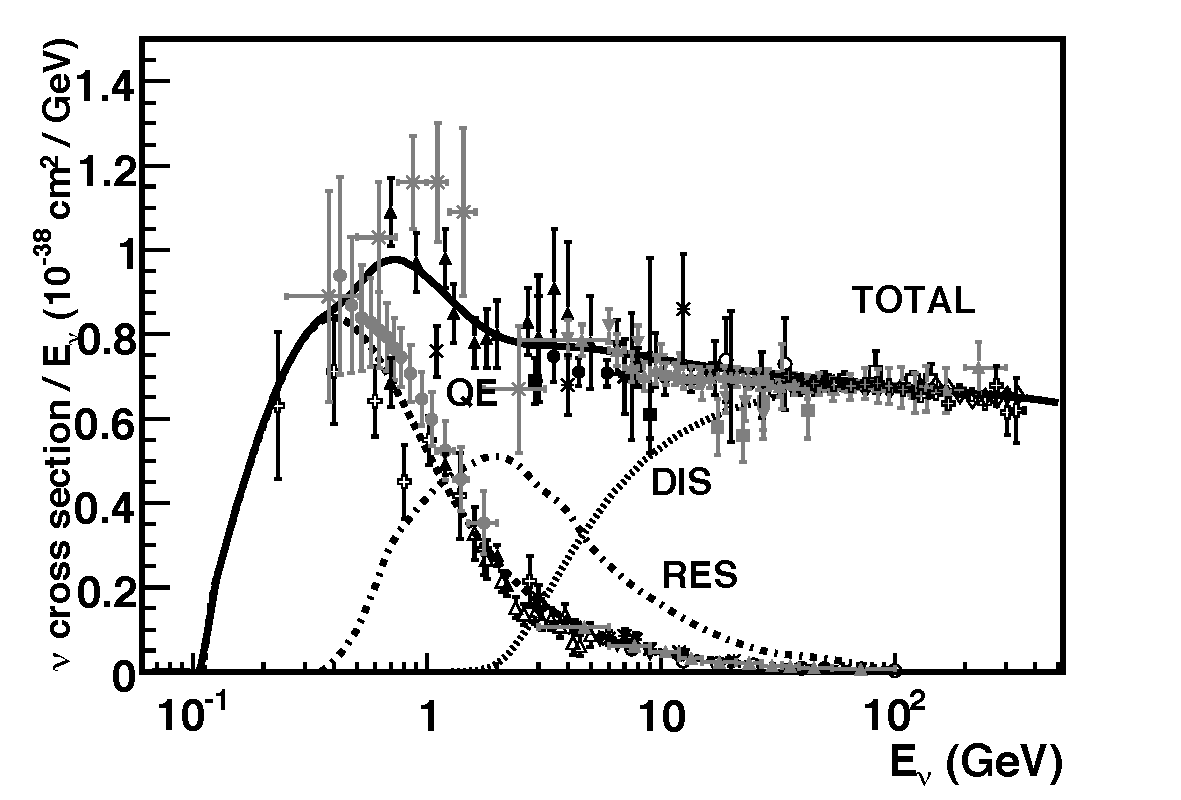
\includegraphics[width=0.495\linewidth]{figures/neutrinos_properties/cc_inclusive_nu.pdf}
    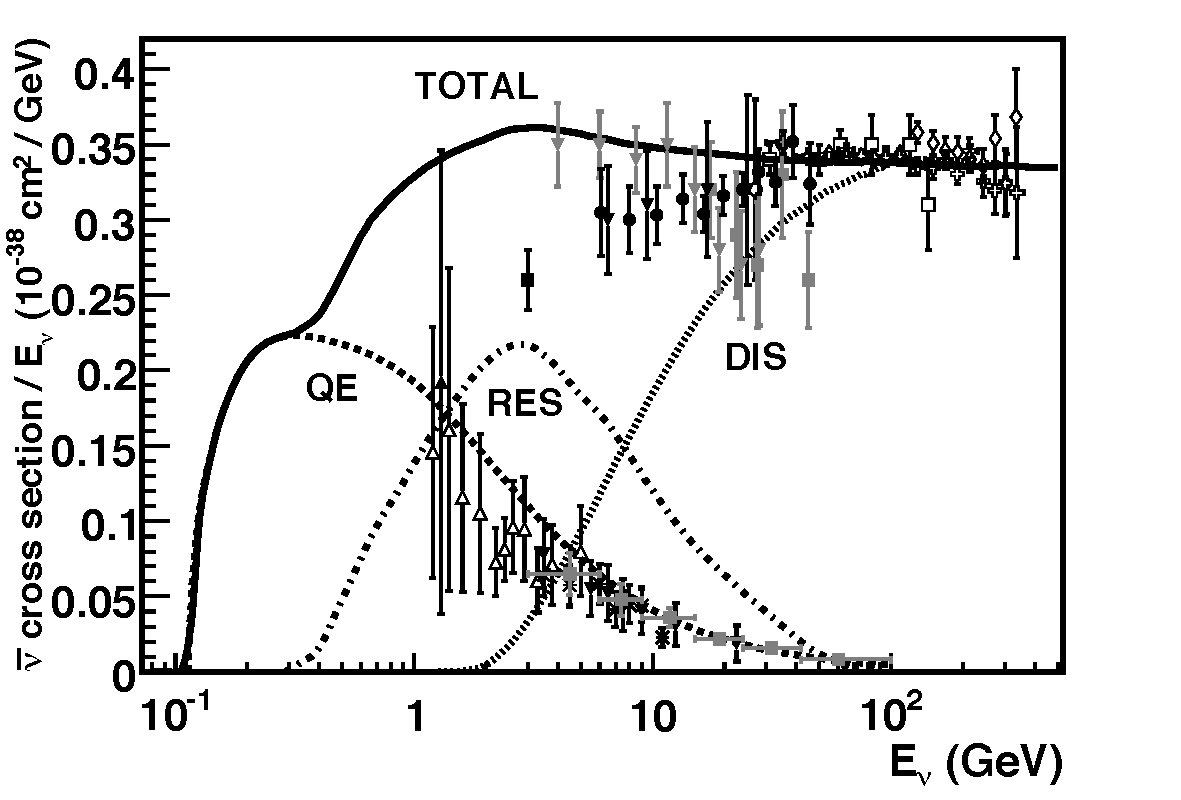
\includegraphics[width=0.495\linewidth]{figures/neutrinos_properties/cc_inclusive_nubar.pdf}
	\caption[Total inclusive neutrino-nucleon cross-sections]{Total neutrino (left) and antineutrino (right) per nucleon cross-section divided by neutrino energy plotted against energy.
    The three main scattering processes quasi-elastic scattering (QE), resonant scattering (RES), and deep-inelastic scattering (DIS) are shown. Taken from \cite{Formaggio_Cross_Sections}.}
    \labfig{neutrino_cross_sections}
\end{figure*}


\subsection{Oscillations} \labsec{neutrino_oscillations}

So far we have described neutrinos in their flavor eigenstates, which are relevant for weak interactions. In the SM three-neutrino model the weak flavor states are $\nu_e, \nu_\mu$, and $\nu_\tau$, which relate them to the charged leptons they interact with in CC interactions. There is a second way of describing neutrino wave functions based on their Hamiltonian eigenvalues \sidecite{BILENKY1978225}, namely as the mass eigenstates $\nu_1, \nu_2$, and $\nu_3$. These states are related to the flavor eigenstates by the unitary, 3x3 \textit{Pontecorvo-Maki-Nakagawa-Sakata (PMNS)} matrix $U$, where the flavor states are a superposition of the mass states as
\begin{equation}
    \ket{\nu_\alpha} = \sum_kU^*_{\alpha k}\ket{\nu_k}
    \;,
    \labeq{neutrino_mixing}
\end{equation}
with the weak flavor states $\ket{\nu_\alpha}$, $\alpha=e,\mu,\tau$, and the mass states $\ket{\nu_k}$ with $k=1,2,3$. The mixing matrix can be parameterized as \sidecite{PhysRevD.98.030001}
\begin{equation}
    U=\left( 
    \begin{matrix}
        1 & 0 & 0 \\
        0 & c_{23}  & s_{23} \\
        0 & -s_{23} & c_{23} 
    \end{matrix}
    \right) 
    \left( 
    \begin{matrix}
        c_{13} & 0 & s_{13}e^{-i\delta_{CP}} \\
        0 & 1 & 0\\
        -s_{13} e^{i\delta_{CP}} & 0 & c_{13}
    \end{matrix}
    \right) 
    \left( 
    \begin{matrix}
        c_{12} & s_{12} & 0 \\
        -s_{12} & c_{12} & 0\\
        0 & 0 & 1
    \end{matrix} 
    \right)  
    \;,
    \labeq{PMNS_matrix}
\end{equation}
where $c_{ij}=\cos\theta_{ij}$ and $s_{ij}=\sin\theta_{ij}$ are cosine and sine of the mixing angle $\theta_{ij}$, that defines the strength of the mixing between the mass eigenstates $i$ and $j$, and $\delta_{CP}$ is the neutrino CP-violating phase.\todo{add current BF values from nufit or so?}

Describing neutrinos in their mass state is crucial to understand their propagation through space and time. Their propagation in vacuum can be expressed by applying a plane wave approach, where the mass eigenstates evolve as
\begin{equation}
    \ket{\nu_k(t)} = e^{-iE_kt/\hbar}\ket{\nu_k}
    \;.
    \labeq{flavor_time_evol}
\end{equation}
The energy of the mass eigenstate $\ket{\nu_k}$ is $E_k=\sqrt{\vec{p}^2c^2+m_k^2c^4}$, with momentum $\vec{p}$ and mass $m_k$, $\hbar$ is the reduced Planck constant, and c is the speed of light in vacuum. The existence of non-zero, non-equal masses and the neutrino mixing relation in \refeq{neutrino_mixing}, lead to the observed phenomenon of neutrino oscillations. Oscillations mean that a neutrino changes from its initial flavor, that it was produced with, to another flavor and back after traveling a certain distance. A neutrino is produced as a flavor eigenstate $\ket{\nu_\alpha}$ in a CC weak interaction, but its propagation happens as the individual mass states it is composed of. The probability of finding the neutrino with initial flavor $\ket{\nu_\alpha}$ in the flavor state $\ket{\nu_\beta}$ after the time $t$ is calculated as
\begin{equation}
    P_{\nu_\alpha \rightarrow \nu_\beta}(t)
    =
    |\braket{\nu_\beta|\nu_\alpha(t)}|^2
    \;,
    \labeq{fermis_golden_rule}
\end{equation}
by applying Fermi's Golden Rule \sidecite{1927RSPSA.114..243D}, which defines the transition rate from one eigenstate to another by the strength of the coupling between them. This coupling strength is the square of the matrix element and using the fact that the mixing matrix is unitary ($U^{-1}=U^\dagger$) to describe the mass eigenstates as flavor eigenstates, we find the time evolution of the flavor state $\ket{\nu_\alpha(t)}$, which can be inserted into \refeq{fermis_golden_rule} to find the probability as
\begin{equation}
    P_{\nu_\alpha \rightarrow \nu_\beta}(t)
    =
    \sum_{j,k}U^*_{\beta j}U_{\alpha j}U_{\beta k}U^*_{\alpha k}e^{-i(E_k-E_j)t/\hbar}
    \;.
    \labeq{probability_raw}
\end{equation}
The indices $j$ and $k$ run over the mass eigenstates. We can approximate the energy as
\begin{equation}
    E_k \approx E+\frac{c^4m^2_k}{2E} \hspace{0.25cm} \longrightarrow \hspace{0.25cm} E_k-E_j \approx \frac{c^4\Delta m^2_{kj}}{2E}
    \;,
\end{equation}
for small neutrino masses compared to their kinetic energy. Here, $\Delta m^2_{kj}=m^2_k-m^2_j$ is the mass-squared splitting between states $k$ and $j$. Replacing the time in \refeq{probability_raw} by the distance traveled by relativistic neutrinos $t\approx L/c$ we get
\begin{equation}
    \begin{split}
        P_{\nu_\alpha \rightarrow \nu_\beta}(t)
        = 
        \delta_{\alpha \beta}
        -
        4\sum_{j>k}&\textbf{Re}(U^*_{\beta j}U_{\alpha j}U_{\beta k}U^*_{\alpha k})\textrm{sin}^2\Big( \frac{c^3\Delta m^2_{kj}}{4E\hbar}L \Big) \\
        +
        2\sum_{j>k}&\textbf{Im}(U^*_{\beta j}U_{\alpha j}U_{\beta k}U^*_{\alpha k})\textrm{sin}^2\Big( \frac{c^3\Delta m^2_{kj}}{4E\hbar}L \Big)
        \;,
    \end{split}
    \labeq{probability_detailed}
\end{equation}
which is called the survival probability if $\alpha=\beta$, and the transition probability if $\alpha\neq\beta$. Once again, this probability is only non-zero if there are neutrino mass eigenstates with masses greater than zero. Additionally, there must be a mass-squared difference $\Delta m^2$ and non-zero mixing between the states. Since we assumed propagation in vacuum in \refeq{flavor_time_evol}, the transition and survival probabilities correspond to vacuum mixing. \todo{say something about how this changes with matter}


\subsection{Testing Heavy Neutral Leptons with Atmospheric Neutrinos} \labsec{double_cascade_morphology}


\subsubsection{The Minimal Standard Model Extension} \labsec{HNL_model_to_be_tested}

\todo{Re-write/re-formulate this section (copied from HNL technote).}

Extensions to the Standard Model (SM) that add \textit{Heavy Neutral Leptons (HNLs)} provide a good explanation for the origin of neutrino masses through different seesaw mechanisms \sidecite{PTP.64.1103}.
\begin{figure}
  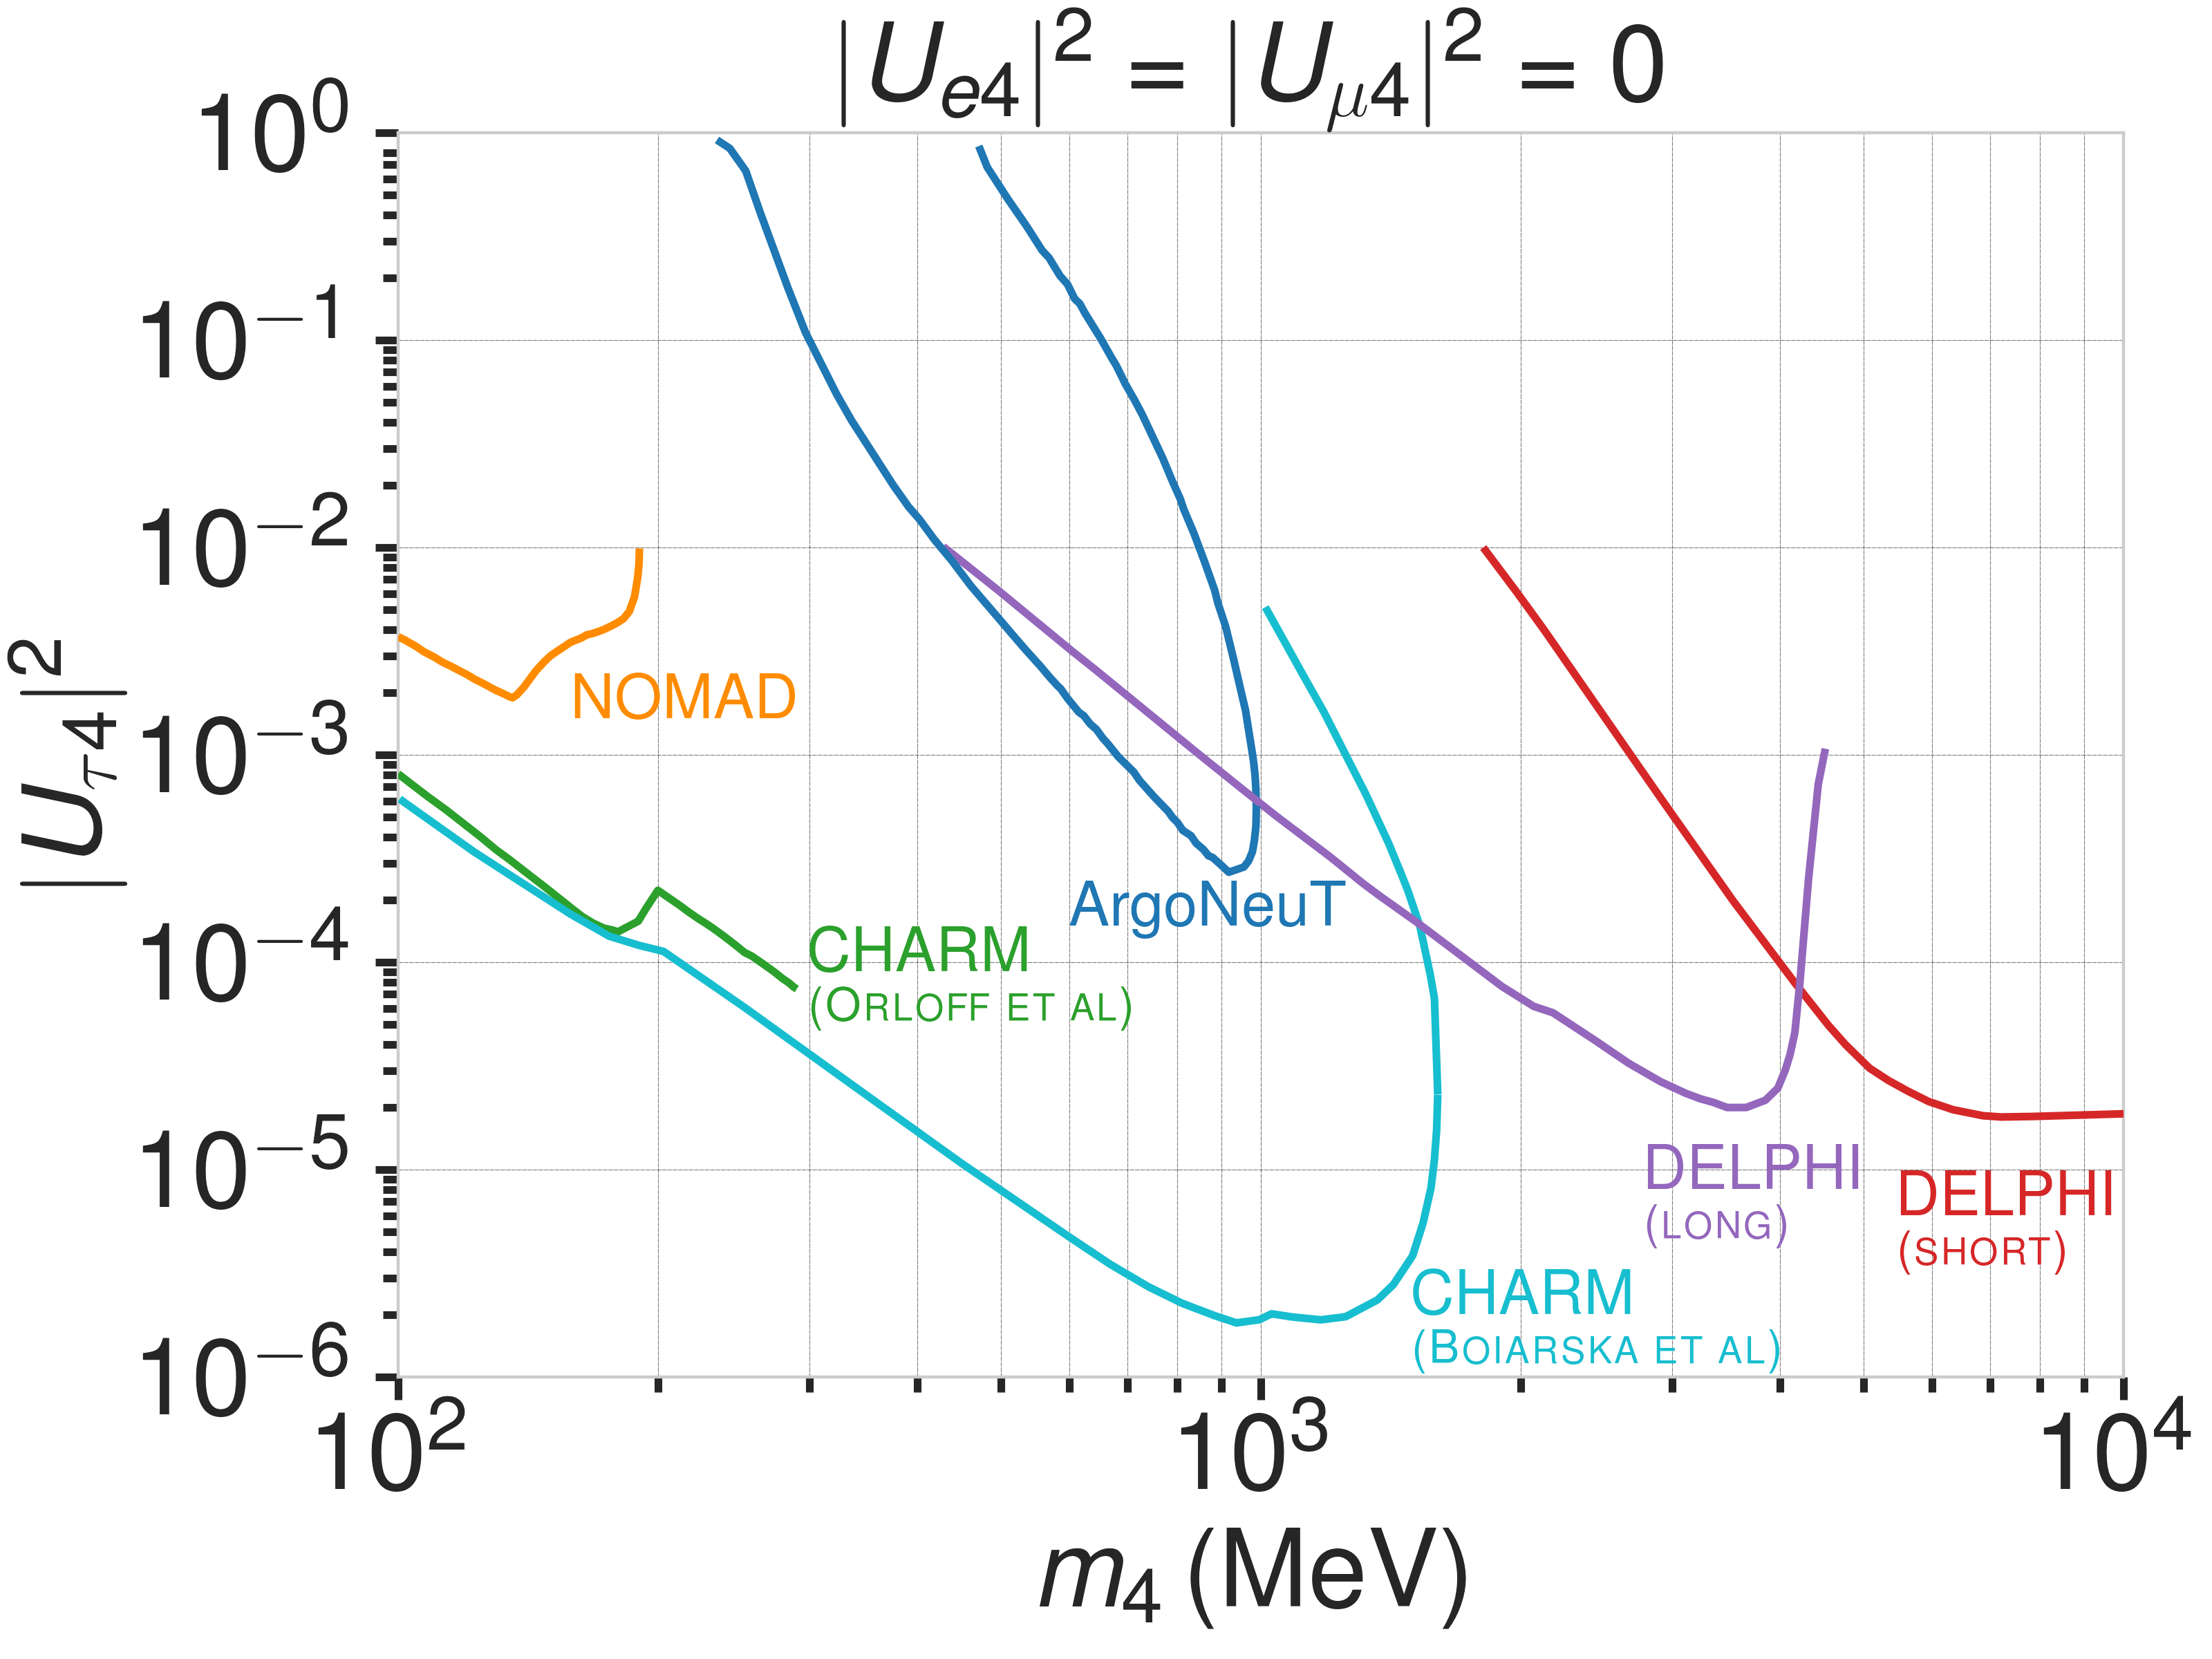
\includegraphics{figures/hnl_simulation/theory/UtauN_custom_plots_LF_grid_white.png}
  \caption[Current $|U_{\tau4}^2|-m_4$ limits]{Current $|U_{\tau4}^2|-m_4$ limits from NOMAD \cite{NOMAD:2001eyx}, ArgoNeut \cite{ArgoNeuT:2021clc}, CHARM \cite{Orloff:2002de, Boiarska:2021yho}, and DELPHI \cite{DELPHI:1996qcc}.}
  \labfig{boundsUtau}
\end{figure}
While the mixing with $\nu_{e/\mu}$ is strongly constrained\todo{Produce similar styled plot for these limits} ($|U_{\alpha4}^2| \lesssim 10^{-5}-10^{-8}, \alpha=e,\mu$), the mixing with $\nu_{\tau}$ is much harder to probe due to the difficulty of producing and detecting $\nu_\tau$. \reffig{boundsUtau} shows the current limits on the $\tau$-sterile mixing space for HNL masses between $0.1$\,GeV-$10$\,GeV. As was first pointed out in \sidecite{Coloma:2017ppo}, the atmospheric neutrino flux observed in IceCube offers a way to constrain the neutrino-HNL mixing parameters. By using the large fraction of atmospheric $\nu_{\mu}$ events that oscillate into $\nu_{\tau}$ before they reach the detector, the less constrained $\tau$-sterile mixing space can be explored. In this document, we present the methodology and strategy of a search for HNLs with IceCube DeepCore. These additional RH neutrinos can be included in the Standard Model (SM) by extending the PMNS matrix to at least a 3x4 matrix as
\begin{equation}
    \begin{pmatrix}
    \nu_{e}\\
    \nu_{\mu}\\
    \nu_{\tau}\\
    \nu_{s}\\
    \end{pmatrix}
    =
    \begin{pmatrix}
    U_{e1} & U_{e2} & U_{e3} & U_{e4}\\
    U_{\mu1} & U_{\mu2} & U_{\mu3} & U_{\mu4}\\
    U_{\tau1} & U_{\tau2} & U_{\tau3} & U_{\tau4}\\
    U_{s1} & U_{s2} & U_{s3} & U_{s4}\\
    \end{pmatrix}
    \begin{pmatrix}
    \nu_{1}\\
    \nu_{2}\\
    \nu_{3}\\
    \nu_{4}\\
    \end{pmatrix}
    \;,
    \labeq{4_by_4_mixing_matrix}
\end{equation}
where the components with index $4$ define the mixing between the flavor states and the fourth sterile mass state, respectively. Note here that this is not a theoretically fully consistent picture, but rather the phenomenologically minimal model to be tested by this analysis. This can hopefully be put into the larger context of several fully consistent models, later. Due to the singlet nature of the RH neutrinos, they only interact weakly, inheriting these interactions from their LH neutrino counterparts via mixing. This mixing of the HNLs with the electron, muon, and tau neutrinos can be probed and constrained as a function of the HNL mass by searching for their production and decay. In \sidecite{Coloma:2017ppo, Coloma:2019qqj} this search is mainly motivated through two experimental arguments\todo{This section really needs to be re-written to motivate the search for HNLs from a more generic point of view (e.g. to explain neutrino masses)}.
% First, a decaying sterile neutrino could explain the low-energy excess (LEE) that is observed in the MiniBooNE data \sidecite{PhysRevLett.110.161801}.
Secondly, IceCube is ideally placed to explore the yet unconstrained $|U_{\tau4}|^{2}-m_{4}$ phase-space that is not easily accessible by accelerator-based experiments.


In order to probe the $\tau$-sterile mixing parameter, it is required to look at interactions involving $\tau$ neutrinos. However, most neutrinos produced in cosmic ray interactions with the atmosphere are $\nu_{e}$ or $\nu_{\mu}$. Therefore, we need these neutrinos to oscillate to the $\tau$ flavor before reaching the detector. For this to happen at the considered energies a traveled distance of the order of the earth diameter is necessary. This is why our signal is mostly up-going and passing through the whole earth.\todo{This section definitley needs to be elaborated in a little more detail}

To explain the signature we can observe in IceCube we first have to revisit the weak interactions that the HNL inherits from its LH counterpart through mixing. We will be following the derivation in \sidecite{Coloma:2020lgy}. Extending the SM by n additional RH neutrinos, $\nu_i$ ($i=3+n$), leads to the mass Lagrangian
\begin{equation}
    \mathcal{L}_{\nu }^{\rm mass} \supset - \sum _{\alpha = e,\mu ,\tau} \sum _{i=4}^{3+n} Y_{\nu , \alpha i} {\overline{L}}_{L,\alpha} {\tilde{\phi }} \nu_{i} - \frac{1}{2} \sum _{i=4}^{3+n} M_{i} {\overline{\nu}}_{i} \nu^c_{i} + h.c.,
    \label{eq:hnl_mass_lagrangian}
\end{equation}
in a basis where the Majorana mass terms are diagonal. $Y_{\nu , \alpha i}$ are the Yukawa couplings to the lepton doublets and $M$ the Majorana masses for the heavy singlets. $L_{L,\alpha}$ stands for the SM LH lepton doublet of flavor $\alpha$ while $\phi$ is the Higgs field, and ${\tilde{\phi }} = i \sigma _2 \phi ^*$ and $\nu^c_{i} \equiv C {\bar{\nu}}_{i}^t$, with $C = i \gamma _0 \gamma _2$ in the Weyl representation. The full neutrino mass matrix with the Higgs vacuum expectation value $v/\sqrt{2}$ reads\todo{Not adding information about the case where the neutrinos have Dirac or pseudo-Dirac masses}
\begin{equation}
    {\mathcal {M}} = \left( \begin{array}{cc} {\mathbf {0}}_{3\times 3} &{} Y_\nu v/\sqrt{2} \\ Y_\nu ^t v/\sqrt{2} &{} M \end{array} \right),
    \label{eq:majorana_mass_matrix}
\end{equation}
and can be diagonalized by a $(3+n)$ x $(3+n)$ full unitary roation $U$, that itself leads to neutrino masses upon diagonalization, additionally manifesting the mixing between active neutrinos and heavy states. The resulting model consists of 3 light SM neutrino mass eigenstates $\nu_i$ ($i=1,2,3$) and n heavier states, as introduced above. The flavor states will now consist of a combination of light and heavy states
\begin{equation}
    \nu _\alpha = \sum _{i=1}^{3+n} U_{\alpha i} \nu_i,
    \label{equ:extend_neutrin_flavor_mass_relation}
\end{equation}
and the leptonic part of the EW Lagrangian can be written as
\begin{equation}
    \begin{aligned}
        \mathcal{L}^{\ell}_{\rm EW} &= \frac{g}{\sqrt{2}}W^+_\mu \sum _{\alpha } \sum _{i} U_{\alpha i}^* {\bar{\nu}}_{i}\gamma ^\mu P_L \ell _\alpha + \frac{g}{4c_w} Z_\mu \nonumber \\& \times \left\{ \sum _{i, j} C_{ij} {\bar{\nu}}_{i}\gamma ^\mu P_L \nu_j + \sum _\alpha {\bar{\ell }}_\alpha \gamma ^\mu \left[ 2s_w^2P_R\!-\!(1\!-\!2s_w^2)P_L \right] \ell _\alpha \right\} \nonumber + h.c.,
    \end{aligned}
    \label{eq:leptonic_ew_lagrangian}
\end{equation}
where $c_w \equiv \cos \theta _w$, $s_w \equiv \sin \theta _w$, and $\theta _w$ the SM weak mixing angle or \textit{Weinberg angle}. $P_L$ and $P_R$ are the left and right projectors, respectively, while
\begin{equation}
    C_{ij} \equiv \sum _\alpha U^*_{\alpha i} U_{\alpha j}.
    \label{eq:general_squared_mixing}
\end{equation}
The indices now sum over all $(3+n)$ flavor and mass states.

Based on this formulation and assuming that only the mixing with the tau sector is open ($|U_{\alpha4}^2|=0, \alpha=e,\mu$), the relevant production diagram of the HNL can be drawn as shown in \reffig{HNL_production}. Alongside the fourth heavy mass state, a Hadronic cascade is produced. The heavy mass state will travel for some distance (dependent on mass and mixing) before it decays. The subsequent decay processes are depicted in \reffig{HNL_decay}. It can be a CC or NC decay and both leptonic and mesonic modes are possible (dependent on the mass). This will produce a tau or a tau neutrino and another cascade that can be EM or Hadronic. The branching ratios corresponding to the decay modes of the HNL for the mass range of interest (i.e. between \SI{100}{\mev} and 1\,GeV) are shown in \reffig{hnl_decay_modes_log_branching_ratio} as a function of the HNL mass.
\begin{figure}[!htb]
    % \footnotesize
    \centering
    \begin{fmffile}{figures/feynman_diagrams/diag_HNL_production}
        \begin{fmfgraph*}(210,70)
        \fmfleft{i1,i2}
        \fmfright{o1,o2}
        \fmf{fermion,label=$q$,label.side=right}{i1,v1,o1}
        \fmf{fermion,label=$\nu_{\tau}$,label.side=left}{i2,v2}
        \fmf{fermion,label=$\nu_{4}$,label.side=left}{v2,o2}
        \fmf{photon,label=$Z$}{v1,v2}
        \fmflabel{$|U_{\tau 4}|^2$}{v2}
        \end{fmfgraph*}
    \end{fmffile}
    \caption[Feynman diagram of HNL up-scattering process]{Production of a sterile neutrino in the up-scattering of a tau neutrino.}
    \labfig{HNL_production}
\end{figure}

\begin{figure}[!htb]
    % \footnotesize
    \centering
    \begin{fmffile}{figures/feynman_diagrams/diag_HNL_decay_NC}
        \begin{fmfgraph*}(175,70)
        %\fmfstraight
        \fmfleft{i}
        \fmfright{o1,o2,o3}
        \fmf{fermion,tension=3.,label=$\nu_{4}$,label.side=left}{i,v1}
        \fmfv{label=$|U_{\tau 4}|^2$,label.angle=90}{v1}
        \fmf{fermion,label=$\nu_{\tau}$,label.side=left}{v1,o3}
        \fmf{photon,tension=3,label=$Z$,label.side=right}{v1,v2}
        \fmf{fermion,tension=3,label=$f/q/q$,label.side=left}{v2,o2}
        \fmf{fermion,tension=3,label=$\bar{f}/\bar{q}/\bar{q'}$,label.side=left}{o1,v2}
        \end{fmfgraph*}
        \end{fmffile}
        \begin{fmffile}{figures/feynman_diagrams/diag_HNL_decay_CC}
        \begin{fmfgraph*}(175,70)
        %\fmfstraight
        \fmfleft{i}
        \fmfright{o1,o2,o3}
        \fmf{fermion,tension=3.,label=$\nu_{4}$,label.side=left}{i,v1}
        \fmfv{label=$|U_{\tau 4}|^2$,label.angle=90}{v1}
        \fmf{fermion,label=$\tau$,label.side=left}{v1,o3}
        \fmf{photon,tension=3,label=$W$,label.side=right}{v1,v2}
        \fmf{fermion,tension=3,label=$f/q$,label.side=left}{v2,o2}
        \fmf{fermion,tension=3,label=$\bar{f'}/\bar{q'}$,label.side=left}{o1,v2}
        \end{fmfgraph*}
    \end{fmffile}
    \caption[Feynman diagram of HNL decay]{Sterile neutrino decay through neutral current (left) and charged current (right).}
    \labfig{HNL_decay}
\end{figure}

\begin{figure}[h]
    \subfloat[\labfig{hnl_decay_modes_log_branching_ratio}]{
        \includegraphics[width=.45\linewidth]{figures/hnl_simulation/decay_theory/branching_ratios_log_up_to_1.0_GeV.png}
    }
    \subfloat[\labfig{hnl_decay_modes_log_decay_width}]{
        \includegraphics[width=.45\linewidth]{figures/hnl_simulation/decay_theory/hnl_decay_widths_up_to_1.0_GeV_log.png}
    }
    \\[-2.5ex]
    \centering
    \subfloat[\labfig{hnl_decay_modes_log_proper_lifetime}]{
        \includegraphics[width=.45\linewidth]{figures/hnl_simulation/decay_theory/proper_lifetimes_up_to_1.0_GeV_log.png}
    }
    \caption[HNL branching ratios]{Branching ratios, decay widths, and proper lifetime of the HNL within the mass range considered, calculated based on the results from \cite{Coloma:2020lgy}.}
    \labfig{hnl_decay_modes_log}
\end{figure}



% \paragraph{Potentially useful referecnes}
% \begin{itemize}
%     \item two FeynRules [arXiv:1310.1921] models that have been made publicly
%     available (see ancillary files) so that not only the total branching ratios can be computed,
%     but also differential event distributions can be easily simulated by interfacing the output
%     of FeynRules with event generators such as MadGraph5 [arXiv:1405.0301]
% \end{itemize}


% taken from technote
% \begin{figure}[h]
%     \subfloat[\labfig{hnl_decay_modes_log_branching_ratio}]{
%         \includegraphics[width=.45\linewidth]{hnl_simulation/decay_theory/branching_ratios_log_up_to_1.0_GeV.png}
%     }
%     \subfloat[\labfig{hnl_decay_modes_log_decay_width}]{
%         \includegraphics[width=.45\linewidth]{hnl_simulation/decay_theory/hnl_decay_widths_up_to_1.0_GeV_log.png}
%     }
%     \\[-2.5ex]
%     \centering
%     \subfloat[\labfig{hnl_decay_modes_log_proper_lifetime}]{
%         \includegraphics[width=.45\linewidth]{hnl_simulation/decay_theory/proper_lifetimes_up_to_1.0_GeV_log.png}
%     }
%     \caption{Branching ratios, decay widths, and proper lifetime of the HNL within the mass range considered, calculated based on the results from \sidecite{Coloma:2020lgy}. Given the existing constraints on $|U_{e4}|^{2}$ and $|U_{\mu4}|^{2}$, we consider that the corresponding decay modes are negligible.}
%     \labfig{hnl_decay_modes_log}
% \end{figure}


\subsubsection{Production and Decay in IceCube DeepCore} \labsec{double_cascade_morphology}



% \setchapterstyle{kao}
\setchapterpreamble[u]{\margintoc}


\chapter{The IceCube Neutrino Observatory}
\labch{icecube}

The IceCube Neutrino Observatory \sidecite[6cm]{2017JInst..12P3012A_Instrumentation_Systems} is a cubic-kilometer, ice-Cherenkov detector located at the geographic South Pole. IceCube utilizes the Antarctic glacial ice as detector medium to observe neutrinos by measuring the Cherenkov light produced from secondary charged particles. It was deployed between 2006 and 2011 and has been taking data since the installation of the first modules. The primary goal of IceCube is the observation of astrophysical neutrinos as a telescope, but it can also be used to study fundamental particle physics properties by measuring atmospheric neutrinos as well as studying cosmic rays.

This chapter first describes the main- and sub-array of the detector and its detection module in \refsec{icecube_array}, the propagation of particles through ice is explained in \refsec{icecube_propagation}, and finally, the signatures that IceCube can observe of the different particles are introduced in \refsec{icecube_signatures}.


\section{Detector Components} \labsec{icecube_array}

\begin{figure}[h]
    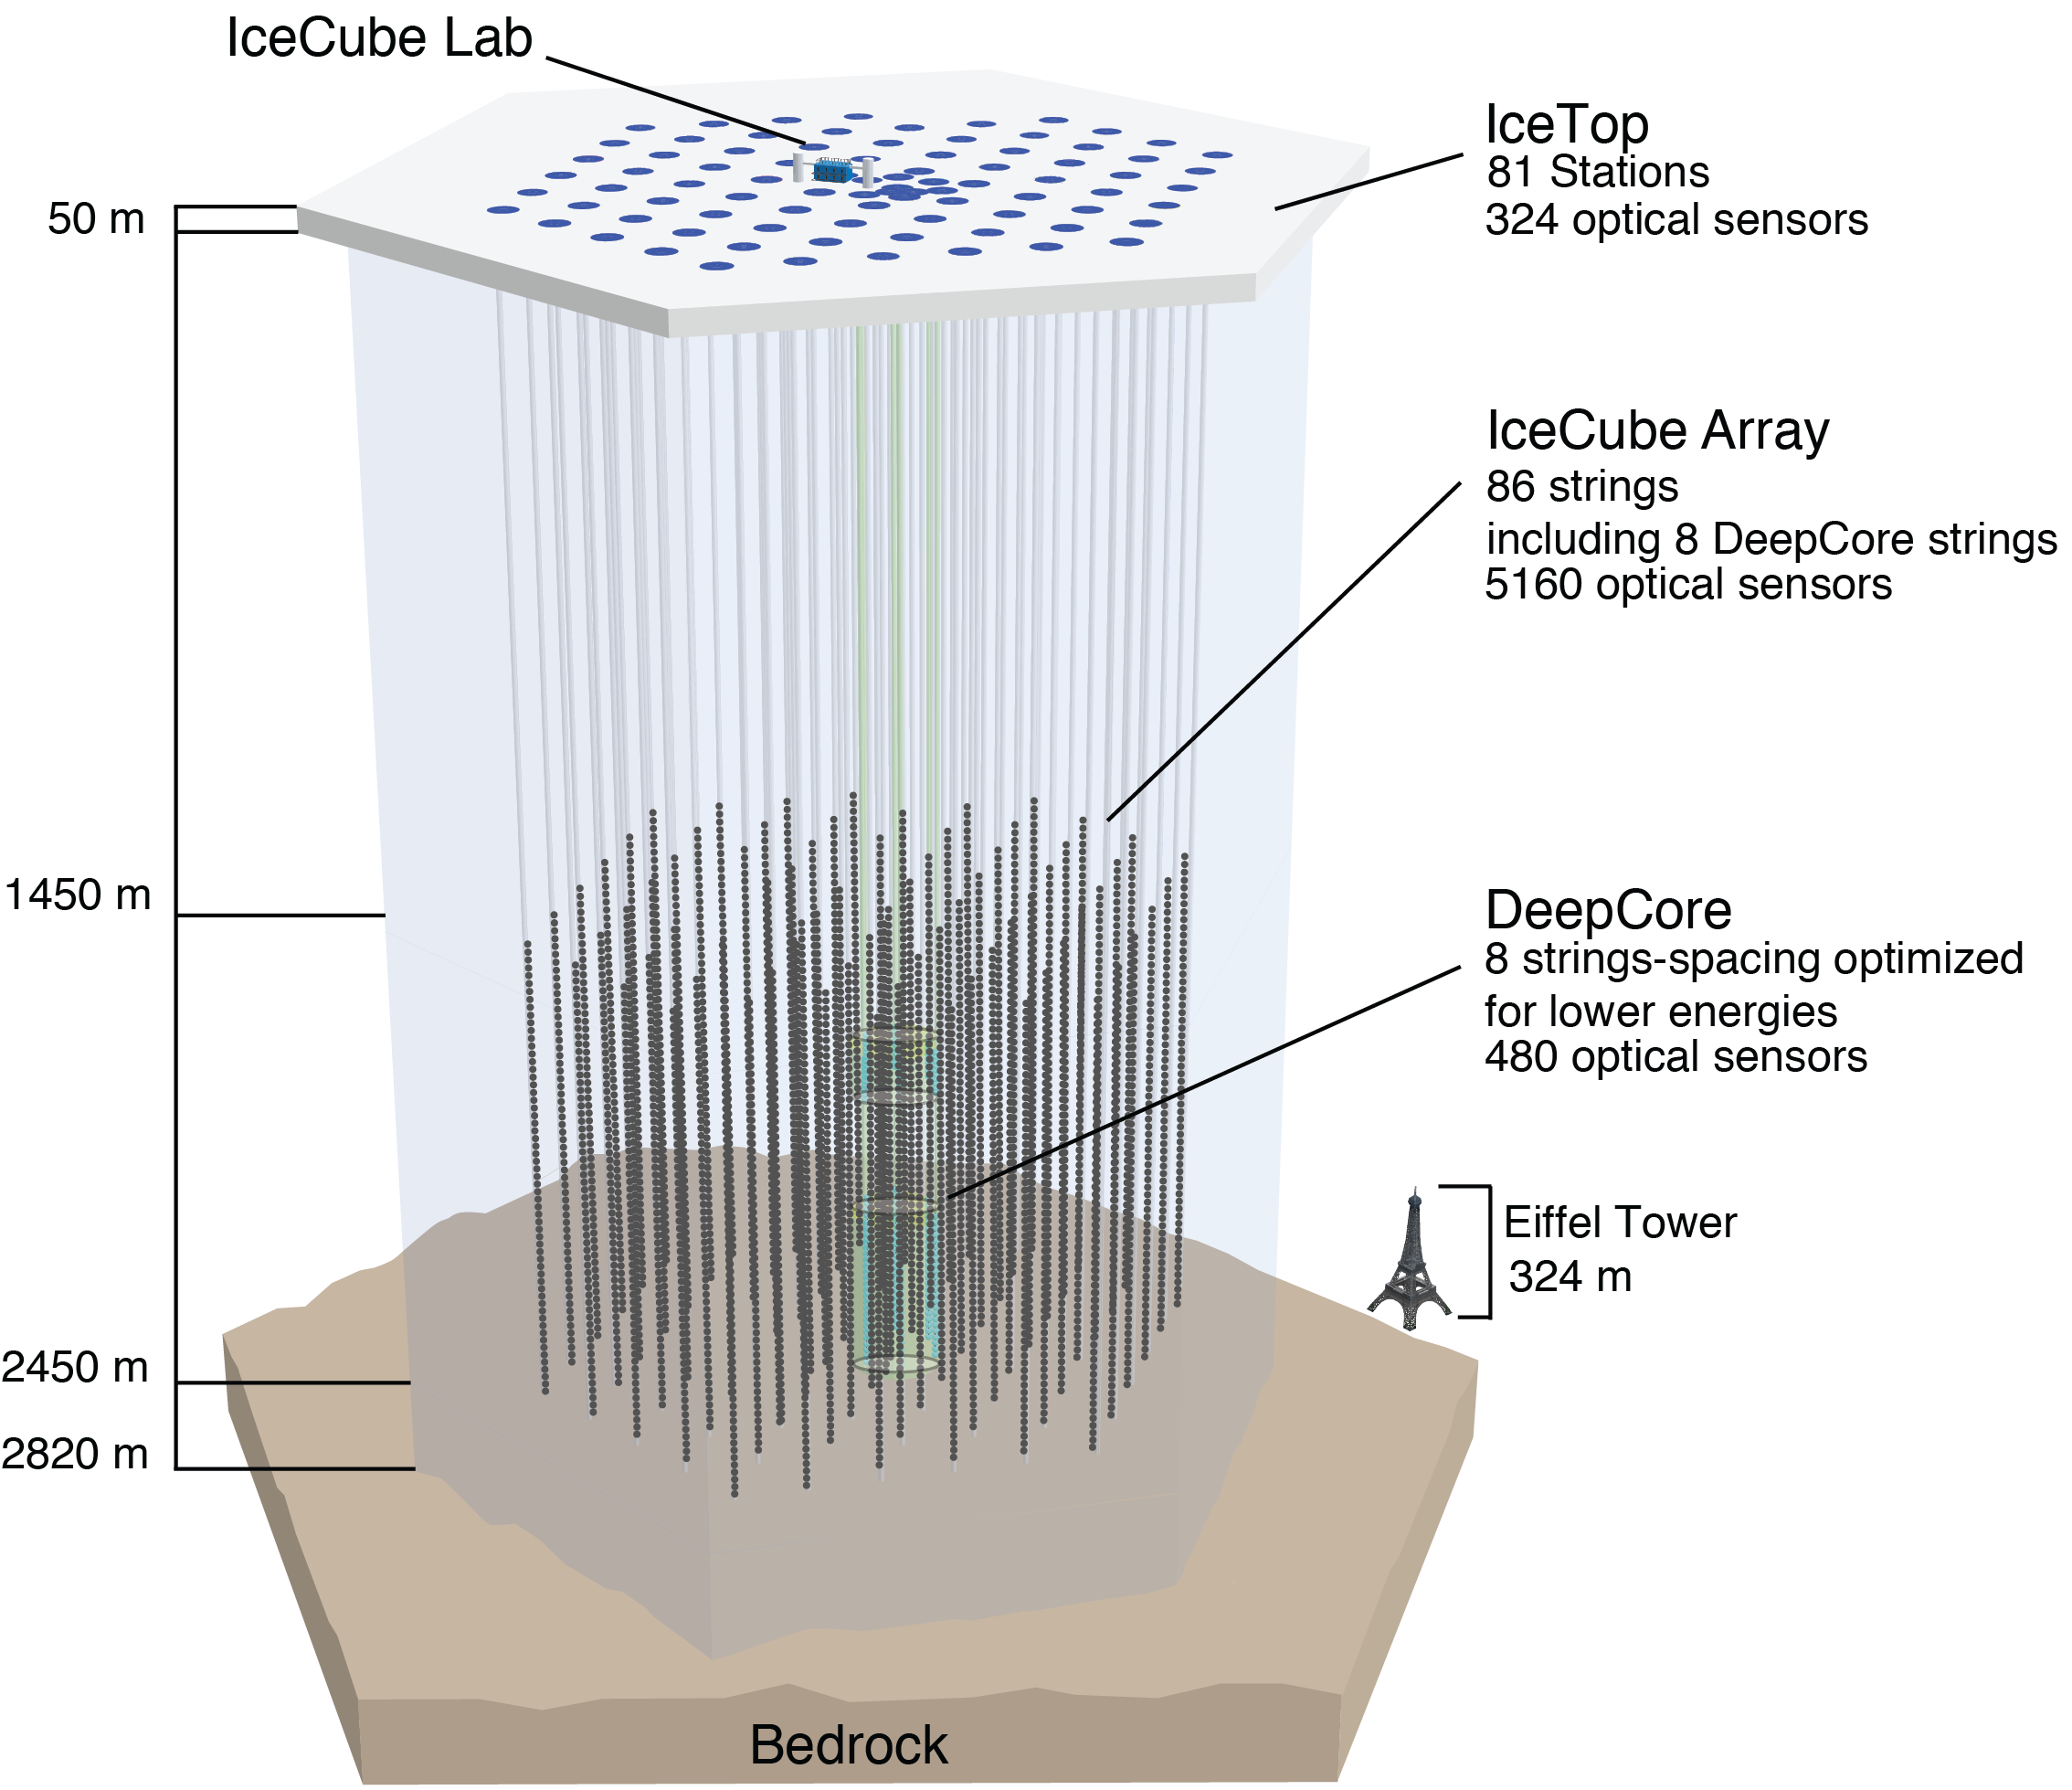
\includegraphics{figures/icecube_deepcore/IceCubeArray_slim.png}
	\caption[IceCube overview]{Overview of the IceCube detector showing the in-ice main- and sub-array IceCube and DeepCore, IceTop, and the IceCube Laboratory. From \cite{2017JInst..12P3012A_Instrumentation_Systems}.}
    \labfig{icecube_array}
\end{figure}

The full IceCube detector array consists of 86 vertical, in-ice strings and 81 surface stations as shown in \reffig{icecube_array}. The in-ice part is composed of 60 optical modules per string deployed at depths of \SIrange[range-phrase={~-~}]{1450}{2450}{\meter} below the ice, while the surface stations of the cosmic air-shower array, \textit{IceTop}, are ice-filled tanks. The surface stations and the majority of the strings are arranged in a hexagonal grid with the operations building, the \textit{IceCube Laboratory} (ICL), central to the grid on the surface. A top view of the hexagonal arrangement is shown in \reffig{icecube_top_view}. The in-ice array is designed to detect neutrinos in the energy range from \si{\giga\electronvolt} to \si{\peta\electronvolt}.


\subsection{Digital Optical Modules and the Antarctic Ice} \labsec{ice_and_DOMs}

The IceCube detection medium is the Antarctic glacial ice itself, which was formed over \SI{100000}{years} by accumulation of snow that was subsequently compressed by its own weight to form a dense crystal structure \sidecite{glacial_ice}. As a result of this formation process, the optical properties, scattering and absorption\todo{SB:
there are more properties than just these. Somehow need a half sentence that explains why these are particularly important to single out (see ice papers for inspiration) (ORANGE)
}, primarily change with depth. Within the detector volume the absorption length ranges from \SIrange[range-phrase={~-~}]{100}{400}{\meter}, while the scattering length lies between \SIrange[range-phrase={~and~}]{20}{100}{\meter}\todo{CL:
maybe define that absorption and scattering lengths are? they are defined differently so this invites a comparison that is not so obvious (ORANGE)
}. They are correlated, with the absorption length being roughly four times the scattering length \sidecite{ice_calibration}. The vertical distribution of scattering and absorption length can be seen in \reffig{ic_dc_sidecut}, where one dominant feature is the \textit{dust layer} between \SIrange[range-phrase={~and~}]{2000}{2100}{\meter} depth. This region has a higher concentration of dust particles that were deposited in a period of high volcanic activity, which leads to bad optical properties in form of larger scattering and absorption.\todo{Add reference for the dust layer! Maybe also from the ice paper? mention/cite dust logger paper/procedure? (ORANGE)}


\begin{figure}[h]
    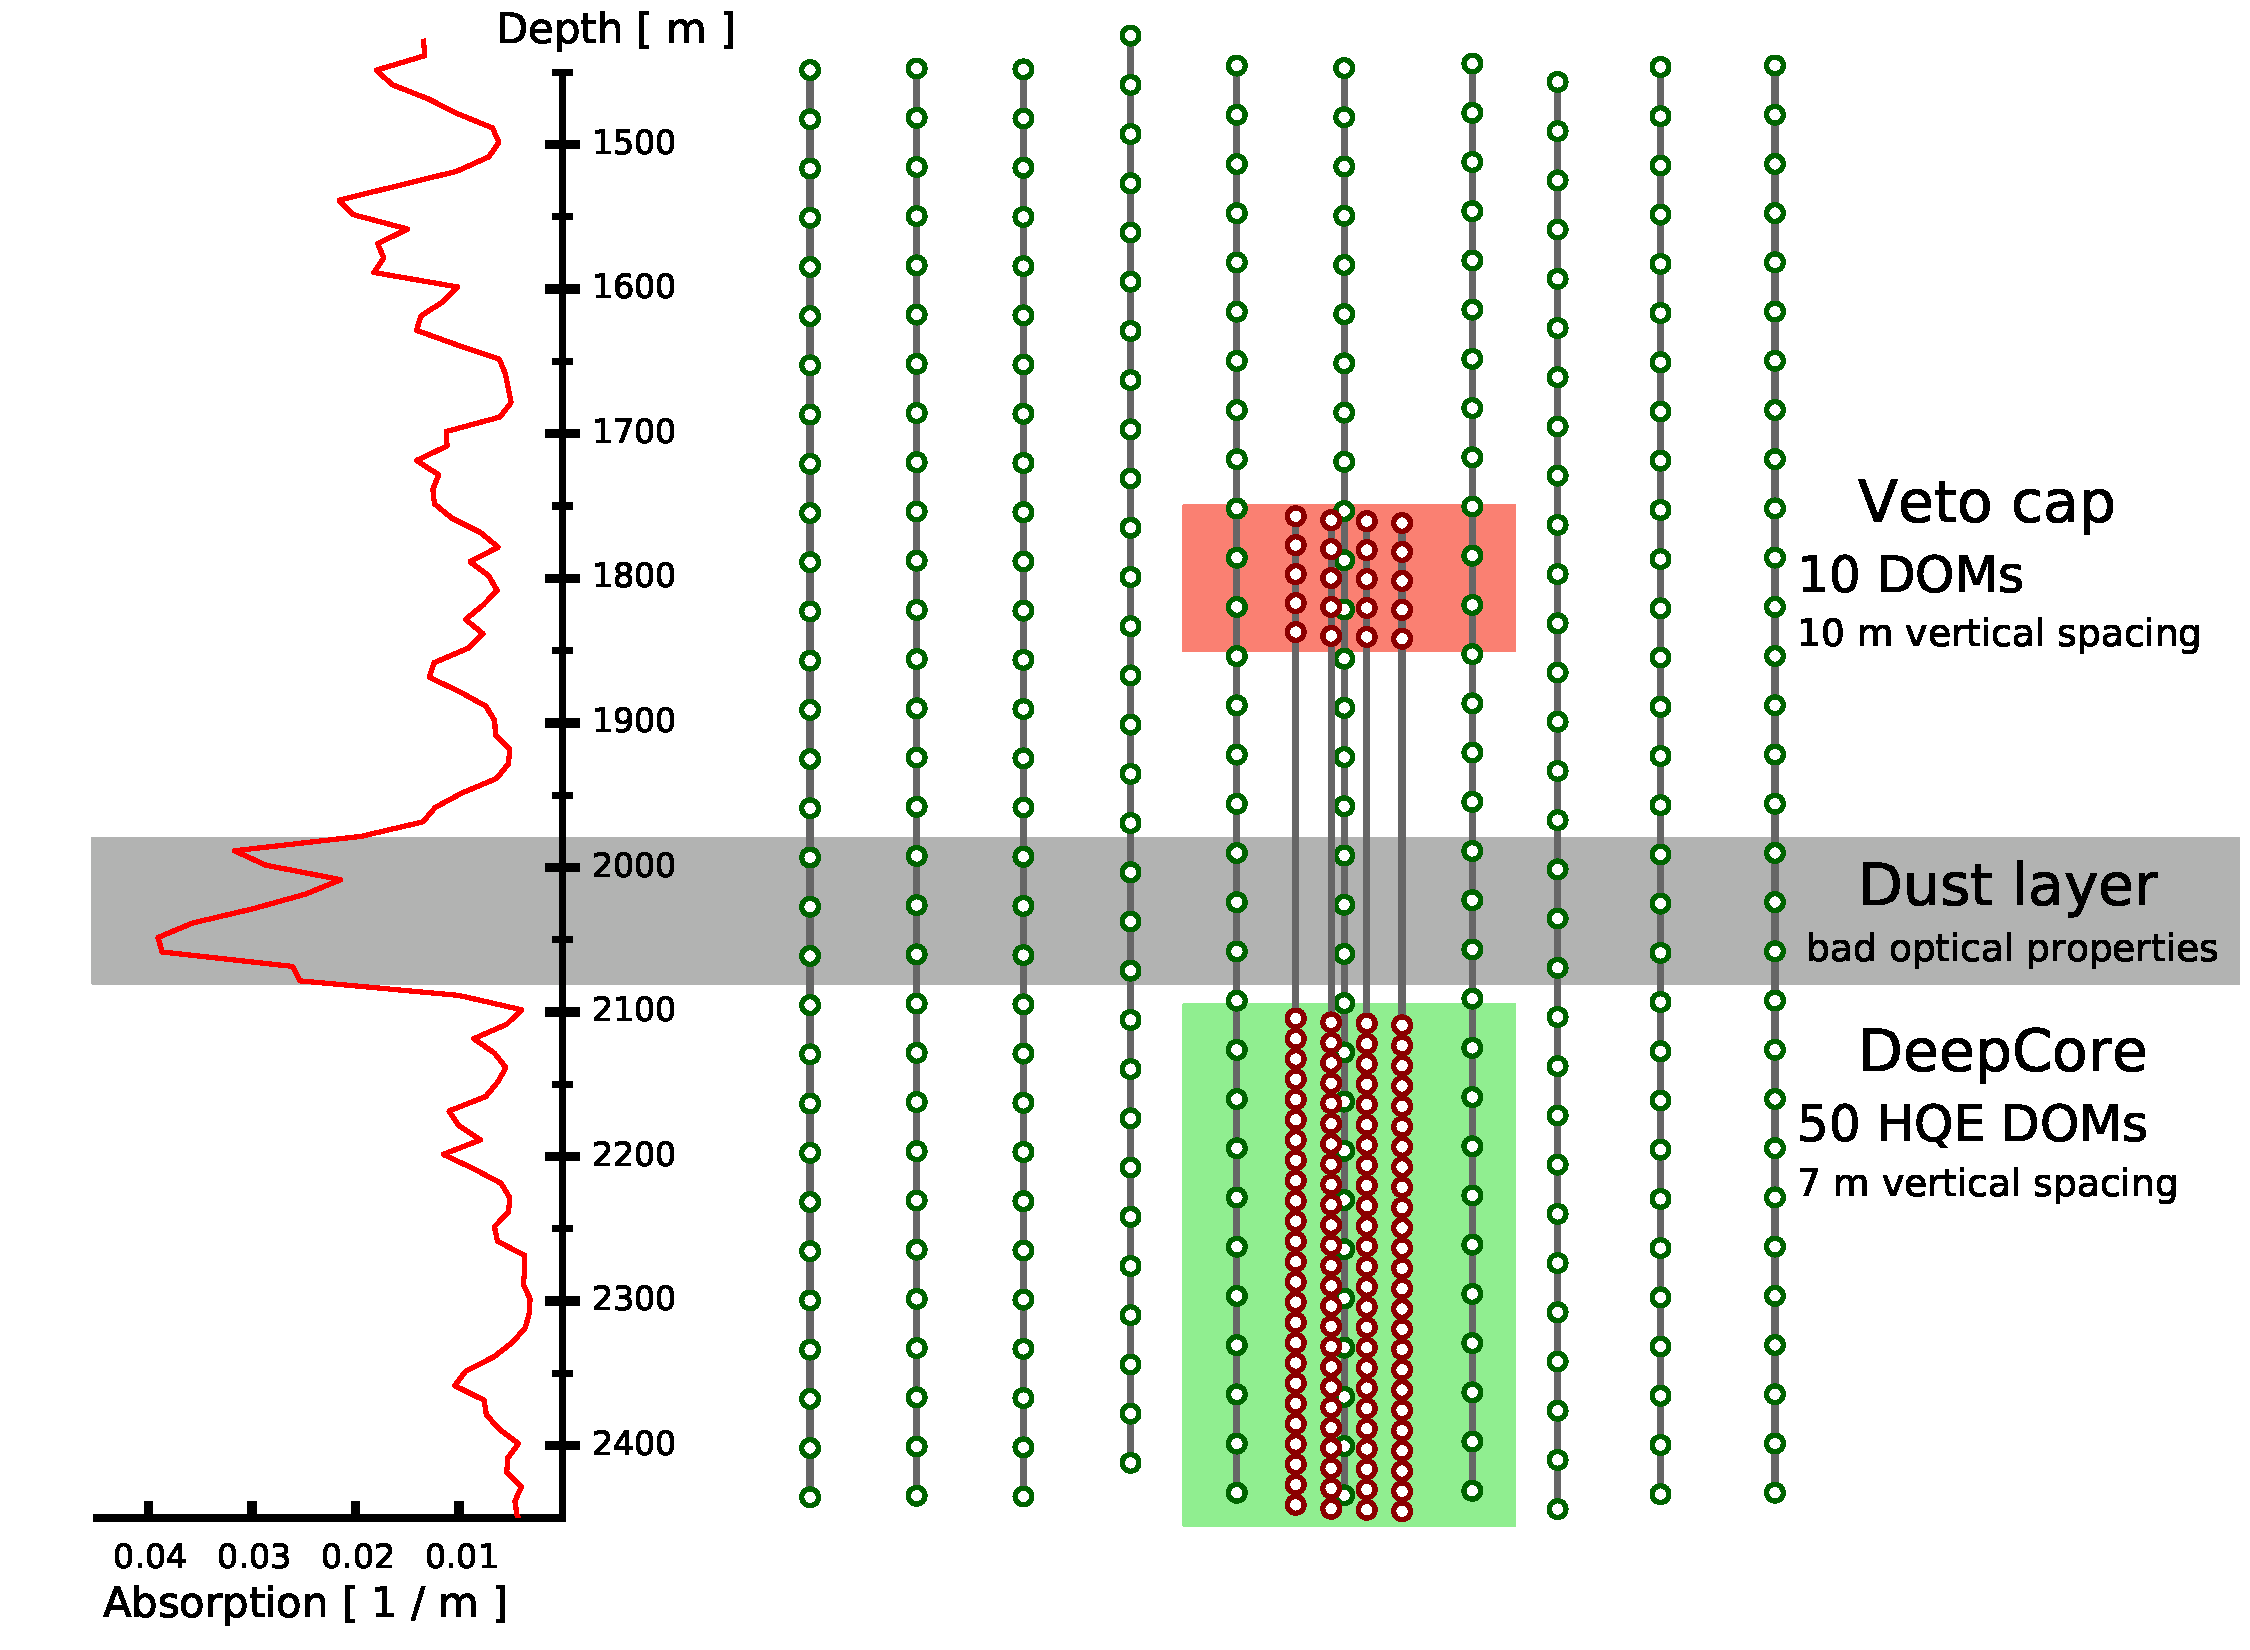
\includegraphics{figures/icecube_deepcore/DeepCore_sideview.pdf}
	\caption[IceCube side view]{Side view of IceCube and DeepCore showing the depth dependent scattering and absorption length (left panel) and the DOM positions around the dust layer.}
    \labfig{ic_dc_sidecut}
\end{figure}

\todo{exchange for figure with scattering (check abs/sca is correct) (ORANGE)}

The ice is instrumented by 5160 optical sensors called \textit{digital optical modules} (DOMs) \sidecite{ABBASI2009294_data_acquisition}, which can detect the Cherenkov light produced by charged particles traveling through the ice. Each DOM is made of a spherical glass housing, containing a downward-facing Photomultiplier Tube (PMT), the main-board with control, readout, and processing-electronics, and a LED flasher-board for calibration purposes. The design and the individual components of a DOM can be seen in \reffig{DOM_design}.

The majority of PMTs are the \SI{10}{"} Hamamatsu R7081-02, which have a bialkali photocathode and are sensitive to wavelengths in the range of \SIrange{300}{650}{\nano\meter}, with a peak quantum efficiency of 25\% at \SI{390}{\nano\meter}. In the central part of the IceCube array the peak efficiency reaches 34\%. The dark count rate in the temperature range of \SIrange{-40}{-20}{\degreeCelsius} is $\sim$\SI{300}{\hertz}. The DOM electronics measure the PMT voltage and control the gain. At a voltage crossing of the equivalent to \SI{0.25}{PE} the waveform readout is activated \sidecite{ABBASI2009294_data_acquisition}. Only when either one of the nearest or next to nearest DOMs above or below also sees a voltage crossing within a \SI{1}{\micro\second} time window \sidenote{This is referred to as a \textit{hard local coincidence (HLC)} \cite{ABBASI2009294_data_acquisition}.}, the voltages are digitized and sent to the ICL. Through the application of a waveform unfolding algorithm, called \textit{WaveDeform} \sidecite{IceCube:2013dkx}, the waveforms are compressed, and the results are the reconstructed times and charges of the photo-electrons. This is the basis for all further IceCube data processing.

\begin{marginfigure}
    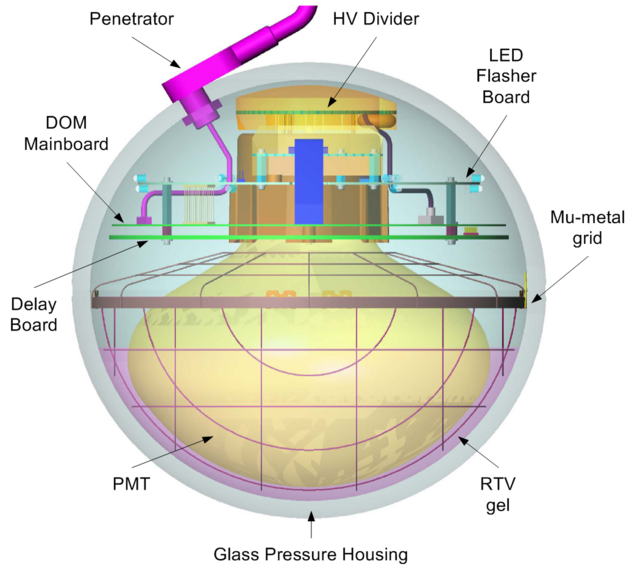
\includegraphics{figures/icecube_deepcore/DOM_schematic.png}
	\caption[Digital optical module (DOM)]{Design and components of a digital optical module (DOM) \cite{ABBASI2009294_data_acquisition}}
    \labfig{DOM_design}
\end{marginfigure}

The PMT is covered with a mu-metal grid (made from wire mesh), shielding the photocathode from Earth's magnetic field, and it is optically coupled to the glass sphere by RTV silicone gel. The glass sphere is a pressure vessel, designed to withstand both the constant ice pressure and the temporary pressure during the refreezing process of the water in the drill hole during deployment (peaking at around \SI{690}{\bar}). The sphere is held by a harness that connects the DOMs along a string and also guides the cable beside them.

The flasher-board controls 12 LEDs that produce optical pulses with a wavelength of \SI{405}{\nano\meter} \sidecite{2017JInst..12P3012A_Instrumentation_Systems}. The LEDs can be pulsed separately or in combination with variable output levels and pulse lengths. Using the known information of the light source positions and times this can be used for in-situ calibration of the detector by measuring absorption and scattering properties of the ice. Calibrating the absolute efficiency of the DOMs itself is more accurately done using minimum ionizing muons \sidecite{JFeintzeig_phd, domeff_nick}, since the total amplitude of the LED light is not well known.\todo{Add accuracy of the efficiency calibration here. (ORANGE)}


\subsection{IceCube Main-Array} \labsec{icecube}

\begin{figure}
    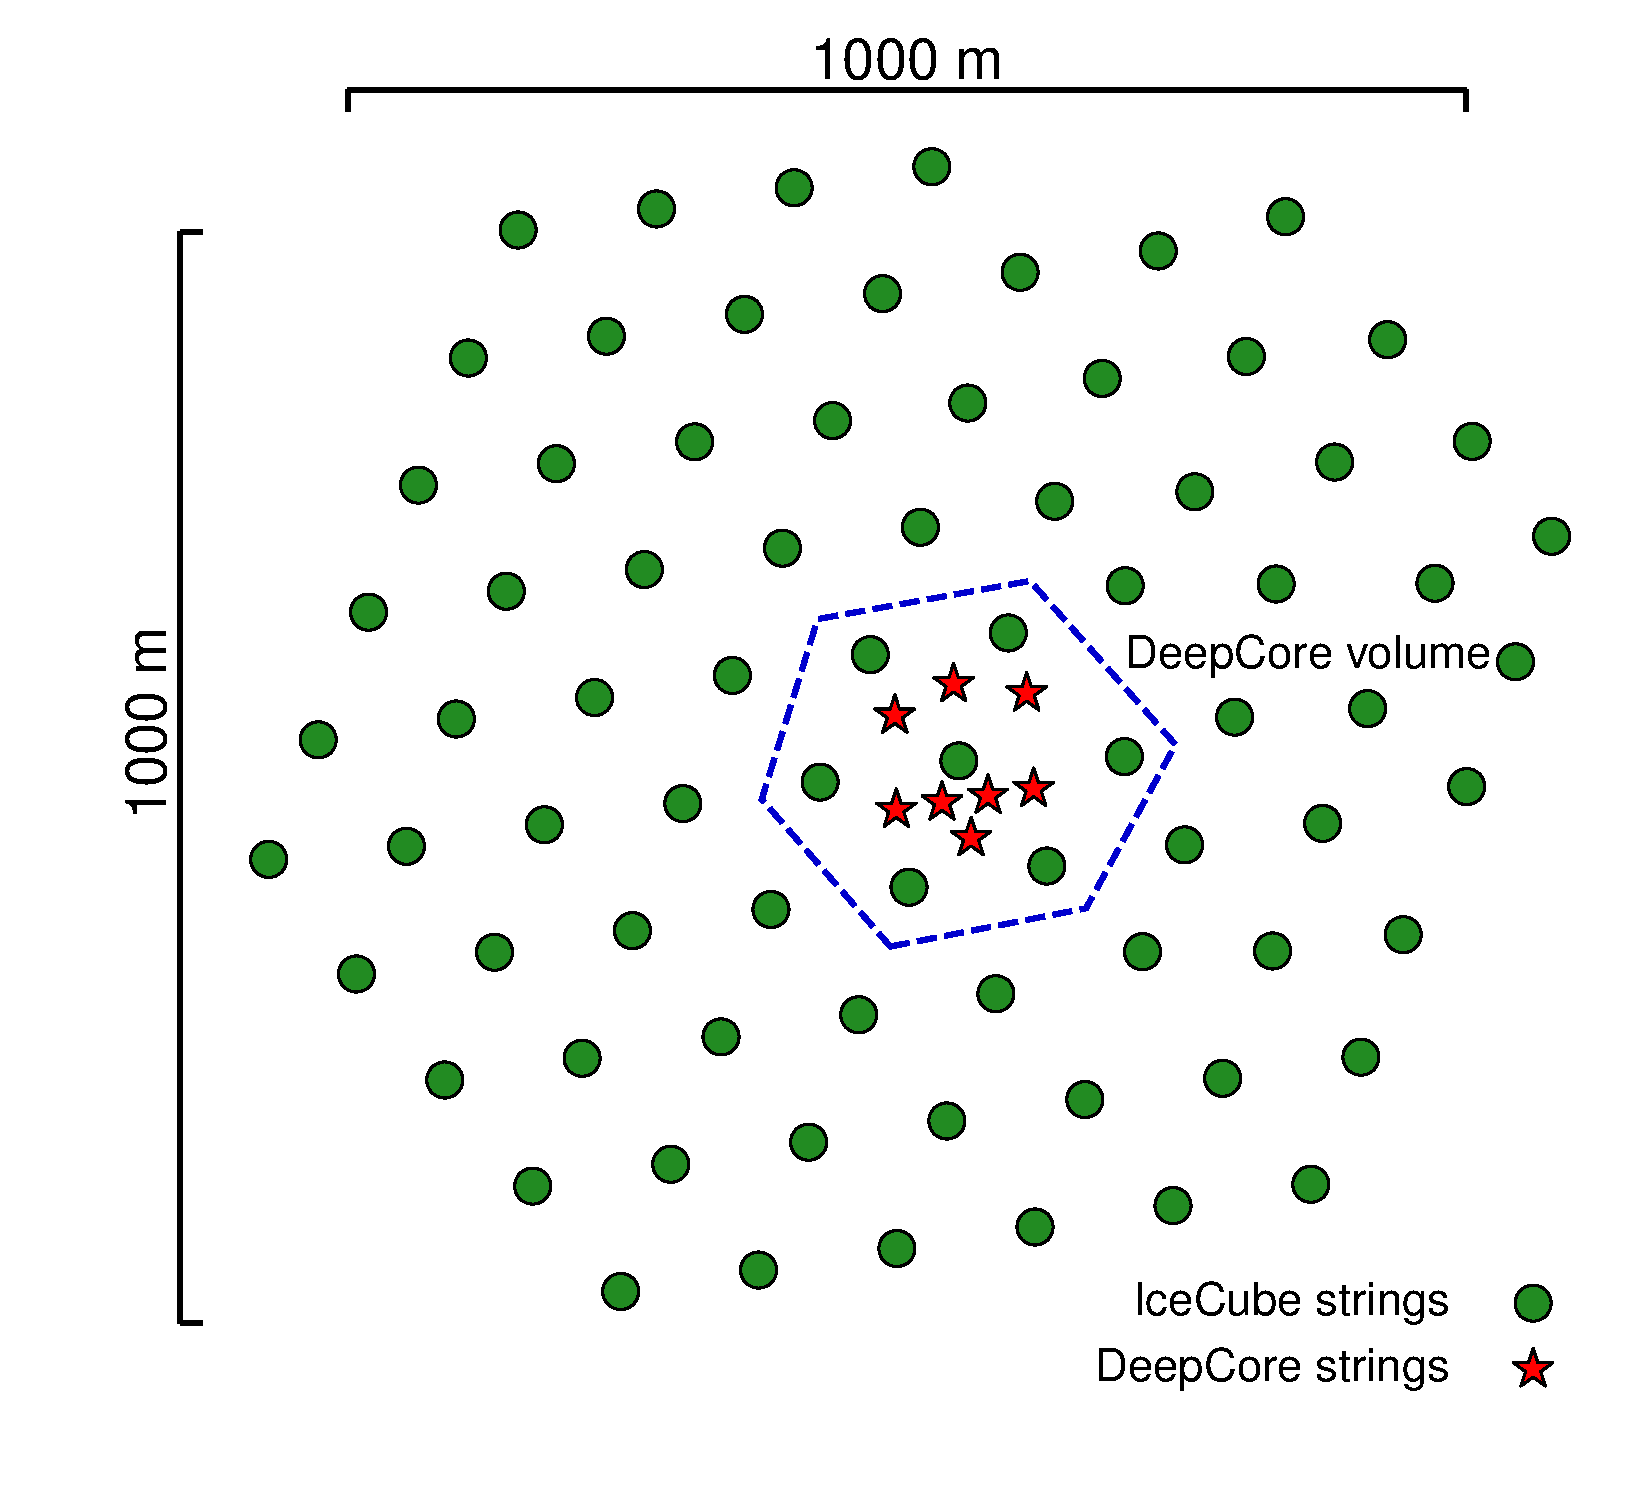
\includegraphics[trim={2.0cm, 1.5cm, 0, 0}, clip, width=0.65\linewidth]{figures/icecube_deepcore/icecube_top_view_bw.pdf}
    % 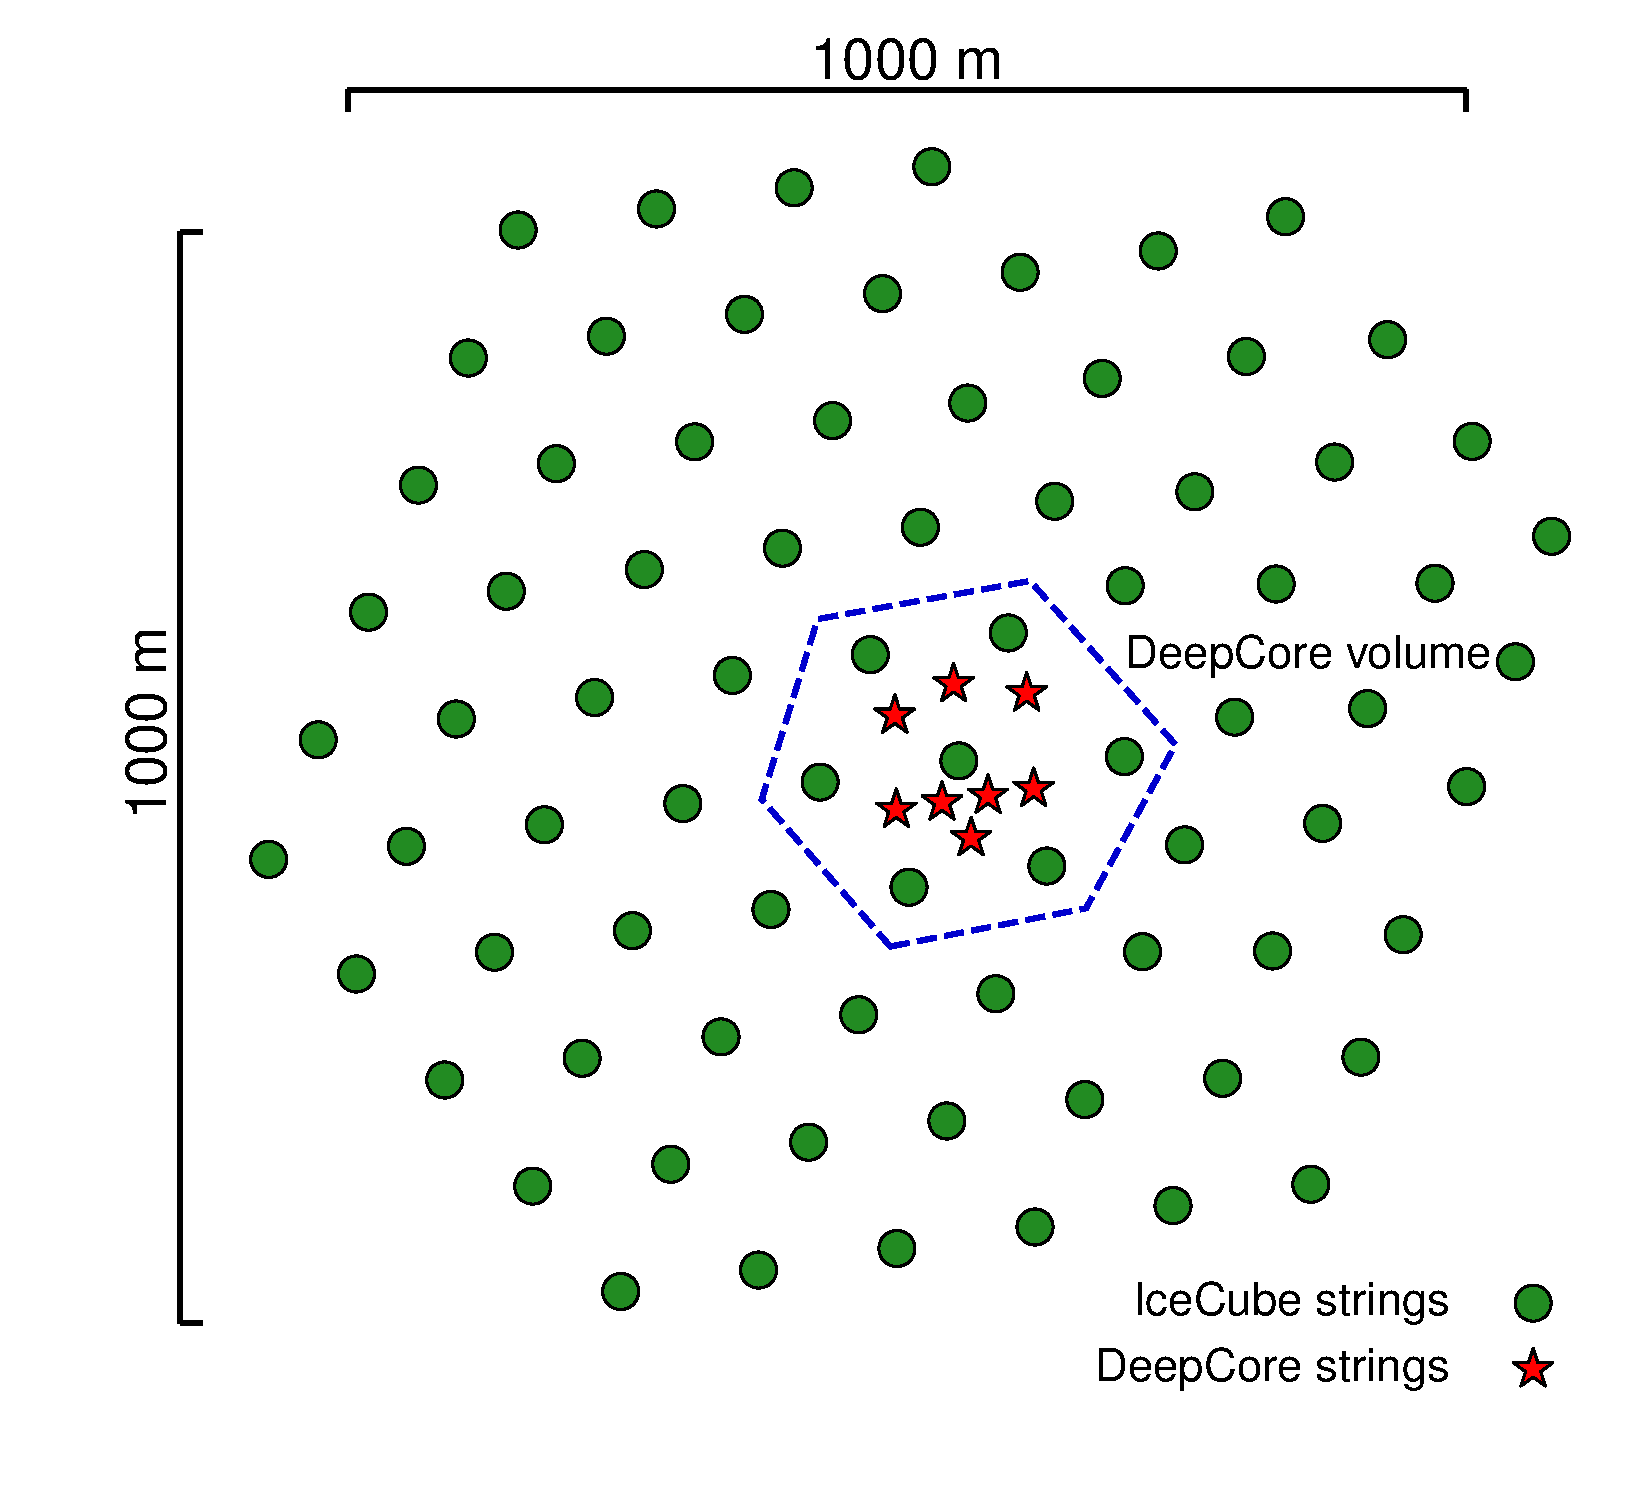
\includegraphics[trim={2.0cm, 1.5cm, 0, 0}, clip, width=1.0\linewidth]{figures/icecube_deepcore/icecube_top_view_bw.pdf}
    \caption[IceCube top view]{Top view of the IceCube array.}
    \labfig{icecube_top_view}
\end{figure}

The 78 strings that are arranged in a hexagonal pattern from the main part of the in-ice array, which is called \textit{IceCube}. With a $\sim$\SI{125}{\meter} horizontal spacing between the strings and a $\sim$\SI{17}{\meter} vertical spacing between DOMs, IceCube has a lower energy threshold of around \SI{100}{\gev}. IceCube was designed to detect astrophysical neutrinos with energies above \SI{1}{\tera\electronvolt}.

The coordinate system that is used in IceCube is centered at 46500'E, 52200'N at an elevation of \SI{883.9}{\meter} \sidecite{2017JInst..12P3012A_Instrumentation_Systems}. Per definition, it's a right-handed coordinate system where the y-axis points along the Prime Meridian (Grid North) towards Greenwich, UK, and the x-axis points \SI{90}{\degree} clockwise from the y-axis (Grid East). The z-axis is normal to the ice surface, pointing upwards. For IceCube analyses depth is defined as the distance along the z axis from the ice surface, assumed to be at an elevation of \SI{2832}{\meter}.


\subsection{DeepCore Sub-Array} \labsec{deepcore}

The additional 8 strings form a denser sub-array of IceCube called \textit{DeepCore} \sidecite{DeepCore_design_Abbasi2012615}. It is located at the bottom-center of the in-ice array and its \textit{fiducial volume} also includes the 7 surrounding IceCube strings as shown in \reffig{icecube_top_view}. The strings in this region have a closer average horizontal distance of about \SI{70}{\meter}. The lower 50 DeepCore DOMs on each string are placed in the region of clear ice below the dust layer between \SIrange{2100}{2450}{\meter} depth, where their vertical spacing is $\sim$\SI{7}{\meter}. The remaining 10 modules on each string are placed above the dust layer to be used as veto against atmospheric muons as can be seen in \reffig{ic_dc_sidecut}. Additionally, the DeepCore DOMs are equipped with higher quantum efficiency PMTs\sidenote{At \SI{400}{\nano\meter} they are \SI{35}{\percent} more efficient than the IceCube PMTs \cite{DeepCore_design_Abbasi2012615}.}. The combination of the denser spacing, the high quantum efficiency modules, and the most favorable ice properties below the dust layer leads to a lower energy detection threshold of around \SI{5}{GeV}, allowing the more efficient observation of atmospheric neutrinos.
, which are mostly in the energy range of \SIrange[range-phrase={~-~}]{10}{100}{\giga\electronvolt}.
Atmospheric neutrino oscillation analyses result in competitive measurements of the neutrino mixing parameters \sidecite{OVS_PRD, flercnn_analysis_result}, but the large flux of atmospheric neutrinos allows for many BSM searches, such as searches for dark matter, non-standard interactions, or sterile neutrinos.


\section{Particle Propagation in Ice} \labsec{icecube_propagation}

Neutrinos interacting in the ice via DIS produce muons, electromagnetic showers, and hadronic showers, depending on their flavor and the interaction type. The particles produced in those processes mainly lose their energy through \textit{ionization}, \textit{bremsstrahlung}, \textit{pair production}, and the \textit{photo-nuclear interaction}. Electrically charged particles also emit Cherenkov light when traveling through the ice, which is the main observable in IceCube, but only contributes a small amount to the total energy loss. The Cherenkov effect and the energy losses of the particles are described in the following sections, followed by an overview of the different particle signatures in IceCube.


\subsection{Cherenkov Effect} \labsec{cherenkov_effect}

When a charged particle moves through a medium with a velocity that is greater than the speed of light in that medium, it emits Cherenkov radiation.
% , losing a very small amount of energy ($\mathcal{O}$($10^{-4}$) of the total energy loss).
The detection principle of IceCube DeepCore, is based on the observation of resulting Cherenkov photons that are emitted by the charged secondary particles produced in the neutrino interactions that were introduced in \refsec{neutrino_interactions}. The Cherenkov effect was first observed by Pavel Cherenkov in 1934 \sidecite{CherenkovPhysRev.52.378} and occurs when the charged particle travels faster than the phase velocity of light, therefore polarizing the medium. Upon de-excitation the molecules emit the received energy as photons in a spherical wavefront. Since the particle moves past this wavefront, the superposition of the spherical light emissions forms a cone, which is shown in blue in the bottom panel of \reffig{cherenkov_light_front}.

\begin{marginfigure}
    \centering
    \begin{tikzpicture}[scale=0.6]

        % slower than speed of light
        \draw[draw=none,fill=gray!60] (10,8) circle (0.1);
        \draw[draw=none,fill=gray!60] (10.5,8) circle (0.1);
        \draw[draw=none,fill=gray!60] (11,8) circle (0.1);
        \draw[draw=none,fill=gray!60] (11.5,8) circle (0.1);
        \draw[draw=none,fill=gray!60] (11.7,8) circle (0.1);
            
        \draw[blue, line width=0.3mm] (10,8) circle (3.5);
        \draw[line width=0.3mm] (10.25,8) circle (3);
        \draw[line width=0.3mm] (10.5,8) circle (2.5);
        \draw[line width=0.3mm] (10.75,8) circle (2);
        \draw[line width=0.3mm] (11,8) circle (1.5);
        \draw[line width=0.3mm] (11.25,8) circle (1);
        \draw[line width=0.3mm] (11.5,8) circle (0.5);
        \draw[line width=0.3mm] (11.7,8) circle (0.1);

        \draw[orange, line width=0.6mm] (10,8) -- (11.7,8);
        \draw[draw=none,fill=orange] (11.8,8) -- +(210:0.45cm)arc (210:150:0.45cm) -- cycle;

        \draw[orange, line width=0.6mm] (10,8) -- (11.9,11.00);

        \node[draw=orange,line width=0.3mm] at (10.8,7.5) {$vt$};
        \node[draw=orange,line width=0.3mm, rotate=59] at (10.5,9.7) {$ct$};

        \node[line width=0.3mm] at (10,4) {$v<c$};


        % faster than speed of light
        \draw[draw=none,fill=gray!60] (9,0) circle (0.1);
        \draw[draw=none,fill=gray!60] (10,0) circle (0.1);
        \draw[draw=none,fill=gray!60] (11,0) circle (0.1);
        \draw[draw=none,fill=gray!60] (12,0) circle (0.1);
        \draw[draw=none,fill=gray!60] (13,0) circle (0.1);
        \draw[draw=none,fill=gray!60] (13.5,0) circle (0.1);
        
        \draw[line width=0.3mm] (9,0) circle (2.5);
        \draw[line width=0.3mm] (10,0) circle (2);
        \draw[line width=0.3mm] (11,0) circle (1.5);
        \draw[line width=0.3mm] (12,0) circle (1);
        \draw[line width=0.3mm] (13,0) circle (0.5);
        \draw[line width=0.3mm] (13.5,0) circle (0.25);
        
        \draw[blue, line width=0.3mm] (8,3.45) -- (14,0);
        \draw[blue, line width=0.3mm] (8,-3.45) -- (14,0);
        
        \draw[orange, line width=0.6mm] (9,0) -- (14,0);
        \draw[draw=none,fill=orange] (14.1,0) -- +(210:0.45cm)arc (210:150:0.45cm) -- cycle;

        \draw[orange, line width=0.6mm] (9,0) -- (10.3,2.15);
        
        \draw[orange, line width=0.6mm] (9.8,0) arc (0:55:0.8cm);
        
        
        \node[] at (8.7,-0.6) {$\theta_c$};
        \draw[line width=0.2mm] (8.9,-0.4) -- (9.5,0.25);

        \node[draw=orange,line width=0.3mm] at (10.5,-0.5) {$vt$};
        \node[draw=orange,line width=0.3mm, rotate=59] at (9.0,1.0) {$ct$};

        \node[line width=0.3mm] at (10,-3.5) {$v>c$};

    \end{tikzpicture}
    \caption[Cherenkov light front]{Schematic depiction of the spherical light front produced by a particle traveling slower than the speed of light in the medium (top) and the formation of the Cherenkov light front produced by a charged particle traveling faster than the speed of light in the medium (bottom). Blue is the resulting wavefront, while the black circles are spherically emitted light at each position and the orange arrows show the direction of the particle.}
    \labfig{cherenkov_light_front}
\end{marginfigure}

Using trigonometry, the angle $\theta_c$ at which the Cherenkov light is emitted can be calculated as
\begin{equation}
    \theta_c = \arccos\Big(\frac{1}{\beta n}\Big)
    \;,
    \labeq{cherenkov_angle}
\end{equation}
where $\beta$ is the velocity of the particle in units of the speed of light and $n$ is the refractive index of the medium. When the particle velocity is close to the speed of light, the equation holds and the angle is only dependent on the refractive index of the medium. For the ice, the refractive index is $n \approx 1.3$ and as a result $\theta_c \approx 41^\circ$ \sidecite{physics_of_ice_10.1093/acprof:oso/9780198518945.003.0009}.

The frequency of the emission depends on the charge $z$ and the wavelength-dependent index of refraction $n(\omega)$ and is given by the Frank-Tamm formula \sidecite{frank, tamm}
\begin{equation}
    \frac{d^2N}{dxd\lambda} = \frac{2\pi\alpha z^2}{\lambda^2} \Big(1 - \frac{1}{\beta^2n(\omega)^2}\Big)
    \;,
    \labeq{frank_tamm}
\end{equation}
with $\alpha\approx1/137$ the fine structure constant, $\lambda$ the wavelength of the emitted light, and $x$ the path length traversed by the particle. Relativistic particles in ice produce roughly 250 photons per cm in the wavelength range of \SIrange[range-phrase={~-~}]{300}{500}{\nano\meter} \sidecite{raedel_wiebusch_cherenkov_yield}.


\subsection{Energy Losses} \labsec{energy_loss}

Even though relativistic, charged particles traveling through matter produce Cherenkov radiation, their energy is mainly lost through other processes that are dependent on the particle type and energy. The exact principles of energy loss for the different types can broadly be categorized into the three groups: quasi-continuous energy loss by muons, electromagnetic cascades, and hadronic cascades.


\subsubsection{Muons}

Muons lose their energy by ionization, bremsstrahlung, pair production, and the photo-nuclear effect. The energy loss by ionization is the dominant process for muons above \SI{1}{\giga\electronvolt} and has a weak energy dependence given by \sidecite{PDG_review_2022}
\begin{equation}
    \Bigl \langle -\frac{\mathrm{d}E}{\mathrm{d}x} \Bigr \rangle = a_I(E) + b_R(E) \cdot E
    \;,
    \labeq{radiative_losses}
\end{equation}
where $E$ is the energy and $a_I(E)$ and $b_R(E) \cdot E$ are the energy loss by ionization and the combined radiative losses, respectively. In the energy range relevant for this work (\SIrange[range-phrase={~-~}]{10}{100}{\giga\electronvolt}), the parameters $a_I$ and $b_R$ only depend on energy very weakly and can be approximated by constants. The energy loss is then given by
\begin{equation}
    \Bigl \langle -\frac{\mathrm{d}E}{\mathrm{d}x} \Bigr \rangle = a + b \cdot E
    \;.
    \labeq{radiative_losses_simple}
\end{equation}
Based on this description, there is a critical energy which divides the regimes where ionization and radiative losses dominate. The critical energy is given by $E_\rm{crit} = a/b$ and for muons in ice it is $\sim$\SI{713}{\giga\electronvolt} (using $a \approx$ \SI{2.59}{\mega\electronvolt\cm^{-1}} and $b \approx$ \SI{3.63e-6}{\cm^{-1}} \sidecite{2004hep.ph....7075C}). Since the energy range of interest is well below this critical energy, the range of a muon can easily be related to its energy by
\begin{equation}
    \langle L \rangle = \frac{E_0}{a}
    \;.
    \labeq{muon_range_approx}
\end{equation}
Measuring the length of a muon track therefore allows for an estimation of its energy if the full track is contained within the instrumented volume of IceCube. Using the given numbers a \SI{30}{\giga\electronvolt} muon travels $\sim$\SI{116}{\meter}, which is well within the instrumented volume of IceCube, which spans across distances of up to \SI{1000}{\meter}. This approximate treatment does not take into account the stochastic nature of some energy losses. Bremsstrahlung and photo-nuclear interactions for example rarely occur, but when they do, they deposit a large chunk of energy. A thorough investigation of the energy losses of muons in ice can be found in \sidecite{LRaedel}.


\subsubsection{Electromagnetic Showers}

Photons as well as electrons and positrons are produced either directly in neutrino interactions or in secondary particle interactions. Above a critical energy $E_c$, they lose their energy through repeated pair production and bremsstrahlung emission forming an expanding, electromagnetic shower profile. The particles' energy reduces with every interaction and their number increases until they fall below the critical energy where ionization and excitation of surrounding atoms become the dominant energy loss processes for electrons and positrons. For photons the remaining energy is lost through the Compton effect and the photoelectric effect \sidecite{PDG_review_2022}. Below the critical energy no new shower particles are produced. Electromagnetic cascades can be characterized by the radiation length, $X_0$, after which electrons/positrons reduced their energy to $1/e$ of their initial energy. For photons, it's equivalent to $7/9$ of the mean free path of pair production. The critical energy for ice is $E_c \approx$ \SI{78}{\mega\electronvolt}, with a radiation length of $X_0 \approx$ \SI{39.3}{\centi\meter} \sidecite{PhysRevD.98.030001}.

The radiation length governs the longitudinal shower profile and using $t=x/X_{0}$, the shower intensity can be described by a gamma distribution \sidecite{em_gamma_distribution_Longo:1975wb, PDG_review_2022}
\begin{equation}
    \frac{dE}{dt} = E_0b \frac{({bt})^{a-1} e^{-bt}}{\Gamma(a)}
    \;,
    \labeq{gamma_distribution}
\end{equation}
where $a$ and $b$ are parameters that have to be estimated from experiment, and $E_0$ is the initial shower energy. Based on the work from \sidecite{LRaedel}, performed with \textsc{Geant4} \sidecite{geant4}, the parameters for electromagnetic showers in ice are
\begin{subequations}
    \begin{align}
        e^-: \; a \approx 2.01 + 1.45 \log_{10} (E_0/\si{\giga\electronvolt}),\; & b \approx 0.63 \;, \\
        e^+: \; a \approx 2.00 + 1.46 \log_{10} (E_0/\si{\giga\electronvolt}),\; & b \approx 0.63 \;, \\
        \gamma: \; a \approx 2.84 + 1.34 \log_{10} (E_0/\si{\giga\electronvolt}),\; & b \approx 0.65 \;.
        \labeq{gamma_distribution_parameter}
    \end{align}
\end{subequations}
The maximum of the shower is at $t_{max} = (a-1)/b$ and the Cherenkov emission of the charged particles produced in the shower is peaked around the Cherenkov angle, since they are produced in the forward direction.
\todo{Add angular profile plot (Summer agrees!) (create one based on Leif Rädel as Alex did) (RED)}


\subsubsection{Hadronic Showers}

In DIS interactions, a cascade is always produced by the hadrons coming from the breaking target nucleus. The cascade is a result of secondary particles produced in strong interactions between the hadrons and the traversed matter. The charged particles produced in the shower will emit Cherenkov radiation, while neutral particles will be invisible to the detector. There is also an electromagnetic component of the shower, due to for example the decay of neutral pions into photons. Hadronic showers of the same energy as electromagnetic showers have larger fluctuations in energy deposition and shape, since they depend on the produced particle types. Hadrons also have a higher energy threshold for Cherenkov light production, because of their higher mass. Based on \sidecite{GABRIEL1994336, LRaedel}, the visible electromagnetic fraction of hadronic showers can be parameterized as
\begin{equation}
    F(E_0) = \frac{T_\mathrm{hadron}}{T_\mathrm{EM}} = 1 - (1 - f_0)\Big(\frac{E_0}{E_s}\Big)^{-m}
    \;,
    \labeq{hadronic_shower_fraction}
\end{equation}
where $T_\mathrm{hadron/EM}$ is the total track length of a hadronic/electromagnetic shower with the same energy, $f_0$ is the ratio of hadronic and electromagnetic light yield, $E_0$ is the initial energy, and $E_s$ is an energy scale. The parameter $m$ is a free model parameter. The ratio $F(E_0)$ increases with energy, but is always smaller than $1$. The variance of this distribution is given by
\begin{equation}
    \sigma_F(E_0) = \sigma_0 \log(E_0)^{-\gamma}
    \;.
    \labeq{hadronic_shower_fraction_variance}
\end{equation}
The parameters $m$, $E_s$, and $f_0$ were estimated by fitting the model to the results of Geant4 simulations. Cherenkov light from hadronic showers also peaks around the Cherenkov angle, but the angular distribution is more smeared out, due to the variations in particle type and their energy depositions.


\section{Event Morphologies} \labsec{icecube_signatures}

The event morphologies produced by particles detected in IceCube are combinations of the three energy loss types described in \refsec{energy_loss}, e.g. \textit{cascades} from electromagnetic and hadronic showers and elongated \textit{tracks} from muons traveling through the detector. \reftab{interactions_vs_signatures} gives an overview of the possible event signatures.

\begin{table}[h]
    \small
    \begin{center}
        \begin{tabular}{ m{1.8cm} m{2.0cm} m{3.0cm} m{1.8cm} }
        % \begin{tabular}{ l l l l }

            \hline\hline

            \textbf{Interaction} & \multicolumn{2}{c}{\textbf{Secondary particles}} &\textbf{Signature} \\

            \hline\hline

            \multirow{2}{*}[-1.5em]{CC $\overset{(-)}{\nu_\mu}$ }
            & 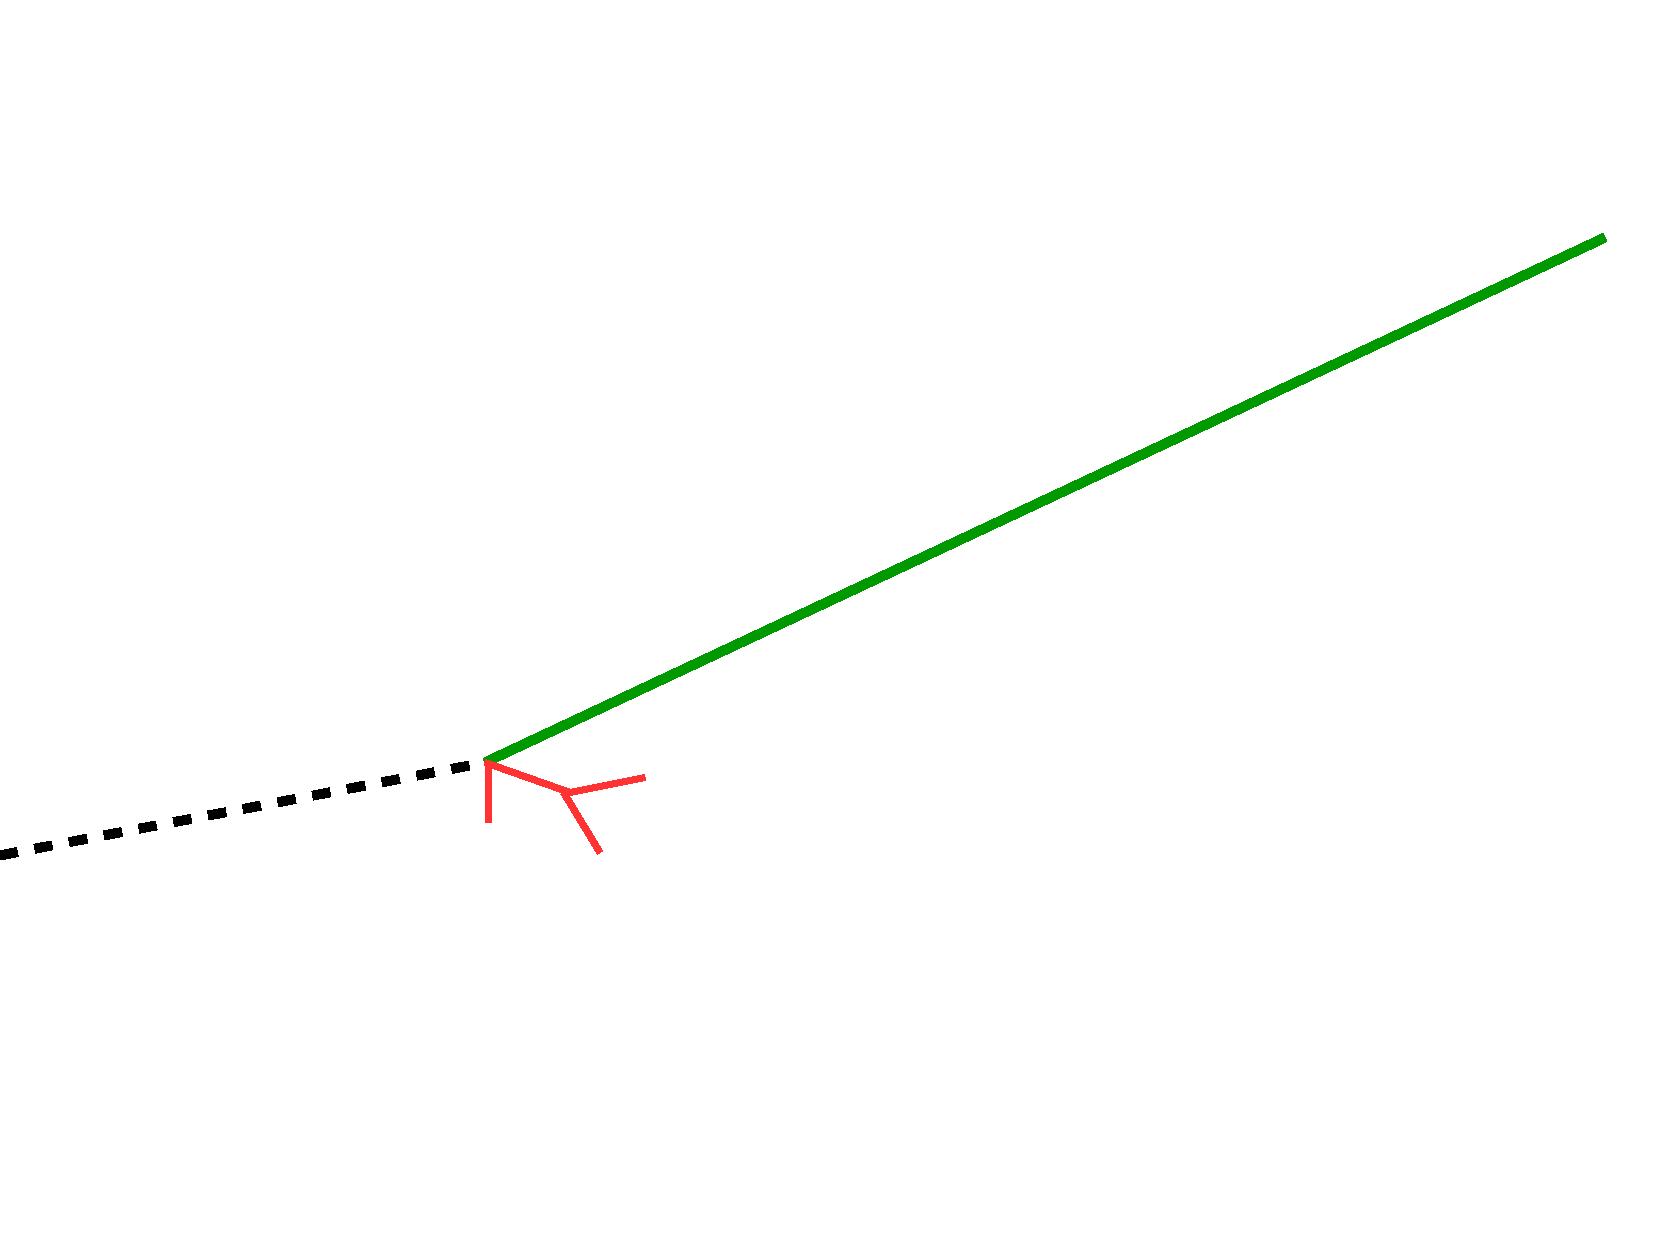
\includegraphics[width=2cm]{figures/neutrinos_properties/interaction_schematics/numu_CC_muon_only.pdf} 
            & $\mu^\pm$ track 
            & Track-only \\

            \cmidrule{2-4} 
            &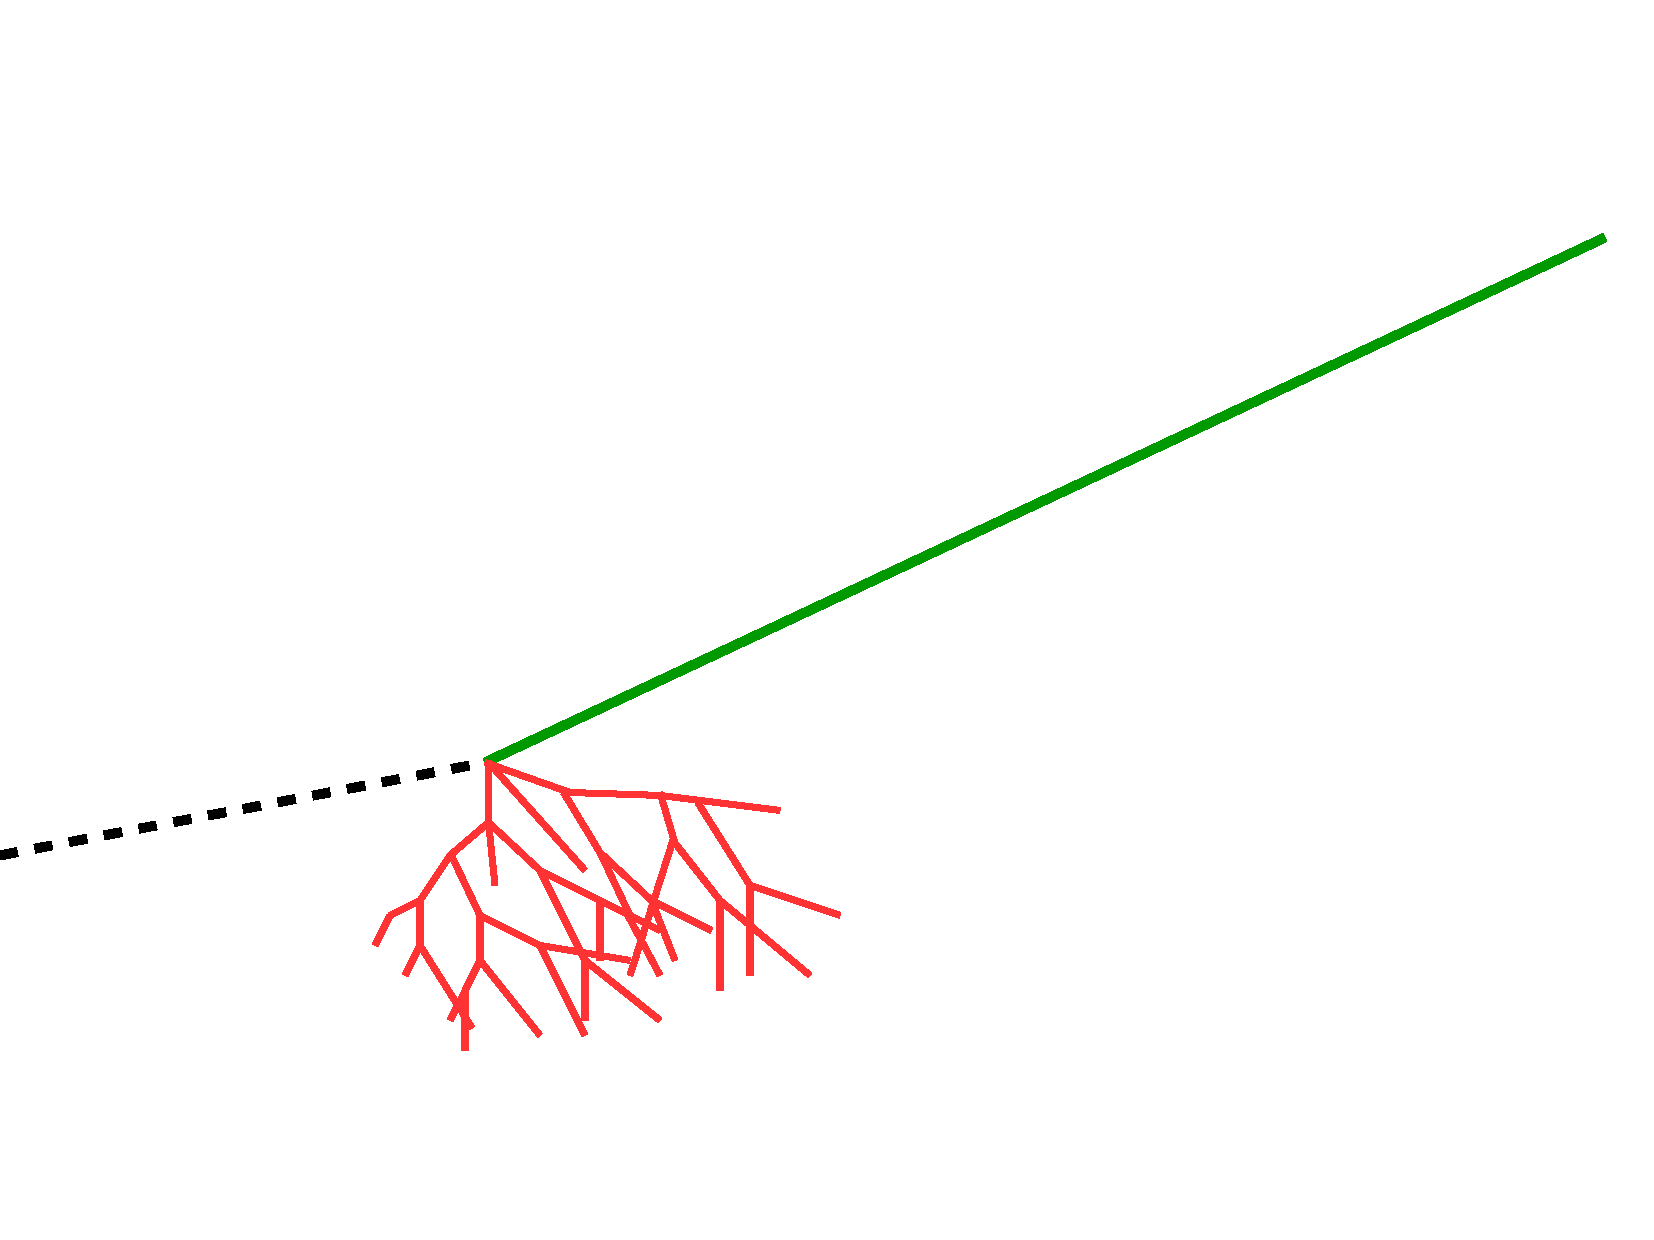
\includegraphics[width=2cm]{figures/neutrinos_properties/interaction_schematics/numu_CC_track_cascade.pdf}  
            & $\mu^\pm$ track and hadrons 
            & \multirow{2}{*}[-1.3em] {Cascade + track} \\

            \cmidrule{1-3}

            \multirow{2}{*}[-1.5em]{CC $\overset{(-)}{\nu_\tau}$ }
            &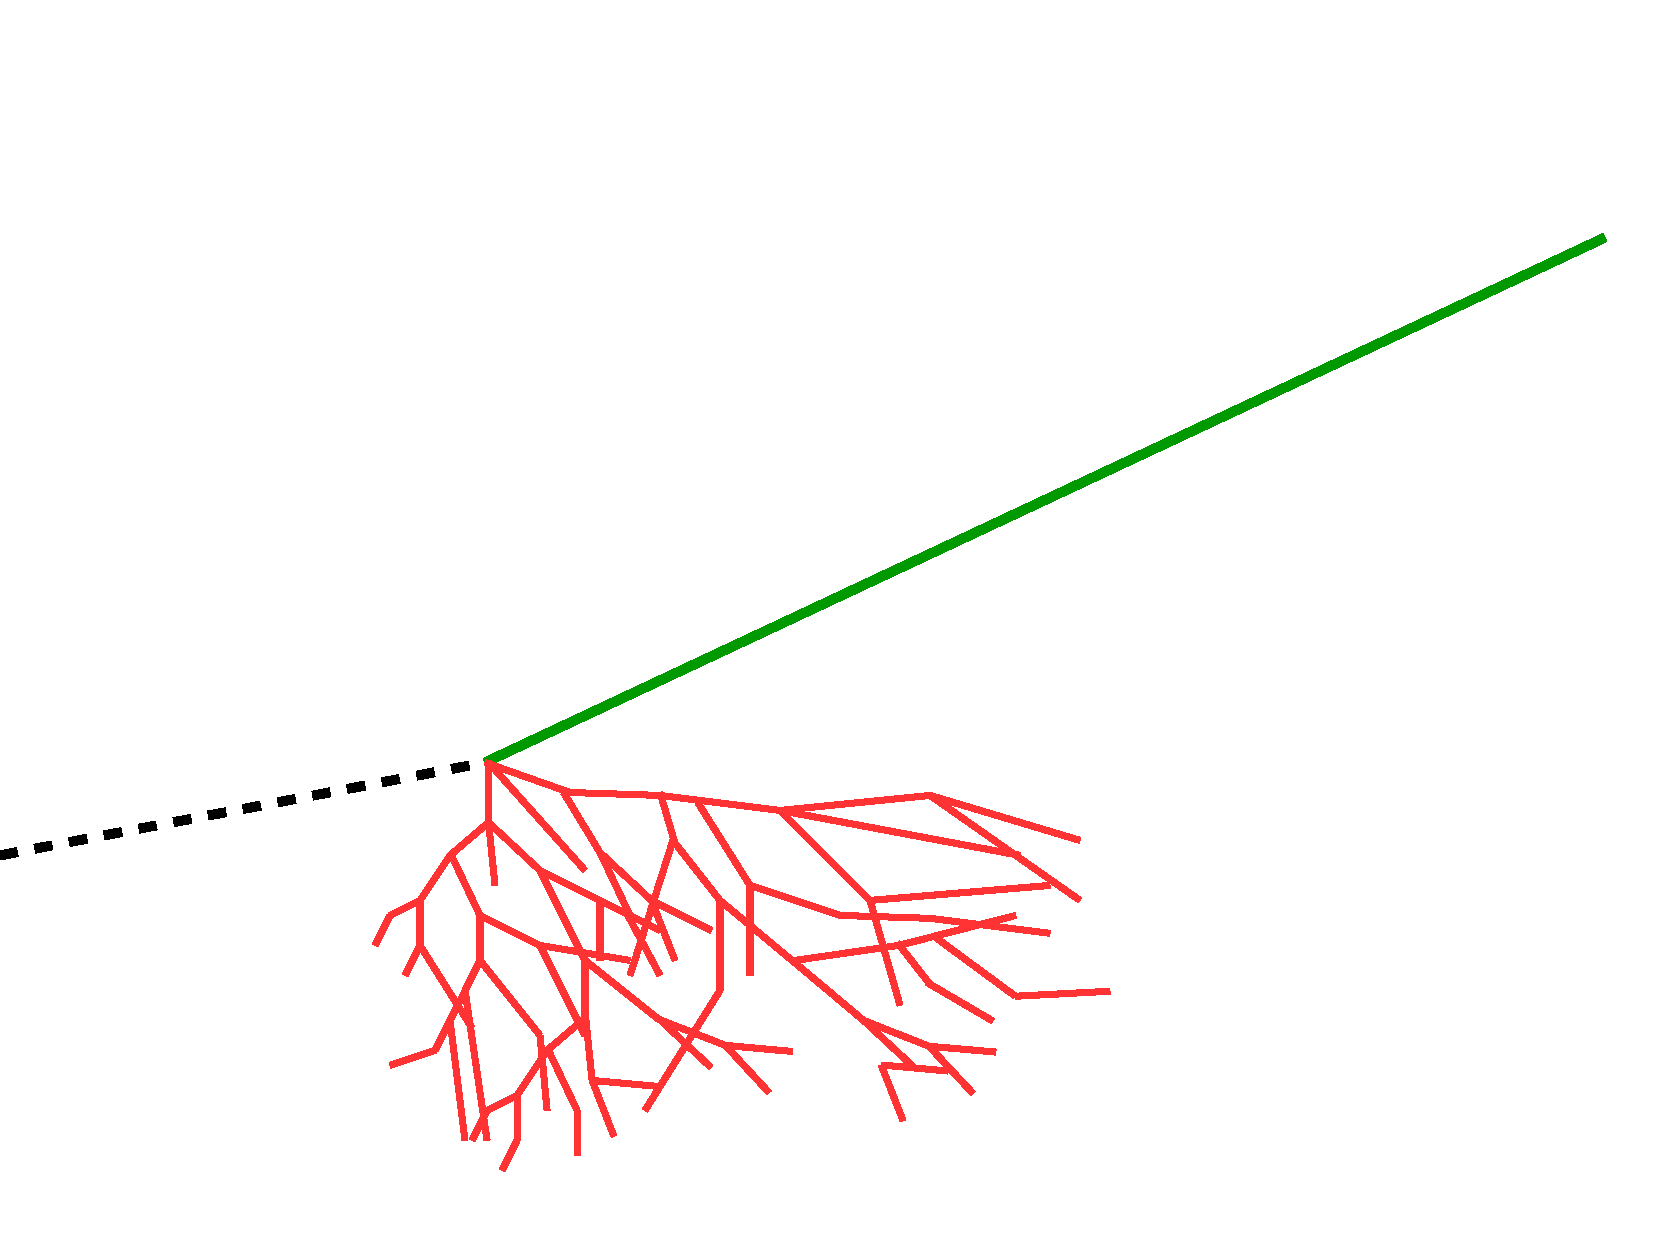
\includegraphics[width=2cm]{figures/neutrinos_properties/interaction_schematics/nutau_CC_track_cascade.pdf} 
            & $\tau^\pm$ decaying into $\mu^\pm$ ($\sim$17\% BR), hadrons 
            & \\

            \cmidrule{2-4}

            & 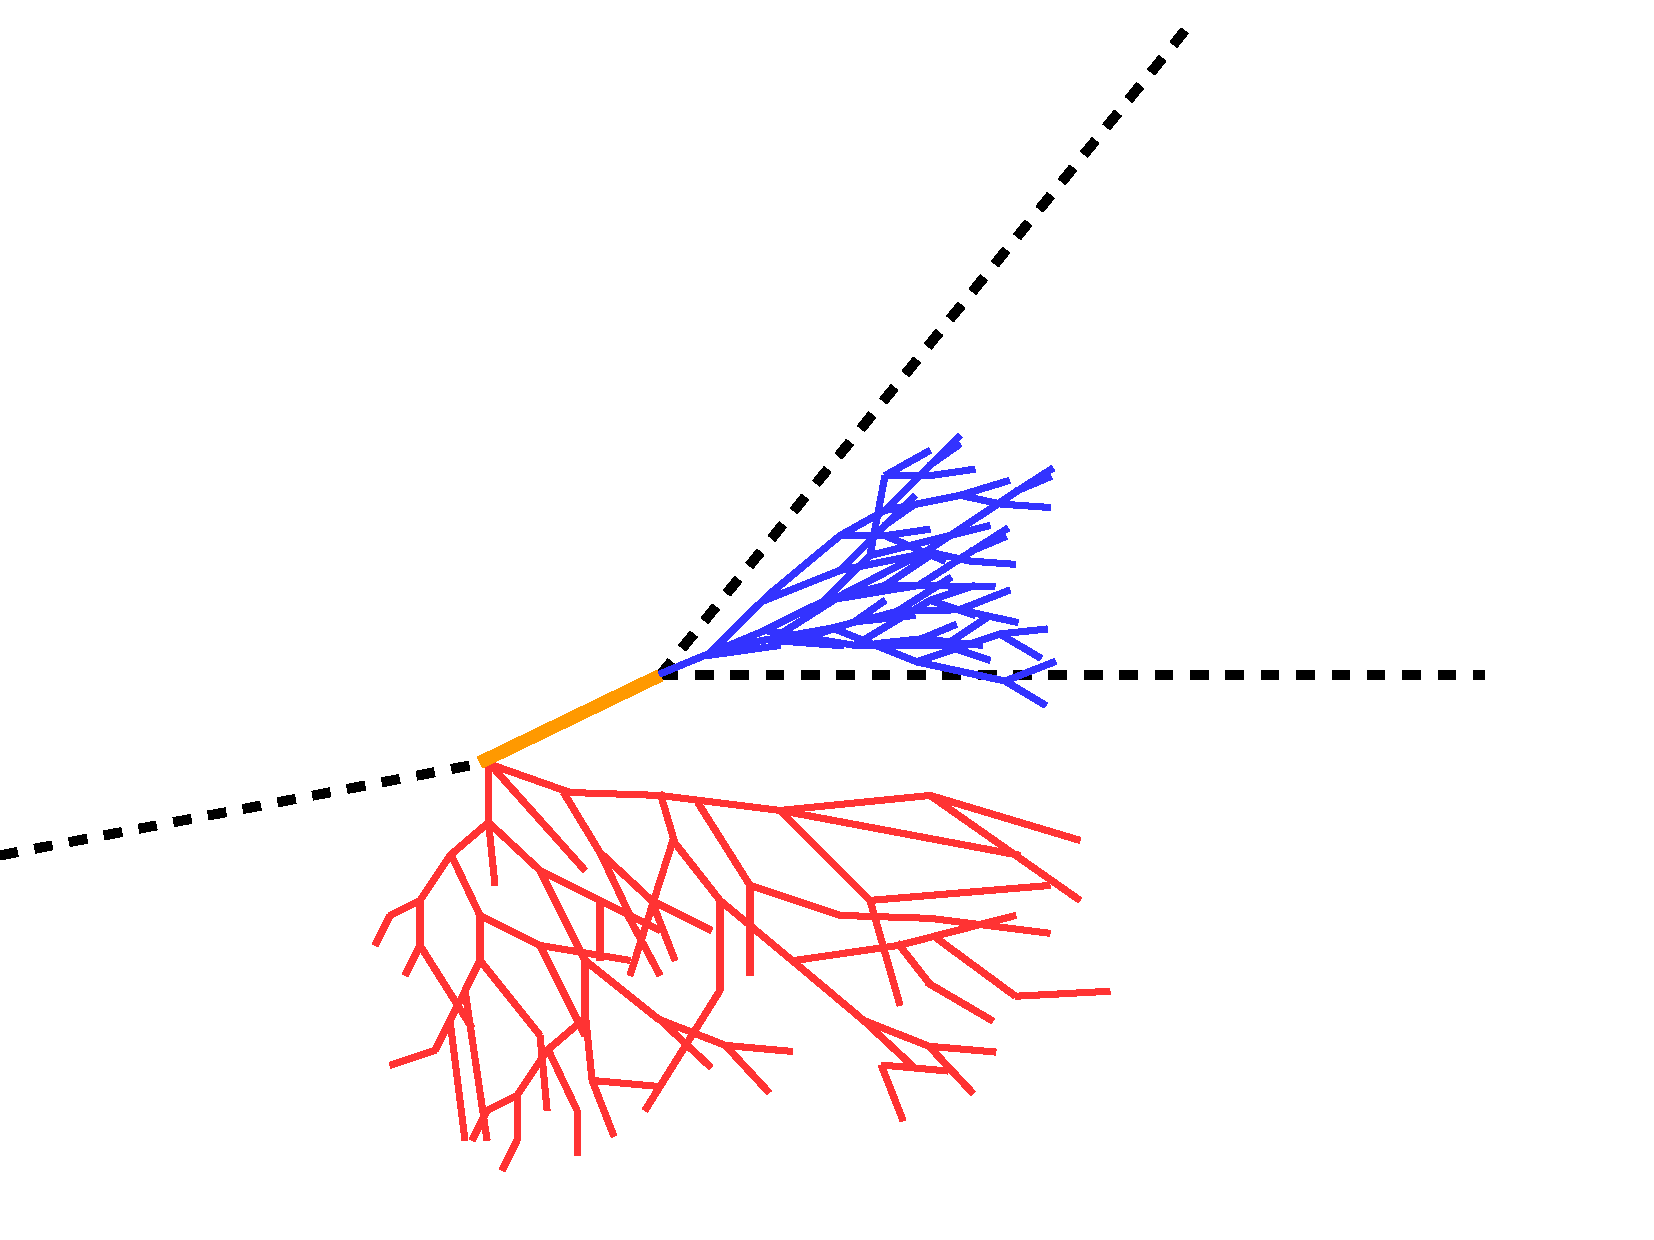
\includegraphics[width=2cm]{figures/neutrinos_properties/interaction_schematics/nutau_CC_cascadeonly.pdf}
            & $\tau^\pm$ decaying into $e^\pm$ or hadrons ($\sim$83\% BR)  
            & \\

            \cmidrule{1-3} CC $\overset{(-)}{\nu_e}$ 
            & 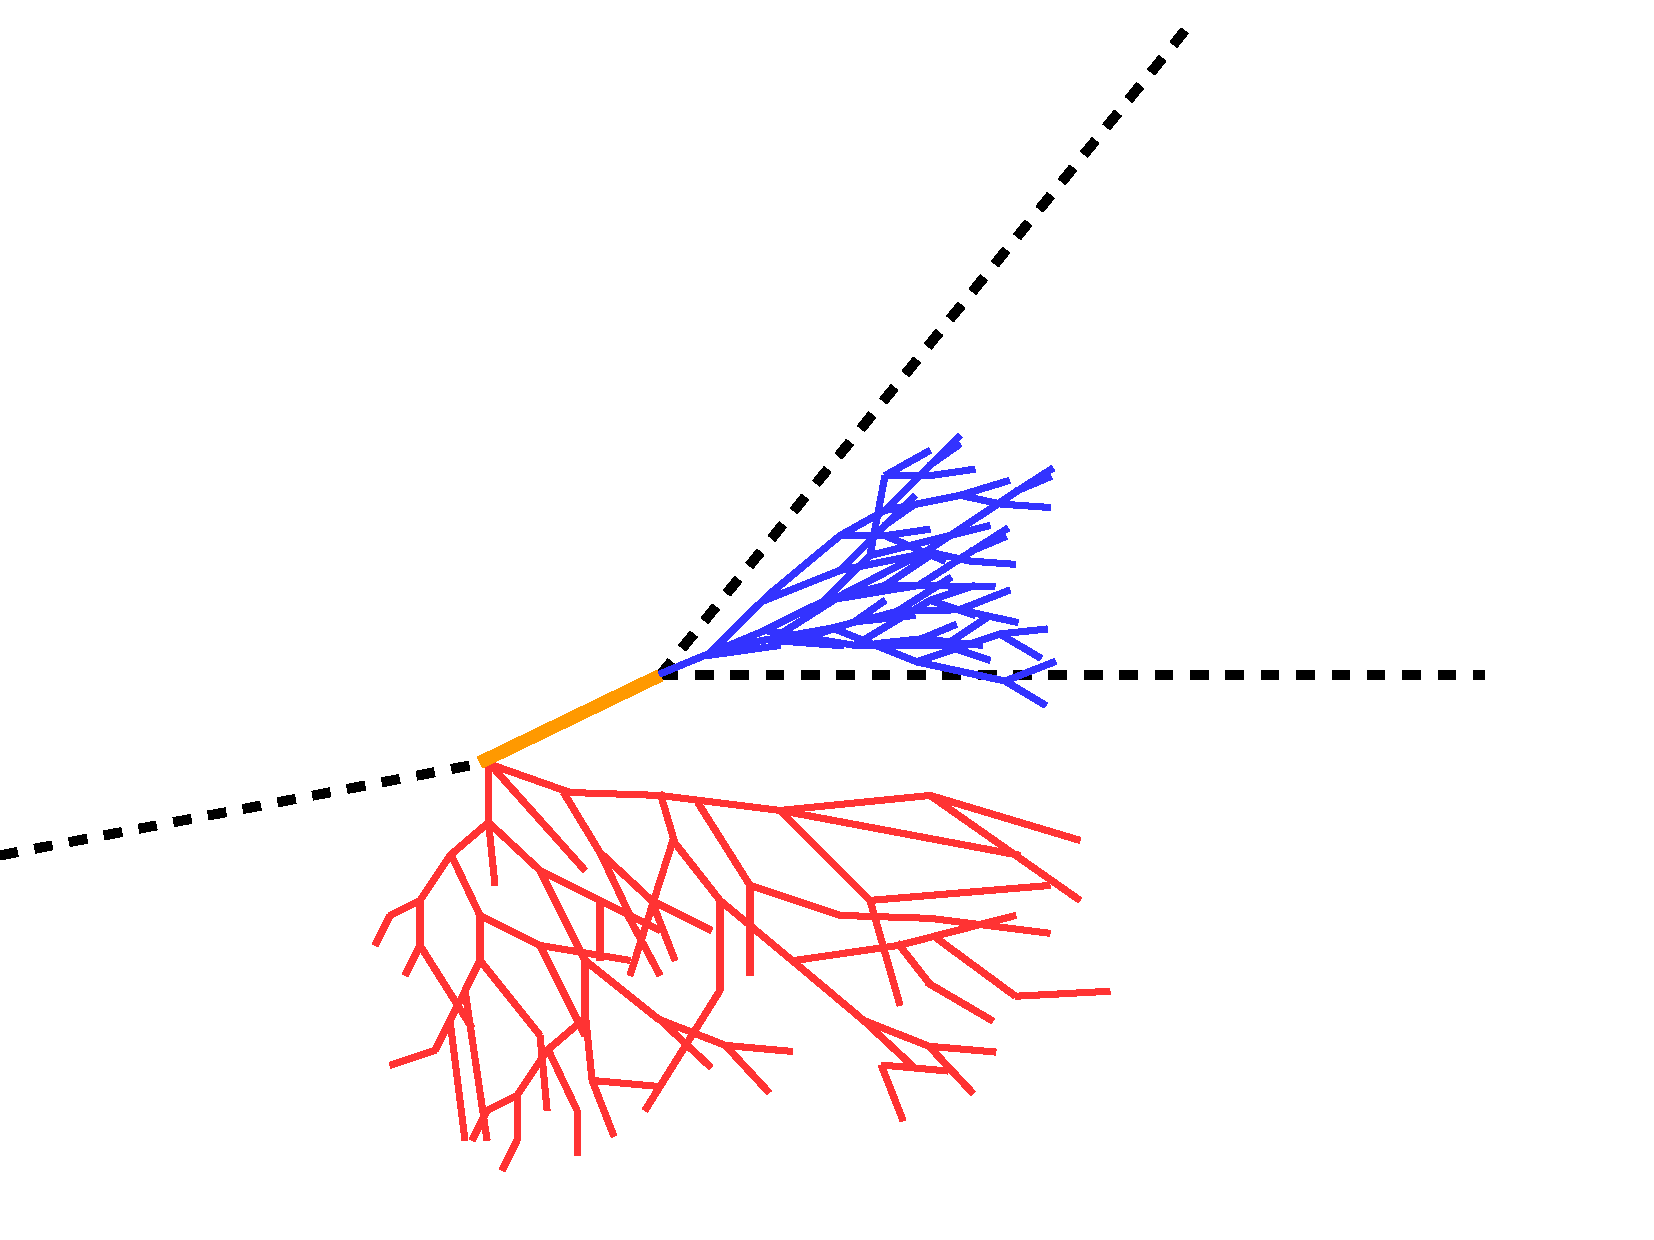
\includegraphics[width=2cm]{figures/neutrinos_properties/interaction_schematics/nue_CC_cascadeonly.pdf}
            & $e^\pm$, hadrons & {Cascade-only} \\

            \cmidrule{1-3}

            NC $\overset{(-)}{\nu_\ell}$ 
            & 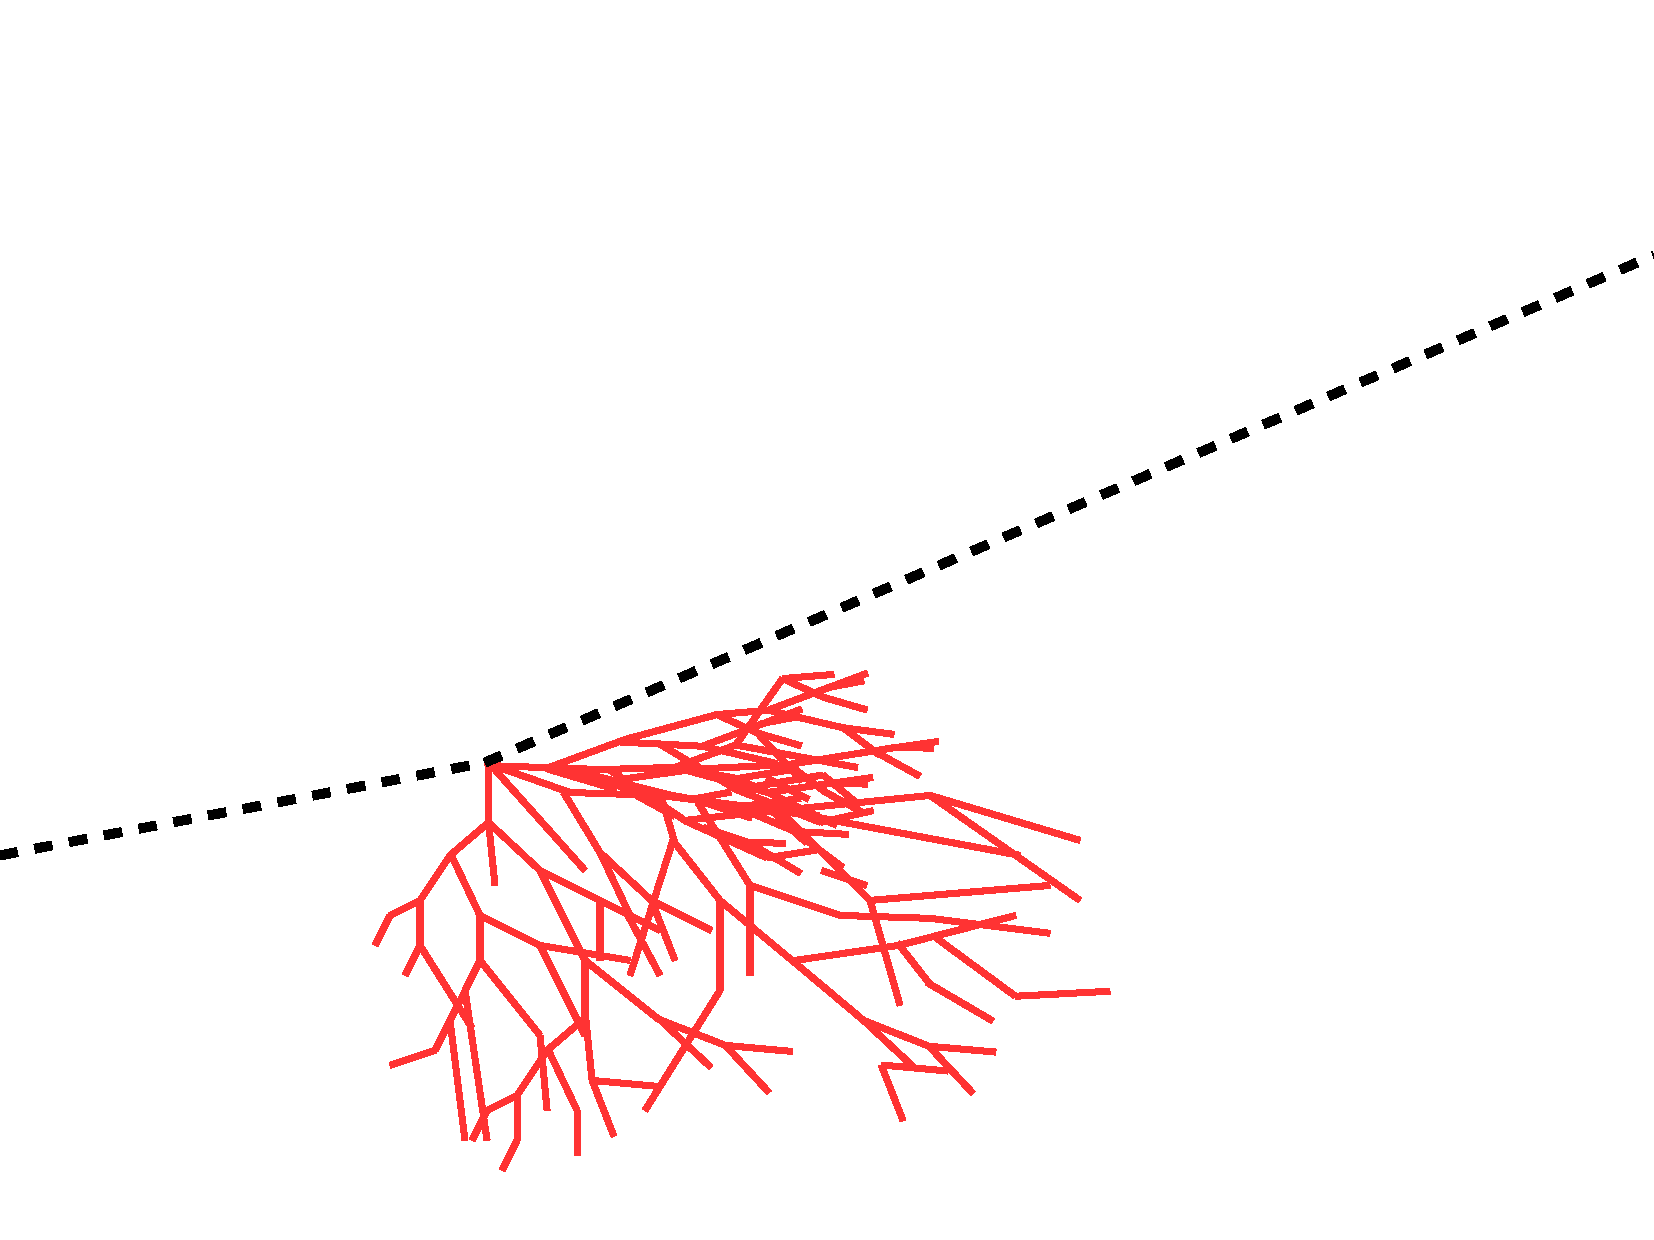
\includegraphics[width=2cm]{figures/neutrinos_properties/interaction_schematics/nuall_NC_cascadeonly.pdf} 
            & hadrons & \\

            \hline
        \end{tabular}
    \end{center}
    \caption[IceCube low energy event signatures and underlying interactions]{IceCube low energy event signatures, their underlying interaction type, and the particles that produce them. Also shown are the secondary particles produced in the interactions. Black dashed lines represent neutrinos, green lines muons, orange line leptons, and blue and red lines are particles in electromagnetic and hadronic cascades, respectively. Adapted from \cite{ATerliuk}.}
    \labtab{interactions_vs_signatures}
\end{table}


\paragraph{Neutrino} interactions are observed as cascades, tracks, or a combination of both, depending on the initial flavor and the interaction type for the specific event.

In $\nu_\mu$ - CC interactions, a muon is produced in addition to a hadronic shower from the breaking nucleus. If the interaction happens outside the detector, but the muon passes through the detector, this will create a track-like signature. The same happens if the interaction happens inside, but the energy transfer to the nucleus is small ($y \approx 0$). At energies relevant for this work, tracks have length at the same order of the distance between DOMs, so they can be observed as such.

If the interaction happens inside the detector and the energy transfer to the hadronic part of the shower is larger, it will create a cascade with a track leaving it. A similar signature is observed after a $\nu_\tau$ - CC interaction, in which a tau is produced that later decays into a muon, with a branching ratio of $\SI{17}{\percent}$.
% occurs if a $\nu_\tau$ - CC interaction happens, creating a tau that decays into a muon (happening with a branching ratio of $\SI{17}{\percent}$).
In those cases the muon usually has a lower energy and the track will be fainter and harder to observe.

The other $\SI{83}{\percent}$ of $\nu_\tau$ - CC interactions produce a tau that decays into an electron or hadrons, leaving a cascade-only signature through the electromagnetic or hadronic shower. All $\nu_e$ - CC interactions also produce pure cascades, since the electron quickly loses its energy in an electromagnetic shower. In all $\nu$ - NC interactions, the produced neutrino escapes and only the hadronic shower is observable. Since the size of the cascades at the energy range of interest is smaller than the spacing of the DOMs, they are approximately observed as point-like, spherical light sources. Even though the light is almost isotropically emitted, some assymmetry remains in the light profile, which can be used to reconstruct the direction of the incoming neutrino.


\paragraph{Atmospheric muons} also produce pure track like signatures, similar to $\nu_\mu$ - CC interactions happening outside the detector. They are one of the main backgrounds for analyses using atmospheric neutrinos and are therefore the target of many filter steps described in \refsec{trigger_and_filter}.


% \setchapterstyle{kao}
\setchapterpreamble[u]{\margintoc}

\chapter{Heavy Neutral Lepton Signal Simulation}
\labch{signal_simulation}

After the SM simulation generation and the default low energy event selection and processing chain were introduced in the previous \refch{simulation_and_processing}, the focus will now be on the central part of this thesis - the HNL signal simulation. Since this is the first attempt of performing a search for HNLs with IceCube DeepCore, there was no prior knowledge of the expected performance nor the event expectation and the simulation had to be developed from scratch. Two avenues of simulation generation were pursued in parallel; a collection of model independent simulation sets was realized and is explained in \refsec{model_independent_simulation} and the physically accurate model dependent simulation is described in \refsec{model_specific_simulation}.


\section{Model Independent Simulation} \labsec{model_independent_simulation}

To investigate the potential of IceCube to detect HNLs by identifying the unique double cascade morphology explained in \refsec{double_cascade_morphology}, it is very valuable to have simulation sets where the double cascade kinematics can be controlled directly. In a realistic model the decay kinematics and the absolute event expectation all depend on the specific model parameters chosen (see \refsec{hnl_theory}). To decouple the simulation from a specific model, a model independent double cascade generator was developed and will be explained in the following sections. Using these sets, the performance of IceCube DeepCore to detect low energetic double cascades, dependent on their properties, is studied in \refch{double_cascade_performance}.


\subsection{Generator Functions}




\textbf{Implemented generator functions:}
\begin{itemize}
    \item random sign 
    \item power law sampling
    \item exponential sampling
    \item[] 
    \item direction vector (from zenith/azimuth)
    \item direction angles (from direction vector)
    \item[] 
    \item make cascade (produce EM cascade particle from pos, dir, energy, time)
    \item add cascades to tree (add n cascades to mctree)
\end{itemize}


\todo{Re-write/re-formulate this section (copied from HNL technote).}

For this purpose a collection of secondary generator functions is added to the \href{https://github.com/LeanderFischer/LeptonInjector-HNL/blob/main/LeptonInjector/python/cascade_generator_functions.py}{custom LeptonInjector project}. It includes a function to place an arbitrary list of electromagnetic cascades (electrons) with given positions, directions, and energies into an \textit{I3MCTree} and add it to the current frame. There is also some functions used to create the individual cascades and for specific random sampling. Note here that the icetray random number generators should always be used in order to avoid issues with the tray scope and multiple files having identical distributions. To simulate a specific set a process script needs to be set up that deals with sampling from the wanted distributions and calls the full generation in a tray script. For cluster submission using dagman, a submit and a job script are also needed. Explicit examples will be linked in the following sections, where specific choices for model independent simulation sets will be explained in more detail.

\subsection{Simplistic Sets}


\subsubsection{Up-Going/String 81 Centered Set}


\begin{figure}
    \centering
    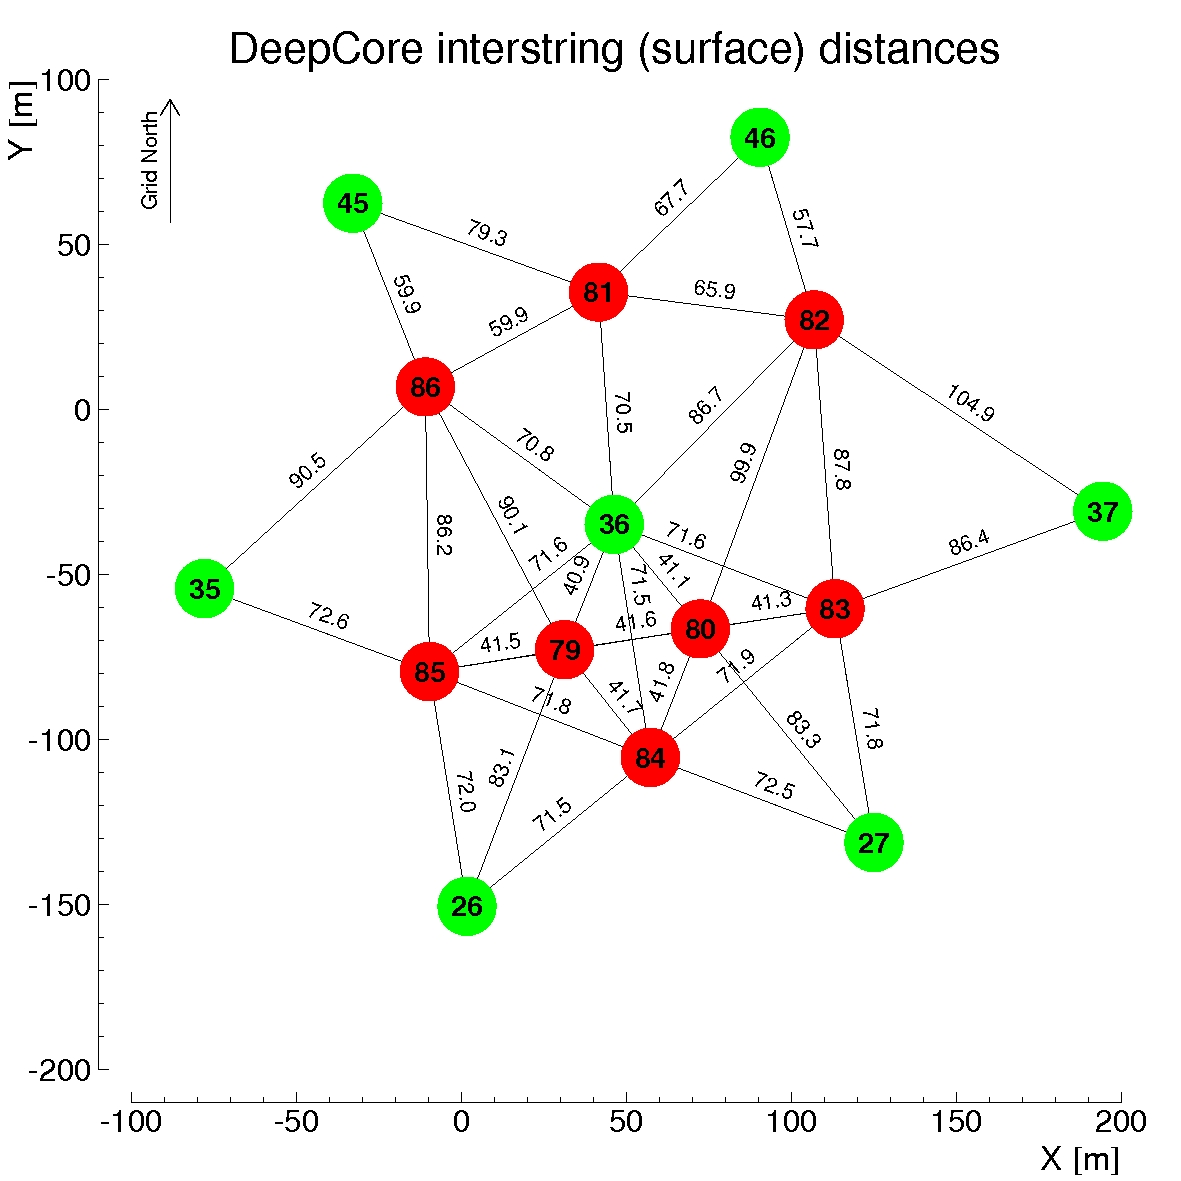
\includegraphics{figures/icecube_deepcore/deepcore_surface_distances.jpg}
    \caption[xx]{Horizontal positions and distances between DeepCore strings. Red strings are instrumented more densely (vertically) and partially with higher quantum efficiency (HQE) DOMs.}
    \labfig{deepcore_distances}
\end{figure}

To investigate one of the best possible cases of detecting double cascades, a set is produced, where both cascades are placed on a DeepCore string (namely string 81) and the directions are directly up-going. The horizontal positions of all DeepCore strings are shown in \reffig{deepcore_distances}. The z position of each cascade is sampled uniformly along the strings z elongation and the energies are sampled uniform in [$0.0, 60.0$]\si{\gev}. The order of the cascades is chosen such that the lower one is first ($t_0=0.0$) and the upper one is second ($t_1=L/c$). The sampling distributions/values for the cascades are listed in \reftab{upgoing_string81_sampling_distributions}. The generation level distributions of the sampled variables are shown in \reffig{upgoing_string81_gen_distris}.


\begin{table*}
        \begin{tabular}{ llll }
        \hline\hline
        \textbf{Set} & \textbf{Variable} & \textbf{Distribution} & \textbf{Range/Value} \\
        \hline\hline
        Up-going &&& \\
        \hline
        & energy & uniform & [0.0, 60.0]\si{\gev} \\
        & zenith & fixed & \SI{180.0}{\degree} \\
        & azimuth & fixed & \SI{0.0}{\degree} \\
        & ($x,y$) position & fixed & (41.6, 35.49)\si{\metre} \\
        & $z$ position & uniform & [-480.0, -180.0]\si{\metre} \\
        \hline
        Horizontal &&& \\ 
        \hline
        & energy & uniform & [0.0, 60.0]\si{\gev} \\
        & zenith & fixed & \SI{90.0}{\degree} \\
        & azimuth & uniform & [0.0, 360.0]\si{\degree} \\
        & ($x,y$) position & uniform (circle) & $c$=(46.29, -34.88)\si{\metre}, $r$=\SI{150.0}{\metre} \\
        & $z$ position & fixed & \SI{-330.0}{\metre} \\
        \hline
        \end{tabular}
    \caption[xx]{Sampling distributions of up-going, string 81 centered and horizontal simulation generation.}
    \labtab{hnl_simplified_set_sampling_distributions}
\end{table*}


% \begin{figure}[h!]
%     \subfloat[\labfig{upgoing_string81_gen_distris_energies}]{
%         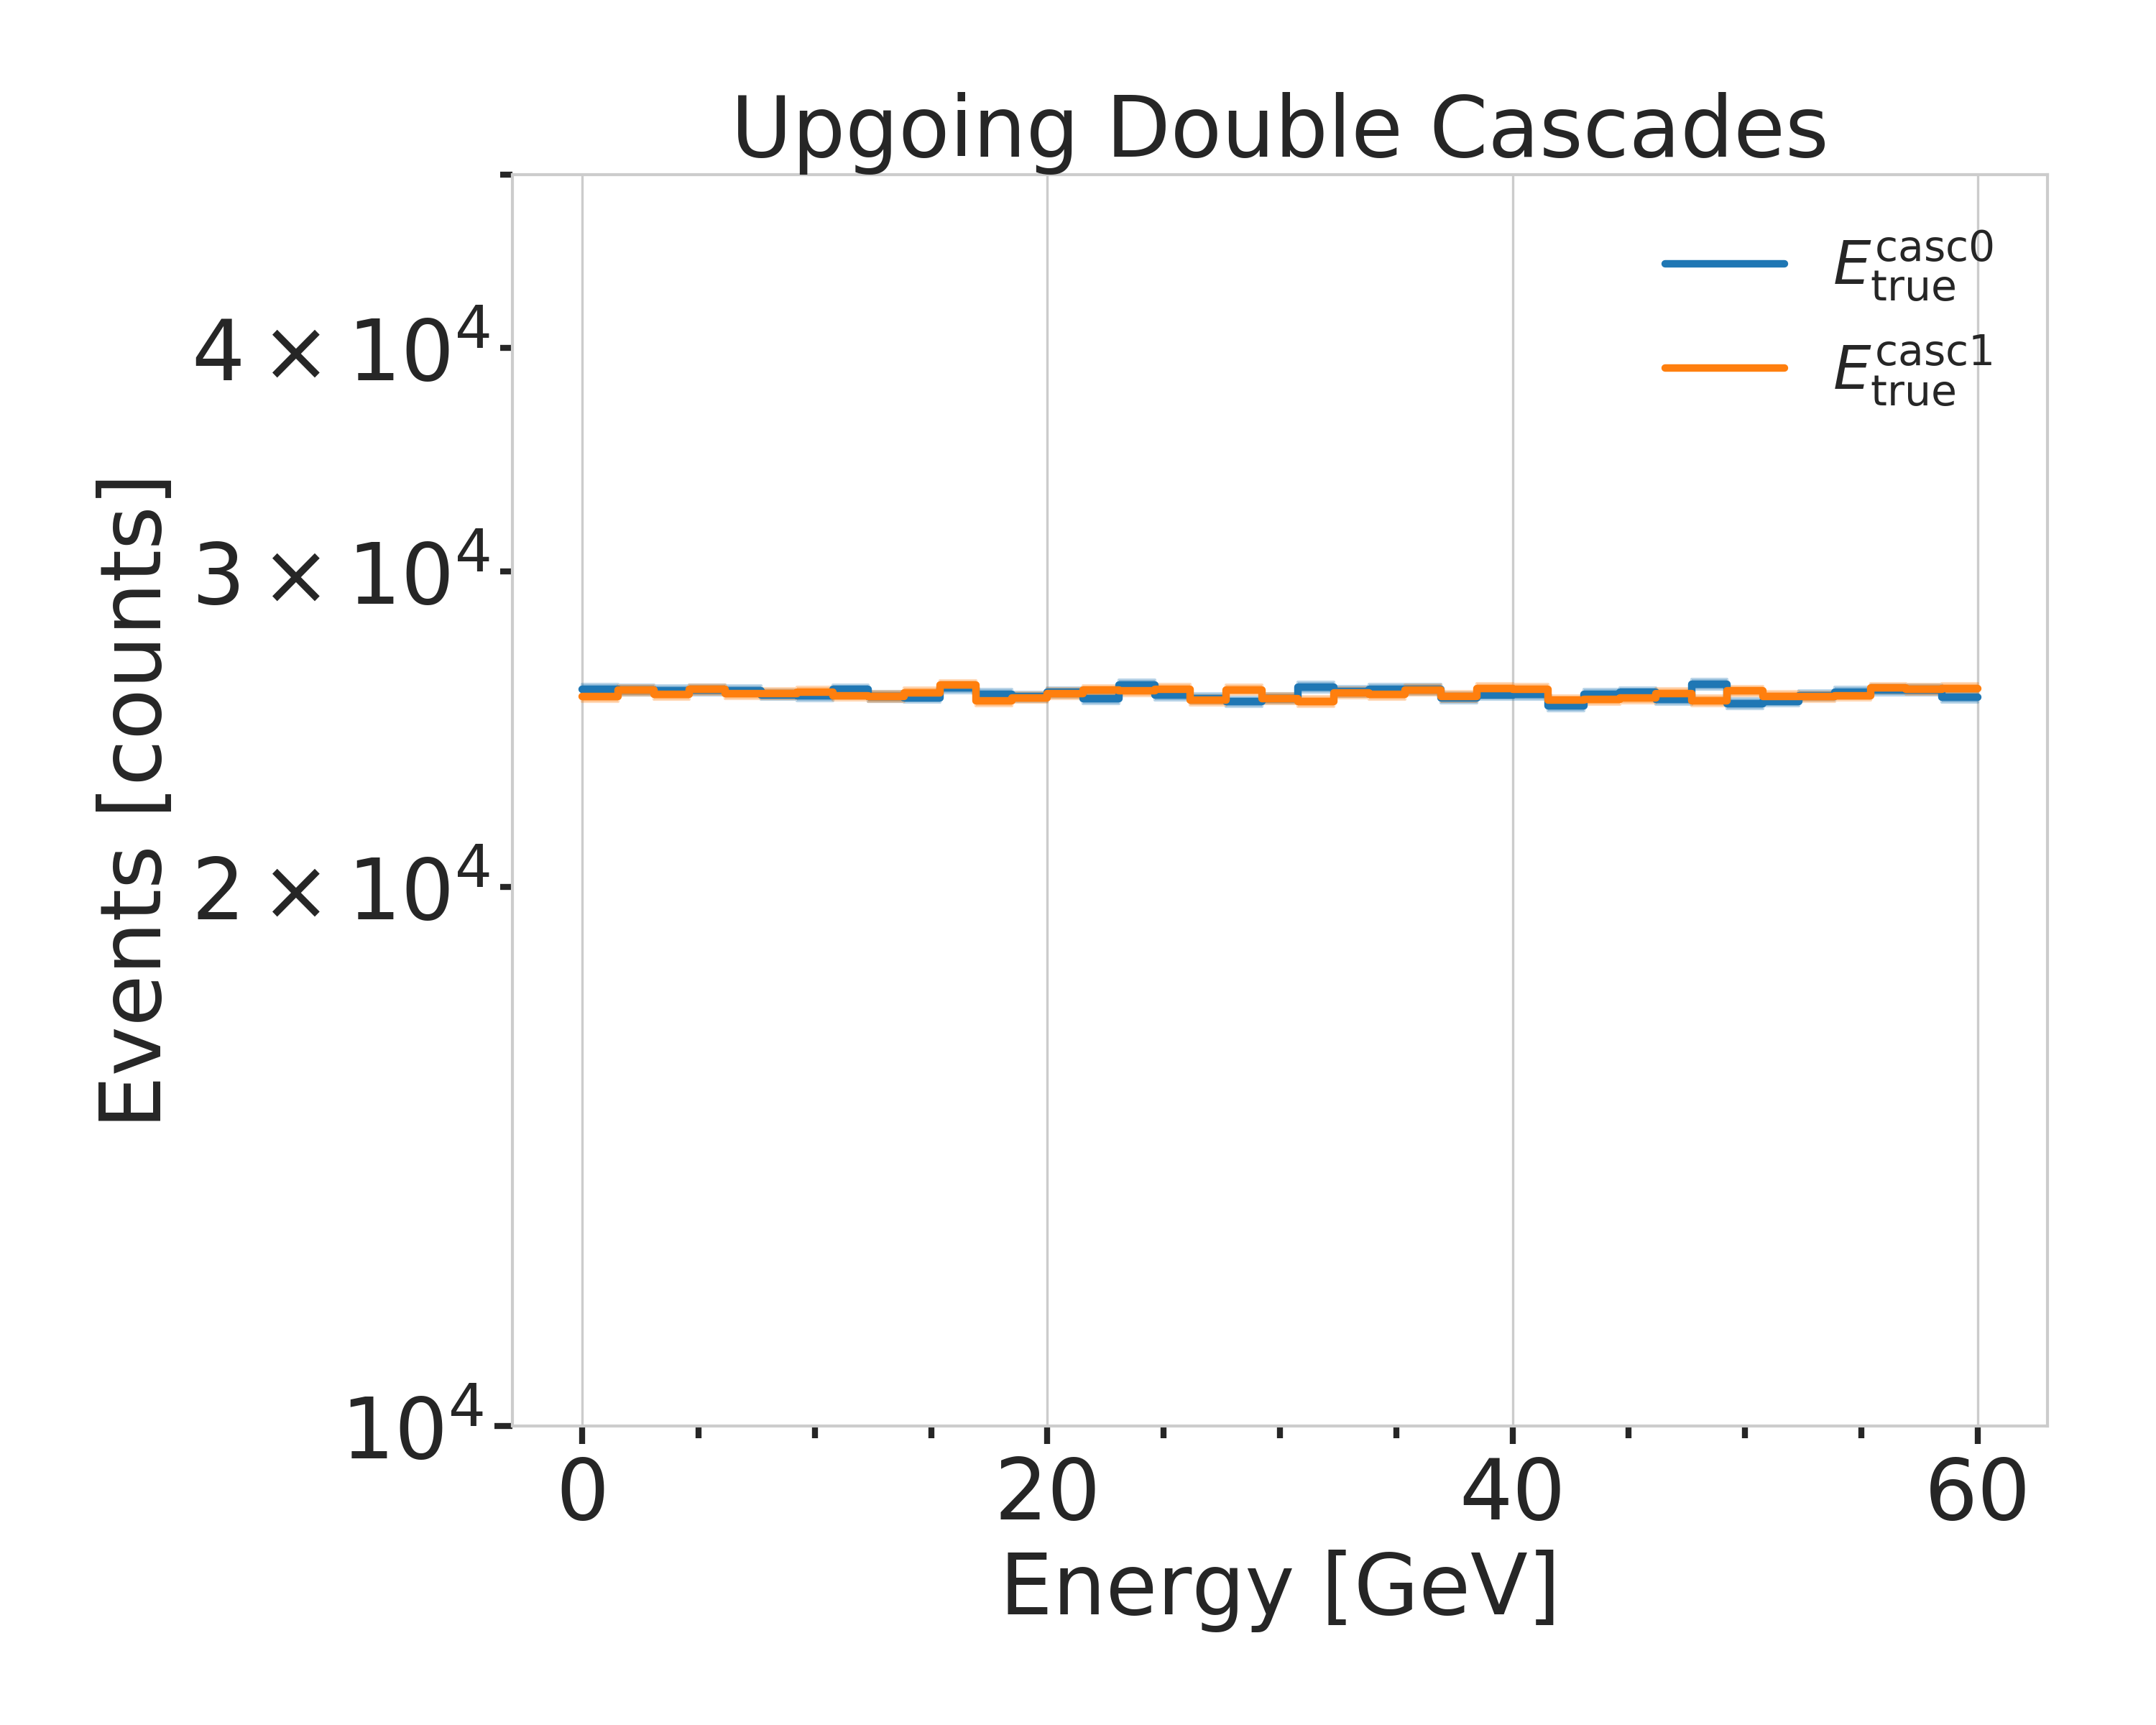
\includegraphics[width=.45\linewidth]{figures/upgoing_string_81_gen_level/1_d_distr_energies_clipped.png}
%     }
%     \subfloat[\labfig{upgoing_string81_gen_distris_depths}]{
%         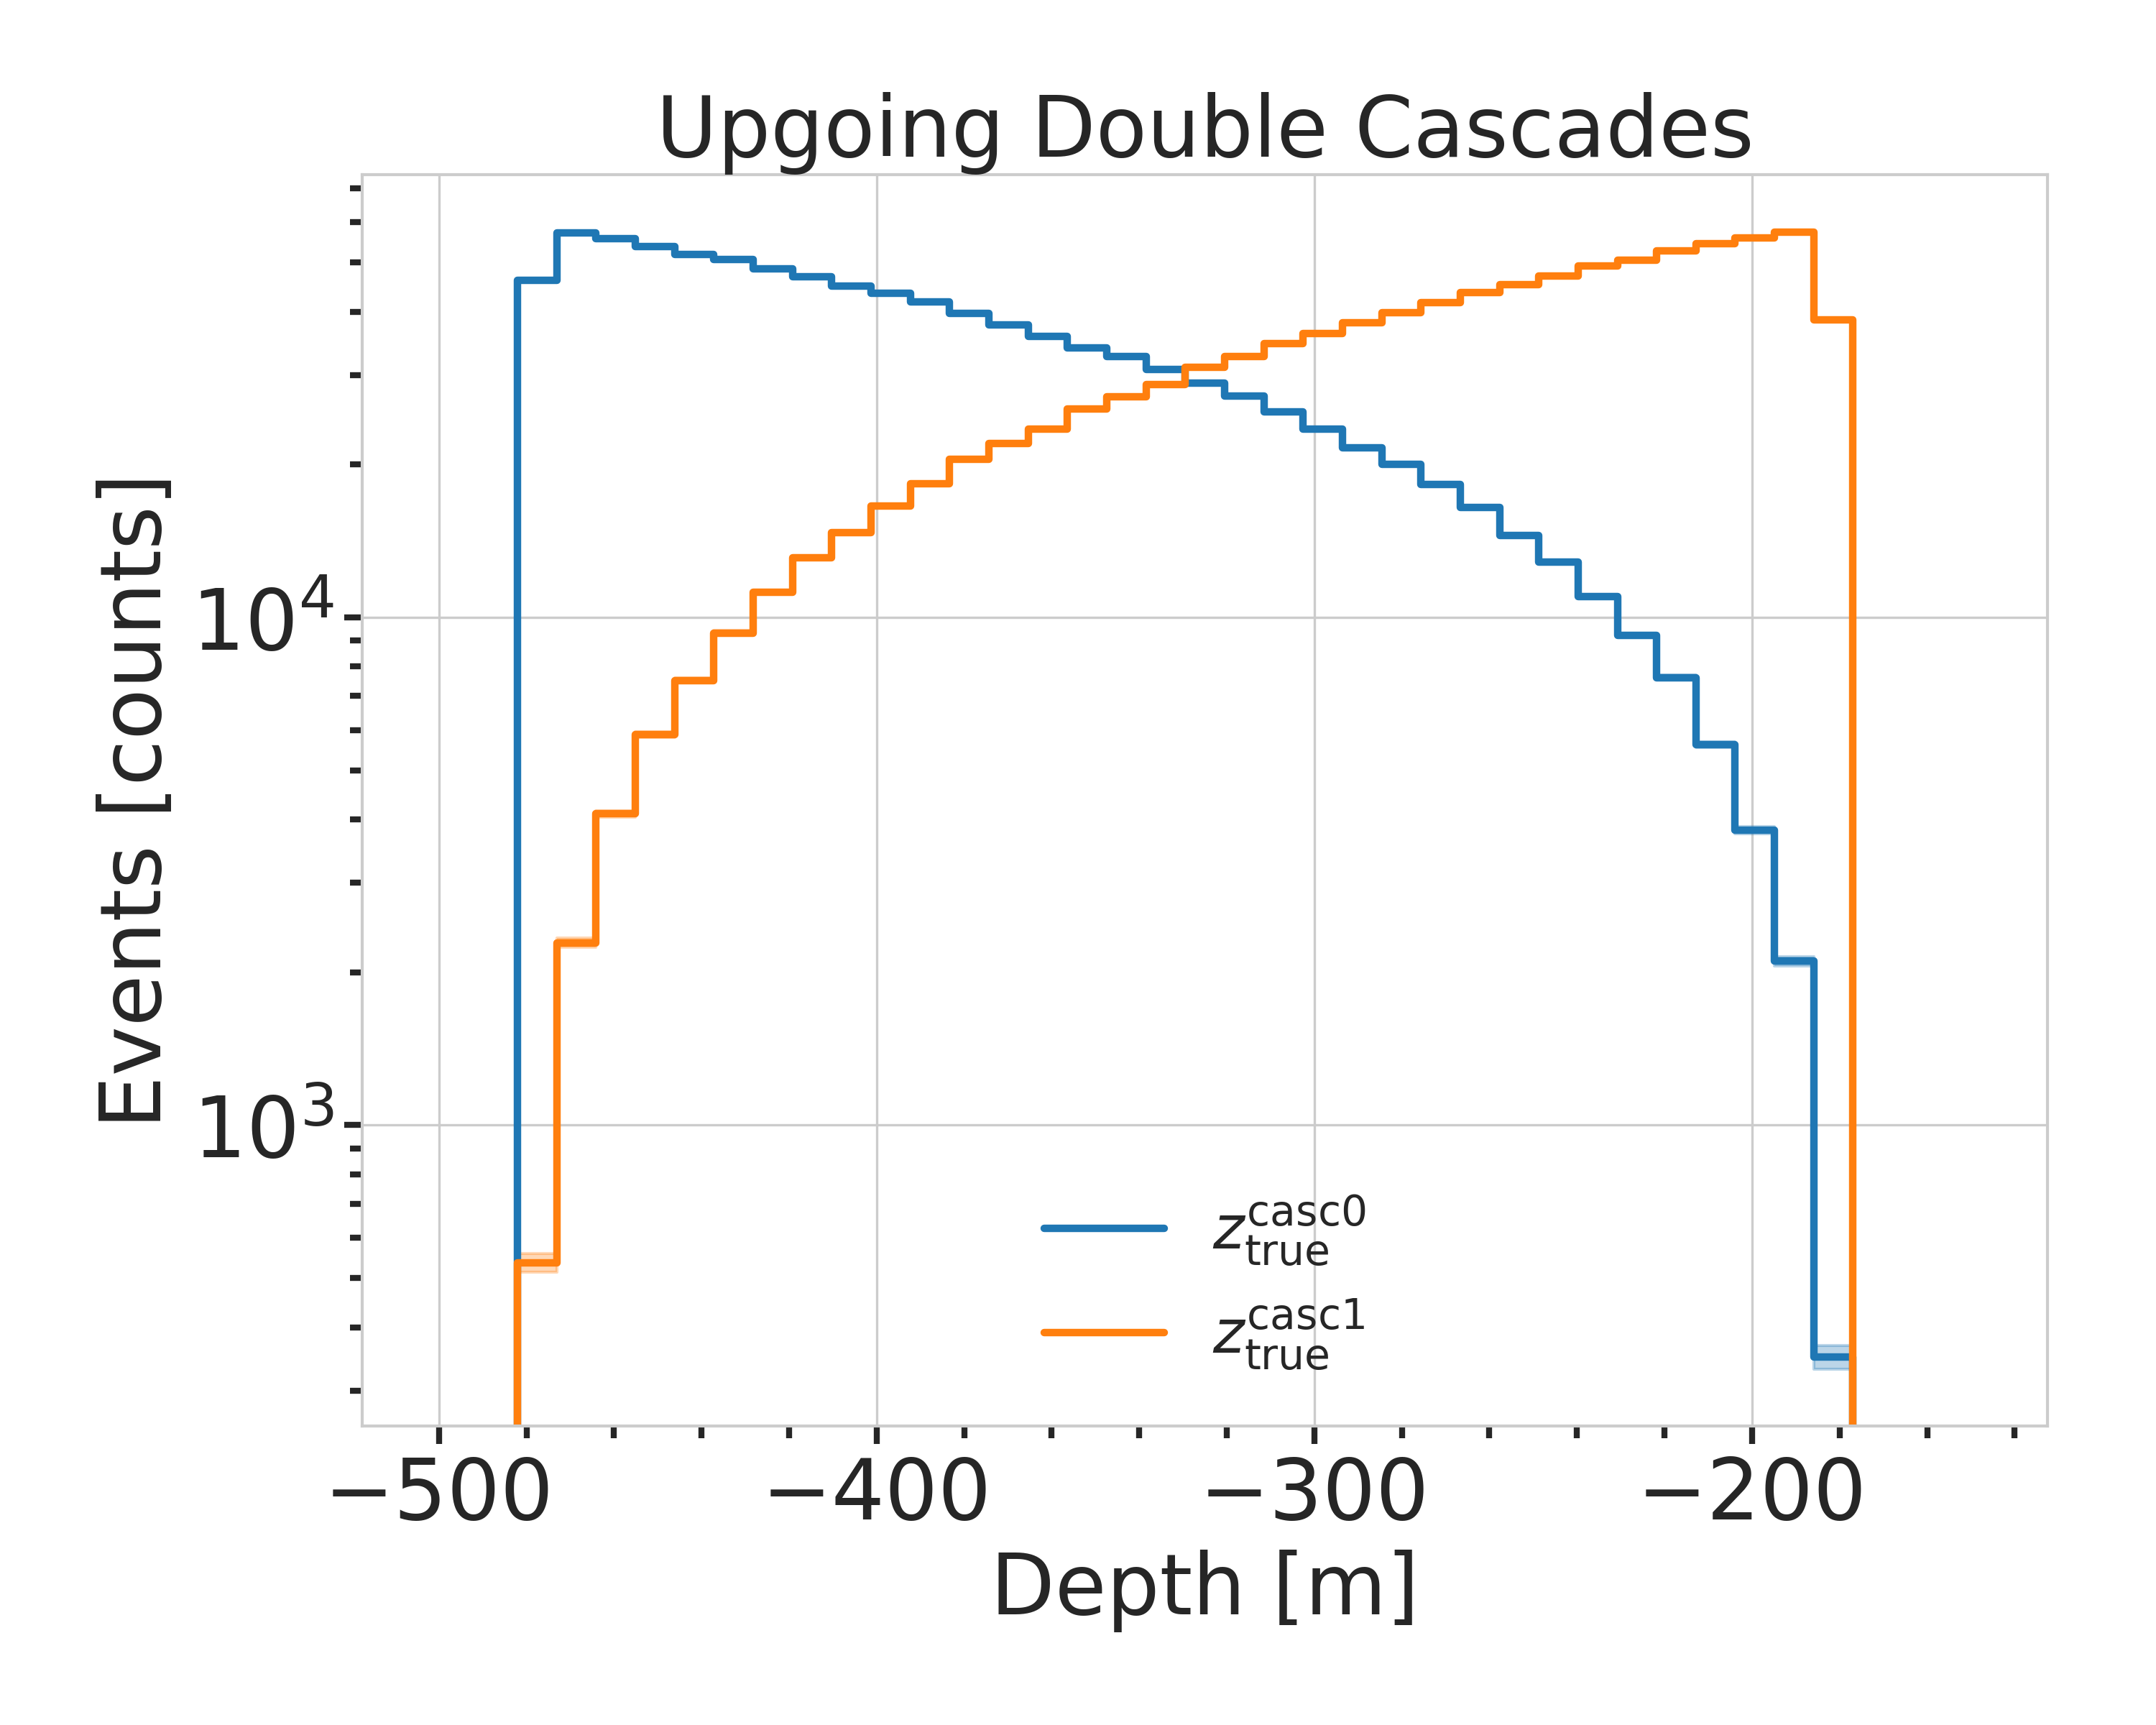
\includegraphics[width=.45\linewidth]{figures/upgoing_string_81_gen_level/1_d_distr_depths_clipped.png}
%     }
%     \\[-2.5ex]
%     \subfloat[\labfig{upgoing_string81_gen_distris_decay_length}]{
%         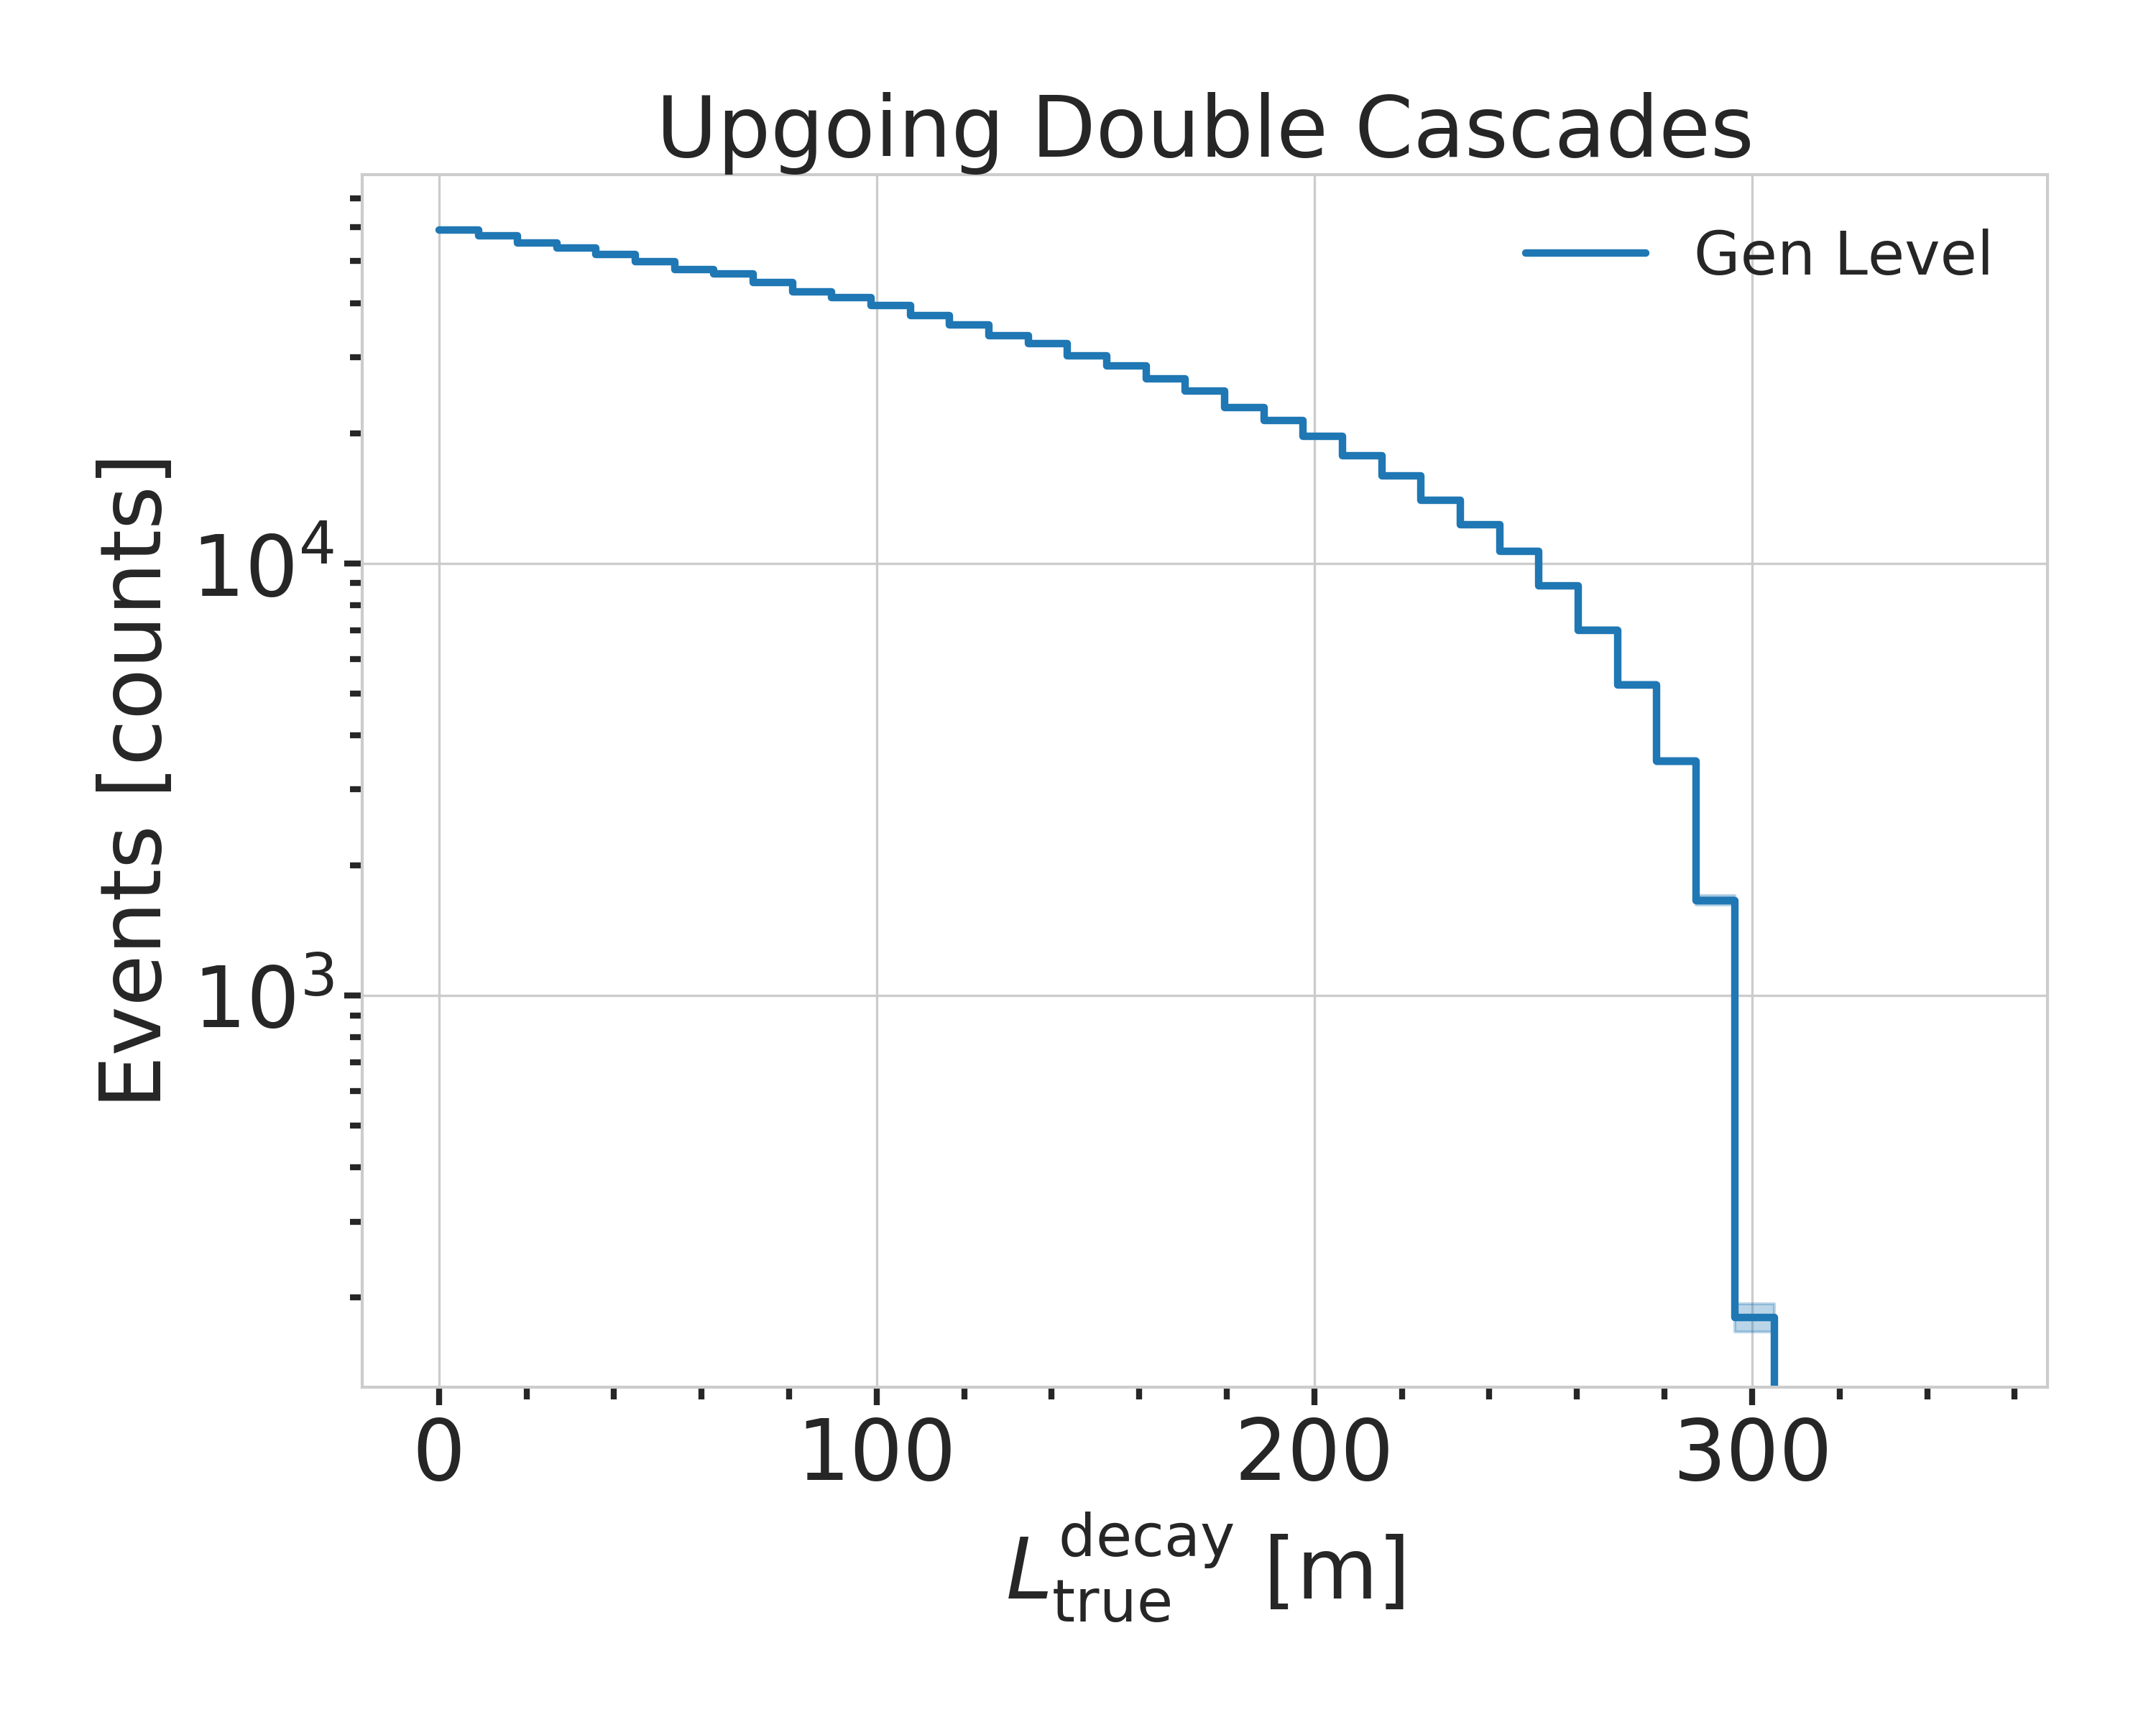
\includegraphics[width=.45\linewidth]{figures/upgoing_string_81_gen_level/1_d_distr_true_decay_length_clipped.png}
%     }
%     \subfloat[\labfig{upgoing_string81_gen_distris_total_energy}]{
%         \includegraphics[width=.45\linewidth]{figures/upgoing_string_81_gen_level/1_d_distr_true_total_energy_clipped.png}
%     }
%     \caption{Generation level distributions of the 1000 files, with 1000 events each of set 194601. Only the parameters that are not fixed to a certain value are shown.}
%     \labfig{upgoing_string81_gen_distris}
% \end{figure}

After generation the events are processed with standard Photon, Detector, L1, and L2 processing and then Taupede+MuMillipede is run on top of the L2 files. Multiple versions with different parameters were produced, some with the OscNext baseline parameters, some without detector noise (in Det level) and some with h2-50cm holeice model, to match the holeice model that was used to generate the photonics tables.


\paragraph{BrightDom Cleaning}

To investigate the effect of the BrightDom cleaning cut the 194601 set without detector noise (and baseline hole ice model) is used. The BrightDom cleaning is needed to stop a few DOMs with many photon hits to drive the reconstruction because this leads to large biases in the energy estimations. Historically, the BrightDom cleaning was removing all DOMs that had a charge larger than 10 times the mean charge. After quickly checking some charge distributions and how the mean behaves it was clear that the cut should better be defined based on a metric that is less affected by outliers, like the median. \reffig{bright_dom_cleaning_charges_mean_median} shows where the mean and the median are located for an example event. The cut was re-defined to use the median instead of the mean and 10\% of the simulation were processed with \href{https://github.com/LeanderFischer/I3_HNL_Decay/blob/a6838ec48e0a2d4f6547cbe064d2928ec55fb76d/submission_scripts/process/process_Taupede.py}{Taupede} using 30x and 100x the median as BrightDom cutoff. \reffig{bright_dom_cleaning_charges_median_scales} shows where these values fall for the same example event.

% \begin{figure}[h!]
%     \subfloat[\labfig{bright_dom_cleaning_charges_mean_median}]{
%         \includegraphics[width=.45\linewidth]{figures/upgoing_string_81_gen_level/brightdom_cleaning/median_and_mean_L2_00001.i3.zst_SplitInIcePulses_frame_0.png}
%         }
%     \subfloat[\labfig{bright_dom_cleaning_charges_median_scales}]{
%         \includegraphics[width=.45\linewidth]{figures/upgoing_string_81_gen_level/brightdom_cleaning/median_scales_L2_00001.i3.zst_SplitInIcePulses_frame_0.png}
%         }
%     \caption{Charge distribution of example event showing mean and median charge (left) and different scales of median charge (right).}
%     \labfig{bright_dom_cleaning_charges}
% \end{figure}

As a quick check of the performance of both cuts the decay length resolution/bias and the resolutions/biases of all energies were checked. The reconstructed decay length is almost not affected by applying this cut, which is as expected, because it is mostly dependent on the arrival time of the photons. The effect on the reconstructed energy is much stronger, where a looser cut (100x) shows a significantly larger bias than the tighter cut at (30x). Even though this was not a highly sophisticated optimization of the BrightDom cut, an improvement was achieved by changing from mean to median and selecting the tighter cut (of the two tested). It's hard to tell how this would perform for high energy events, but I'm quite certain that a definition based on the median would be more reliable than on the mean.

% \begin{figure}[h!]
%     \subfloat[\labfig{bright_dom_cleaning_performance_decay_length_bias}]{
%         \includegraphics[width=.45\linewidth]{figures/upgoing_string_81_gen_level/brightdom_cleaning/median_decay_length_bias_fullset_larger_range_unweighted.png}
%         }
%     \subfloat[\labfig{bright_dom_cleaning_performance_total_energy_bias}]{
%         \includegraphics[width=.45\linewidth]{figures/upgoing_string_81_gen_level/brightdom_cleaning/compare_bright_dom_cuts_fractional_reco_total_energy_error_fully.png}
%         }
%     \caption{Decay length bias (left) and total energy bias (right).}
%     \labfig{bright_dom_cleaning_performance}
% \end{figure}


\subsubsection{Horizontal Set}

To investigate the effect of the tilt and the reconstruction performance for horizontal events another set is produced where both cascades are placed on a circle with radius $150$\si{\metre} at a depth of $-330$\si{\metre}. The direction is always horizontal (zenith=$\pi/2$) and azimuth is defined by the connecting vector of both random sampled cascade positions. The energies are again sampled uniform in [$0.0, 60.0$]\si{\gev}. The sampling distributions/values for the cascades are listed in \reftab{horizontal_sampling_distributions}. 

% The generation level distributions of the sampled variables are shown in \reffig{horizontal_gen_distris}.


% \begin{figure}[h!]
%     \subfloat[\labfig{horizontal_gen_distris_energies}]{
%         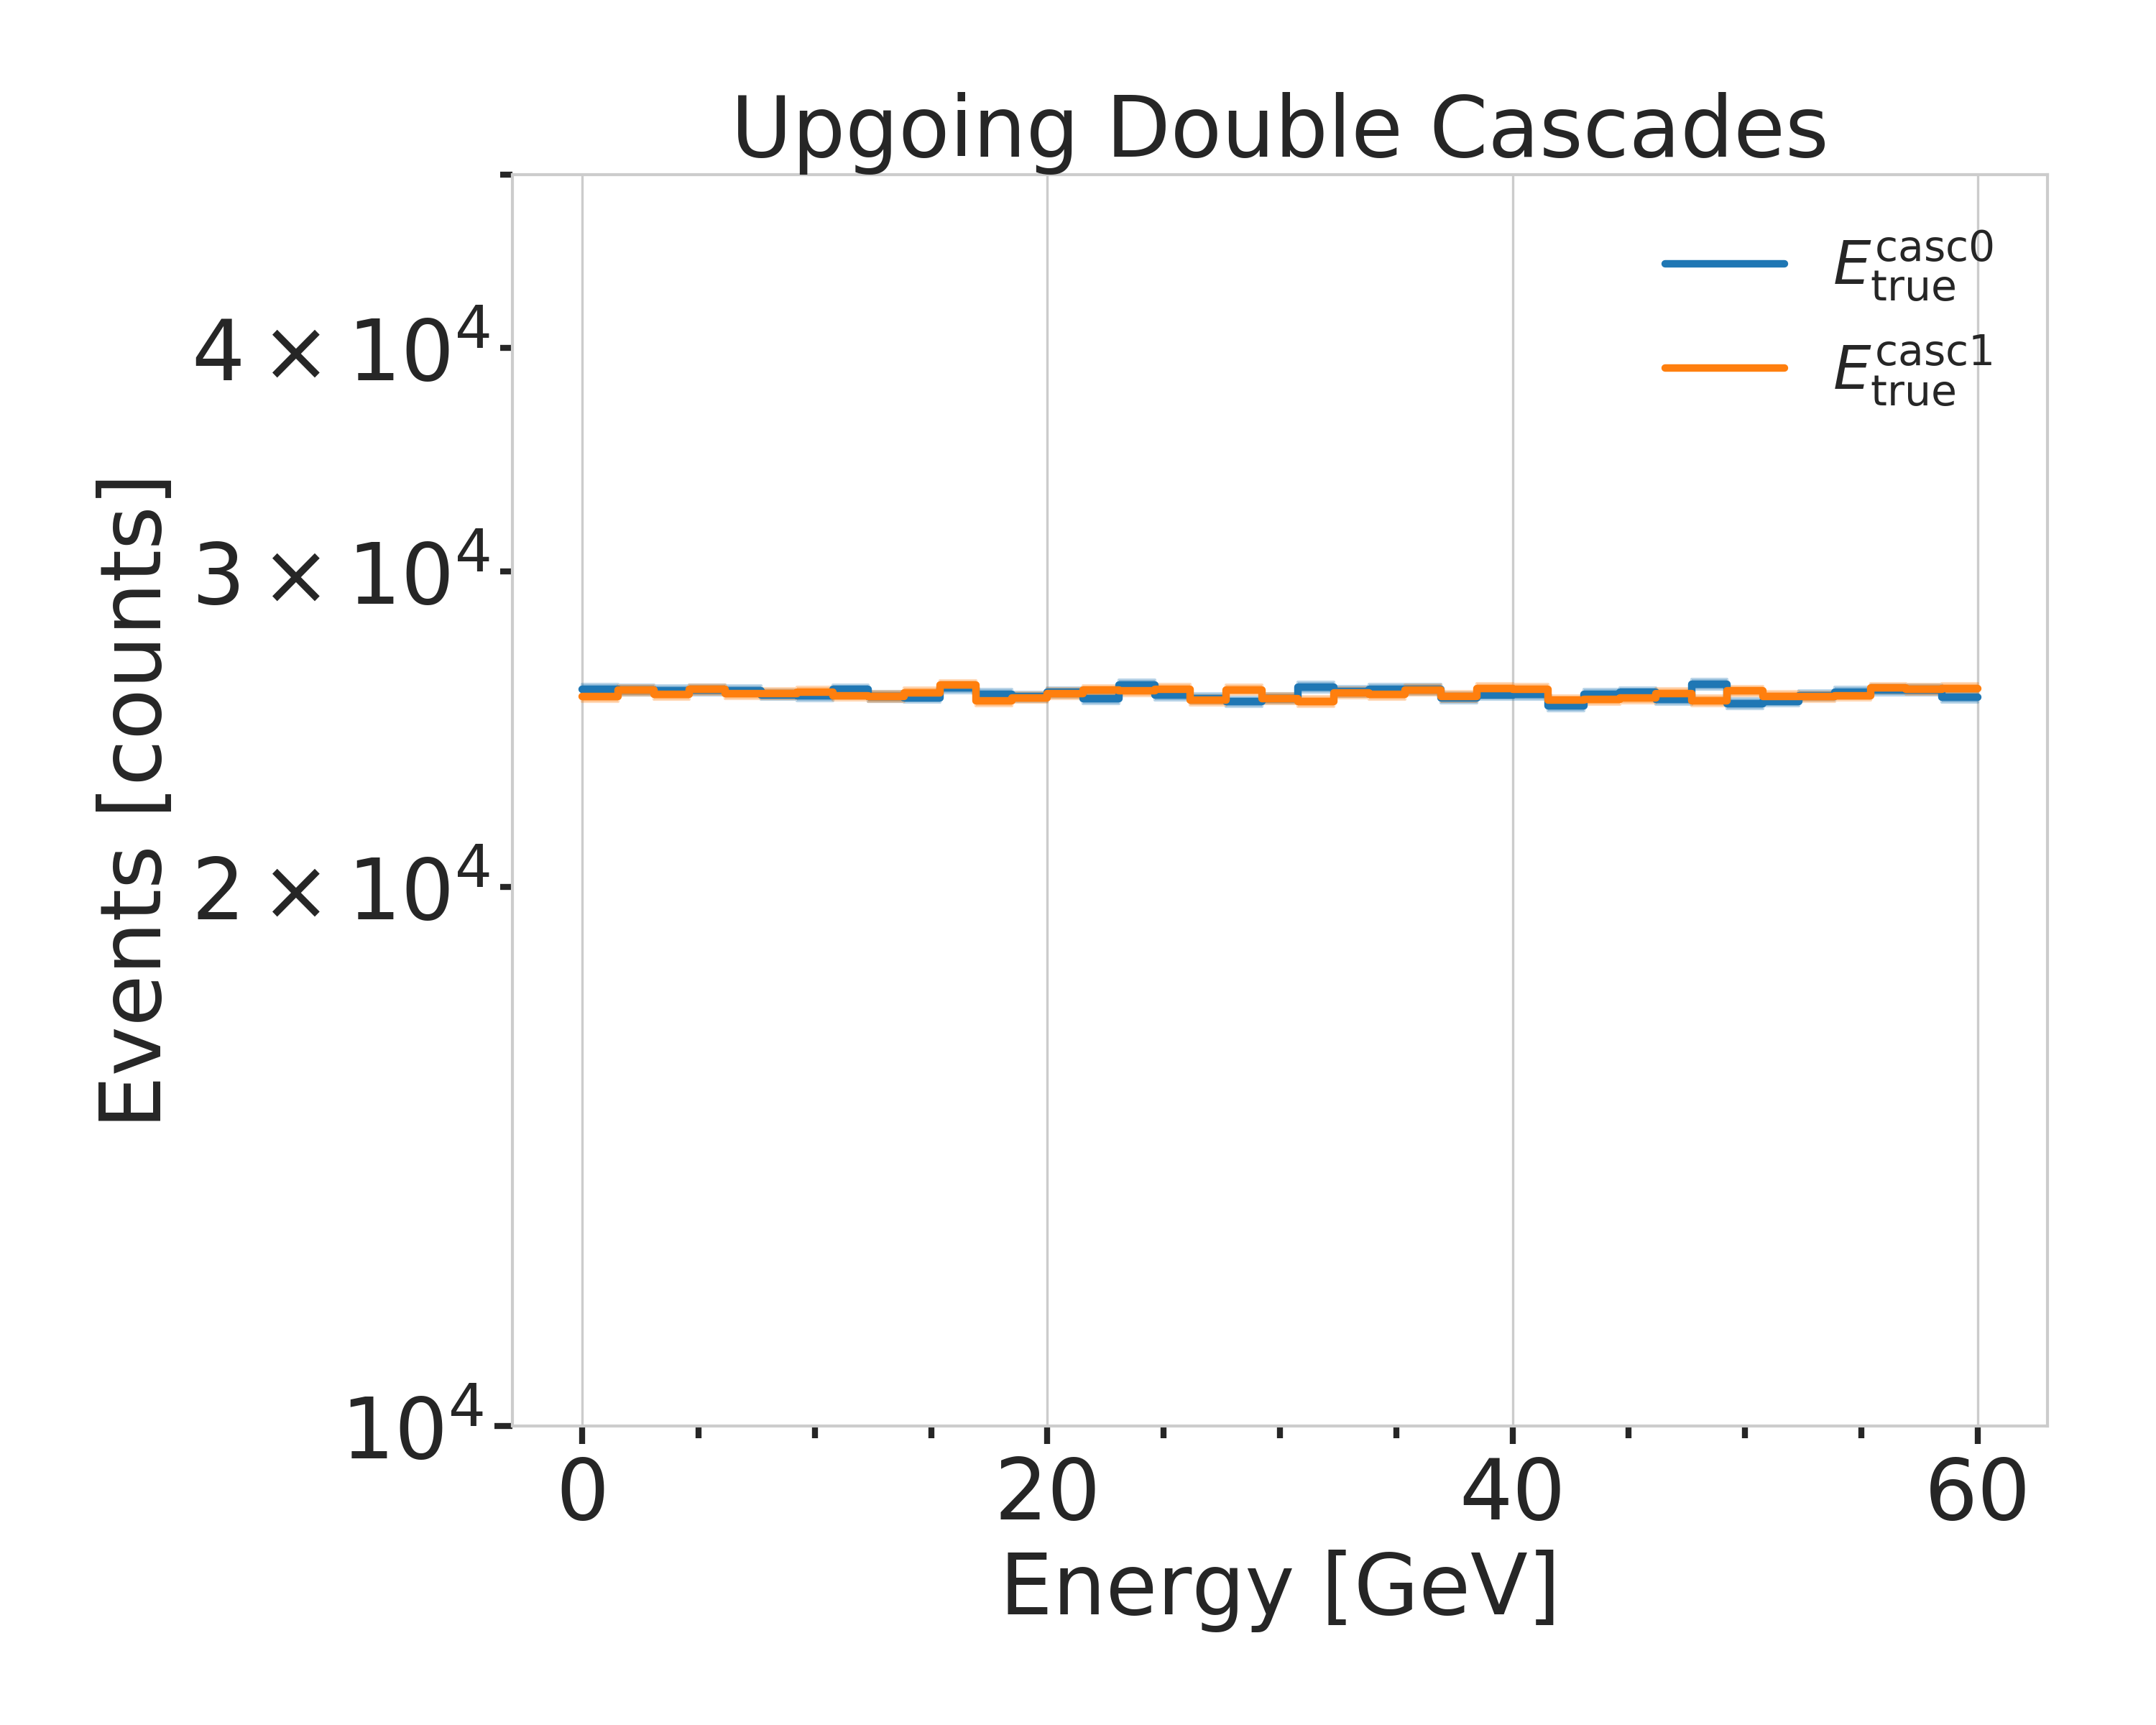
\includegraphics[width=.45\linewidth]{figures/upgoing_string_81_gen_level/1_d_distr_energies_clipped.png}
%     }
%     \subfloat[\labfig{horizontal_gen_distris_depths}]{
%         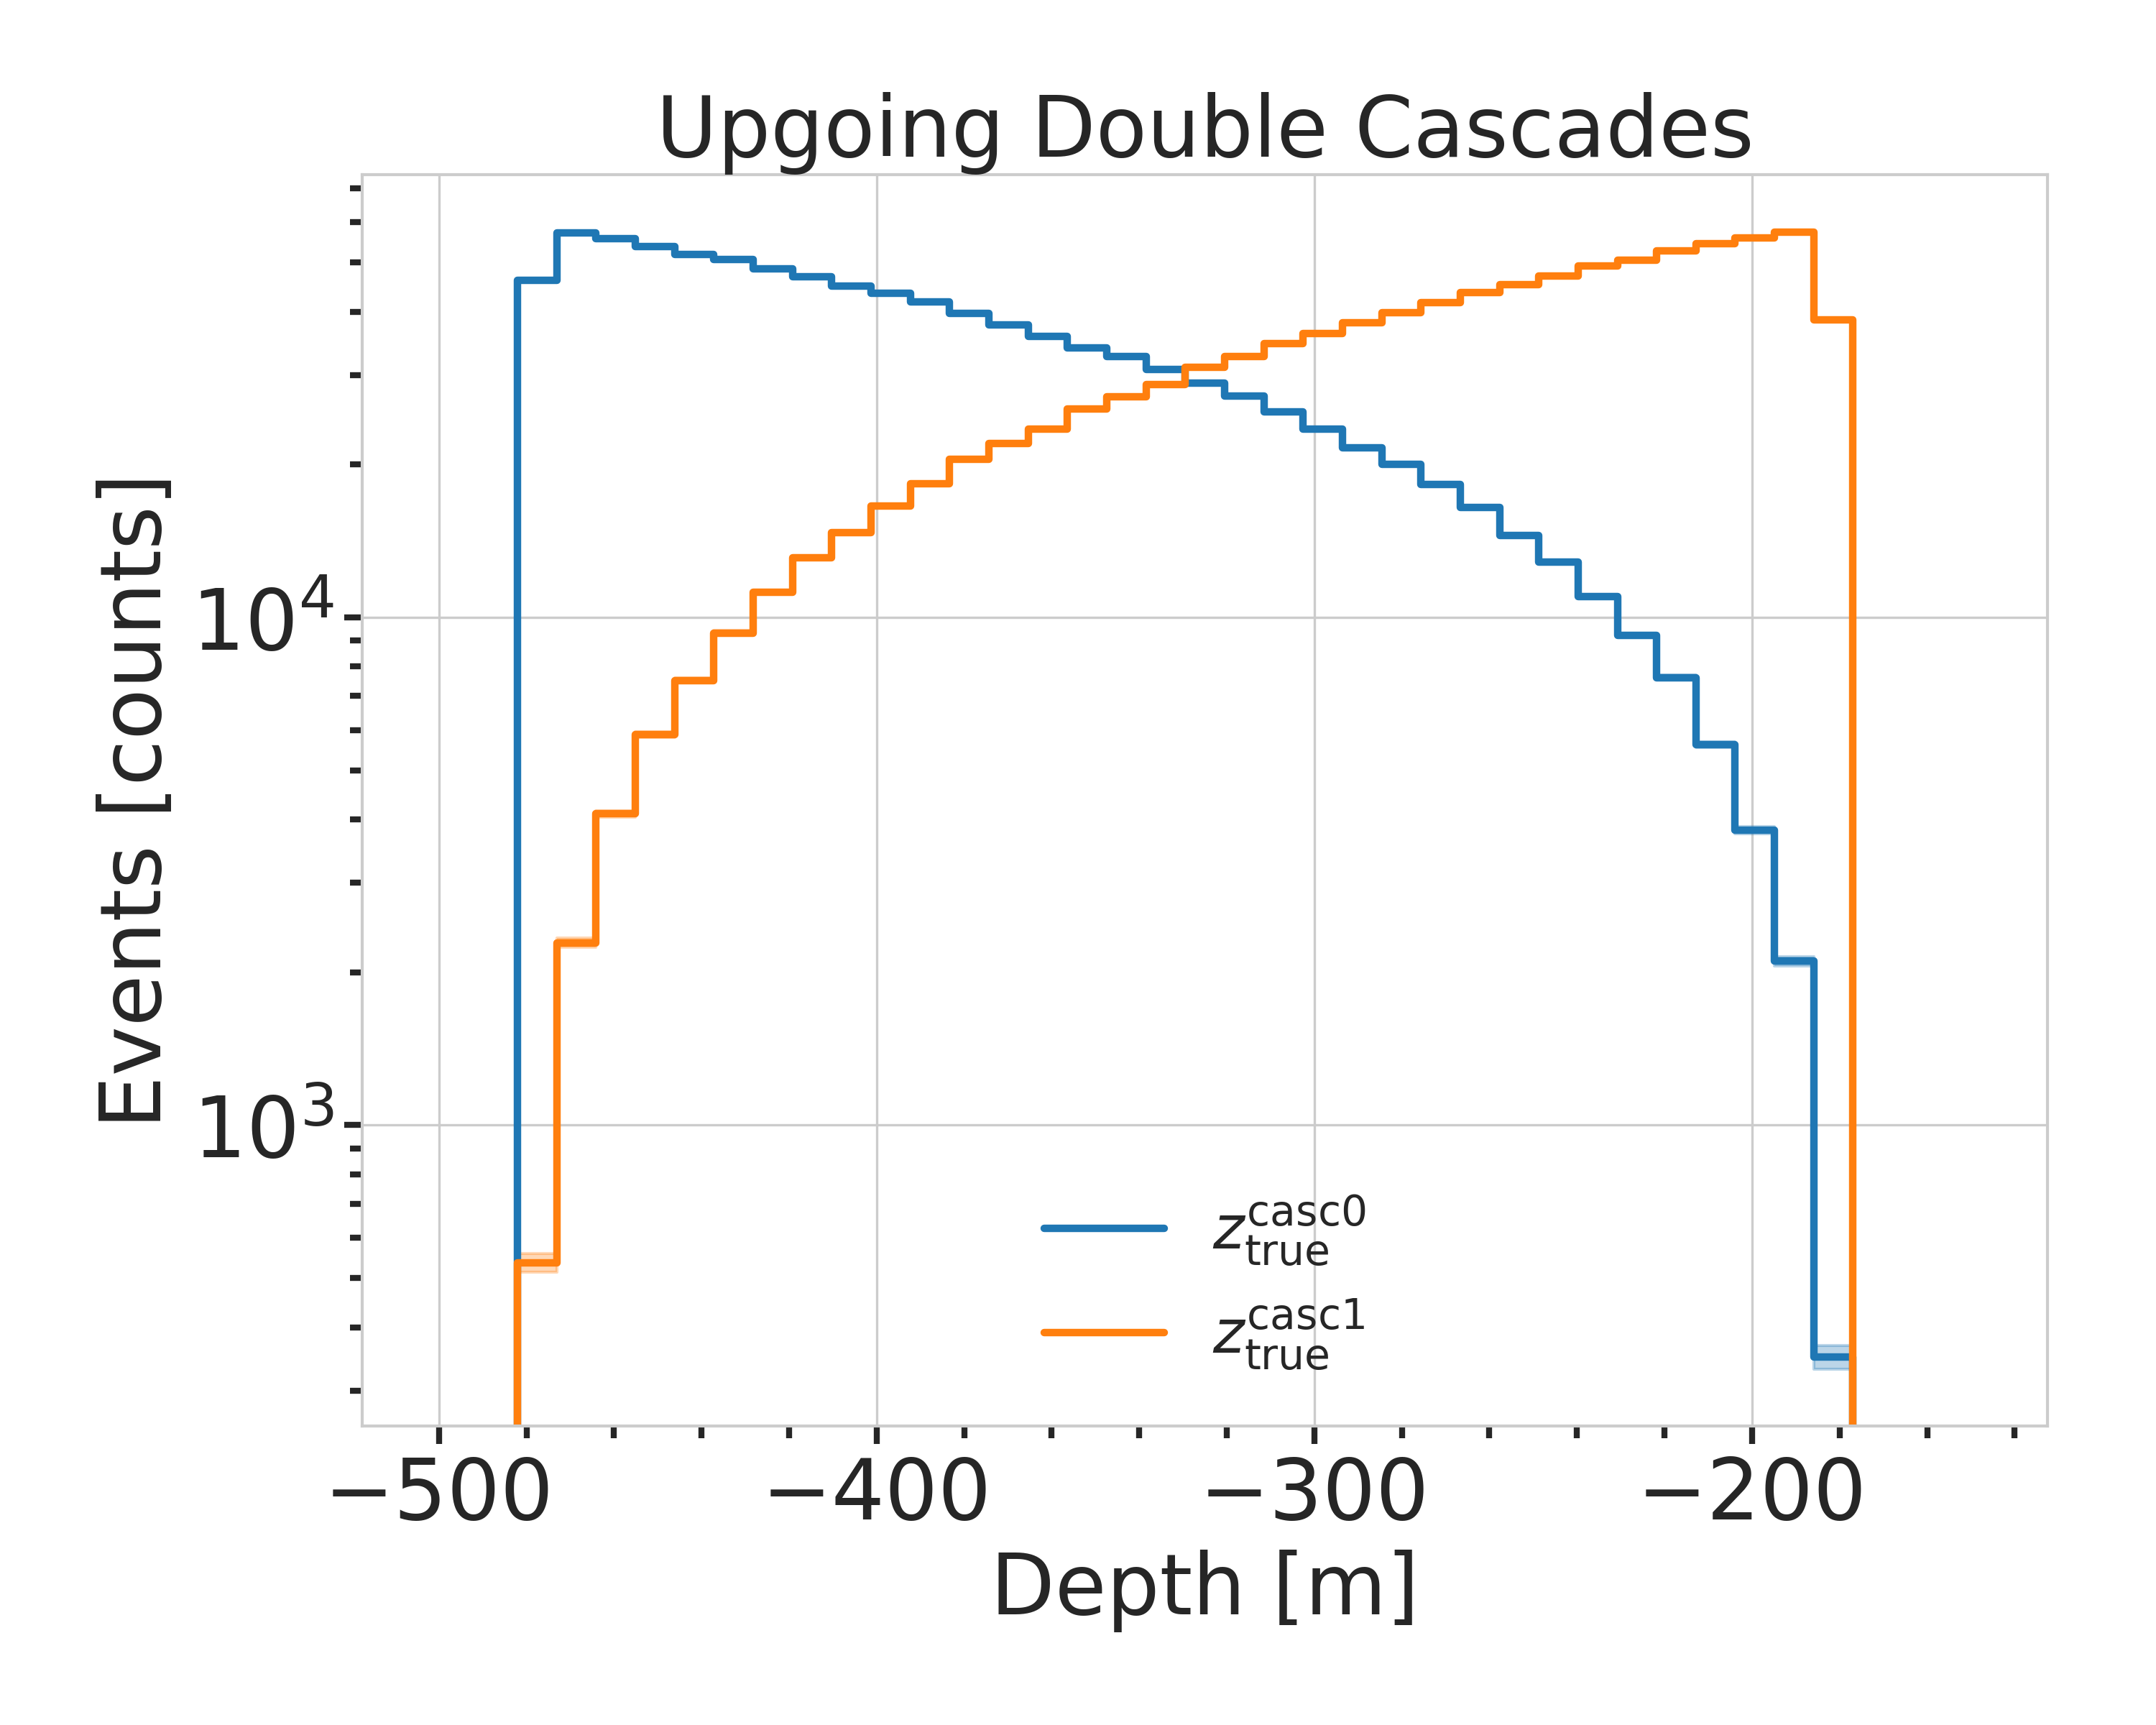
\includegraphics[width=.45\linewidth]{figures/upgoing_string_81_gen_level/1_d_distr_depths_clipped.png}
%     }
%     \\[-2.5ex]
%     \subfloat[\labfig{horizontal_gen_distris_decay_length}]{
%         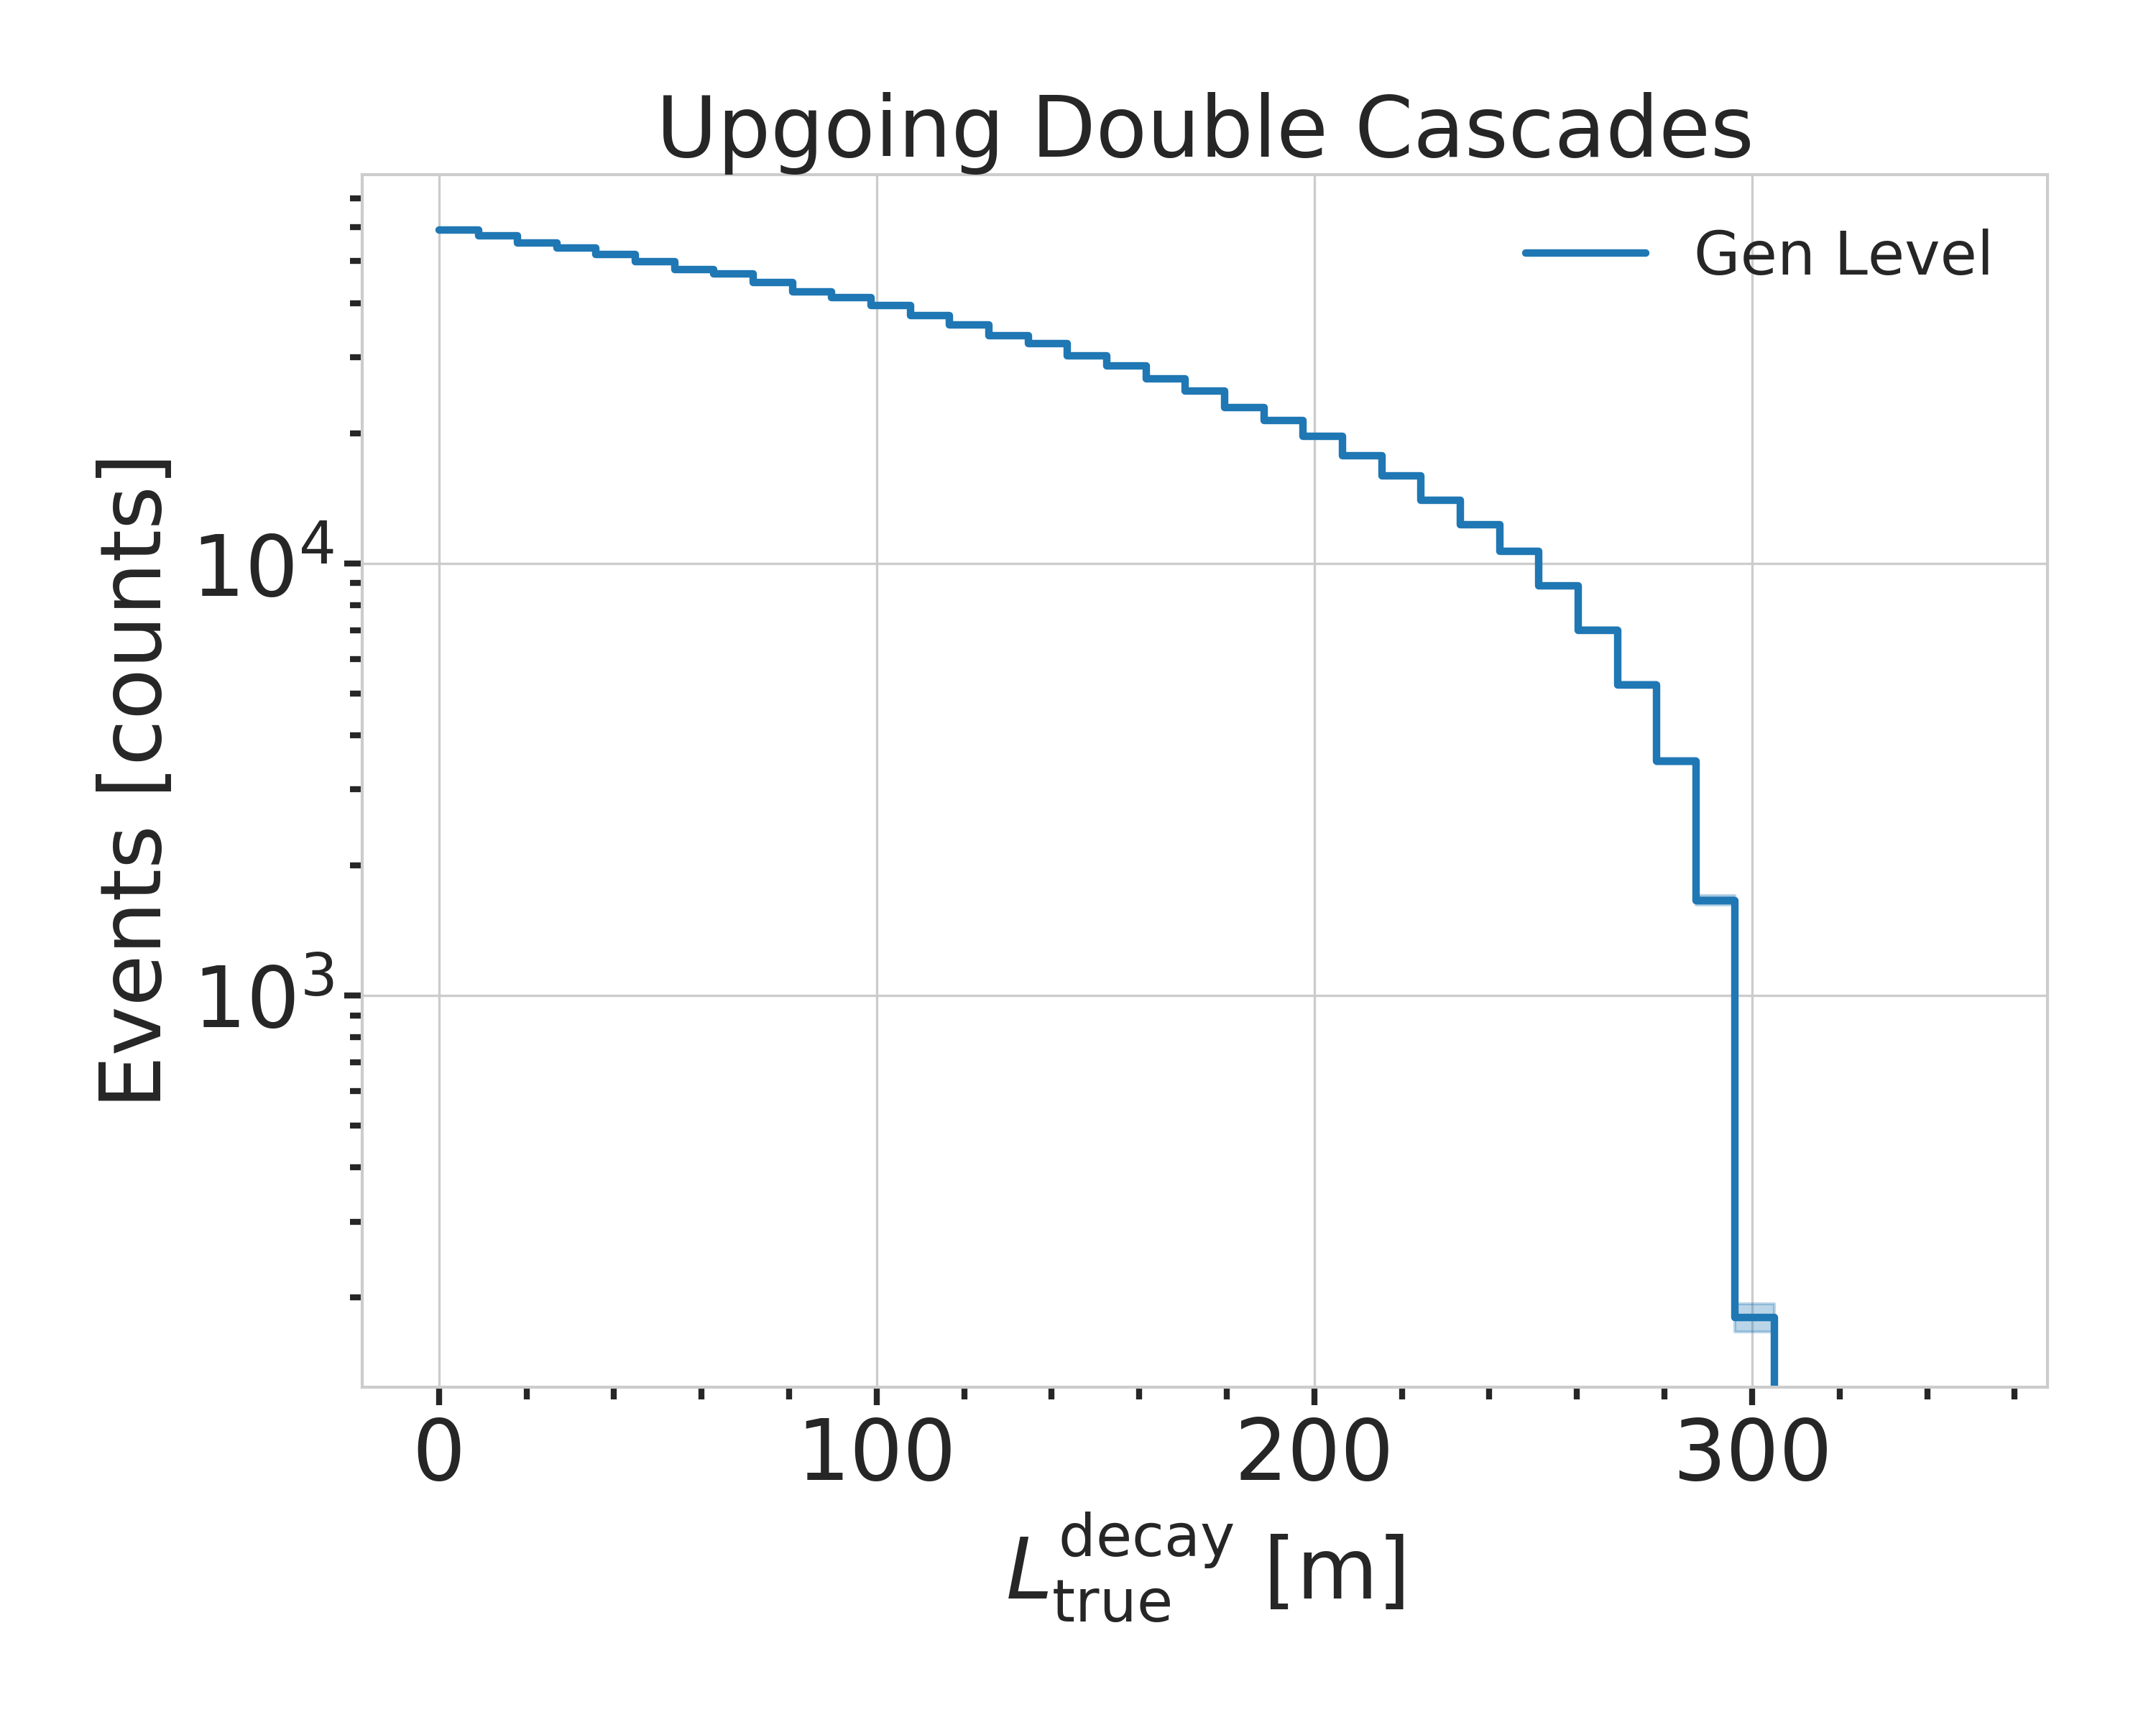
\includegraphics[width=.45\linewidth]{figures/upgoing_string_81_gen_level/1_d_distr_true_decay_length_clipped.png}
%     }
%     \subfloat[\labfig{horizontal_gen_distris_total_energy}]{
%         \includegraphics[width=.45\linewidth]{figures/upgoing_string_81_gen_level/1_d_distr_true_total_energy_clipped.png}
%     }
%     \caption{Generation level distributions of the 1k files, with 1k events each of set 194601. Only the parameters that are not fixed to a certain value are shown.}
%     \labfig{horizontal_gen_distris}
% \end{figure}



\subsection{Realistic Set}



\section{Model Specific Simulation} \labsec{model_specific_simulation}

\todo{Re-write/re-formulate this section (copied from HNL technote).}


\subsection{Custom LeptonInjector} \labsec{custom_leptoninjector}

Signal events are simulated using a \href{https://github.com/LeanderFischer/LeptonInjector-HNL/tree/main/LeptonInjector}{custom LeptonInjector (LI) tool} \sidecite{IceCube:2020tcq}, modified from its standard version to include the HNL particle and the description of the HNL decays needed to produce the double cascade signature (currently only $\nu_{\tau}$ related). In its SM work mode, LI injects a lepton and a cascade (under the general name \textit{Hadrons}) at the interaction vertex of the neutrino. Both objects have the same (x,y,z,t) coordinates. In the modified version, the lepton at the interaction vertex is replaced by the HNL. After a chosen distance the HNL is forced to decay. The decay is sampled from the kinematically accessible decay modes shown in \reffig{hnl_decay_modes_log_branching_ratio}.

A big addition to the standard LI is that the decay products of the HNL are added to the list of particles in the I3MCTree with a displaced position and delayed time from the interaction vertex. These daughter particles form a second cascade, not in the form of a \textit{Hadrons} object, but as the explicit particles forming the shower. The kinematics of the two-body decays are computed analytically, while the three-body decays are dealt with using MadGraph5. To do so, we randomly pick an event from a list that we generated for each three-body decay mode. Independent of the number of particles in the final state of the HNL decay, the kinematics are calculated/simulated at rest and then boosted along the HNL momentum. The decay mode is randomly chosen based on the mass dependent branching ratios shown in \reffig{hnl_decay_modes_log_branching_ratio}.

Each file is produced by running the \href{https://github.com/LeanderFischer/I3_HNL_Decay/blob/master/submission_scripts/process/process_Gen.py}{generation level processing script} using the filenumber as random seed and the above settings for the sampling distributions. The main part is calling the \textit{MultiLeptonInjector} module in \textit{volume mode} adding two generators (for $\nu_\tau$ and $\bar{\nu}_\tau$) with $50\%$ of the events. The generators are provided with the custom double-differential/total cross section splines described in \refsec{hnl_cross_sections} and the parameters defining the sampling distributions. For each frame \textit{OneWeight} and a reference weight are also calculated and stored using the \href{https://github.com/LeanderFischer/LeptonInjector-HNL/blob/main/LeptonInjector/python/hnl_weighting.py}{weighting functions} and a baseline atmospheric $\nu_\tau$ flux + oscillation spline. The weight will later be calculated inside of the analysis framework \href{https://github.com/icecube/pisa}{PISA}, based on the input OneWeight. In addition to the i3 file itself, a LeptonInjector configuration file is written which stores the needed information to produce event weights using LeptonWeighter. Optionally the script can also produce an hdf5 file with the same name in the same location. This will store a fixed set of keys, extracted from the i3 file.

We are using \textit{volume mode}, for the injection of the primary particle on a cylindrical volume. The main generation/sampling happens in \texttt{VolumeLeptonInjector::DAQ} inside \\ \texttt{LeptonInjector.cxx}. After writing the config (s) frame (currently not kept), the energy is sampled from a power law distribution, then the cosine(zenith) and azimuth angles are sampled from uniform distributions. The (x,y) position is sampled uniform in $r, \phi$ (for position on disk) and the z position is sampled from a uniform distribution. After the primary properties have been sampled the \textit{EventProperties} is created and handed over to the \texttt{FillTree} functions which is where the custom HNL simulation happens:

\subsubsection{Cross Sections} \labsec{hnl_cross_sections}


\todo{add varied total cross-section for a few background HNL events}

\begin{figure}
    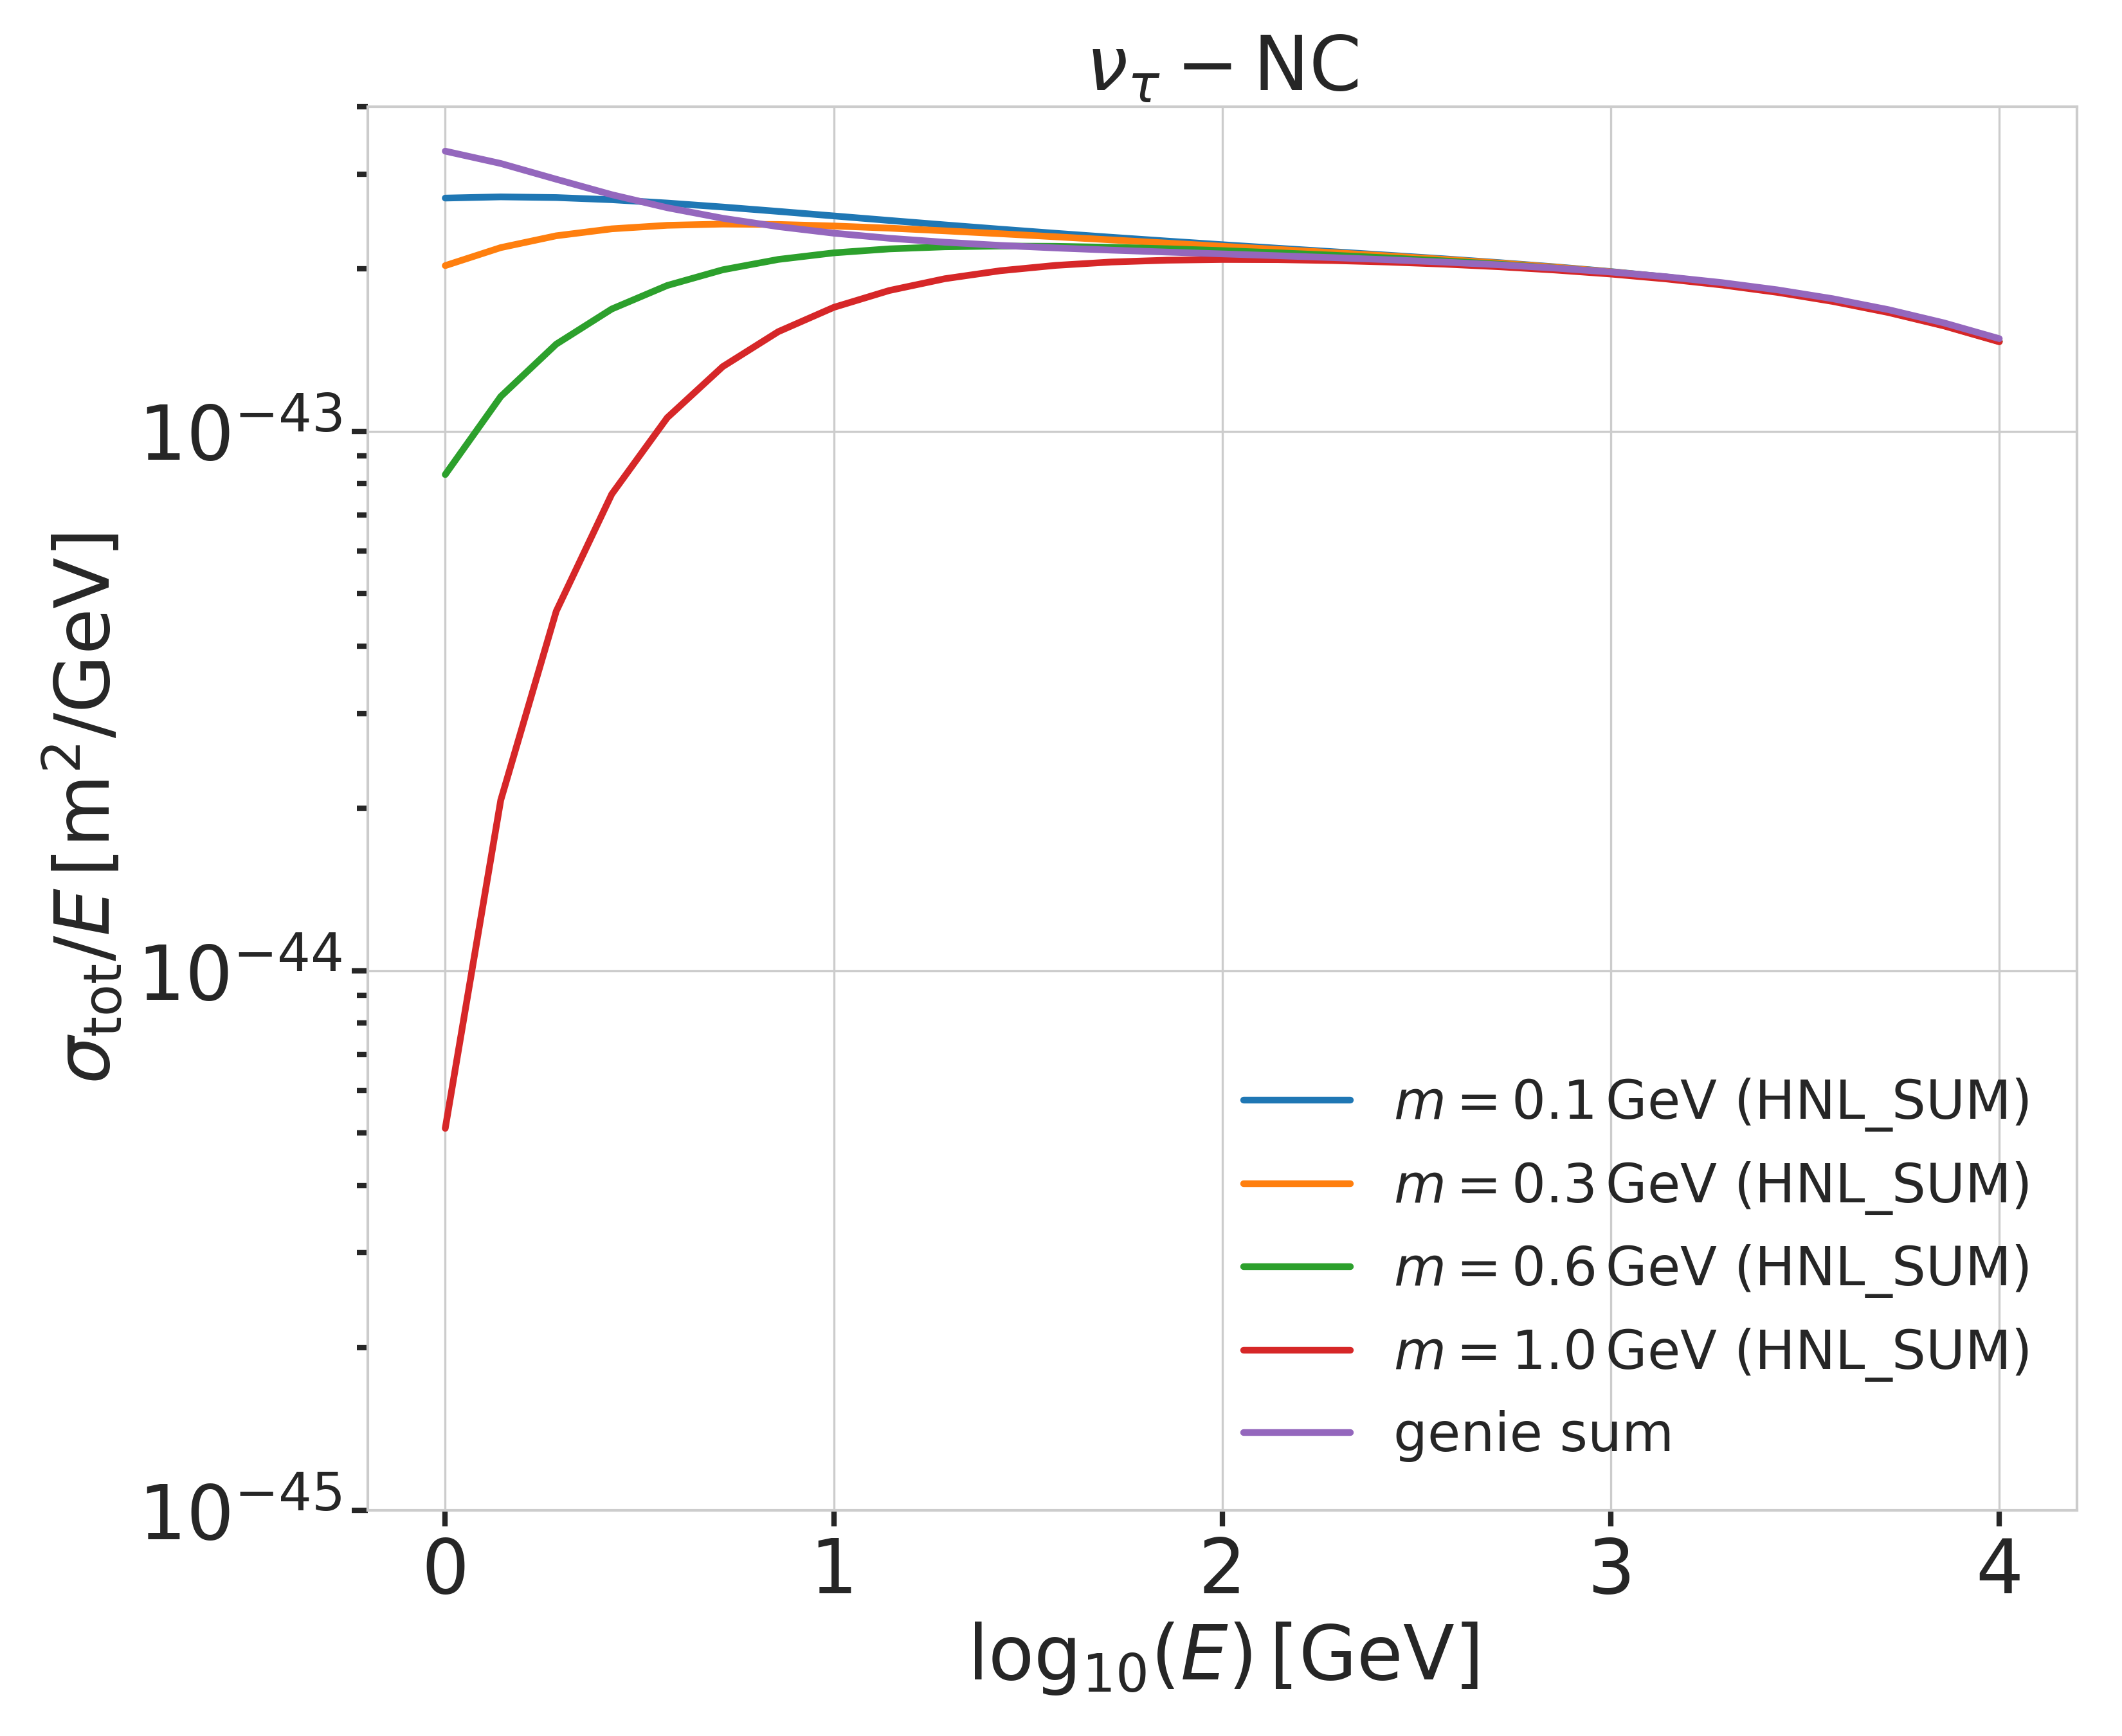
\includegraphics[width=.49\linewidth]{figures/hnl_simulation/cross_sections/custom_HNL_xsecs_final_SUM_flavorwise_total_xsecs_sigma-nutau-N-nc.png}
    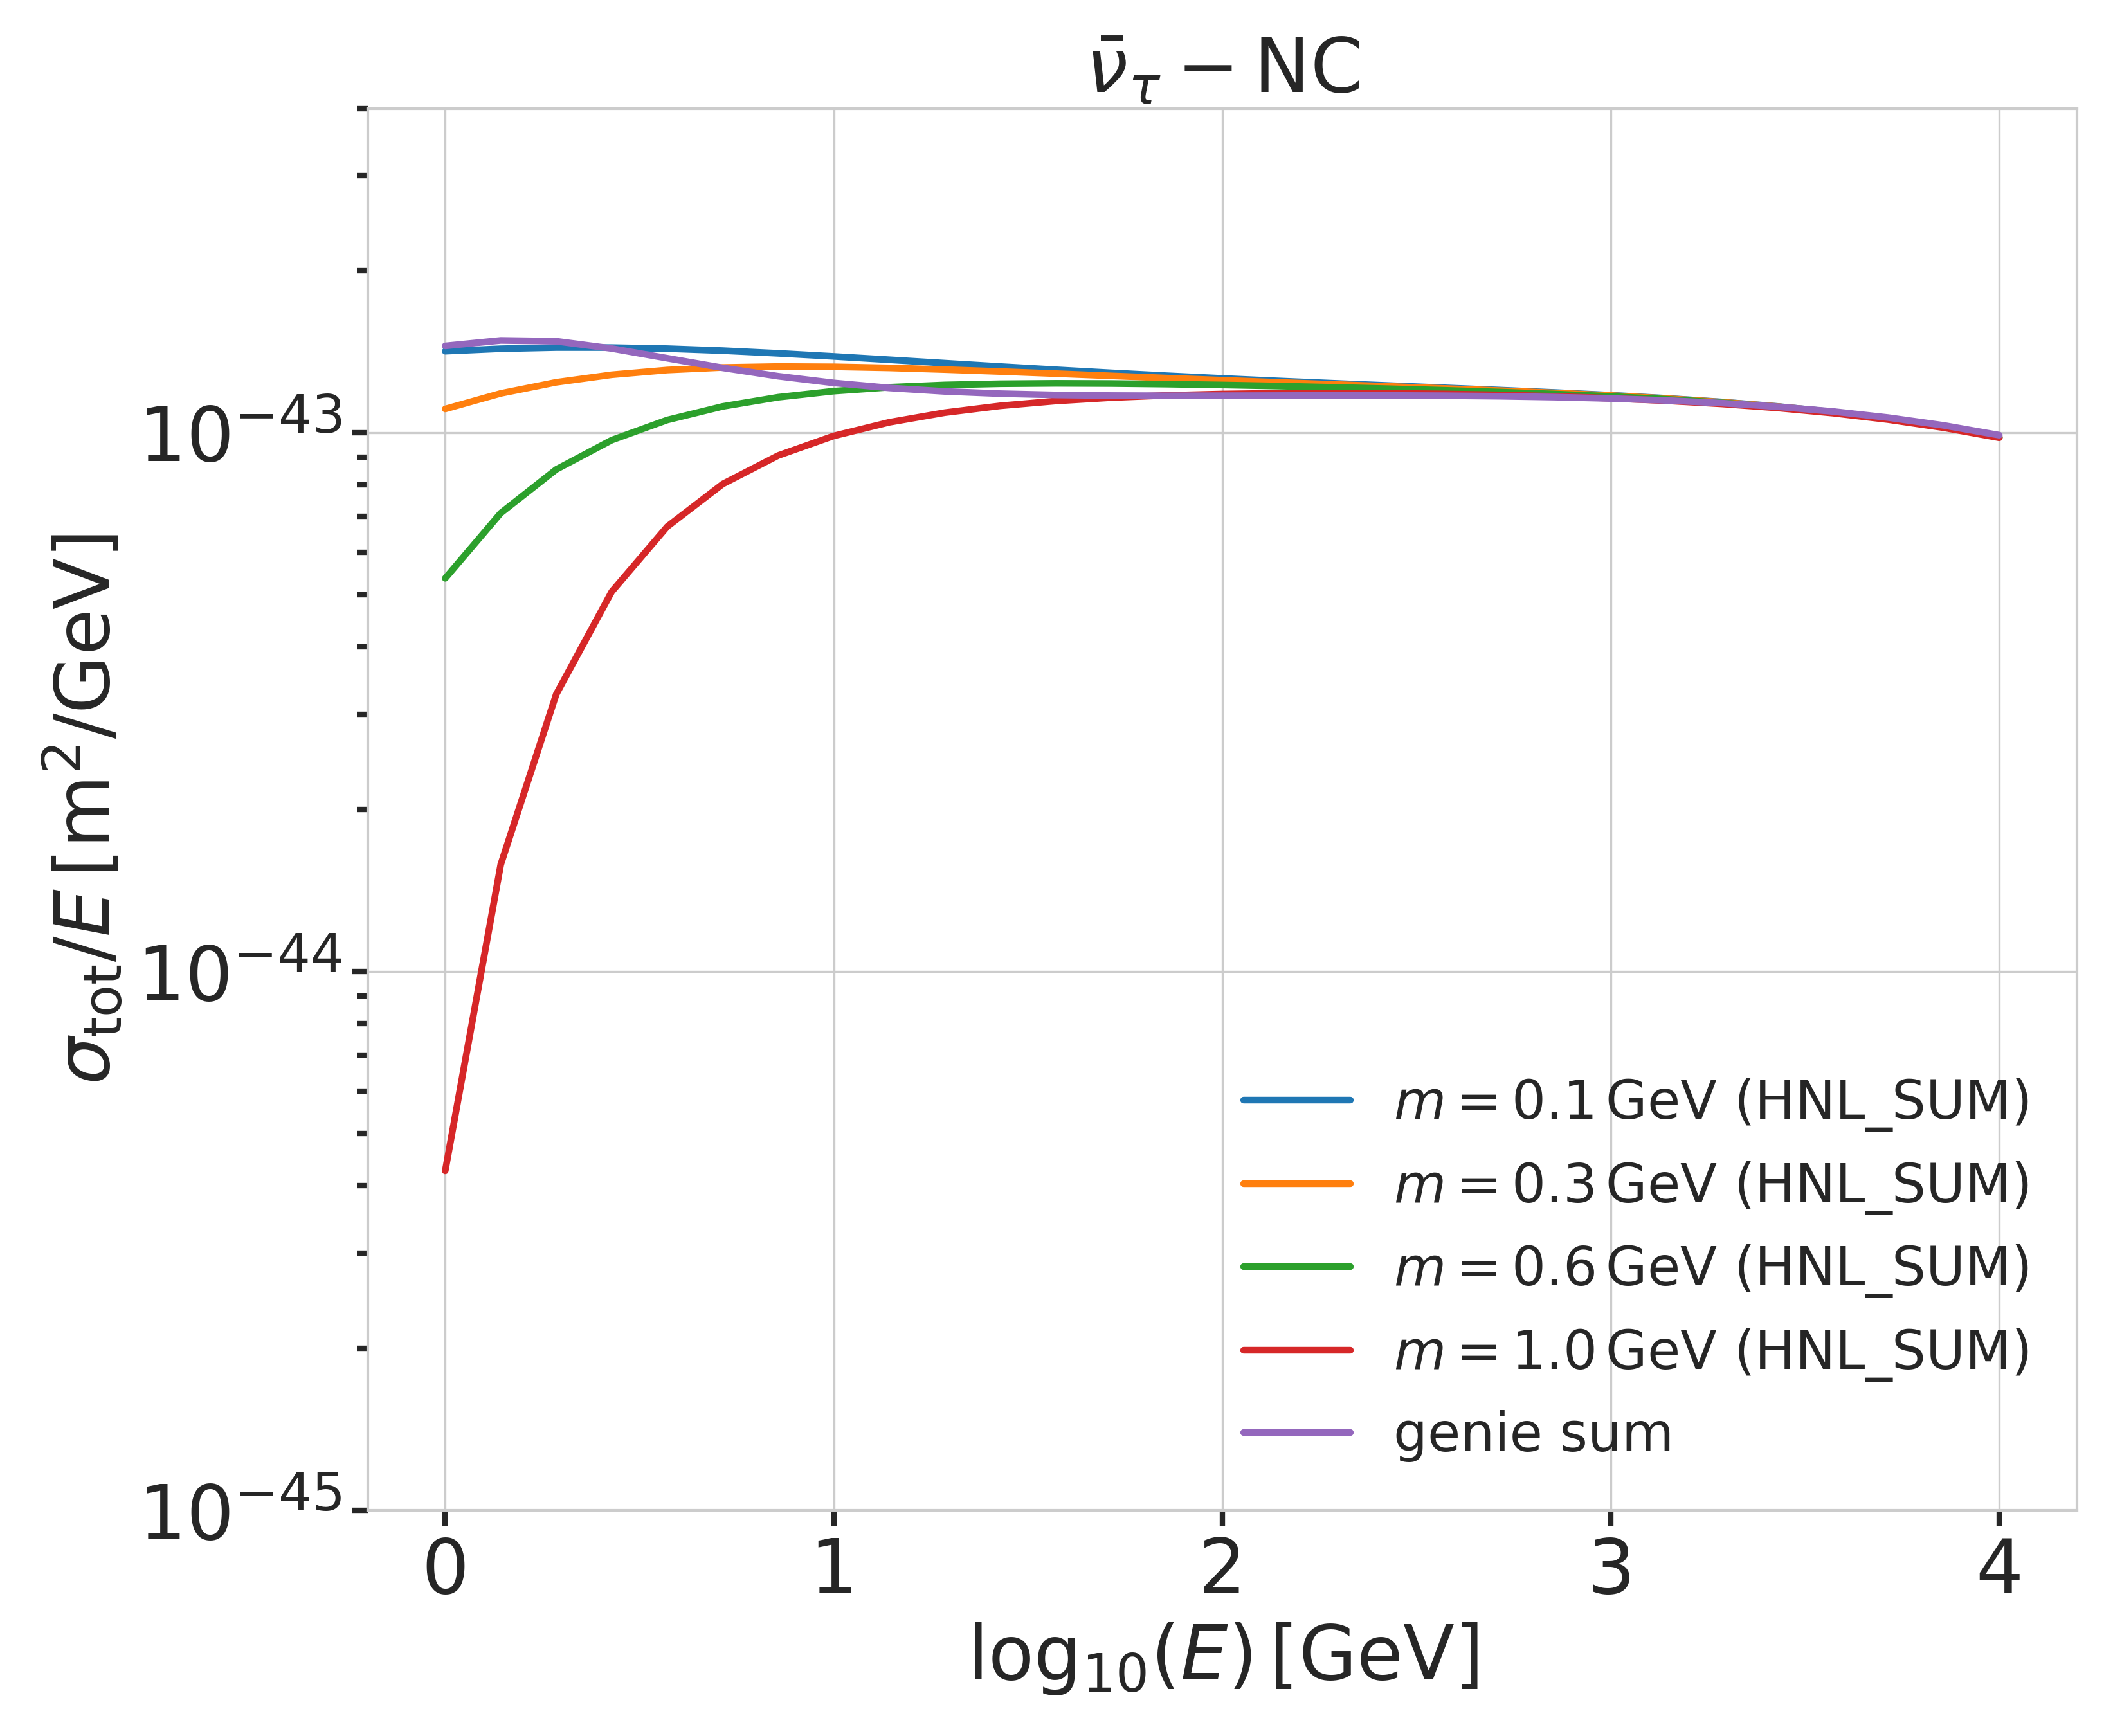
\includegraphics[width=.49\linewidth]{figures/hnl_simulation/cross_sections/custom_HNL_xsecs_final_SUM_flavorwise_total_xsecs_sigma-nutaubar-N-nc.png}
    \caption{Custom HNL total cross sections for the four target masses compared to the total ($\nu_\tau$/$\bar{\nu}_\tau$ neutral current) cross section used for SM neutrino simulation production with GENIE.}
    \labfig{custom_hnl_cross_sections}
\end{figure}

The cross sections are calculated using a \href{https://github.com/LeanderFischer/NuXSSplMkr/tree/massive_nu_nc_dis}{modified version} of Carlos Argüelles' \href{https://github.com/arguelles/NuXSSplMkr}{NuXSSplMkr}, which is a tool to calculate neutrino cross sections from parton distribution functions (PDFs) and then produce splines that can be read and used with IceCube software. The main modification to calculate the cross sections for the $\nu_\tau$ neutral current interaction into the new heavy mass state is the addition of a kinematic condition to ensure that there is sufficent energy to produce the heavy mass state. It is the same confition that needs to be fulfilled for the charged current case, where the outgoing lepton mass is non-zero. Following \sidecite{Levy:2004rk} (equation 7), the condition
\begin{equation}
    (1 + x \delta_N) h^2 - (x + \delta_{4}) h + x \delta_{4} \leq 0,
\end{equation}
is implemented for the neutral current case. Here $\delta_{4}=\frac{m_4^2}{s-M^2}$, $\delta_{N}=\frac{M^2}{s-M^2}$, and $h \overset{\textit{def}}{=} xy + \delta_{4}$, with $x, y$ being the Bjorken variables, $m_4$ and $M$ the mass of the heavy state and the target nucleon, respectively, and $s$ the center of mass energy squared. Since the (SM) neutrino background simulation used for this analysis was created using GENIE (version 2.12.8), interfaced through the IceCube software package \textit{genie-icetray}, with the \href{https://internal.dunescience.org/doxygen/classgenie_1_1GRV89LO.html}{GRV98LO} PDFs, those were added as \textit{GRV98lo\_patched} to the cross section spline maker, to ensure the best possibe agreement. Double-differential ($dsdxdy$) and total ($\sigma$) cross sections were produced for the four target HNL masses and then splined. The produced cross section splines are stored \href{https://github.com/LeanderFischer/LeptonInjector-HNL/tree/main/LeptonInjector/resources/cross_sections}{in the resources of the custom LeptonInjector module}. \reffig{custom_hnl_cross_sections} shows the total cross sections that were produced compared to the cross section used for the production of the SM $\nu_\tau/\bar{\nu}_\tau$ neutral current background simulation \todo{Add comparions of SM cross sections between NuXSSplMkr and genie}.


\subsubsection{Decay Channels}

\begin{figure}
    \includegraphics{hnl_simulation/decay_theory/branching_ratios_log_up_to_1.0_GeV.png}
    \caption{Branching ratios of the HNL within the mass range considered, calculated based on the results from \cite{Coloma:2020lgy}. Given the existing constraints on $|U_{e4}|^{2}$ and $|U_{\mu4}|^{2}$, we consider that the corresponding decay modes are negligible.}
    \labfig{hnl_decay_modes_log_branching_ratio}
\end{figure}

The accessible decay channels are dependent on the mass of the HNL and the allowed mixing. For this analysis, where only $|U_{\tau4}|^2 \neq 0$, the considered decay channels are listed in \reftab{hnl_decay_channels} and the corresponding branching ratios are shown in \reffig{hnl_decay_modes_log_branching_ratio}. The indiviudal branching ratio for a specific mass is calculated as $\mathrm{BR}_i(m_4)=\Gamma_i(m_4)/\Gamma_\mathrm{total}(m_4)$, where $\Gamma_\mathrm{total}(m_4)=\sum\Gamma_i(m_4)$. The formulas to calculate the decay width show up in multiple references, but we chose to match them to \sidecite{Coloma:2020lgy}, which also discusses the discrepencies in previous literature.

\begin{margintable}
    \footnotesize
    \begin{tabular} { lll }
        \hline\hline 
        \textbf{Channel} & \textbf{Opens} & \textbf{$\hat{\mathrm BR}$ [\%]} \\
        \hline\hline 
        $\nu_4 \rightarrow \nu_\tau \nu_\alpha \bar{\nu_\alpha}$ & \SI{0}{\MeV} & 100.0 \\
        $\nu_4 \rightarrow \nu_\tau e^+ e^-$ & \SI{1}{\MeV} & ? \\
        $\nu_4 \rightarrow \nu_\tau \pi^0$ & \SI{135}{\MeV} & ? \\
        $\nu_4 \rightarrow \nu_\tau \mu^+ \mu^-$ & \SI{211}{\MeV} & ? \\
        $\nu_4 \rightarrow \nu_\tau \eta$ & \SI{548}{\MeV} & ? \\
        $\nu_4 \rightarrow \nu_\tau \rho^0$ & \SI{770}{\MeV} & ? \\
        $\nu_4 \rightarrow \nu_\tau \omega$ & \SI{783}{\MeV} & ? \\
        $\nu_4 \rightarrow \nu_\tau \eta'$ & \SI{958}{\MeV} & ? \\
        \hline
    \end{tabular}
    \caption[xx]{xx}
    \labtab{hnl_decay_channels}
\end{margintable}



\paragraph{2-Body Decay Widths}

The decay to a neutral pseudoscalar mesons is
\begin{equation}
    \Gamma_{\nu_4 \rightarrow \nu_\tau P} = |U_{\tau4}|^2 \frac{G_F^2 m_4^3}{32\pi} f_P^2 (1-x_p^2)^2,
    \labeq{gamma_nu_P}
\end{equation}
with $x_P = m_P/m_4$ and
\begin{equation}
    f_{\pi^0} = \SI{0.130}{\GeV}, \hspace{1cm} f_{\eta} = \SI{0.0816}{\GeV}, \hspace{1cm} C_2 = f_{\eta'} = \SI{-0.0946}{\GeV},
    \labeq{gamma_nu_P_f_factors}
\end{equation}
while the decay to a neutral vector meson is given by
\begin{equation}
    \Gamma_{\nu_4 \rightarrow \nu_\tau V} = |U_{\tau4}|^2 \frac{G_F^2 m_4^3}{32\pi} \bigg(\frac{f_V}{m_V}\bigg)^2 g_V^2 (1+2x_V^2) (1-x_V^2)^2,
    \labeq{gamma_nu_V}
\end{equation}
with $x_V = m_V/m_4$,
\begin{equation}
    f_{\rho^0} = \SI{0.171}{\square\GeV}, \hspace{1cm} f_{\omega} = \SI{0.155}{\square\GeV},
    \labeq{gamma_nu_V_f_factors}
\end{equation}
and
\begin{equation}
    g_{\rho^0} = 1-2\sin^2{\theta_w}, \hspace{1cm} g_{\omega} = \frac{-2\sin^2{\theta_w}}{3}, \hspace{1cm} \sin^2{\theta_w} = 0.2229
    \labeq{gamma_nu_V_g_factors}
\end{equation}
\sidecite{codata2018}.


\paragraph{3-Body Decay Widths}

The (invisible) decay to three neutrinos is
\begin{equation}
    \Gamma_{\nu_4 \rightarrow \nu_\tau \nu_\alpha \bar{\nu_\alpha}} = |U_{\tau4}|^2 \frac{G_F^2 m_4^5}{192\pi^3},
    \labeq{gamma_nu_nu_nu}
\end{equation}
while the decay to two charged leptons (using $x_\alpha = (m_\alpha/m_4)^2)$ of the same flavor reads
\begin{equation}
    \Gamma_{\nu_4 \rightarrow \nu_\tau l_\alpha^+ l_\alpha^-} = |U_{\tau4}|^2 \frac{G_F^2 m_4^5}{192\pi^3} \big[ C_1 f_1(x_\alpha) + C_2 f_2(x_\alpha) \big],
    \labeq{gamma_nu_ll_full}
\end{equation}
with the constants defined as
\begin{equation}
    C_1 = \frac{1}{4}(1-4s_w^2+8s_w^4) , \hspace{1cm} C_2 = \frac{1}{2}(-s_w^2+2s_w^4),
    \labeq{gamma_nu_ll_c1_c2}
\end{equation} 
the functions as
\begin{equation}
    f_1(x_\alpha) = (1-14x_\alpha-2x_\alpha^2-12x_\alpha^3)\sqrt{1-4x_\alpha}+12x_\alpha^2(x_\alpha^2-1)L(x_\alpha),
    \labeq{gamma_nu_ll_f1}
\end{equation}
\begin{equation}
    f_2(x_\alpha) = 4[x_\alpha(2+10x_\alpha-12x_\alpha^2)\sqrt{1-4x_\alpha}+6x_\alpha^2(1-2x_\alpha+2x_\alpha^2)L(x_\alpha)],
    \labeq{gamma_nu_ll_f2}
\end{equation}
and
\begin{equation}
    L(x) = \ln \biggl( \frac{ 1-3x_\alpha-(1-x_\alpha)\sqrt{1-4x_\alpha} }{ x_\alpha(1+\sqrt{1-4x_\alpha}) } \biggr).
    \labeq{gamma_nu_ll_l}
\end{equation}


\subsection{MadGraph5 3-Body Decays} \labsec{madgraph_3body_decays}

The code to produce the 3-body decay kinematics is \href{https://launchpad.net/mg5amcnlo/3.0/3.3.x}{MadGraph4 v3.4.0} based on the decay diagrams calculated with \href{http://feynrules.irmp.ucl.ac.be/#FeynRules2.0}{FeynRules 2.0} using the Lagrangians derived in \sidecite{Coloma:2020lgy}. The Universal FeynRules Outpur (UFO) from \texttt{effective\_HeavyN\_Majorana\_v103} were used for our calculation. For each meass and corresponding decay channel, we produce $1e06$ decay kinematic variations (rest frame) and store those in a text file. 


\subsection{Sampling Distributions}

This is the description of the signal simulation generator used to (re-)start simulation production in December 2023. The underlying sampling distributions are listed in \reftab{HNL_sampling_distributions}. Judging from how the generation/processing efficiency was for the 190607 set, we target $1e04$ files per set with $5e05$ events per file at generation, resulting in a maximum of $5e09$ events per set at generation level. Note here that the actual number of events per set at generation might be a little lower since some events won't be allowed if they don't have enough energy to produce the HNL.

\begin{table}
    \centering
    \begin{tabular} { lll }
        \hline \hline 
        \textbf{Variable} & \textbf{Distribution} & \textbf{Range/Value} \\
        \hline \hline 
        energy & $E^{-2}$ & [\SI{2}{\GeV}, \SI{1e4}{\GeV}] \\
        zenith & uniform (in $\cos(\theta)$) & [\SI{180}{\degree}, \SI{80}{\degree}] \\
        azimuth & uniform & [\SI{0}{\degree}, \SI{360}{\degree}] \\
        vertex ($x,y$) & uniform & $r$=\SI{600}{\metre} \\
        vertex $z$ & uniform & [-600, 0]\si{\metre} \\
        $m_\mathrm{4}$ & fixed & [0.3, 0.6, 1.0]\si{\GeV} \\
        $L_\mathrm{decay}$ & $L^{-1}$ & [0.0004, 1000]\si{\metre} / [1, 1000]\si{\metre} \\
        \hline
    \end{tabular}
    \caption[xx]{Sampling distributions of HNL simulation generation.}   
    \labtab{hnl_realistic_set_sampling_distributions}
\end{table}


\subsection{Weighting Scheme}

The weighting for the HNL signal simulation happens in a \href{https://github.com/icecube/pisa/blob/master/pisa/stages/aeff/weight_hnl.py}{custom stage of PISA}. The only input is the stored OneWeight and the variable physics parameter $|U_{\tau4}|^2$, which is the mixing strength of the new heavy mass state and the tau sector. The custom re-weighting is needed to go from the used sampling PDF (1/L with fixed range in lab frame decay length) to the target PDF (exponential defined by proper lifetime of the HNL). For each event the re-weighting factor is calculated using the gamma factor
\begin{equation}
    \gamma = \frac{\sqrt{E_\mathrm{kin}^2+m_\mathrm{HNL}^2}}{m_\mathrm{HNL}},
    \labeq{gamma_factor}
\end{equation}
with the HNL mass $m_\mathrm{HNL}$ and it's kinetic energy $E_\mathrm{kin}$. The speed of the HNL is calculated as
\begin{equation}
    v = c \cdot \sqrt{1 - \frac{1}{\gamma^2}},
    \labeq{lorentz_speed}
\end{equation}
where $c$ is the speed of light. With these the lab frame decay length range can be converted into the rest frame lifetime range for each event
\begin{equation}
    \tau_\mathrm{min/max} = \frac{s_\mathrm{min/max}}{v\cdot\gamma}.
\end{equation}
The proper lifetime of each HNL event can be calculated using the total decay width $\Gamma_\mathrm{total}$ shown in \reffig{hnl_decay_modes_log_decay_width} and the chosen mixing strength $|U_{\tau4}|^2$ as
\begin{equation}
    \tau_\mathrm{proper} = \frac{\hbar}{\Gamma_\mathrm{total}(m_\mathrm{HNL}) \cdot |U_{\tau4}|^2},
    \labeq{proper_lifetime}
\end{equation}
where $\hbar$ is the reduced Planck constant. Since the decay length/lifetime of the events is sampled from an inverse distribution instead of an exponential as it would be expected from a particle decay we have to re-weight accordingly to achieve the correct decay length/lifetime distribution. This is done by using the wanted exponential distribution
\begin{equation}
    \mathrm{PDF}_\mathrm{exp} = \frac{1}{\tau_\mathrm{proper}} \cdot e^{\frac{-\tau}{\tau_\mathrm{proper}}},
    \labeq{pdf_exponential}
\end{equation}
and the inverse distribution that was sampled from
\begin{equation}
    \mathrm{PDF}_\mathrm{inv} = \frac{1}{\tau \cdot (\ln(\tau_\mathrm{max}) - \ln(\tau_\mathrm{min}))}.
    \labeq{pdf_inverse}
\end{equation}
The lifetime re-weighting factor is calculated as
\begin{equation}
    w_\mathrm{lifetime} = \frac{\mathrm{PDF}_\mathrm{exp}}{\mathrm{PDF}_\mathrm{inv}} = \frac{\Gamma_\mathrm{total}(m_\mathrm{HNL}) \cdot |U_{\tau4}|^2}{\hbar} \cdot \tau \cdot (\ln(\tau_\mathrm{max}) - \ln(\tau_\mathrm{min})) \cdot e^{\frac{-\tau}{\tau_\mathrm{proper}}}.
    \labeq{weight_lifetime}
\end{equation}
Adding another factor of $|U_{\tau4}|^2$ to account for the mixing at the interaction vertex the total re-weighting factor becomes
\begin{equation}
    w_\mathrm{total} = |U_{\tau4}|^2 \cdot w_\mathrm{lifetime},
    \labeq{weight_full}
\end{equation}
which can be applied on top of flux and oscillation weight to get the final HNL weight for a given mixing (and mass).

\section{Model Dependent Simulation Distributions}

\subsection{Generation Level}

\subsection{Final Level}


% \setchapterstyle{kao}
\setchapterpreamble[u]{\margintoc}

\todo{maybe increase main text width? (read in kao docu)}
\todo{Adapt to reflect switched chapter order}

\chapter{Standard Model Background Simulation and Data Processing}
\labch{simulation_and_processing}

The analysis presented in this thesis is highly dependent on an efficient event selection to reduce the raw IceCube trigger data to a usable atmospheric neutrino sample. Based on this selection, a precise estimation of both expected SM background and expected BSM signal events can be made using MC simulations. This chapter describes the current simulation and event selection chain used for state-of-the-art IceCube neutrino oscillation measurements like \sidecite[0.3cm]{OVS_PRD}. The whole chain can be broadly split into 4 steps:

\begin{enumerate}[wide]
    
    \item[]{\textbf{Step 1 Event Generation:}} The initial step for all particle (non-noise) simulation is the generation of events from selected initial distributions and fluxes. Events are the primary particle and the particles produced in the interaction with the ice.
    \vspace{0.2cm} 

    \item[]{\textbf{Step 2 Detector Simulation:}} The particles from the first step are propagated through the ice, producing Cherenkov photons, which are then propagated further until they reach a DOM or are absorbed. If they hit a DOM the detector response (acceptance and PMT) is simulated.
    \vspace{0.2cm} 
        
    \item[]{\textbf{Step 3 Processing:}} Starting from the PMT output, both real data and simulation are processed through the in-ice trigger, the online filter and processing, and the low energy event selection to produce a neutrino dominated sample.
    \vspace{0.2cm} 

    \item[]{\textbf{Step 4 Reconstruction:}} Once the sample is small enough for more sophisticated reconstruction techniques to be feasible to run, the events are reconstructed using a CNN and some high level variables are computed. Based on these variables the final event selection is applied.
    
\end{enumerate}

This chapter only describes the event generation for the SM background simulation (neutrinos and muons), while the signal simulation is described in \refch{signal_simulation}. The detector simulation is identical for both signal and background events while processing and reconstruction are applied to all simulation and data in the same way. Splitting the simulation steps has the advantage of reusing the outputs of for example the generation step to propagate the particles with different ice model, in order to estimate the systematic impacts of uncertainties of the ice properties. Similar approach can be taken for varying detector response and through this a more efficient (reduced) use of computing resources can be achieved. The following sections describe the different steps in more detail and the last section, \refsec{systematic_uncertainties}, describes the related systematic uncertainties considered for this work.


\section{Event Generation} \labch{sm_event_generation}

The MC is used in the analysis by applying a method called \textit{forward folding}, where a very large number of events (signal and background) is produced using sampling distribution that are tuned to have a large selection efficiency. Those distributions don't have to be physically correct distributions, but they need to cover the full parameter space of interest for the analysis. To produce a physical distribution, the events are weighted given a specific choice of physics and nuisance parameters. The large number of raw MC events ensures a good estimation of the expected numbers and weighted distributions. 

The analysis itself is then performed by comparing the weighted MC distributions to the observed data. This is done by binning them as described in \refch{analysis} and calculating a loss function comparing the bin expectations to the data. The physics and nuisance parameters that best correspond to the observed data are estimated by minimizing this loss function. In order to achieve a reliable result with this method the MC needs to be precise and as close to the data as possible (at least at the final event selection). 


\subsection{Neutrinos} \labsec{neutrino_generation}

Due to the very low interaction rate of neutrinos, the event generation is performed in a way that forces every event to interact in a chosen sampling volume. The weight of each event is then calculated as the inverse of the simulated neutrino fluence
\begin{equation}
    w = \frac{1}{F_{\mathrm{sim}}} \frac{1}{N_{\mathrm{sim}}}
    \;,
    \labeq{neutrino_generation_weight}
\end{equation}
where $F_{\rm{sim}}$ is the number of neutrino events per energy, time, area, and solid angle and $N_{\rm{sim}}$ is the number of simulated events. If this weight is multiplied by the livetime and the theoretically expected neutrino flux for a given physical model, it results in the number of expected events in the detector for this particular MC event. The baseline neutrino flux used in this thesis, computed for the South Pole, is taken from Honda \textit{et al.} \sidecite{PhysRevD.92.023004_Honda_Flux}.

The simulation volume is a cylinder centered in DeepCore with radius and height chosen such that all events possibly producing a signal are contained. The different sizes, chosen depending on energy and neutrino flavor, are shown in \reftab{genie_sampling_cylinder}.
\begin{table}
    \begin{center}
        % \small
        \footnotesize
        % \begin{tabular}{ p{1.0cm} p{1.8cm} p{1.3cm} p{1.3cm} p{1.4cm} p{0.6cm} }
        \begin{tabular}{ l l l l l l }

            \hline\hline

            \textbf{Flavor} & \textbf{Energy [\si{\gev}]} & \textbf{Radius [\si{\metre}]} & \textbf{Length [\si{\metre}]} & \textbf{Events/File}  & \textbf{Files}\\ 

            \hline\hline

            \multirow{4}{*}[-1.em]{ $\nu_e+\bar{\nu_e}$ }
            & 1-4
            & \multirow{1}{*}[-1.em]{ 250 }
            & \multirow{1}{*}[-1.em]{ 500 }
            & 450000
            & \multirow{4}{*}[-1.em] {650} \\

            \cmidrule{2-2}
            \cmidrule{5-5}
            
            & 4-12
            & 
            & 
            & \multirow{1}{*}[-1.em] { 100000 }
            & \\

            \cmidrule{2-4}

            & 12-100
            & 350
            & 600
            & 
            & \\

            \cmidrule{2-5}

            & 100-10000
            & 550
            & 1000
            & 57500
            & \\

            \hline
            \hline

            \multirow{4}{*}[-1.em]{ $\nu_\mu+\bar{\nu_\mu}$ }
            & 1-5
            & 250
            & 500
            & 408000
            & \multirow{4}{*}[-1.em] {1550} \\

            \cmidrule{2-5}
            
            & 5-80
            & 400
            & 900
            & 440000
            & \\

            \cmidrule{2-5}

            & 80-1000
            & 450
            & \multirow{1}{*}[-1.em] { 1500 }
            & 57500
            & \\

            \cmidrule{2-3}
            \cmidrule{5-5}

            & 1000-10000
            & 550
            &
            & 6700
            & \\

            \hline
            \hline

            \multirow{4}{*}[-1.em]{ $\nu_\tau+\bar{\nu_\tau}$ }
            & 1-4
            & \multirow{1}{*}[-1.em]{ 250 }
            & \multirow{1}{*}[-1.em]{ 500 }
            & 1500000
            & \multirow{4}{*}[-1.75em] {350} \\

            \cmidrule{2-2}
            \cmidrule{5-5}
            
            & 4-10
            & 
            & 
            & 300000
            & \\

            \cmidrule{2-5}

            & 10-50
            & 350
            & 600
            & 375000
            & \\

            \cmidrule{2-5}

            & 50-1000
            & 450
            & 800
            & 200000
            & \\

            \cmidrule{2-5}

            & 1000-10000
            & 550
            & 1500
            & 26000
            & \\

            \hline

        \end{tabular}
    \end{center}
    \caption[GENIE generation cylinder volumes]{Cylinder volumes used for GENIE neutrino simulation generation. Cylinder is always centered in DeepCore at $(x,y,z) = (46.29,-34.88,-330.00)$ \si{\metre}.}\labtab{genie_sampling_cylinder}
\end{table}
The directions of the neutrinos are sampled isotropically and the energies are sampled from an $E^{-2}$ power law. The number of simulated events is chosen such that the livetime is more than \SI{70}{years} for each flavor. Neutrinos and antineutrinos are simulated with ratios of 70\% and 30\%, respectively.

To simulate the neutrino interaction with the ice, the \textsc{Genie} event generator \sidecite{genie} (version 2.12.8) is used, resulting in the secondary particles and the kinematic and cross-section parameters. As input, the outdated \href{https://internal.dunescience.org/doxygen/classgenie_1_1GRV89LO.html}{GRV98LO} \sidecite{grv98_pdf} \textit{parton distribution functions (PDFs)} was used, because it was the only option that could incorporate extrapolations to lower $Q^2$ \sidecite{grv98_effective_low_q2}. Muons produced in these interactions are propagated using \textsc{Proposal} \sidecite{proposal}, also simulating their Cherenkov light output. The shower development of gamma rays, electrons, and positrons below \SI{100}{\mega\electronvolt} and hadronic showers below \SI{30}{\gev} is simulated using \textsc{Geant4} \sidecite{geant4} while for higher energies an analytical approximation from \sidecite{raedel_wiebusch_cherenkov_yield} is used.


\subsection{Muons}

Atmospheric muons are generated on a cylinder surface enclosing the full IceCube detector array. The cylinder has a height of \SI{1600}{\meter} and a radius of \SI{800}{\meter}. The energy is sampled from an $E^{-3}$ power law while the other sampling distributions (position, direction) are found from parameterizations based on \sidecite{muon_parameterization}. This work uses full \textsc{Corsika} \sidecite{corsika} simulations of muons to tailor the parameterizations, starting from \textit{cosmic ray (CR)} interactions with atmospheric nuclei using the CR  flux model from \sidecite{gaisser_cosmic_ray} and producing the muons applying the \textit{hadronic interaction (HI)} model SIBYLL 2.1 \sidecite{sibyll_hadronic}. After the generation, they are propagated through the ice with PROPOSAL producing photons, treating them exactly like the muons produced in neutrino interactions.

Since the offline processing and selection steps described in \refsec{event_selection} and \refsec{reconstruction} reduce the muon contamination to an almost negligible level, the statistical uncertainty on the number of expected muon events at the final selection level is large and therefore two separate sets of muon simulation are produced. \textbf{A first set} including all events resulting from the above described generation to tune the lower level selection (up to L4) and \textbf{a second set} to estimate the muon contamination at higher levels (above L5), which only accepts muon events if they pass through a smaller cylinder centered in DeepCore (height of \SI{400}{\meter} and radius of \SI{180}{\meter}) and rejects events based on a KDE estimated muon density at L5 (in energy and zenith) increasing the simulation efficiency at L5 significantly \todo{put a number on this significant increase?}.


\section{Detector Simulation}

The detector simulation is performed after the event generation, where the initial particles and the resulting photons and secondary particles from their propagation were produced. This part of the simulation chain is applied to all muon and neutrino simulation as well as the HNL signal simulation explained in detail in \refch{signal_simulation}. The detector simulation can be split into two parts, the propagation of the photons and the simulation of the detector response (including internal noise).


\subsection{Photon Propagation} \labsec{photon_propagation}

% For any Cherenkov detector, but especially for ice-Cherenkov detectors, like IceCube, the propagation of the photons is a crucial part of the detector simulation.
Any photon that was produced in the event generation is individually traced through the ice, simulating scattering and absorption processes.
% , taking into account the local ice properties, estimated with a chosen ice model.
The propagation is done using \textsc{clsim} \cite{clsim} which is an implementation of the \textit{Photon Propagation Code (\textsc{PPC})} \sidecite{ppc} in \textsc{OpenCL}. It is optimized to be run very efficiently on GPUs, which is what is done for IceCube simulation production. The ice is modeled as a set of \SI{10}{\meter} thick, almost horizontal layers with specific absorption and scattering lengths. The \textit{South Pole ice (SPICE)} model \sidecite{spice_ice_model} accounts for the layers being tilted by a small amount (\todo{put a number on the tilt angle?}) and the absorption and scattering lengths having a non-uniformity with respect to the azimuth direction. \reffig{simulation_ice_model} shows the values of this model for the different depths, indicating the location of IceCube, DeepCore, and the dust layer.

\begin{figure}
    \begin{tikzpicture}
\pgfplotsset{set layers}

\pgfplotstableread{figures/icecube_deepcore/spice/icemodel.dat}\table

\begin{axis}[
    tab_blue,
    y axis line style={black},
    scale only axis,
    width=0.7\linewidth,
    height=0.5\linewidth,
    xmin=1100,xmax=2900,
    xticklabel style={/pgf/number format/.cd,1000 sep={}},
    axis y line*=left, % the '*' avoids arrow heads
    axis x line=none,
    ymin=0,
    enlarge y limits=true,
    xlabel=depth {[m]},
    ylabel=scattering length {[m]},
]

    \addplot[tab_blue, thick] table [x index=0, y expr=1 / \thisrowno{1}] \table;

    % dust layer
    \draw [name path=dust layer top, gray, thin] (1970, \pgfkeysvalueof{/pgfplots/ymin}) -- (1970, \pgfkeysvalueof{/pgfplots/ymax});
    \draw [name path=dust layer bottom, gray, thin] (2080, \pgfkeysvalueof{/pgfplots/ymin}) -- node[near end, sloped, above, black, font=\footnotesize\sffamily] {dust layer} (2080, \pgfkeysvalueof{/pgfplots/ymax});
    \addplot [gray, opacity=0.4] fill between [of=dust layer top and dust layer bottom];

    % IceCube
    \draw [name path=icecube top, gray, thin] (1450, \pgfkeysvalueof{/pgfplots/ymin}) -- (1450, \pgfkeysvalueof{/pgfplots/ymax});
    \draw [name path=icecube bottom, gray, thin] (1970, \pgfkeysvalueof{/pgfplots/ymin}) -- (1970, \pgfkeysvalueof{/pgfplots/ymax});
    \node[anchor=south, black, font=\footnotesize\sffamily] at (1750, 110) {IceCube\strut};
    \addplot [gray, opacity=0.2] fill between [of=icecube top and icecube bottom];

    % DeepCore
    \draw [name path=deepcore top, gray, thin] (2080, \pgfkeysvalueof{/pgfplots/ymin}) -- (2080, \pgfkeysvalueof{/pgfplots/ymax});
    \draw [name path=deepcore bottom, gray, thin] (2450, \pgfkeysvalueof{/pgfplots/ymin}) -- (2450, \pgfkeysvalueof{/pgfplots/ymax});
    \node[anchor=south, black, font=\footnotesize\sffamily] at (2270, 110) {DeepCore\strut};
    \addplot [gray, opacity=0.1] fill between [of=deepcore top and deepcore bottom];

\end{axis}

\begin{axis}[
    tab_orange,
    scale only axis,
    width=0.7\linewidth,
    height=0.5\linewidth,
    xmin=1100,xmax=2900,
    axis y line*=right,
    axis x line=none,
    ymin=0,
    enlarge y limits=true,
    ylabel=absorption length {[m]},
]

    \addplot[tab_orange, thick] table [x index=0, y expr=1 / \thisrowno{2}] \table;

\end{axis}

\begin{axis}[
    scale only axis,
    width=0.7\linewidth,
    height=0.5\linewidth,
    xmin=1100,xmax=2900,
    xticklabel style={/pgf/number format/.cd,1000 sep={}},
    axis y line*=left, % the '*' avoids arrow heads
    xlabel=depth {[m]},
    axis y line=none,
]

\addplot[tab_orange, thick] table [x index=0, y expr=1 / \thisrowno{2}] \table;


\end{axis}

\end{tikzpicture}

	\caption[Depth dependent scattering and absorption lengths]{Scattering and absorption lengths in the SPICE model used for simulation production as a function of depth, modified from \cite{ATrettin_phd}.}
    \labfig{simulation_ice_model}
\end{figure}

In an initial step, each photon's absorption length is sampled from an exponential distribution with the expectation value at the current layer's absorption length. The following propagation steps are performed in parallel for all photons. In each of those steps, corresponding to a single scattering event, the photon travels a length that is sampled from an exponential distribution with the expectation value at the scattering length of the current layer and the scattering angle chosen based on a combination of a simplified Mie scattering distribution \sidecite{mie_scattering} and a Henyey-Greenstein distribution \sidecite{henyey_greenstein}. The parameters defining the shape of these distributions were calibrated using data from \textit{in-situ} LED calibration runs. These steps are continuously repeated until each photon reached a DOM or was absorbed\sidenote{A photon is absorbed, when it traveled its full absorption length, sampled in the initial step of the photon propagation.}. After all photons have been propagated in that manner, the final step is to output the photons that reached a DOM for further processing.


\subsection{Detector Responses}

The second part of simulating the IceCube detector is the DOM response. Whether a photon that reached a DOM produces a signal depends on the total efficiency and the angular acceptance curve of the specific DOM. The total efficiency includes effects of the DOM glass, PMT quantum and photo-electron collection efficiencies, and it is wavelength dependent. Additionally, there is another angle dependent effect called \textit{hole ice} \sidecite{Fiedlschuster:2019unl}. This effect is due to varied ice properties resulting from the re-freezing process of the water column inside the borehole after deployment of the string.
% Due to bubble formation the ice is less transparent than the surrounding ice and an additional angular acceptance is added, which can increase or decrease the efficiency to detect photons.
Accepted photons are converted into a so-called \textit{Monte Carlo photo-electron (MCPE)}. The amount of charge measured for each MCPE is determined by sampling from a mixture of two exponential distributions and a normal distribution. This \textit{single photo-electron (SPE)} distribution was tuned to match the observed distribution in each DOM in an \textit{in-situ} calibration study \sidecite{spe_respose_pmt}. \reffig{spe_distribution}\todo{Add SPE distribuiton plot} shows the distribution compared to a lab measurement. Based on the sampled charges and times of MCPEs, the voltage waveforms for the (two) different readout channels are simulated and passed on to the trigger simulation starting with \textit{WaveDeform}, which was already mentioned in \refsec{ice_and_DOMs}.

\begin{margintable}
\small
    \begin{tabular}{ ll }
    \hline\hline

    \textbf{Parameter} & \textbf{Value} \\ 

    \hline\hline

    Therm. rate $\lambda_\mathrm{th}$ & $\SI{180}{\hertz}$ \\
    Decay rate $\lambda_\mathrm{dec}$ & $\SI{80}{\hertz}$ \\
    Decay hits $\eta$ &  $8.5$ \\
    Decay $\mu$ & 4.3 $\log_{10}$(\si{\nano\second}) \\
    Decay $\sigma$ & 1.8 $\log_{10}$(\si{\nano\second}) \\

    \hline
    \end{tabular}
\caption[Vuvuzela noise simulation parameters]{Typical parameter values used in the vuvuzela noise simulation. Averaged over all DOMs.}
\labtab{vuvuzela_parameters}
\end{margintable}

Besides the Cherenkov photons, IceCube also observes photons that are produced in radioactive decays inside the DOMs, both in the glass housing sphere and the PMT glass itself. To simulate this internal noise, the \emph{Vuvuzela} module \sidecite{MLarson_master, MLarson_phd} is used to create additional MCPEs that are fed into the same simulation chain described above. This module takes into account thermal and non-thermal components and their times are sampled using parameterizations of the measured distributions, where the thermal noise component is uncorrelated photons and the non-thermal component is from burst of photons. The noise hits are simulated by drawing the times from a constant rate Poisson process and the number of photons from a Poisson distribution. Then the time differences between the individual photons per hit is found, based on a Log-Normal distribution. The simulation is defined by 5 parameters that are calibrated for each DOM individually. \reftab{vuvuzela_parameters} shows the average values for these parameters.


\section{Processing} \labsec{processing_chain}

After the detector simulation is performed, all MC and data are processed in exactly the same way. This section explains the trigger and event selection that is applied starting from the raw voltage measured by the PMTs. Most parts of this processing are identical to the procedure already described in \sidecite{ATrettin_phd, ELohfink_phd}. It is split in different steps run inside the ice, at the South Pole, and after the data was transferred to the North. The complexity and computational cost of the processing increases with each step, while the total number of events reduces, making it feasible and reducing the use of computational resources on events that are not of interest for the analysis. 


\subsection{Trigger and Filter} \labsec{trigger_and_filter}

Before the data can be sent to the North, the initial signal coming from the PMT (for data) or from the detector response simulation (for MC)\todo{AT:
Das klingt so, als würde die MC Simulation ein analoges Signal erzeugen, was auch digitalisiert wird. Vllt kann man das nochmal nachforschen, aber zumindest in meiner Arbeit habe ich geschrieben, dass die MCPEs direkt in ATWD und fADC Readouts umgewandelt werden.
} is a voltage waveform, which has to be digitized and information of photon hits has to be extracted. The trigger and filter explained here are tailored to select events that passed through the DeepCore volume, while rejecting background events (either from atmospheric muons or from random noise). There are other filters used in IceCube which will not be explained here, since they are not relevant for this work. A full description of the instrumentation and the online systems can be found in \sidecite{Aartsen:2016nxy}.


\subsubsection{In-ice Trigger} \labsec{trigger}

\begin{marginfigure}
    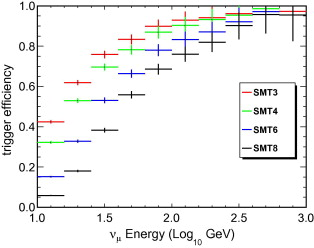
\includegraphics{figures/simulation_and_processing/trigger/trigger_efficiency.jpg}
	\caption[IceCube trigger efficiencies]{Efficiencies of different IceCube and DeepCore triggers, taken from \cite{DeepCore_design_Abbasi2012615}.}
    \labfig{trigger_efficiencies}
\end{marginfigure}

The trigger is applied inside the DOM in the ice before sending the information to the ICL on the surface. The time dependent voltage curves are captured if a pre-defined threshold value is exceeded. Once the threshold set to the equivalent of \SI{0.25}{PE} is crossed, \SI{6.4}{\micro\second} of the waveform are coarsely digitized by a \textit{Fast Analog-to-Digital Converter (FADC)} with a sampling rate of \SI{40}{\mega\hertz}. Additionally, the first \SI{427}{\nano\second} are digitized using an \textit{Analog Transient Waveform Recorder (ATWD)} with a sampling rate of \SI{300}{\mega\hertz} \sidecite{ABBASI2009294_data_acquisition}, but only if some trigger condition is met, because this readout frequency is too high to be sampled directly and requires some buffering. For DeepCore, the HLC condition already mentioned in \refsec{ice_and_DOMs} has to be met for three DOMs inside the fiducial volume within a time window of \SI{5}{\micro\second}. If this is the case, all waveforms that crossed the threshold within a \SI{20}{\micro\second} time window around the trigger are digitized and sent to the ICL for further processing. This trigger is called \textit{Simple Multiplicity Trigger 3 (SMT-3)}. The DOM hits that are read out in this process, but do not meet the HLC condition, are called \textit{soft local coincidence (SLC)} hits. The rate of the DeepCore SMT-3 trigger is $\sim$\SI{250}{\hertz} \sidecite{2017JInst..12P3012A_Instrumentation_Systems}, accepting $\sim$\SI{70}{\percent} of $\nu_\mu$-CC events at \SI{10}{\gev} and $\sim$\SI{90}{\percent} at \SI{100}{\gev} \sidecite{DeepCore_design_Abbasi2012615}. The trigger efficiencies for different SMT triggers, including the DeepCore SMT-3, are shown in \reffig{trigger_efficiencies}.


\subsubsection{Online Filter} \labsec{online_filter}

The digitized waveforms are sent to the ICL, where a further filter is applied \textit{online}\sidenote{Where \textit{online} means running on hardware at the South Pole.}. First, the WaveDeform algorithm is run to extract photon arrival times and charge from the waveforms, then the DeepCore filter is applied, which is an iterative hit cleaning starting from HLC hits and removing any hits outside a \SI{125}{\meter} radius and a \SI{500}{\nano\second} time window (called \textit{radius-time cleaning (RT-cleaning)}) of the initial hit. This mainly rejects unphysical SLC hits, which are potentially caused by random noise. The following selection steps are done using the resulting cleaned pulses.

Next, an additional cut is applied to reject events that are likely to be caused by atmospheric muons. This is done by splitting the hits depending on whether they were inside the DeepCore fiducial volume or outside and then calculating the speed of each hit outside the fiducial volume towards the \textit{center of gravity (COG)} of the hits inside. If one of them has a speed close to the speed of light, the whole event is rejected, because this is a strong indication for a muon event.

As input for the further selection levels, a few event properties, like vertex position and direction, are determined using fast and simple event reconstructions. After the DeepCore online filter, the rate is about \SI{15}{\hertz}, which can be sent to the North via satellite for further processing.


\subsection{Event Selection} \labsec{event_selection}

After the data was sent to the North, the \textit{offline} filters and selection are applied to further recude reduce the background of atmospheric muons and noise. The selection is split into three levels referred to as \textit{Level 3-5 (L3-L5)}, which bring down the neutrino and muon rate to $\sim$\SI{1}{\milli\hertz}, while the remaining fraction of random noise is below \SI{1}{\percent}.


\subsubsection{Level 3} \labsec{level_3}

At the first offline filtering level, Level 3, 1D cuts are used to reduce atmospheric muons, pure noise, and coincident muons. These cuts are targeting regions where the data/MC agreement is poor, so that more sophisticated \textit{machine learning (ML)} techniques can be applied at later levels. The cuts are made using 12 control variables, that are inexpensive to compute for the very large sample at this stage. The variables are related to position, time, and overall number of hits in the event.

Pure noise hits, that are temporally uncorrelated, are cleaned by applying a \SI{300}{\nano\second} sliding window, requiring the containment of more than 2 hits at its maximum. Additionally, an algorithm is run to check whether the hits show some directionality, accepting them only if they do.

To reduce the amount of muons a series of cuts is applied using spatial and temporal information. Events that have more than 9 hits observed above \SI{-200}{\meter} or the first HLC hit above \SI{-120}{\meter} are rejected as well as events where the fraction of hits in the first \SI{600}{\nano\second} of the event is above 0.37, ignoring the first two hit DOMs. Additionally, the ratio between hits in the veto region and the DeepCore fiducial volume is required to be below 1.5.

If a muon enters the detector after the data acquisition was already triggered, it causes events that span over a much larger time range. To reduce those coincident events, the time difference between first and last pulse cannot be above \SI{5000}{\nano\second}. This cut mainly affects a region of very poor data to MC agreement, because coincident events are not simulated at all.

The L3 cuts remove \SI{95}{\percent} of the atmospheric muons and >\SI{99}{\percent} of pure noise hits, while keeping >\SI{60}{\percent} of the neutrino events. The sample now roughly contains muons/neutrinos/noise at a ratio of 100:10:1 with a total rate of $\sim$\SI{0.5}{\hertz}.

\todo{add example plots (2?) for L3 cut variables and applied cuts}

\subsubsection{Level 4} \labsec{level_4}

After the total rate was reduced by the simple cuts of L3 and the overall agreement between data and MC is established, ML techniques can be applied to further reduce the background. For Level 4, two \textit{Boosted Decision Trees (BDTs)} \sidecite{BDT} classifier are trained to separate neutrino events from atmospheric muons and noise hits, separately. The output of each classifier, a probability score, can be seen in \reffig{level_4_classifiers}. The noise filter is applied first and an event passes the score if it is larger than 0.7, reducing the noise hits by a factor of 100, while keeping \SI{96}{\percent} of neutrinos. Then the second BDT classifier is applied to reject muons. It was trained partly on unfiltered data, which consists of >\SI{99}{\percent} atmospheric muons, to reject the data and keeping the neutrinos from the simulation. Rejecting events with a score smaller than 0.65 removes \SI{94}{\percent} of atmospheric muons while keeping \SI{87}{\percent} of neutrinos. This fraction varies depending on the flavor and interaction type, $\nu_\mu$-CC events for example, which have a muon in the final state, are therefore reduced to \SI{82.5}{\percent}. After applying the L4 cuts based on the BDT classifier outputs, the sample is still dominated by atmospheric muons, while the noise rate dropped to below most neutrino types.

\begin{figure*}
\centering 
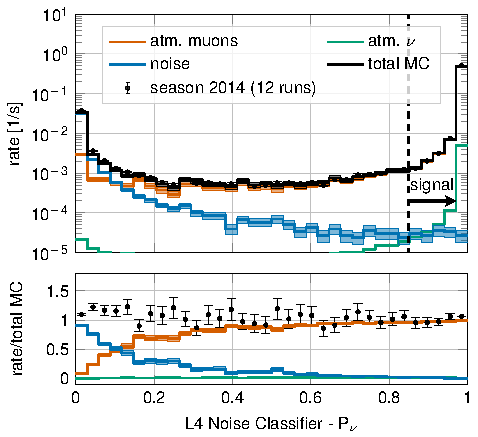
\includegraphics[width=0.49\linewidth]{figures/simulation_and_processing/selection/l4_noise_classifier_probnu.pdf}
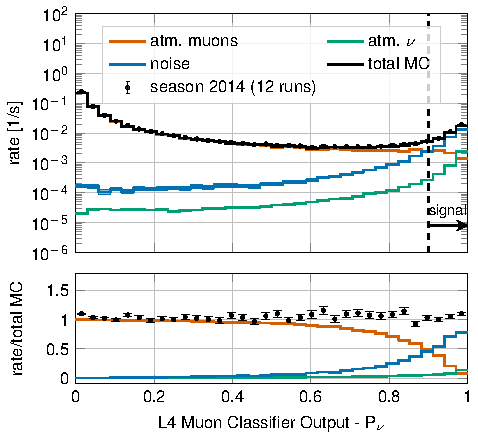
\includegraphics[width=0.49\linewidth]{figures/simulation_and_processing/selection/l4_muon_classifier_probnu.pdf}

\caption[Level 4 classifier outputs (muon and noise)]{Distributions of Level 4 noise classifier output (left) and muon classifier output (right), where larger values indicate more neutrino-like and lower values more noise-like/muon-like. Taken from \cite{OVS_PRD}.}
\labfig{level_4_classifiers}
\end{figure*}


\subsubsection{Level 5} \labsec{level_5}

Level 5 is the final selection level, before event reconstructions are applied. This level aims to reduce the remaining atmospheric muon rate below the rate of neutrinos. Muons not rejected by the earlier levels are those that produced little or no light in the veto regions. One possible reason is that they passed through one of the un-instrumented regions between the strings \todo{add some figure showing the corridors?} called \textit{corridors}. To reject those, special corridor cuts, based on the number of hits they produced close to a potential corridor they passed through. The potential corridor in questions is identified based on a simple infinite track fit. In addition to the corridor cuts, starting containment cuts are applied to reject events that start at the edge of the fiducial volume. Events with more than seven hits in the outermost strings of the detector or those that have a down going direction in the uppermost region are rejected. This further reduces the fraction of muons by \SI{96}{\percent} while keeping \SI{48}{\percent} of neutrinos. The rates after this level are \SI{1}{\milli\hertz} and \SI{2}{\milli\hertz} for neutrinos and muons, respectively, making it a neutrino dominated sample.

\todo{add table with rates per level (split in flavor) - maybe better in analysis chapter to also show signal?}


\section{Reconstruction} \labsec{reconstruction}

% Several methods exist to reconstruct events at the energies relevant for this work (\SIrange{10}{100}{\gev}).
In the energy range most relevant for this work, between \SIrange[range-phrase={~and~}]{10}{100}{\gev}, the light deposition is very low and only a few DOMs detect light, making the reconstructions difficult. In \sidecite{low_energy_reco_IC} two classical methods are described, which have partly been applied in one recent IceCube atmospheric neutrino oscillation measurement using a
% golden\sidenote{The golden sub-sample only uses events that have direct photon hits.} 
sub-sample of the DeepCore sample \sidecite{OVS_PRD}. The algorithm used in this work on the other hand, is a newer method that applies a \textit{convolutional neural network (CNN)} to reconstruct the events and determine some discriminating quantities. The latest muon neutrino disappearance result from IceCube \sidecite{flercnn_analysis_result} is based on this reconstruction.


\subsection{Fast Low Energy Reconstruction using Convolutional Neural Networks} \labsec{flercnn_reconstruction}

As the name \textit{Fast Low Energy Reconstruction using Convolutional Neural Networks (FLERCNN)} already indicates, the FLERCNN reconstruction \sidecite{flercnn_proceedings, flercnn} is a CNN optimized to reconstruct IceCube events at low energies ($<$\SI{100}{\gev}) in a fast and efficient manner, by leveraging the approximate translational invariance of event patterns within the detector.
% The network is trained to find the connection between the hit pattern and the events properties by identifying patterns similar to how CNNs are applied effectively in image classification.\todo{add references for CNN image classification?} The patterns are an imprint of the neutrino interactions that can happen anywhere in the detector, which should result in translational invariance of the events. CNNs were shown to have very good performance in identifying patterns in images, independent of their location. By combining several layers of filters of different dimensions, a map of spatial features is created from the input data and more complex features can be reconstructed.
The architecture of the network is very similar to the preexisting IceCube CNN event reconstruction \sidecite{dnn_reco_mirco}, but optimized on low energy events and specifically tailored to include the DeepCore sub-array. Only the eight DeepCore strings and the central 19 IceCube strings are used for the reconstruction (compare to \reffig{icecube_top_view}). Because of the different z-positions of the DeepCore and IceCube DOMs, they are divided into two networks that are combined in the final layer of the network. The full architecture is shown in \reffig{flercnn_network_structure}. The first dimension of the network is the string index, while the second dimension is the order of the DOMs along the vertical axis. The horizontal position of the DOMs is not used, since the strings are arranged in an irregular pattern. The information from the DOM hits is summarized into five charge and time variables, which make up the last dimension of the input layer. The variables are the total summed charge, the time of the first hit, the charge weighted mean time of the hits, the time of the last hit, and the charge weighted standard deviation of the hit times.

\todo{add image with selected strings used for flercnn IC and DC}

\begin{figure}
    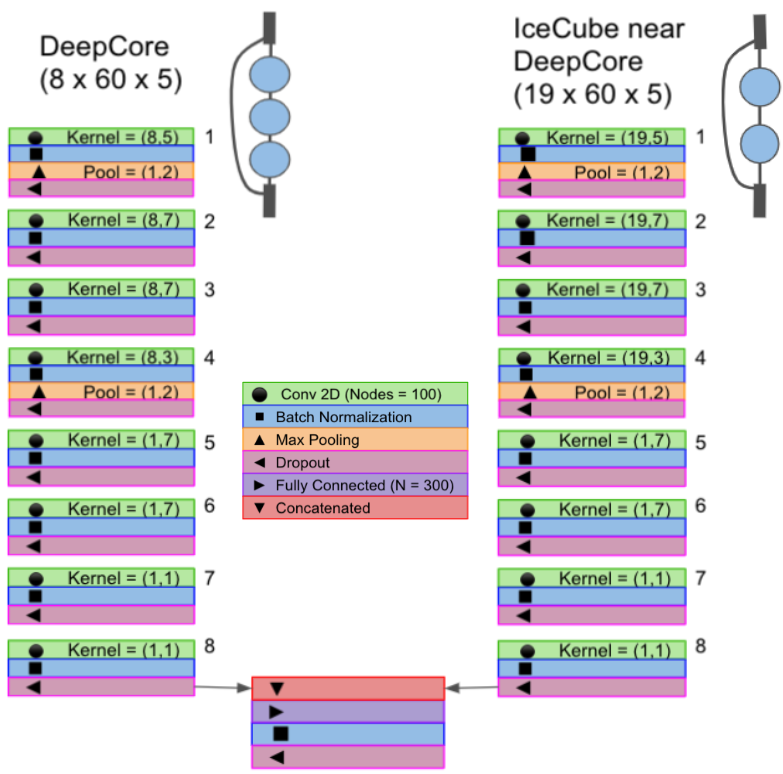
\includegraphics{figures/simulation_and_processing/flercnn/Detailed_CNN_Architecture_combined.png}
	\caption[FLERCNN architecture]{Architecture of the FLERCNN neural networks, taken from \cite{flercnn_proceedings}.}
    \labfig{flercnn_network_structure}
\end{figure}


Five different networks are trained using this architecture. Three networks do the regression of the events' energy, zenith angle, and the starting vertex ($x,y,z$ position), while two of them are used for classification. One is trained to predict the probability of the event being a track (used as PID) and the other to predict the probability of the event being a muon. Each network is trained with an MC sample modified to have a flat distribution in the target variable, to be unbiased for that variable and ideally extending outside the target reconstruction region.
% Additionally, the activation function and the loss function are adapted, according to the wanted output of the network.
For the classification tasks the loss function is the \textit{binary cross entropy} and the activation function is a \textit{sigmoid}. To perform the regression of zenith and vertex position, the loss function is the \textit{mean squared error (MSE)}, while for the energy it is the \textit{mean absolute percentage error}. The activation for all regression tasks is \textit{linear}.

\todo{add some performance plots of the FLERCNN reconstruction}

\todo{There is more information on pre-processing the samples and preparing the input features, and training each cnn, but I'm not sure if that might be too much detail?}

% \textit{INFO on resolutions:} Note that all analysis cuts are included in these resolution calculations, which results in an artificial resolution decrease near $E_{true} \approx 100$ GeV in Figure \ref{fig:EnergyResolution} due to the cut at $E_{reco} < 100$ GeV.


\subsection{Analysis Selection} \labsec{analysis_cuts}

Before the reconstruction is applied a few additional high level variables are computed, which are from fast and inexpensive algorithms. Then the reconstruction is performed by applying the trained FLERCNN networks to get the output quantities. After that, another BDT classifier is trained to further reduce the muon background for the final sample. The BDT is trained on five high level variables, where three are FLERCNN reconstruction variables (vertex $z$, $\rho_{36}$\sidenote{A radial variable that is often used in IceCube, is the horizontal distance to string 36 called $\rho_{36}$, which is basically the distance to the center of IceCube.}, and muon probability) and two are lower level variables (L4 muon classifier output and L5 corridor cut variable). To train the BDT, the FLERCNN nominal simulation set is used, only using events with $\cos(\theta_{zenith})\leq 0.3$. The output of the BDT is the neutrino probability and a cut at 0.8 is applied to reject events with a high probability of being a muon. \reffig{muon_bdt_id} shows the output of the BDT classifier, where the neutrinos in both training and testing sets are gathered at 1 and muons are around 0, which shows great classification power.

\begin{figure*}
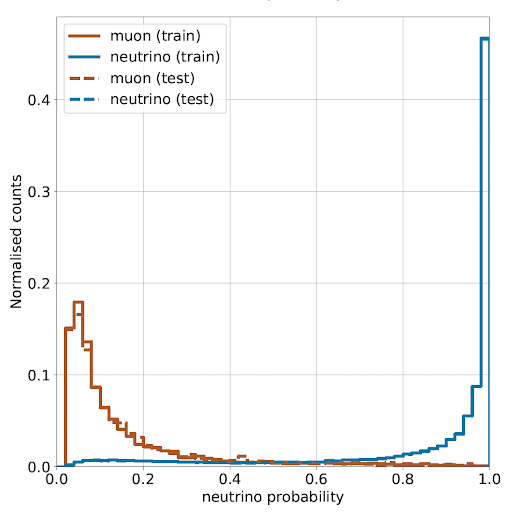
\includegraphics[width=0.49\linewidth]{figures/simulation_and_processing/flercnn/flercnn_muon_classifier.png}
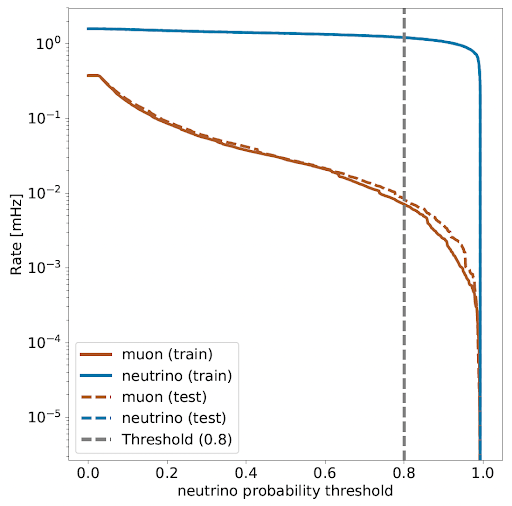
\includegraphics[width=0.49\linewidth]{figures/simulation_and_processing/flercnn/flercnn_muon_classifier_rate_vs_threshold.png}
\caption[FLERCNN muon classifier probability distributions]{FLERCNN muon classifier output score (left) and rate of neutrinos and muons as function of muon classifier cut (right). Taken from \cite{flercnn_analysis_internal_note}}
\labfig{muon_bdt_id}
\end{figure*}

\todo{add reference for flercnn analysis internal note}

To get the final, pure sample of well reconstructed neutrinos another set of cuts is applied. The first cuts are meant to reject events with poor reconstruction quality, by requiring the events to fall into the DeepCore volume, where the denser, better instrumented detector leads to enhanced resolution. The cuts are applied on the vertex $z$ and $\rho_{36}$ and are listed in \reftab{analysis_cuts}. The FLERCNN reconstruction was optimized for atmospheric neutrino analyses which are mainly in the region below \SI{100}{\gev} and there are very few events with energies below \SI{5}{\gev}, so the reconstructed energy is required to be in that range. Additionally, rejecting events with fewer than seven hits in the selected DOMs used for FLERCNN showed to increase the resolution.

Another set of cuts is applied to make sure the agreement between data and MC is good. To remove coincident muon and neutrino events, cuts are applied to the number of hits in the top 15 layers of IceCube DOMs and the number of hits in the outermost IceCube strings. Coincident random noise events are removed by requiring more than three hit DOMs from direct photons\sidenote{\textit{Direct photons} are photons that were not scattered on their way from the interaction vertex to the DOM.}. Neither of the two coincident event types are simulated, which can be seen as bad agreement between data and MC. The last cut is on the reconstructed cosine zenith, which is required to be smaller than 0.04 to reject down-going muons.

\begin{table}
    \small
        % \begin{tabular}{ p{0.36\textwidth} p{0.26\textwidth} p{0.25\textwidth} }
        \begin{tabular}{ lll }
        \hline\hline
    
        \textbf{Variable} & \textbf{Threshold} & \textbf{Removed} \\ 
    
        \hline\hline
    
        Number of hit DOMs & $\geq 7$ & \SI{1.05}{\percent} \\
        Radial distance & < \SI{200}{\meter} & \SI{0.09}{\percent} \\
        Vertical position & \SI{-495}{\meter} < z < \SI{-225}{\meter} & \SI{5.48}{\percent} \\
        Energy & \SI{5}{\gev} < E < \SI{100}{\gev} & \SI{20.70}{\percent} \\
    
        Cosine of zenith angle & < 0.04 & \SI{19.66}{\percent} \\
        Number of direct hits & > 2.5 & \SI{10.50}{\percent} \\
        Number of hits in top layers & < 0.5 & \SI{0.03}{\percent} \\
        Number of hits in outer layer & < 7.5 & \SI{0.001}{\percent} \\
        Muon classifier score & $\geq 0.8$ & \SI{23.90}{\percent} \\

        \hline
        \end{tabular}
    \caption[Final analysis cuts]{Cuts performed to select the final analysis sample. Parts of the cuts are meant to increase the data/MC agreement, while others are meant to reject events with poor reconstruction quality.}
    \labtab{analysis_cuts}
    \end{table}
    

\todo{add final sample composition, but maybe also in analysis chapter to show signal and background?}

\todo{at some place I will want a selection efficiency plot for SM BG and HNL signal, but I'm not sure where to put it yet}


\section{Systematic Uncertainties} \labsec{systematic_uncertainties}

There are multiple sources of systematic uncertainties related to the event generation and processing explained in this chapter. 
% Since variations in the range of these uncertainties change the expected number of events in the analysis, it is important to estimate their impact on the final results.
All uncertainties considered in this work are implemented with parameters that can be varied continuously so that a simultaneous fit of the physics and systematic parameters can be performed. Where possible, a correct model of the effect is used, but in many cases the variations are captured by effective parameters. Uncertainties that solely scale the total event rate are not included individually, since the analysis only uses the relative distribution of events. A single scaling parameter $A_\rm{eff}$ is used to scale the total neutrino rate instead.


\subsection{Atmospheric Flux Uncertainties}

The flux of atmospheric neutrinos is influenced by multiple factors, the spectrum and composition of CRs, the assumed atmospheric conditions, and the HI model used to describe the air showers development. Uncertainties of the neutrino flux are therefore dictated by the uncertainties on these components, where the variations in atmospheric conditions were found to have negligible effect \sidecite{OVS_PRD}.


\paragraph{Cosmic ray flux:}

The selected sample of atmospheric neutrinos lies around energies of up to \SI{100}{\gev}. The initial primary particles in the CR flux can have 100 times larger energies and therefore the CR flux between \SI{10}{\gev} and \SI{10}{\tera\electronvolt} is important, which dominantly consists of hydrogen and helium nuclei \sidecite{cosmic_ray_composition_and_GSF}. The uncertainty in this CR flux component can be described as a power law correction \sidecite{PhysRevD.74.094009, PhysRevD.95.023012}
\begin{equation}
    \Phi^\prime_\nu = \Phi_\nu \left( \frac{E}{E^\star} \right)^{\Delta\gamma}
    \;,
    \labeq{power_law_flux_uncertainty}
\end{equation}
where $E^\star$ is the pivot energy and $\Delta\gamma$ is the correction to the power law exponent. This modification propagates into the neutrino flux, which is therefore corrected in the same way. $E^\star$ was chosen to be \SI{24}{\gev} as to minimize the dependence of the overall flux scale on $\Delta\gamma$ \sidecite{OVS_PRD}.


\paragraph{Hadronic interaction model:}

Neutrinos are produced in the decaying hadrons in CR air showers, spanning a large parameter space that is sparsely evaluated by experimental data. To include uncertainties based on energy, direction, and neutrino flavor, the \textsc{MCEq} package \cite{mceq} is used to compute the distribution of atmospheric leptons and to estimate the impact of varying their contributions. The calculations result in the change in flux $d\Phi_\rm{l}/dB$ for a variation $dB$ of some parameter $B$. Scaling this variation by some value $b$, the modified total flux, s is then given by
\begin{equation}
    \Phi^\prime_\rm{l} = \Phi_\rm{l} + \left( b \cdot \frac{d\Phi_\rm{l}}{dB} \right)
    \;.
    \labeq{mceq_flux_variations}
\end{equation}
Matching the work in \sidecite{Barr:2006it}, the parameter space is divided in regions of the primary energy $E_i$ and the energy fraction of the secondary meson $x_\rm{lab}$, with varying uncertainties, derived from fixed target experiment data\todo{add figure with Barr blocks?}. The Sibyll2.3c \sidecite{sibyll2.3d} HI model and the GSF CR flux \sidecite{cosmic_ray_composition_and_GSF} were used to calculate the related flux changes\sidenote{The choice of flux and HI model have minor impact on the variations.} for the different regions in $E_i$ and $x_\rm{lab}$, resulting in 17 variables, encoding the possible changes.


\subsection{Cross-Section Uncertainties}

The uncertainties related to the cross-sections are split into low and high energy components, since there is no coherent model to explain both DIS interactions, which are the dominant processes above \SI{20}{\gev}, and \textit{charged current resonance production (CCRES)} and \textit{charged current quasi elastic scattering {CCQE}}, which are relevant below \SI{20}{\gev} where interactions with the nucleons as a whole are important. Three parameters are included to account for all relevant cross-sections uncertainties.

At low energies two parameters are included accounting for uncertainties in form factors of CCQE and CCRES events. These uncertainties are due to uncertainties in the \textit{axial mass} $M_\rm{A}$, which enters the form factor as in
\begin{equation}
    F(Q^2) \sim \frac{1}{(1 - (\frac{Q}{M_\rm{A}})^2)^2}
    \;,
\end{equation}
where $Q^2$ is the momentum transfer squared. The axial mass can be determined experimentally\todo{which experiments measure the axial mass?} and to include uncertainties on the values of $M_\rm{A}^\rm{CCQE}$ and $M_\rm{A}^\rm{CCRES}$, the cross-sections are computed with GENIE, where the form factors are calculated varying the axial mass by $\pm 20\% (1\sigma)$/$\pm 40\% (1\sigma)$ around the nominal value. This is an approximation of the recommended uncertainties by the GENIE collaboration, which are $-15\%$, $+25\%$ for $M_\rm{A}^\rm{CCQE}$ and $\pm 20\%$ for $M_\rm{A}^\rm{CCRES}$ \cite{genie}. To apply a continuous uncertainty variation of the axial mass in a fit, the total cross-section is fit with a quadratic function to interpolate between the cross-sections computed with the different axial masses.

Even though the DIS interactions can be calculated very precisely, there are still uncertainties in the input PDF, describing the probability of finding a specific parton (quark) with a specific momentum fraction $x$ inside a nucleon. To account for differences between the used method and more sophisticated methods using newer PDFs seen at high energies, an uncertainty parameter is introduced. The parameter is based on the discrepancy between the cross-sections computed with GENIE and the ones computed with CSMS \sidecite{csms} above \SI{100}{\gev}. The included parameter scales the cross-section from the GENIE values to the CSMS values, which are considered more accurate above \SI{100}{\gev}. The scaling is done as a function of energy and inelasticity and to guarantee continuity, the scaling is extrapolated linearly below \SI{100}{\gev}. The parameter is designed such that a value of 0.0 corresponds to the GENIE cross-sections and a value of 1.0 gives an approximation of the CSMS cross-sections. A comparison of the total cross-sections GENIE (scaled/unscaled) with the data is shown in \reffig{dis_systematic_effect}.

\begin{figure*}
    \centering 
    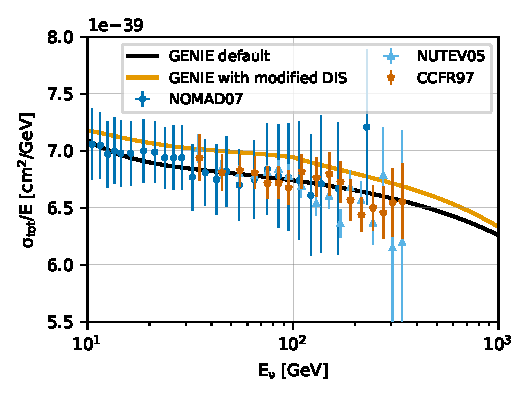
\includegraphics[width=0.49\linewidth]{figures/simulation_and_processing/cross_sections/NuMu_CC_iso_comp_to_data__upd_style.pdf}
    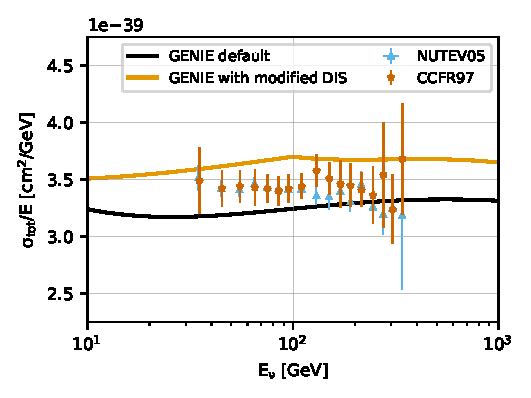
\includegraphics[width=0.49\linewidth]{figures/simulation_and_processing/cross_sections/NuMu_Bar_CC_iso_comp_to_data__upd_style.pdf}
    
    \caption[Inclusive total neutrino-nucleon cross-sections]{Inclusive total neutrino-nucleon cross-sections on an isoscalar target (black) for neutrinos (left) and antineutrinos (right) calculated with GENIE, comparing to measurements from NOMAD \cite{xsec_data_nomad}, NUTEV \cite{xsec_data_nutev}, and CCFR \cite{xsec_data_ccfr}. The scaled GENIE cross-section (orange) is also shown. Taken from \cite{OVS_PRD}.}
    \labfig{dis_systematic_effect}
\end{figure*}


\subsection{Detector Calibration Uncertainties}

There are multiple sources of systematic uncertainties related to the detection process of neutrinos in IceCube. Dominant for this analysis are the effects of the properties of the ice itself and the optical efficiency of the DOMs. None of these uncertainties can be described by an analytic expression, so they have to be estimated using MC simulation. The method used to derive the continuous variations based on the MC simulation is described in \refsec{ultrasurfaces}. The five relevant uncertainty parameters are the absolute efficiency of the DOMs, a global scaling of bulk ice scattering and absorption lengths, and variations of the relative angular acceptance due to hole ice variations in two parameters.


\paragraph{DOM efficiency:}
As was already mentioned in \refsec{ice_and_DOMs}, the absolute efficiency of the DOMs, $\epsilon_\rm{DOM}$ is calibrated using minimum ionizing muons from air showers, due to the lack of a calibrated light source in the detector. Using the muons as a steady, controlled source of light, the efficiency can be estimated by comparing simulated muon data sets with varied DOM response to the measured data. Since the uncertainties found in multiple iterations of this study \sidecite{JFeintzeig_phd, domeff_nick} are at the order of \SI{10}{\percent}, this systematic is highly relevant and has to be included in the analysis.


\paragraph{Bulk ice scattering and absorption:}

Absorption and scattering length are the most important properties that govern the propagation of photons through the ice. The simulation principle and how the depth dependent absorption and scattering coefficients are used was already explained in \refsec{photon_propagation}. To account for uncertainties on this model of the bulk ice coefficients, a global scaling for each of the two parameters (global absoprtion, global scatteriong) is applied.


\paragraph{Hole ice angular acceptance:}

Due to bubble formation in the re-freezing process of the boreholes, the hole ice seems to be less transparent in the center of the columns \sidecite{rongen_drilling_epj}. This effectively decreases the chance of photons hitting the DOMs directly from below, which can be described as an additional angular modification of the DOM acceptance. The modification is parameterized by a two dimensional, normalized\sidenote{The hole ice angular acceptance modification is normalized so that it does not affect the total charge.} function, where the two dominant of the parameters ($p_0, p_1$), dictating its form, are enough to describe all past and the current hole ice models from both \textit{in-situ} and laboratory measurements. \reffig{hole_ice_variations} shows the acceptance modification as a function of the incident photon angle $\cos(\eta)$. The current baseline model, the variations achieved through modifying $p_0$ and $p_1$, and a laboratory measurement can be seen.

\begin{figure}
    \centering
    \begin{tikzpicture}

\pgfplotstableread{figures/simulation_and_processing/hole_ice/angsens_example_fluct.csv}\table
\pgfplotstableread[col sep=comma]{figures/simulation_and_processing/hole_ice/all_acceptance_curves.csv}\acceptancecurves

    \begin{axis}[
            xmajorgrids, ymajorgrids,
            xlabel=$\cos(\eta)$, ylabel=relative optical efficiency,
            legend style={at={(0.02,0.95)}, anchor=north west},
            ytick distance=0.2,
        ]

        \addplot[black, thick] table [x=cos_theta, y=baseline] \acceptancecurves;
        \addlegendentry{baseline}
        
        \addplot[vermilion, thick] table [x=cos_theta, y=nominal] \acceptancecurves;
        \addlegendentry{laboratory}
        
        \addplot[tab_blue, thin, name path=fluct_p0_dn, forget plot] table [x=cos_theta, y=fluct_p0_dn] \table;
        \addplot[tab_blue, thin, name path=fluct_p0_up, forget plot] table [x=cos_theta, y=fluct_p0_up] \table;
        \addplot[tab_blue, opacity=0.5] fill between[of = fluct_p0_dn and fluct_p0_up];
        \addlegendentry{example variation in $p_0$}
        
        \addplot[tab_orange, thin, name path=fluct_p1_dn, forget plot] table [x=cos_theta, y=fluct_p1_dn] \table;
        \addplot[tab_orange, thin, name path=fluct_p1_up, forget plot] table [x=cos_theta, y=fluct_p1_up] \table;
        \addplot[tab_orange, opacity=0.5] fill between[of = fluct_p1_dn and fluct_p1_up];
        \addlegendentry{example variation in $p_1$}
	
    \end{axis}
\end{tikzpicture}

    \caption[Hole ice angular acceptance modification]{Relative angular acceptance modification due to hole ice. Shown is the current baseline model, the variations from changing $p_0$ and $p_1$, and a laboratory measurement. Modified from \cite{ATrettin_phd}.}
    \labfig{hole_ice_variations}
\end{figure}


\subsection{Muon Uncertainties}

The muon fraction in the final level selection (see \refsec{analysis_cuts}) is below \SI{1}{\percent}, therefore additional muon systematic uncertainties apart from the spectral index are not implemented, but rather a total muon scaling parameter is added. This total scale is somewhat degenerate with the DOM efficiency, since an increased DOM efficiency leads to better muon rejection\todo{cite this?}. Both the total muon scaling and the muon spectral index have a very small impact on the analysis as will be shown in \refsec{parameter_selection}.


% \setchapterstyle{kao}
\setchapterpreamble[u]{\margintoc}

\chapter{Detecting Low Energetic Double Cascades}
\labch{double_cascade_performance}


\section{Reconstruction}

\subsection{Table-Based Minimum Likelihood Algorithms}

\subsection{Double Cascade Hypothesis}

\subsection{Modification to Low Energy Events}

\section{Cross Checks}
\subsection{Simplistic Sets}

After generation the events are processed with standard Photon, Detector, L1, and L2 processing and then Taupede+MuMillipede is run on top of the L2 files. Multiple versions with different parameters were produced, some with the OscNext baseline parameters, some without detector noise (in Det level) and some with h2-50cm holeice model, to match the holeice model that was used to generate the photonics tables.


\paragraph{BrightDom Cleaning}

To investigate the effect of the BrightDom cleaning cut the 194601 set without detector noise (and baseline hole ice model) is used. The BrightDom cleaning is needed to stop a few DOMs with many photon hits to drive the reconstruction because this leads to large biases in the energy estimations. Historically, the BrightDom cleaning was removing all DOMs that had a charge larger than 10 times the mean charge. After quickly checking some charge distributions and how the mean behaves it was clear that the cut should better be defined based on a metric that is less affected by outliers, like the median. \reffig{bright_dom_cleaning_charges_mean_median} shows where the mean and the median are located for an example event. The cut was re-defined to use the median instead of the mean and 10\% of the simulation were processed with \href{https://github.com/LeanderFischer/I3_HNL_Decay/blob/a6838ec48e0a2d4f6547cbe064d2928ec55fb76d/submission_scripts/process/process_Taupede.py}{Taupede} using 30x and 100x the median as BrightDom cutoff. \reffig{bright_dom_cleaning_charges_median_scales} shows where these values fall for the same example event.

% \begin{figure}[h!]
%     \subfloat[\labfig{bright_dom_cleaning_charges_mean_median}]{
%         \includegraphics[width=.45\linewidth]{figures/upgoing_string_81_gen_level/brightdom_cleaning/median_and_mean_L2_00001.i3.zst_SplitInIcePulses_frame_0.png}
%         }
%     \subfloat[\labfig{bright_dom_cleaning_charges_median_scales}]{
%         \includegraphics[width=.45\linewidth]{figures/upgoing_string_81_gen_level/brightdom_cleaning/median_scales_L2_00001.i3.zst_SplitInIcePulses_frame_0.png}
%         }
%     \caption{Charge distribution of example event showing mean and median charge (left) and different scales of median charge (right).}
%     \labfig{bright_dom_cleaning_charges}
% \end{figure}

As a quick check of the performance of both cuts the decay length resolution/bias and the resolutions/biases of all energies were checked. The reconstructed decay length is almost not affected by applying this cut, which is as expected, because it is mostly dependent on the arrival time of the photons. The effect on the reconstructed energy is much stronger, where a looser cut (100x) shows a significantly larger bias than the tighter cut at (30x). Even though this was not a highly sophisticated optimization of the BrightDom cut, an improvement was achieved by changing from mean to median and selecting the tighter cut (of the two tested). It's hard to tell how this would perform for high energy events, but I'm quite certain that a definition based on the median would be more reliable than on the mean.

% \begin{figure}[h!]
%     \subfloat[\labfig{bright_dom_cleaning_performance_decay_length_bias}]{
%         \includegraphics[width=.45\linewidth]{figures/upgoing_string_81_gen_level/brightdom_cleaning/median_decay_length_bias_fullset_larger_range_unweighted.png}
%         }
%     \subfloat[\labfig{bright_dom_cleaning_performance_total_energy_bias}]{
%         \includegraphics[width=.45\linewidth]{figures/upgoing_string_81_gen_level/brightdom_cleaning/compare_bright_dom_cuts_fractional_reco_total_energy_error_fully.png}
%         }
%     \caption{Decay length bias (left) and total energy bias (right).}
%     \labfig{bright_dom_cleaning_performance}
% \end{figure}

\section{Performance}

\subsection{Energy/Decay Length Resolution}

\subsection{Double Cascade Classification}


% \setchapterstyle{kao}
\setchapterpreamble[u]{\margintoc}

\chapter{Search for Tau Neutrino Induced Heavy Neutral Lepton Events}
% \chapter{Search for tau neutrinoo-induced Heavy Neutral Lepton Events}
\labch{analysis}

This chapter describes the search for HNL events\todo{make sure I don't use the phrasing "search for an excess of HNL events" anywhere.. (ORANGE)} using \SI{10}{years} of IceCube DeepCore data. The expected number of HNL events in the data sample depends on the mass of the additional heavy state, $m_4$, and the mixing element $|U_{\alpha4}^2|$, with $\alpha=e,\mu,\tau$, between the SM flavors and the new mass state. As discussed in \refsec{HNL_model_to_be_tested}, this work focuses on the mixing to the tau sector, $|U_{\tau4}^2|$, which has the weakest constraints to date.
% In principle the two physics parameters to be probed are the mass of the HNL, $m_4$, and the mixing between the fourth heavy mass state and the SM $\tau$ sector, $|U_{\tau4}|^2$.
Since the mass itself influences the production and decay kinematics of the event and the accessible decay modes, individual mass samples were produced as described in \refsec{model_specific_simulation}. The mass influences the energy distribution, while the mixing both changes the overall scale of the HNL events and the shape in energy and PID.
% IceCube DeepCore is suited to measure the excess which appears around and below \SI{20}{\gev}, due to its production from the atmospheric tau neutrinos, although a reduced lower energy threshold might improve the analysis.
The search is performed for the three mass samples individually, while the mixing is the parameter that can be varied continuously and is measured in the fit.


\section{Final Level Sample} \labsec{analysis_samples}

The final level sample of this analysis consists of the neutrino and muon MC introduced in \refsec{sm_event_generation} and one of the three HNL samples explained in \refsec{model_specific_simulation}. All simulation and the \SI{10}{years} of IceCube DeepCore data are processed through the full processing and event selection chain described in \refsec{processing_chain} and \refsec{reconstruction} leading to the final level sample. As described in \refsec{analysis_cuts}, event triggers consisting purely of random coincidences induced by noise in the DOMs have been reduced to a negligible rate, and will not be discussed further.

\todo{add information about the matter profile used (ORANGE)}
\todo{add information about the oscillation probability calculation and the software used for it (RED)}

\subsection{Expected Rates/Events}

The rates and the expected number of events for the SM background are shown in \reftab{background_final_level_expectation} with around 175000 total events expected in the \SI{10}{years}. The explicit, good detector livetime in this data taking period is \SI{9.28}{years}. The rates are calculated by summing the weights of all events in the final level sample, while the uncertainties are calculated by taking the square root of the sum of the weights squared. The expected number of events is calculated by multiplying the rate with the livetime. The individual fractions show that this sample is neutrino dominated where the majority of events are $\nu_\mu$-CC events.

\begin{table}[h]
    \begin{tabular}{ lccc }
    \hline\hline
    \textbf{Type} & \textbf{Rate [\si{\milli\hertz}]} & \textbf{Events (in \SI{9.28}{years})} & \textbf{Fraction [\si{\percent}]} \\ 
    \hline\hline
    $\nu_\mu^\rm{CC}$   & 0.3531 & 103321 $\pm$ 113 & 58.9 \\
    $\nu_e^\rm{CC}$     & 0.1418 & 41490 $\pm$ 69 & 23.7 \\
    $\nu_\rm{NC}$       & 0.0666 & 19491 $\pm$ 47 & 11.1 \\
    $\nu_\tau^\rm{CC}$  & 0.0345 & 10094 $\pm$ 22 & 5.8 \\
    $\mu$               & 0.0032 & 936 $\pm$ 15 & 0.5 \\
    \hline
    total               & 0.5991 & 175336 $\pm$ 143 & 100.0  \\
    \hline
    \end{tabular}
\caption[Final level background event/rate expectation]{Final level rates and event expectation of the SM background particle types.}
\labtab{background_final_level_expectation}
\end{table}

\todo{Should I adapt the total numbers to match the sum of the rounded individual parts? (YELLOW)}

\reftab{signal_final_level_expectation} shows the rates and expected number of events for the HNL signal simulation. The expectation depends on the mass and the mixing and shown here are two example mixings for all the three masses that are being tested in this work. A mixing of $0.0$ would result in no HNL events at all. It can already be seen that for the smaller mixing of $|U_{\tau4}|^2=10^{-3}$ the expected number of events is very low, while at the larger mixing of $|U_{\tau4}|^2=10^{-1}$ the number is comparable to the amount of muons in the background sample. 

\begin{table}[h]
    \begin{tabular}{ lcc }
    \hline\hline

    \textbf{HNL mass} & \textbf{Rate [\si{\micro\hertz}]} & \textbf{Events (in \SI{9.28}{years})} \\

    \hline\hline
    \textbf{$|U_{\tau4}|^2=10^{-1}$} & & \\ 
    \hline
    \SI{0.3}{\gev} & 3.3298 $\pm$ 0.0053 & 974.5 $\pm$ 1.6 \\
    \SI{0.6}{\gev} & 3.0583 $\pm$ 0.0058 & 895.0 $\pm$ 1.7 \\
    \SI{1.0}{\gev} & 2.4988 $\pm$ 0.0059 & 731.3 $\pm$ 1.7 \\
    \hline
    \textbf{$|U_{\tau4}|^2=10^{-3}$} & & \\ 
    \hline
    \SI{0.3}{\gev} & 0.0057 & 1.67 $\pm$ 0.01 \\
    \SI{0.6}{\gev} & 0.0220 & 6.44 $\pm$ 0.01 \\
    \SI{1.0}{\gev} & 0.0248 & 7.27 $\pm$ 0.01 \\
    % \SI{0.3}{\gev} & 0.00571 $\pm$ 0.00002 & 1.67 $\pm$ 0.01 \\
    % \SI{0.6}{\gev} & 0.02200 $\pm$ 0.00004 & 6.44 $\pm$ 0.01 \\
    % \SI{1.0}{\gev} & 0.02484 $\pm$ 0.00005 & 7.27 $\pm$ 0.01 \\
    \hline
    \end{tabular}
\caption[Final level signal event/rate expectation]{Final level rates and event expectations of the HNL signal for all three masses and two example mixing values.}
\labtab{signal_final_level_expectation}
\end{table}


\subsection{Analysis Binning}

\begin{figure*}[h]
    \includegraphics[trim=7cm 0cm 12cm 1cm, clip]{figures/results/labeled_s_to_sqrt_b_1.0_GeV_combined_U_tau4_sq_0.1000_total.png}
    \caption[]{}
    \labfig{s_to_sqrt_b_1.0_GeV_0.1_mixing}
\end{figure*}
\todo{fix caption (RED)}

An identical binning to the analysis performed in \sidecite{flercnn_analysis_result} is used. In total, there are three bins in PID (cascade-like, mixed, and track-like), 12 bins in reconstructed energy, and 8 bins in cosine of the reconstructed zenith angle as specified in \reftab{analysis_binning}.
% It was chosen such that the track-like bin has the largest $\nu_\mu$-CC fraction and a bin with a mixture of track and cascade events exists.
Extending the binning towards lower energies or increasing the number of bins in energy or cosine of the zenith angle did not improve the HNL sensitivities significantly, because the dominant signal region is already covered with a sufficiently fine binning to observe the shape and magnitude of the HNL events. This can be seen in the middle panel of \reffig{s_to_sqrt_b_1.0_GeV_0.1_mixing}. To ensure that sufficient data events end up in the individual bins to result in a good fit, a few bins were not taken into account in the analysis that showed low data statistics. Those are shown in dark green in the 3-d histogram.
% Originally, there were two more bins in $\cos(\theta)$, which were removed to reduce muons coming from the horizon and some low energy bins in the cascade-like bin are removed due to the low event statistics.

\begin{table}[h]
        \begin{tabular}{ llll }
        \hline\hline    
        \textbf{Variable} & \textbf{$N_\rm{bins}$} & \textbf{Edges} & \textbf{Step} \\     
        \hline\hline    
        $P_\nu$ & 3 & [0.00, 0.25, 0.55, 1.00] & linear \\
        $E$ & 12 & [5.00, 100.00] & logarithmic \\
        $\cos(\theta)$ & 8 & [-1.00, 0.04] & linear \\    
        \hline
        \end{tabular}
    \caption[Analysis binning]{Three dimensional binning used in the analysis. All variables are from the FLERCNN reconstruction explained in \refsec{reconstruction}.}
    \labtab{analysis_binning}
\end{table}

\todo{add 3D data histograms (RED)}
\todo{Add fractions of the different particle types in the bins for benchmark mass/mixing (another table?) (ORANGE)}


\section{Statistical Analysis} \labsec{analysis_principle}

\subsection{Test Statistic}

\todo{I feel like I have to be a bit more precise on what is the fit metric (e.g. the mod chi2) and what is the TS, as in the mod chi2 difference, which is the actual TS, right? (RED)}

The measurements are performed by comparing the weighted MC to the data. Through variation of the nuisance and physics parameters that govern the weights, the best matching set of parameters can be found. The comparison is done using a modified $\chi^2$ defined as
\begin{equation}
    \chi^2_{\mathrm{mod}} = 
    \sum_{i \in \mathrm{bins}}^{}\frac{(N^{\rm{exp}}_i - N^{\mathrm{obs}}_i)^2}
    {N^{\rm{exp}}_i + (\sigma^{\mathrm{\nu}}_i)^2 + (\sigma^{\mathrm{\mu}}_i)^2 + (\sigma^{\mathrm{HNL}}_i)^2}
     + \sum_{j \in \mathrm{syst}}^{}\frac{(s_j - \hat{s_j})^2}{\sigma^2_{s_j}}
    \;,
    \labeq{mod-chi2-hnl}
\end{equation}
as the \textit{test statistic (TS)}. The total even expectation is $N^{\rm{exp}}_i = N^{\mathrm{\nu}}_i + N^{\mathrm{\mu}}_i + N^{\mathrm{HNL}}_i$, where $N^{\mathrm{\nu}}_i$, $N^{\mathrm{\mu}}_i$, and $N^{\mathrm{HNL}}_i$ are the expected number of events in bin $i$ from neutrinos, atmospheric muons, and HNLs, while $N^{\mathrm{obs}}_i$ is the observed number of events in bin $i$. The expected number of events from each particle type is calculated by summing the weights of all events in the bin $N^{\mathrm{type}}_i = \sum_i^\rm{type}\omega_i$, with the statistical uncertainty being $(\sigma^{\mathrm{type}}_i)^2 = \sum_i^\rm{type}\omega_i^2$. The additional term in \refeq{mod-chi2-hnl} is included to apply a penalty term for prior knowledge of the systematic uncertainties of the parameters where they are known. $s_j$ are the systematic parameters that are varied in the fit, while $\hat{s_j}$ are their nominal values and $\sigma_{s_j}$ are the known uncertainties.

\todo{Do I want/need to include the description of the KDE muon estimation? (YELLOW)}


\subsection{Physics Parameters} \labsec{analysis_parameters}

The variable physics parameter in this analysis is the mixing between the HNL and the SM $\tau$ sector, $|U_{\tau4}|^2$. It can be changed continuously in the range of [\SI{0.0}, \SI{1.0}] by applying the weighting scheme described in \refsec{hnl_weighting_scheme}. The fit is initialized at an off-nominal value of \SI{0.1}. The other physics parameter, the mass $m_4$ of the HNL, is fixed to one of the three discrete masses to be tested, by using the corresponding sample of the HNL simulation described in \refsec{model_specific_simulation}.


\subsection{Nuisance Parameters} \labsec{analysis_systematics}

\begin{marginfigure}
    \includegraphics{figures/results/checks/plot_systematic_impact_ranking.png}
	\caption[xx]{"calculated at a mixing of 0.1 and for the 1.0 GeV sample"}
    \labfig{systematic_impact_test}
\end{marginfigure}
\todo{Blow up labels/legend/title and make it more readable in the margin or move it into the main text? (RED)}
To decide which systematic uncertainties should be included in the fit, we test the potential impact they have on the TS if they are neglected. The test is performed by creating Asimov data using the BG simulation and the HNL simulation of the \SI{1.0}{\gev} mass sample at a mixing value of $0.1$, which is chosen as a benchmark physics parameter and does not have a significant impact on the test. The systematic parameter of interest is set to a value above its nominal expectation, either pulled up by $+1\sigma$ or by an educated estimate for parameters without a well-defined uncertainty. A fit is performed fixing the systematic parameter of interest and leaving all additional parameters free. The resulting TS is the mis-modeling significance between this fit and a fit with all parameters free, which would result in a TS of 0.0 for this Asimov test\todo{I don't like this formulation, but don't know better right now.. (YELLOW)}. Parameters below a significance of \SI{0.1}{\sigma} are fixed, and the test is performed in an iterative manner until the final set of free parameters is found. \reffig{systematic_impact_test} shows the resulting significances of one of these tests. In the final selection of free parameters the Barr $h_{\pi^+}$ parameter was also left free\todo{elaborate why this is also done to cover the whole energy range for the Pion production, referencing the Barr Block plot that I haven't included yet :D (RED)} and the ice absorption is still kept free, despite showing a small significance. This is done because the bulk ice parameters are not well constrained and are known to have a large impact, which might be concealed in the test, due to correlations with the other parameters\todo{I truly dislike this sentence, too, better ideas? (YELLOW)}.

\todo{I'm just writing out the data from the table, but I need to mention/motivate the included priors here and maybe just point to the table for the ranges/nominal values? (Not quite sure about this) (RED)}The scaling parameter $N_{\nu}$ is included to account for the unknown overall normalization of the neutrino rate. It has the identical effect on the SM neutrino events and the BSM HNL events and its nominal value is set to 1.0 with a wide range of [$0.1$, $2.0$].

Concerning the atmospheric neutrino flux, the CR power law flux correction factor $\Delta \gamma_\nu$ is included with nominal value of 0.0 and a range of [$-0.5$, $0.5$]. The nominal value corresponds to a CR power law of $E^{-2}$ and a slightly conservative prior of 0.1 is applied to the parameter, while latest measurements have an uncertainty of 0.05 \sidecite{PhysRevD.95.023012}.

Additionally, the Barr $h_{\pi^+}$, Barr $i_{\pi^+}$, and Barr $y_{K^+}$ parameters of the Pion and Kaon production uncertainties are included with nominal values of $0.0$ and ranges of [$-0.75$, $0.75$], [$-3.05$, $3.05$], and [$-1.5$, $1.5$], respectively.\todo{say something about their priors (RED)}

From the cross-section uncertainties introduced in \refsec{cross_section_uncertainties}, all three parameters, $\rm{DIS}$, $M_\rm{A,QE}$, and $M_\rm{A,res}$ are included in the fit with nominal values of $0.0$ for all of them and range [$-0.5$, $1.5$] for $\rm{DIS}$ and [$-2.0$, $2.0$] for the axial mass parameters $M_\rm{A,QE}$, and $M_\rm{A,res}$.\todo{say something about their priors (RED)}

All the detector systematic uncertainties are included in the fit. The DOM efficiency $\epsilon_{\rm{DOM}}$ has a nominal value of $1.0$ and a range of [$0.8$, $1.2$]. It is constrained by a Gaussian prior with a width of $0.1$, which is a conservative estimate based on the studies of the optical efficiency using minimum ionizing muons from \sidecite{JFeintzeig_phd, domeff_nick}. The hole ice model parameters $p_0$ and $p_1$ are included with nominal values of $0.101569$ and $-0.049344$, respectively, and ranges of [$-0.6$, $0.5$] and [$-0.2$, $0.2$]. The bulk ice absorption and scattering parameters are included with nominal values of $1.0$ and $1.05$, respectively, and ranges of [$0.85$, $1.15$] and [$0.9$, $1.2$]. They are unconstrained in the fit and the ranges are set to be conservative determined from calibration data\todo{cite?! (ORANGE)}

The two atmospheric neutrino oscillation parameters $\theta_{23}$ and $\Delta m^{2}_{31}$ are also included in the fit with nominal values of \SI{47.5047}{\degree} and \SI{2.475e-3}{\electronvolt^2}, respectively. Since they govern the shape and the strength of the tau neutrino flux, by defining the oscillation from $\nu_\mu$ to $\nu_\tau$, they are also relevant for the HNL signal shape. Their ranges are set to [\SI{0.0}{\degree}, \SI{90.0}{\degree}] and [\SI{0.001}{\electronvolt^2}, \SI{0.004}{\electronvolt^2}].

\todo{I should add some final level effects of some systematics on the 3D binning and maybe discuss how they are different from the signal shape, or so? (ORANGE)}

\begin{table}
    \begin{tabular}{ llll }
    \hline\hline
    \textbf{Parameter} & \textbf{Nominal} & \textbf{Range} & \textbf{Prior} \\
    \hline\hline
    $\Delta \gamma_\nu$ & 0.0 & [-0.5, 0.5] & 0.1 \\
    $\rm{Barr} \, h_{\pi^+}$ & 0.0 & [-0.75, 0.75] & 0.15 \\
    $\rm{Barr} \, i_{\pi^+}$ & 0.0 & [-3.05, 3.05] & 0.61 \\
    $\rm{Barr} \, y_{K^+}$ & 0.0 & [-1.5, 1.5] & 0.3 \\
    $\theta_{23} [\si{\degree}]$ & 47.5047  & [0.0, 90.0] & - \\
    $\Delta m^{2}_{31} [\si{\electronvolt^2}]$ & 0.002475 & [0.001, 0.004] & - \\
    $\rm{DIS}$ & 0.0 & [-0.5, 1.5] & 1.0 \\
    $N_{\nu}$ & 1.0 & [0.1, 2.0] & - \\
    % $|U_{\tau 4}|^2$ & 0.0 & [0.0, 1.0] & - \\
    $\epsilon_{\rm{DOM}}$ & 1.0 & [0.8, 1.2] & 0.1 \\
    $\rm{hole \, ice} \, p_0$ & 0.101569 & [-0.6, 0.5] & - \\
    $\rm{hole \, ice} \, p_1$ & -0.049344  & [-0.2, 0.2] & - \\
    $\rm{bulk \, ice \, absorption}$ & 1.0 & [0.85, 1.15] & - \\
    $\rm{bulk \, ice \, scattering}$ & 1.05 & [0.9, 1.2] & - \\
    $N_\rm{bfr}$ & 0.0 & [-0.2, 1.2] & - \\
    $M_\rm{A,QE}$ & 0.0 & [-2.0, 2.0] & 1.0 \\
    $M_\rm{A,res}$ & 0.0 & [-2.0, 2.0] & 1.0\\
    \hline
    \end{tabular}
\caption[Nuisance parameter nominal values and fit ranges]{Systematic uncertainty parameters that are left free to float in the fit. Their allowed fit ranges are shown with the nominal value and the Gaussian prior width if applicable.}
\labtab{free_parameters}
\end{table}


\subsection{Low Energy Analysis Framework} \labsec{analysis_framework}

The analysis is performed using the \textsc{PISA} \sidecite{pisa_paper} \cite{pisa_software} software framework, which was developed to perform analyses "of small signals in high-statistics neutrino oscillation experiments". It is used to generate the expected event distributions from several MC samples, which can then be compared to the observed data. The expectation for each sample is calculated in parallel, applying physics and nuisance parameter effects in a stage-wise manner, before combining the final expectation from all the samples.\todo{Do I want more information about the different pipelines and stages? Could link back to the extra stage I wrote and add the earth model and oscillation calculation information here, I guess?! (ORANGE)}


\section{Analysis Checks}

Fitting to data is performed in a \textit{blind} manner, where the analyzer does not immediately see the fitted physics and nuisance parameter values, but first checks that a set of pre-defined \textit{goodness of fit (GOF)} criteria are fulfilled.
% At this point changes to the analysis can still be made, if the criteria are not met.
This is done to circumvent the so-called \textit{confirmation bias} \sidecite{confirmation_bias}, where the analyzer might be tempted to construct the analysis in a way that confirms their expectation. After the GOF criteria are met to satisfaction, the fit results are unblinded and the full result can be revealed. Before these blind fits to data are performed, the robustness of the analysis method is tested using pseudo-data that is generated from the MC.


\subsection{Minimization Robustness} \labsec{asimov_inject_recover}

To find the set of parameters that best describes the data, a staged minimization routine is used. In the first stage, a fit with coarse minimizer settings is performed to find a rough estimate of the \textit{best fit point (BFP)}. In the second stage, the fit is performed again in both octants\sidenote{There is a degeneracy between the lower octant ($\theta_{23}<\SI{45}{\degree}$) and the upper octant ($\theta_{23}>\SI{45}{\degree}$), which can lead to TS minima (local and global) at two positions that are mirrored around \SI{45}{\degree} in $\theta_{23}$.} of $\theta_{23}$, starting from the BFP of the coarse fit. For each individual fit the \textit{MIGRAD} routine of \textsc{iminuit} \sidecite{iminuit_v2.17.0} is used to minimize the $\chi^2_{\mathrm{mod}}$ TS\todo{again, I think fit metric and TS are mixed up a bit (RED)} defined in \refeq{mod-chi2-hnl}. Iminuit is a fast, python compatible minimizer based on the \textsc{Minuit2} C++ library \sidecite{og_minuit}. The individual minimizer settings for both stages are shown in \reftab{minimization_settings}.

\begin{margintable}
    \small
        \begin{tabular}{ llll }
        \hline\hline
        \textbf{Fit} & \textbf{Err.} & \textbf{Prec.} & \textbf{Tol.} \\
        \hline\hline
        Coarse & 1e-1 & 1e-8 & 1e-1 \\
        Fine & 1e-5 & 1e-14 & 1e-5 \\
        \hline
        \end{tabular}
    \caption[Staged minimization routine settings]{Migrad settings for the two stages in the minimization routine. \textit{Err.} are the step size for the numerical gradient estimation, \textit{Prec.} is the precision with which the LLH is calculated, and \textit{Tol.} is the tolerance for the minimization.}
    \labtab{minimization_settings}
\end{margintable}

To test the minimization routine and to make sure it consistently recovers any physics parameters, pseudo-data sets are produced from the MC by choosing the nominal nuisance parameters and specific physics parameters, without adding any statistical or systematic fluctuations to it. These so-called \textit{Asimov}\sidenote{A pseudo-data set without statistical fluctuations is called Asimov data set.} data sets are then fit back with the full analysis chain. This type of test is called \textit{Asimov inject/recover test}. A set of mixing values between $10^{-3}$ and $10^{0}$ is injected and fit back.
% Even though this range is well within the excluded regions by other experiments, discussed in \refsec{HNL_mixing_constraints}, this covers the current sensitive region of the analysis in IceCube DeepCore.
Without fluctuations the fit is expected to always recover the injected parameters (both physics and nuisance parameters). The fitted mixing values from the Asimov inject/recover tests are compared to the true injected values in \reffig{asimov_inject_recover_0.6_GeV}\todo{Do I want additional plots for this (fit diff, LLH distr, minim. stats, param. fits)? (YELLOW)} for the \SI{0.6}{\gev} sample. As expected, the fit is always able to recover the injected physcis parameter and the nuisance paramters. The same is true for the other mass samples and the additional plots for the other mass samples can be found in \refsec{asimov_inject_recover_appendix}.

\begin{figure}[h]
    \includegraphics{figures/results/checks/asimov_scan_0.6_GeV-01.png}
	\caption[Asimov inject/recover test (\SI{0.6}{\gev})]{Asimov inject/recover test for the \SI{0.6}{\gev} mass sample. Mixing values between $10^{-3}$ and $10^{0}$ are injected and fit back with the full analysis chain. The injected parameter is always recovered within the statistical uncertainty.}
    \labfig{asimov_inject_recover_0.6_GeV}
\end{figure}


% \subsection{Sensitivity}

% \begin{figure}[h]
%     \includegraphics{figures/results/checks/sensitivity_scan_0.6_GeV-1.png}
% 	\caption[Sensitivity scan (\SI{0.6}{\gev})]{Sensitivity scan for the \SI{0.6}{\gev} mass sample.}
%     \labfig{sensitivity_scan_0.6_GeV}
% \end{figure}


\subsection{Goodness of Fit} \labsec{pseudo_data_ensemble}

To estimate the GOF, pseudo-data is generated from the MC by injecting the BFP parameters as true parameters and then fluctuating the expected bin counts to account for MC uncertainty and Poisson fluctuations in data. First, the expectation value of each bin is drawn from a Gaussian distribution centered at the nominal expectation value with a standard deviation corresponding to the MC uncertainty of the bin. Based on this sampled expectation value, each bin count is drawn from a Poisson distribution, independently, to get the final pseudo-data set. These pseudo-data sets are then fit back with the analysis chain. By comparing the distribution of TS values from this \textit{ensemble} of pseudo-data trials to the TS\todo{here again, this is just the fit metric, right? (RED)} of the fit to real data, a p-value can be calculated. The p-value is the probability of finding a TS value at least as large as the one from the data fit. \reffig{pseudo_data_ensembles}\todo{Add bin-wise TS distribution? Add 3D TS maps? (RED)} shows the TS distribution from the ensemble tests for the \SI{0.6}{\gev} mass sample and the observed TS value from the fit, resulting in a p-value of \SI{28.5}{\percent}. The p-values for the \SI{0.3}{\gev} and \SI{1.0}{\gev} are \SI{28.3}{\percent} and \SI{26.0}{\percent}, respectively, and the corresponding plots are shown in \refsec{pseudo_data_ensemble_appendix}. Based on this test, it is concluded that the fit result is compatible with the expectation from the ensemble of pseudo-data trials.

% \sidenote{The p-values for the \SI{0.3}{\gev} and \SI{1.0}{\gev} are \SI{28.3}{\percent} and \SI{26.0}{\percent}, respectively.}
% 
\begin{figure*}[h]
    \includegraphics[width=0.32\linewidth]{figures/results/blind_fits/full_blind_fit_0.3_GeV_gauss_plus_poisson_step_3_4-1.png}
    \includegraphics[width=0.32\linewidth]{figures/results/blind_fits/full_blind_fit_0.6_GeV_gauss_plus_poisson_step_3_4-1.png}
    \includegraphics[width=0.32\linewidth]{figures/results/blind_fits/full_blind_fit_1.0_GeV_gauss_plus_poisson_step_3_4-1.png}
	\caption[Pseudo-data trials TS distribution (\SI{0.6}{\gev})]{Observed fit TS and TS distribution from pseudo-data trials for the \SI{0.6}{\gev} mass sample.}
    \labfig{pseudo_data_ensembles}
\end{figure*}
\todo{fix dimension to fit them in one row! (RED)}


\section{Results}


\subsection{Best Fit Nuisance Parameters}

The resulting nuisance parameter values from the fits are illustrated in \reffig{best_fit_deltas_normed}, where the differences to the nominal values are shown, normalized by the distance to the closest boundary. The results from all three fits are shown in the same plot and the fits prefer values of the same size for all three mass samples. For parameters that had a Gaussian prior, the \SI{1}{\sigma} range is also displayed. As was already confirmed during the blind fit procedure, all fitted parameters are within this range, but the $\rm{Barr} \; h_{\pi^+}$ parameter is smaller and the $\rm{Barr} \; i_{\pi^+}$ is larger than expected, both being very close within the $+$\SI{1}{\sigma} and the $-$\SI{1}{\sigma} range, respectively. The $\rm{DIS}$ parameter fits to a smaller value than the nominal and all ice parameters, both $\rm{hole \, ice} \; p_0$, and $p_1$ as well as $\rm{bulk \, ice \, absorption}$, and $\rm{scattering}$ are found at values lower than the nominal. The effective ice model parameter, $N_\rm{bfr}$, prefers a value of $\sim$\SI{0.74}, indicating that the data is more \textit{BFR}-like (value of \SI{1.0}) than \textit{Spice 3.2.1}-like (value of \SI{0.0}). For completeness's sake, the explicit results are listed in \reftab{best_fit_parameters}. There, the nominal values and the absolute differences to the best fit value are also presented.

\begin{figure*}[h]
    \includegraphics{figures/results/best_fit/hnl_analysis_best_fit_deltas_normed_dist_to_nominal_correct_0.6_fit.png}
	\caption[Best fit nuisance parameter distances to nominal]{Best fit nuisance parameter distances to the nominal values, normalized by the distance to the closest boundary. For parameters with a Gaussian prior, the $+$\SI{1}{\sigma} range is also shown.}
    \labfig{best_fit_deltas_normed}
\end{figure*}

\todo{sort the variables also by type, same as in the table "best\_fit\_parameters"? (ORANGE)}

\todo{Show best fit hole ice angular acceptance compared to nominal and flasher/in-situ fits, maybe? (YELLOW)}
\todo{Discuss what it means that the parameters are at these values? Here, or somewhere else? (RED)}


\subsection{Best Fit Parameters and Limits}

The fitted mixing values are
\begin{align*}
    |U_{\tau4}|^2(\SI{0.3}{\gev}) &= 0.003^{+0.084} \;, \\
    |U_{\tau4}|^2(\SI{0.6}{\gev}) &= 0.080^{+0.134} \;, \rm{and} \\
    |U_{\tau4}|^2(\SI{1.0}{\gev}) &= 0.106^{+0.132} \;,
\end{align*}
with their $+$\SI{1}{\sigma} uncertainty. All of them are compatible with the null hypothesis of \SI{0.0} mixing, although the \SI{0.6}{\gev} and \SI{1.0}{\gev} fits indicate a mixing value around \SI{0.09}. The best fit mixing values and the corresponding upper limits at \SI{68}{\percent} and \SI{90}{\percent} \textit{confidence level (CL)} are listed in \reftab{best_fit_parameters_and_confidence_levels}, also showing the CL at the null hypothesis, which is the probability of excluding the null hypothesis with this fit. The CLs are estimated by assuming that \textit{Wilks' theorem} \sidecite{the_not_to_be_mentioned_theorem} holds, meaning that the TS follows a $\chi^2$ distribution with one degree of freedom.

\begin{table}[h]
    % \footnotesize
    
    % \begin{tabular}{ lllll }
    \begin{tabular}{ ccccc }
        \hline\hline
    
        % \textbf{HNL mass} & \textbf{$|U_{\tau4}|^2_\rm{BFP}$} & \textbf{68 \si{\percent} CL} & \textbf{90 \si{\percent} CL} & \textbf{CL$_\rm{null\,hypo}$} \\
        \textbf{HNL mass} & \textbf{$|U_{\tau4}|^2$} & \textbf{68 \si{\percent} CL} & \textbf{90 \si{\percent} CL} & \textbf{NH $p$-value} \\
        % $_\rm{null\,hypo}$

        % \textbf{$m_4$ [\si{\gev}]} & \textbf{$|U_{\tau4}|^2_\rm{BFP}$} & \textbf{68 \si{\percent} CL} & \textbf{90 \si{\percent} CL} & \textbf{$\Delta\chi^2_{\mathrm{mod,null}}$} \\
    
        \hline\hline

        % \SI{0.3}{\gev} & 0.003 & 0.087 & 0.194 & \SI{0.03}{\percent} \\
        % \SI{0.6}{\gev} & 0.080 & 0.214 & 0.355 & \SI{21.29}{\percent} \\
        % \SI{1.0}{\gev} & 0.106 & 0.238 & 0.396 & \SI{37.25}{\percent} \\

        \SI{0.3}{\gev} & 0.003 & 0.087 & 0.194 & \SI{0.97}{} \\
        \SI{0.6}{\gev} & 0.080 & 0.214 & 0.355 & \SI{0.79}{} \\
        \SI{1.0}{\gev} & 0.106 & 0.238 & 0.396 & \SI{0.63}{} \\

        \hline
    \end{tabular}

    % % didn't work in the margin..
    % \begin{tabular}{ llll }
    %     \hline\hline
    
    %     % \textbf{HNL mass} & \textbf{\SI{0.3}{\gev}} & \textbf{\SI{0.6}{\gev}} & \textbf{\SI{1.0}{\gev}} \\
    %     \textbf{$m_4$ [\si{\gev}]} & \textbf{\SI{0.3}{}} & \textbf{\SI{0.6}{}} & \textbf{\SI{1.0}{}} \\
    
    %     \hline\hline

    %     \textbf{$|U_{\tau4}|^2_\rm{BFP}$} & 0.003 & 0.080 & 0.106 \\
    %     \textbf{68 \si{\percent} CL} & 0.087 & 0.214 & 0.238 \\
    %     \textbf{90 \si{\percent} CL} & 0.194 & 0.355 & 0.396 \\
    %     \hline
    %     \textbf{CL$_\rm{null}$ [\si{\percent}]} & \SI{0.03}{} & \SI{21.29}{} & \SI{37.25}{} \\
    %     \hline
    % \end{tabular}

    \caption[xx]{xx}
    \labtab{best_fit_parameters_and_confidence_levels}
\end{table}
\todo{fix table caption (RED)}

\reffig{brazil_bands} shows the observed likelihood profile for the \SI{0.6}{\gev} sample, which is the difference in $\chi^2_{\mathrm{mod}}$ between the best fit and each scan point in $|U_{\tau4}|^2$. Also shown is the expected likelihood profile, based on a scan over Asimov data produced at the BFP. The observed CLs are slightly larger/smaller\todo{fix once I have them produced (RED)} than the expected CL. To ensure this is compatible with random fluctuations, the expected likelihood is also profiled for 100 pseudo-data sets, which are generated at the BFP and then fluctuated using both Poisson and Gaussian fluctuations, to include the data and the MC uncertainty, as was already done for the ensemble tests. The resulting CLs are shown as the colored areas and the observed contour is well within the \SI{68}{\percent} band, confirming that it is compatible with data fluctuations\todo{fix once I have the brazil bands (RED)}. \reffig{brazil_bands_appendix} shows the same likelihood profiles and bands for the other two mass samples. For both of them the observed CLs are also slightly larger/smaller than the expected, but still within the \SI{68}{\percent} band of the pseudo-data trials, so they are also compatible with random fluctuations.

\begin{figure*}[h]
    \includegraphics[width=0.32\linewidth]{figures/results/best_fit/sensitivity_and_wilks_scan_0.3_GeV_with_1sigma.png}
    \includegraphics[width=0.32\linewidth]{figures/results/best_fit/sensitivity_and_wilks_scan_0.6_GeV_with_1sigma.png}
    \includegraphics[width=0.32\linewidth]{figures/results/best_fit/sensitivity_and_wilks_scan_1.0_GeV_with_1sigma.png}
	\caption[xx]{xx}
    \labfig{brazil_bands}
\end{figure*}
\todo{fix caption for this figure (RED)}


% \begin{figure}[h]
%     \includegraphics{figures/results/best_fit/best_fit_results_and_limits.png}
% 	\caption[xx]{xx}
%     \labfig{best_fit_mixings_and_limit}
% \end{figure}
% \todo{fix caption for this figure}

\todo{make plot with BFPs and limit, comparing to upper limits from other experiments, think about how to present it (RED)}


\subsection{Data/MC Agreement}

At the BFP, the agreement between the data and simulation is probed by comparing the 1-dimensional analysis distributions for PID, energy, and cosine of the zenith angle. As an example, two distributions\todo{specify which they are, once I have them (RED)} for the \SI{0.6}{\gev} mass sample are shown in \reffig{data_mc_agreement_0.6_GeV}. The data is compared to the total MC expectation, which is also split up into its composing parts. Good agreement can be observed in the pull distributions and is quantified by a reduced $\chi^2$, which is close to \SI{1.0} for all distributions. The reduced $\chi^2$ for all investigated distributions is listed in \reftab{data_mc_agreement}, while the distributions themselves can be found in \refsec{data_mc_agreement_appendix}.

\todo{add 1-d data/mc agreement for example mass sample (0.6?) and all 3 analysis variables (RED)}
\todo{add table with reduced chi2 for all 1-d distributions (RED)}


% \subsection{Likelihood Coverage}

% To find the CLs, the profile likelihood was evaluated by applying Wilks' theorem. It is not guaranteed however, that the theorem holds, and it is therefore important to check the \textit{coverage} of the likelihood. For a chosen CL, like the \SI{90}{\percent} CL, the coverage is tested by calculation the fraction of measurements with pseudo-data that fall within this region. The likelihood is said to be \textit{under-covering}, if fewer than \SI{90}{\percent} of the pseudo-data trials fall within the \SI{90}{\percent} CL contour. Oppositely, \textit{over-covering} means that more than \SI{90}{\percent} of the pseudo-data trials fall within the same contour. The coverage depends on the assumed true parameter values, and it is therefore checked at particular values that are interesting. For this analysis, the coverage is checked at several values of $|U_{\tau4}|^2$ between the BFP and the position of the \SI{90}{\percent} CL limit\todo{Does that make sense, do I need less, or even more? One mass sample, or all?}. Pseudo-data is generated at these points and two fits are run, one where the mixing is free and one where it is fixed to the true values. The coverage is assessed by counting the fraction of trials where the $\Delta\chi^2_{\mathrm{mod}}$ between the two fits is smaller than the threshold provided by Wilks' theorem. \reffig{coverage_0.6_GeV} shows the coverage for the \SI{0.6}{\gev} mass sample, where the coverage is found to be slightly under-covering/over-covering\todo{fix this with the real result}. The same is true for the other two mass samples and the corresponding plots can be found in \refsec{coverage_appendix}. This means that the CLs shown in \reftab{best_fit_parameters_and_confidence_levels} are slightly conservative/optimistic.



% \setchapterstyle{kao}
\setchapterpreamble[u]{\margintoc}

\chapter{Summary and Outlook}
\labch{summary_and_outlook}

what was done?

1. set up model dependent and independent signal simulation for low energy double cascade events from HNL production and decay inside IceCube DeepCore

2. estimate performance of reconstructing and identifying these events

3. search for (cascade-like) events in 10 years of IceCube DeepCore data


\section{Performance to Detecting Low Energetic Double Cascades}

 


From the investigation of the good and badly reconstructed events, it can be concluded that the main reason for the bad reconstruction is the low energy of the second cascade. Despite the fact that the split into the two populations was very rudimentary, it is clear that this is the dominant cause, while other factors, like the position of the second cascade, or the potentially bad input seed direction are also contributing. For a thorough investigation, a more sophisticated separation would be needed.


\section{Search for Heavy Neutral Lepton Production and Decay}

\subsection{Agreement with Standard Model Three-Flavor Oscillation Measurement}

\todo{Compare here the best fit oscillation parameters to the FLERCNN results and try to quantify it, stating the pitfalls of the comparitions (satistically fully dependent) (RED)}

\subsection{Comparison to Other Experiments}

\todo{make summary plot (masses and mixing limits on one) and then discuss wrt to other experiments? (RED)}

\section{Outlook}

\subsection{Shape Analysis Improvements}

\begin{itemize}
    \item estimate full contribution from cascade only events (underestimated due to limited sampling distributions)
    \item include double cascade classifier into Binning
    \item further optimize binning
\end{itemize}

\subsection{Test Coupling to Electron/Muon Flavor}

\subsection{Test Additional Coupling Processes}

\subsection{IceCube Upgrade}


% \setchapterstyle{kao}
\setchapterpreamble[u]{\margintoc}

\chapter{Conclusion}
\labch{conclusion}


\todo{Write conclusion (RED)}

\cleardoublepage

\appendix
\pagelayout{wide}
\addpart{Appendix}
\pagelayout{margin}
\setchapterstyle{lines}
\labch{appendix}

\setchapterstyle{lines}
\chapter{Heavy Neutral Lepton Event Generation}
\labch{signal_simulation_appenix}


\section{Model-Independent Simulation Distributions} \labsec{model_independent_simulation_appendix}

\begin{figure*}[h]
    \centering
    \includegraphics[width=0.49\linewidth]{figures/model_independent_simulation/gen_level/up_going_simplistic_1_d_distr_depth.png}
    \includegraphics[width=0.49\linewidth]{figures/model_independent_simulation/gen_level/horizontal_simplistic_1_d_distr_position.png}
    \caption[Simplified model independent simulation generation level distributions]{Generation level distributions of the simplistic simulation sets. Vertical positions of the cascades in the up-going sample (left) and horizontal positions of the cascades in the horizontal sample (right).}
    \labfig{simplified_gen_distris_appendix}
\end{figure*}

\begin{figure*}
    \centering
    \includegraphics[width=0.49\linewidth]{figures/model_independent_simulation/gen_level/194603_gen_level_1_d_distr_cascade_positions.png}
    \includegraphics[width=0.49\linewidth]{figures/model_independent_simulation/gen_level/194603_gen_level_1_d_distr_cascade_directions.png}
    \caption[Realistic model independent simulation generation level distributions]{Generation level distributions of the realistic simulation set. Shown are the cascade $x, y, z$ positions (left) and the cascade direction angles (right).}
    \labfig{realistic_gen_distris_appendix}
\end{figure*}


\section{Model-Dependent Simulation Distributions} \labsec{model_dependent_simulation_appendix}

\begin{figure*}[h]
    \centering
    \begin{subfigure}{0.49\linewidth}
        \includegraphics{figures/hnl_simulation/generation/1_d_distr_finalStateX_gen_level_unweighted.png}
        \caption{Bjorken x}
    \end{subfigure}
    \begin{subfigure}{0.49\linewidth}
    \includegraphics{figures/hnl_simulation/generation/1_d_distr_finalStateY_gen_level_unweighted.png}
        \caption{Bjorken y}
    \end{subfigure}
    \caption[Model dependent simulation generation level distributions]{Generation level distributions of the model dependent simulation.}
    \labfig{hnl_gen_distris_appendix}
\end{figure*}


% \setchapterstyle{lines}
% \chapter{Analysis Checks}
% \labch{analysis_checks}


% \section{Minimization Robustness} \labsec{asimov_inject_recover_appendix}

% \reffig{asimov_inject_recover_appendix} shows additional Asimov inject/recover tests for the \SI{0.3}{\gev} and the \SI{1.0}{\gev} mass sets. The tests were described in \refsec{asimov_inject_recover}.

% \begin{figure*}[h]
%     \includegraphics[width=0.49\linewidth]{figures/results/checks/asimov_scan_0.3_GeV-01.png}
%     \includegraphics[width=0.49\linewidth]{figures/results/checks/asimov_scan_1.0_GeV-01.png}
% 	\caption[Asimov inject/recover test (\SI{0.3}{\gev}, \SI{1.0}{\gev})]{Asimov inject/recover test for the \SI{0.3}{\gev} (left) and the \SI{1.0}{\gev} (right) mass sets. Mixing values between $10^{-3}$ and $10^{0}$ are injected and fit back with the full analysis chain. The injected parameter is always recovered within the statistical uncertainty.}
%     \labfig{asimov_inject_recover_appendix}
% \end{figure*}


% \section{Sensitivities}

% \begin{figure}[h]
%     \includegraphics[width=0.49\linewidth]{figures/results/checks/sensitivity_scan_0.3_GeV-1.png}
%     \includegraphics[width=0.49\linewidth]{figures/results/checks/sensitivity_scan_1.0_GeV-1.png}
% 	\caption[Sensitivity scan (\SI{0.3}{\gev}, \SI{1.0}{\gev})]{Sensitivity scan for the \SI{0.3}{\gev} (left) and the \SI{1.0}{\gev} (right) mass sets.}
%     \labfig{sensitivity_scans_appendix}
% \end{figure}



\setchapterstyle{lines}
\chapter{Analysis Results}
\labch{analysis_results}

\section{Final Level Simulation Distributions} \labsec{final_level_simulation_appendix}

\begin{figure*}[h]
    \includegraphics{figures/results/3d_histograms/signal_1.0_GeV_combined_U_tau4_sq_0.1000_total.png}
    \caption[Three dimensional signal expectation]{Signal expectation in \SI{9.28}{years} for the \SI{1.0}{\gev} mass sample at a mixing of $0.1$, while all other parameters are at their nominal values (top) and observed data (bottom).}
    \labfig{signal_1.0_GeV_0.1_mixing}
\end{figure*}


\section{Treatment of Detector Systematic Uncertainties} \labsec{ultrasurfaces_appendix}

\todo{add description of what specific set number means (RED)}

\begin{figure}[h]
    \includegraphics[width=0.9\textwidth]{figures/results/utlrasurfaces/oscNext_leptoninjector_1.0_GeV_knn_probs_neighbors_500_weighted_nfiles_extended_holeice_corrected_grads_poly_2_weighted_reference_weight_0.0100_thesis_style-2.png}
    \caption[Detector systematic uncertainty treatment overall performance]{Overall performance of the detector systematic uncertainty treatment. Shown are the pull distributions of the three dimensional pulls shown in \reffig{hnl_ultrasurfaces_3d_pulls_selection0} and \reffig{hnl_ultrasurfaces_3d_pulls_selection1} between the nominal set and the specific systematic set, after the nominal set was re-weighted to the correspoinding systematic parameter value.}
    \labfig{hnl_ultrasurfaces_all_pull_distributions}
\end{figure}

\begin{figure*}[h]
    \includegraphics{figures/results/utlrasurfaces/oscNext_leptoninjector_1.0_GeV_knn_probs_neighbors_500_weighted_nfiles_extended_holeice_corrected_grads_poly_2_weighted_reference_weight_0.0100_thesis_style_subset_1-5.png}
    \caption[Detector systematic uncertainty treatment bin-wise pulls additional sets]{Three dimensional pulls and set-wise pull distributions between the nominal set and the specific systematic sets, after the nominal set was re-weighted to the correspoinding systematic parameter value.}
    \labfig{hnl_ultrasurfaces_3d_pulls_selection1}
\end{figure*}


\section{Best Fit Nuisance Parameters}

\begin{table*}[h]
    \begin{tabular}{ ll lll lll }
    \hline\hline
    \textbf{Parameter} & \textbf{Nominal} & \multicolumn{3}{c}{\textbf{Best Fit}} & \multicolumn{3}{c}{\textbf{Nominal - Best Fit}} \\ 
    & & \textbf{0.3 GeV} & \textbf{0.6 GeV} &  \textbf{1.0 GeV} & \textbf{0.3 GeV} & \textbf{0.6 GeV} &  \textbf{1.0 GeV} \\ 
    \hline\hline
    $|U_{\tau 4}|^2$ & - & 0.003019 & 0.080494 & 0.106141 & - & - & - \\
    $\theta_{23} [\si{\degree}]$ & 47.5047 & 48.117185 & 47.918758 & 48.010986 & $-$0.612485 & $-$0.414058 & $-$0.506286 \\
    $\Delta m^{2}_{31} [\si{\electronvolt^2}]$ & 0.002475  & 0.002454  & 0.002454  & 0.002455  & 0.000020  & 0.000021  & 0.000019  \\
    \hline
    $N_{\nu}$ & 1.0  & 0.889149  & 0.889055  & 0.889559  & 0.110851  & 0.110945  & 0.110441  \\
    $\Delta \gamma_\nu$ & 0.0  & $-$0.007926 & $-$0.006692 & $-$0.006596 & 0.007926  & 0.006692  & 0.006596  \\
    $\rm{Barr} \; h_{\pi^+}$ & 0.0  & $-$0.147475 & $-$0.148481 & $-$0.148059 & 0.147475  & 0.148481  & 0.148059  \\
    $\rm{Barr} \; i_{\pi^+}$ & 0.0  & 0.475448  & 0.513393  & 0.521626  & $-$0.475448 & $-$0.513393 & $-$0.521626 \\
    $\rm{Barr} \; y_{K^+}$ & 0.0  & 0.076176  & 0.062893  & 0.057548  & $-$0.076176 & $-$0.062893 & $-$0.057548 \\
    \hline
    $\rm{DIS}$ & 0.0  & $-$0.248709 & $-$0.223302 & $-$0.215666 & 0.248709  & 0.223302  & 0.215666  \\
    $M_\rm{A,QE}$ & 0.0  & $-$0.170528 & $-$0.128150 & $-$0.120345 & 0.170528  & 0.128150  & 0.120345  \\
    $M_\rm{A,res}$ & 0.0  & $-$0.125855 & $-$0.080875 & $-$0.070716 & 0.125855  & 0.080875  & 0.070716  \\
    \hline
    $\epsilon_{\rm{DOM}}$ & 1.0  & 1.021984  & 1.017789  & 1.016689  & $-$0.021984 & $-$0.017789 & $-$0.016689 \\
    $\rm{hole \, ice} \; p_0$ & 0.101569  & $-$0.161341 & $-$0.161051 & $-$0.160129 & 0.262910  & 0.262620  & 0.261698  \\
    $\rm{hole \, ice} \; p_1$ & $-$0.049344 & $-$0.073701 & $-$0.075596 & $-$0.076261 & 0.024357  & 0.026252  & 0.026917  \\
    $\rm{ice \, absorption}$ & 1.00  & 0.943261  & 0.942463  & 0.942000  & 0.056739  & 0.057537  & 0.058000  \\
    $\rm{ice \, scattering}$ & 1.05  & 0.986152  & 0.989289  & 0.989438  & 0.063848  & 0.060711  & 0.060562  \\
    $N_\rm{bfr}$ & 0.0  & 0.746684  & 0.740255  & 0.736215  & $-$0.746684 & $-$0.740255 & $-$0.736215 \\
    \hline
    \end{tabular}
\caption[Best fit nuisance parameters values]{Best fit nuisance parameters for the three mass samples. Also shown is the nominal value and the difference between the nominal and the best fit.}
\labtab{best_fit_parameters}
\end{table*}
\todo{fix design + significant digits to show (ORANGE)}
\todo{maybe show range/prior and then deviation in sigma, or absolute for the ones without prior}


\backmatter
\setchapterstyle{plain}

\defbibnote{bibnote}{Here are the references in citation order.\par\bigskip}
\printbibliography[heading=bibintoc, title=Bibliography, prenote=bibnote]


% \chapter*{Acknowledgements}
\addcontentsline{toc}{chapter}{Acknowledgements}
I would like to thank Marek for giving me the opportunity to conduct my research in the IceCube group at DESY. It was a pleasure to work in this group that combines the various research topics performed in IceCube but also offers the most friendly and welcoming atmosphere and wonderful colleagues.

I especially want to thank Summer for her continuous support and guidance throughout my five years at DESY. Thank you for all the invaluable and honest feedback on my work and beyond. I am grateful for all the opportunities you gave me and for everything I learned from you. I am very happy that I had the chance to work with you!

I would also like to thank Alex who shared 2L01 with me throughout most of my time at DESY and was a precious resource of insights, new ideas, and prompt support on anything I was struggling with.

Carlos Arguelles?

JVS?

I would also to like thank everyone who proofread my thesis in order to make it a nice read: 


Reviewers:
Thank you to xx and xx for reviewing my thesis.


Desy fam:
Cris, Neha, Sofia, Richi


Actual fam:
Christine/Wolfgang, Simon, Malin

Girls:
Charlotte (Cris..)


\begin{flushright}
	\textit{Leander Fischer}
\end{flushright}

\end{document}
